%% ut-thesis.tex -- document template for graduate theses at UofT
%%
%% Copyright (c) 1998-2012 Francois Pitt <fpitt@cs.utoronto.ca>
%% last updated at 09:43 (EDT) on Fri  1 Jun 2012
%%
%% This work may be distributed and/or modified under the conditions of
%% the LaTeX Project Public License, either version 1.3c of this license
%% or (at your option) any later version.
%% The latest version of this license is in
%%     http://www.latex-project.org/lppl.txt
%% and version 1.3c or later is part of all distributions of LaTeX
%% version 2005/12/01 or later.
%%
%% This work has the LPPL maintenance status "maintained".
%%
%% The Current Maintainer of this work is
%% Francois Pitt <fpitt@cs.utoronto.ca>.
%%
%% This work consists of the files listed in the accompanying README.

%% SUMMARY OF FEATURES:
%%
%% All environments, commands, and options provided by the `ut-thesis'
%% class will be described below, at the point where they should appear
%% in the document.  See the file `ut-thesis.cls' for more details.
%%
%% To explicitly set the pagestyle of any blank page inserted with
%% \cleardoublepage, use one of \clearemptydoublepage,
%% \clearplaindoublepage, \clearthesisdoublepage, or
%% \clearstandarddoublepage (to use the style currently in effect).
%%
%% For single-spaced quotes or quotations, use the `longquote' and
%% `longquotation' environments.


%%%%%%%%%%%%         PREAMBLE         %%%%%%%%%%%%

%%  - Default settings format a final copy (single-sided, normal
%%    margins, one-and-a-half-spaced with single-spaced notes).
%%  - For a rough copy (double-sided, normal margins, double-spaced,
%%    with the word "DRAFT" printed at each corner of every page), use
%%    the `draft' option.
%%  - The default global line spacing can be changed with one of the
%%    options `singlespaced', `onehalfspaced', or `doublespaced'.
%%  - Footnotes and marginal notes are all single-spaced by default, but
%%    can be made to have the same spacing as the rest of the document
%%    by using the option `standardspacednotes'.
%%  - The size of the margins can be changed with one of the options:
%%     . `narrowmargins' (1 1/4" left, 3/4" others),
%%     . `normalmargins' (1 1/4" left, 1" others),
%%     . `widemargins' (1 1/4" all),
%%     . `extrawidemargins' (1 1/2" all).
%%  - The pagestyle of "cleared" pages (empty pages inserted in
%%    two-sided documents to put the next page on the right-hand side)
%%    can be set with one of the options `cleardoublepagestyleempty',
%%    `cleardoublepagestyleplain', or `cleardoublepagestylestandard'.
%%  - Any other standard option for the `report' document class can be
%%    used to override the default or draft settings (such as `10pt',
%%    `11pt', `12pt'), and standard LaTeX packages can be used to
%%    further customize the layout and/or formatting of the document.

%% *** Add any desired options. ***
\documentclass[report,oneside,widemargins,doublespaced,12pt]{ut-thesis}

% Used for code snippets
\usepackage{listings,courier}
\usepackage{refstyle,amsmath,chngcntr}
\usepackage{epsfig,framed}
\usepackage{times}
\usepackage{textcomp}
\usepackage{enumerate}
\usepackage{fullpage}
\usepackage{listings}
\usepackage{graphicx}
\usepackage{multirow}
\usepackage{paralist} % for in-paragraph lists
\usepackage{multicol}
\usepackage{multirow}
\usepackage{hhline}% http://ctan.org/pkg/hhline
\usepackage{clrscode3e}
\usepackage{booktabs,tabularx}
\usepackage{subfigure}
\usepackage{graphicx}
\usepackage{caption}
\usepackage{url}
\usepackage{truncate}


\lstdefinelanguage
   [x64]{Assembler}     % add a "x64" dialect of Assembler
   [x86masm]{Assembler} % based on the "x86masm" dialect
   % with these extra keywords:
   {morekeywords={CDQE,CQO,CMPSQ,CMPXCHG16B,JRCXZ,LODSQ,MOVSXD, %
                  POPFQ,PUSHFQ,SCASQ,STOSQ,IRETQ,RDTSCP,SWAPGS, %
                  rax,rdx,rcx,rbx,rsi,rdi,rsp,rbp, %
                  r8,r8d,r8w,r8b,r9,r9d,r9w,r9b}} % etc.

\lstset{language=[x64]Assembler}


%% *** Add \usepackage declarations here. ***
%% The standard packages `geometry' and `setspace' are already loaded by
%% `ut-thesis' -- see their documentation for details of the features
%% they provide.  In particular, you may use the \geometry command here
%% to adjust the margins if none of the ut-thesis options are suitable
%% (see the `geometry' package for details).  You may also use the
%% \setstretch command to set the line spacing to a value other than
%% single, one-and-a-half, or double spaced (see the `setspace' package
%% for details).


%%%%%%%%%%%%%%%%%%%%%%%%%%%%%%%%%%%%%%%%%%%%%%%%%%%%%%%%%%%%%%%%%%%%%%%%
%%                                                                    %%
%%                   ***   I M P O R T A N T   ***                    %%
%%                                                                    %%
%%  Fill in the following fields with the required information:       %%
%%   - \degree{...}       name of the degree obtained                 %%
%%   - \department{...}   name of the graduate department             %%
%%   - \gradyear{...}     year of graduation                          %%
%%   - \author{...}       name of the author                          %%
%%   - \title{...}        title of the thesis                         %%
%%%%%%%%%%%%%%%%%%%%%%%%%%%%%%%%%%%%%%%%%%%%%%%%%%%%%%%%%%%%%%%%%%%%%%%%

%% *** Change this example to appropriate values. ***
\degree{Master of Applied Science}
\department{Electrical and Computer Engineering}
\gradyear{2013}
\author{Akshay Kumar}
\title{Debugging With Behavioral Watchpoints}

%% *** NOTE ***
%% Put here all other formatting commands that belong in the preamble.
%% In particular, you should put all of your \newcommand's,
%% \newenvironment's, \newtheorem's, etc. (in other words, all the
%% global definitions that you will need throughout your thesis) in a
%% separate file and use "\input{filename}" to input it here.


%% *** Adjust the following settings as desired. ***

%% List only down to subsections in the table of contents;
%% 0=chapter, 1=section, 2=subsection, 3=subsubsection, etc.
\setcounter{tocdepth}{2}

%% Make each page fill up the entire page.
\flushbottom


%%%%%%%%%%%%      MAIN  DOCUMENT      %%%%%%%%%%%%

\begin{document}

%% This sets the page style and numbering for preliminary sections.
\begin{preliminary}

%% This generates the title page from the information given above.
\maketitle

%% There should be NOTHING between the title page and abstract.
%% However, if your document is two-sided and you want the abstract
%% _not_ to appear on the back of the title page, then uncomment the
%% following line.
%\cleardoublepage

%% This generates the abstract page, with the line spacing adjusted
%% according to SGS guidelines.
\begin{abstract}
Finding, understanding, and fixing bugs in software systems is challenging. Dynamic binary translation (DBT) systems provide a powerful facility for building program analysis and debugging tools. However, DBT abstractions are too low-level and provide limited contextual information to instrumentation tools, making it hard to implement such tools.

In this theis, we introduce \emph{behavioral watchpoints}, a new software-based watchpoint framework that simplifies the implementation of DBT-based program analysis and debugging tools. Behavioral watchpoints have two key features: 1) they provide contextual information at the instruction level which are directly available with watchpoints and 2) they enable specializing instruction-level instrumentation with individual data structures. We describe three applications that were easily developed using our watchpoint framework: detecting buffer overflows, detecting read-before-write and memory freeing bugs and detecting memory leaks. We implemented behavioral watchpoints using Granary, a DBT framework for instrumenting operating system kernels. We evaluated the overheads of watchpoints for analyzing and debugging operating system kernel modules and show that these overheads are reasonable.


%% *** Put your Abstract here. ***
%% (At most 150 words for M.Sc. or 350 words for Ph.D.)
\end{abstract}

%% Anything placed between the abstract and table of contents will
%% appear on a separate page since the abstract ends with \newpage and
%% the table of contents starts with \clearpage.  Use \cleardoublepage
%% for anything that you want to appear on a right-hand page.

%% This generates a "dedication" section, if needed
%% (uncomment to have it appear in the document).
%\begin{dedication}
%% *** Put your Dedication here. ***
%\end{dedication}

%% The `dedication' and `acknowledgements' sections do not create new
%% pages so if you want the two sections to appear on separate pages,
%% you should put an explicit \newpage between them.

%% This generates an "acknowledgements" section, if needed
%% (uncomment to have it appear in the document).
%\begin{acknowledgements}
%% *** Put your Acknowledgements here. ***
%\end{acknowledgements}

%% This generates the Table of Contents (on a separate page).
\tableofcontents

%% This generates the List of Tables (on a separate page), if needed
%% (uncomment to have it appear in the document).
\listoftables

%% This generates the List of Figures (on a separate page), if needed
%% (uncomment to have it appear in the document).
\listoffigures

\DeclareRobustCommand\Caption[2][130pt]{\captionof{figure}{\truncate{#1}{#2}}}

%% You can add commands here to generate any other material that belongs
%% in the head matter (for example, List of Plates, Index of Symbols, or
%% List of Appendices).

%% End of the preliminary sections: reset page style and numbering.
\end{preliminary}



%%%%%%%%%%%%%%%%%%%%%%%%%%%%%%%%%%%%%%%%%%%%%%%%%%%%%%%%%%%%%%%%%%%%%%%%
%%  Put your Chapters here; the easiest way to do this is to keep     %%
%%  each chapter in a separate file and `\include' all the files.     %%
%%  Each chapter file should start with "\chapter{ChapterName}".      %%
%%  Note that using `\include' instead of `\input' will make each     %%
%%  chapter start on a new page, and allow you to format only parts   %%
%%  of your thesis at a time by using `\includeonly'.                 %%
%%%%%%%%%%%%%%%%%%%%%%%%%%%%%%%%%%%%%%%%%%%%%%%%%%%%%%%%%%%%%%%%%%%%%%%%

%% *** Include chapter files here. ***
\chapter{Introduction}\label{sec:intro}
%\section{Program Analysis}
Program debugging is a tedious and time-consuming part of software development. Detecting software bugs such as data corruption, bad pointers, and data races requires developers to manually inspect millions of instructions that may modify the corrupt data. Such an instruction may be difficult or prohibitively costly to find. The advent of multicore systems and the ever-increasing size and complexity of software has made debugging even more challenging. This makes it important to develop tools that can handle large and more complex programs. At the same time there is a need for tools to provide interesting information about program execution that can be used to improve the quality of the programs. 

Dynamic binary translation (DBT) systems provide a powerful infrastructure for building program debugging and analysis tools. A DBT system enables monitoring and potentially manipulating every instruction in an existing binary before it executes, helping detect programming errors, and thus improving program dependability.
Instruction-grained inspection can help detect the most subtle program faults including low level issues such as memory bugs~\cite{Nethercote:2007:VFH:1250734.1250746} and security errors~\cite{NewsomeS05, Costa:2005:VEC:1095810.1095824}, as well as high level issues such as concurrency errors~\cite{Patil:2010:PFD:1772954.1772958, citeulike:7549409} and interface errors in multilingual programs~\cite{Lee:2010:JSD:1806596.1806601}. Several popular DBT frameworks, such as DynamoRIO~\cite{DynamoRIO}, Pin~\cite{PinOS} and Valgrind~\cite{Nethercote:2007:VFH:1250734.1250746} have been used develop such debugging tools. Existing tools such as Memcheck \cite{Seward:2005:UVD:1247360.1247362} and Helgrind \cite{Muehlenfeld:2007:FDM:1229428.1229457} are developed over Valgrind which uses binary translation to detect common memory errors (e.g., use-after-free, read-before-write, memory leaks) and threading bugs (e.g., data races) in user space programs. Other tools like Program shepherding~\cite{Kiriansky:2002:SEV:647253.720293} and vx32~\cite{Ford:2008:VLU:1404014.1404039} use DBT to improve program security and enforce modularity. The use of DBT system in developing these tools has three distinct advantages.


 %, that can be used to improve the program reliability.% and security of the computing system.
%Existing tools such as Valgrind's Memcheck \cite{Seward:2005:UVD:1247360.1247362} and Helgrind \cite{Muehlenfeld:2007:FDM:1229428.1229457} use binary translation to detect common memory errors (e.g., use-after-free, read-before-write, memory leaks) and threading bugs (e.g., data races) in user space programs.

%Dynamic binary translation (DBT) entails monitoring and potentially manipulating every instruction in an existing binary before its execution for detecting errors and thus improve program dependability. Instruction grained inspection can detect the most subtle program faults including low level issues such as memory bugs~\cite{Nethercote:2007:VFH:1250734.1250746} and security errors~\cite{NewsomeS05, Costa:2005:VEC:1095810.1095824}, as well as high level ones such as concurrency errors and interface errors in multilingual programs. A dynamic binary translation (DBT) system has two distinct advantages. 

%\vspace{-1em}
\begin{enumerate}[i)]
\item The DBT system operates at instruction granularity giving the tools complete control over program execution. It provides the tools the ability to observe and modify any executed instructions and gather any runtime information. 
%to do more than periodic information gathering and introspection after executing every instruction.
\item The DBT system operates on binaries and does not require the client program to be changed or compiled in any particular way, making it easy to use. %It generally performs the analysis in terms of machine entities, such as procedure, registers and machine locations.
\item The DBT system naturally allows instrumenting all code. Instrumenting all client code statically can be difficult if code and data are mixed or different modules are used, and is impossible if the client uses dynamically generated code. The ability to instrument all code is crucial for correct and complete handling of third-party code such as pre-compiled libraries.  
\end{enumerate}
These advantages make dynamic binary instrumentation (DBI) a compelling technique for developing many dynamic analysis tools. However, using a DBT framework for developing these powerful and efficient debugging applications is challenging for three reasons.






%A Dynamic binary instrumentation (DBI) based approaches either injects the instrumentation code into the application using software~\cite{bruening:phd-thesis:2004, Luk:2005:PBC:1065010.1065034, Nethercote:2007:VFH:1250734.1250746} or hardware~\cite{Corliss:2003:DPM:859618.859660}, while logging based approaches captures the instruction grained execution trace of the application using software and hardware for online or offline analysis. Dynamic binary analysis seems to be well suited for use on production drivers which are often distributed in binary form for both convenience and propriteory reasons. This thesis works explores the effectiveness of using dynamic binary analysis for online detection of production driver faults. 

%because they allow instrumenting the entire program at an instruction granularity~\cite{DynamoRIOKernel}.


%Dynamic binary analysis has been effectively used by dynamic correctness checkers for detecting errors in execution of unmodified application binaries and thus improving the reliability and security of the computing system. Instruction grained inspection can detect the most subtle program faults including low level issues such as memory~\cite{Nethercote:2007:VFH:1250734.1250746} and security errors~\cite{newsome05ndss, Costa:2005:VEC:1095810.1095824}, as well as high level ones such as concurrency errors and interface errors in multilingual programs. A Dynamic binary instrumentation (DBI) based approaches either injects the instrumentation code into the application using software~\cite{bruening:phd-thesis:2004, Luk:2005:PBC:1065010.1065034, Nethercote:2007:VFH:1250734.1250746} or hardware~\cite{Corliss:2003:DPM:859618.859660}, while logging based approaches captures the instruction grained execution trace of the application using software and hardware for online or offline analysis. Dynamic binary analysis seems to be well suited for use on production drivers which are often distributed in binary form for both convenience and propriteory reasons. This thesis works explores the effectiveness of using dynamic binary analysis for online detection of production driver faults. 




%Existing tools such as Valgrind's Memcheck \cite{Seward:2005:UVD:1247360.1247362} and Helgrind \cite{Muehlenfeld:2007:FDM:1229428.1229457} use binary translation to detect common memory errors (e.g., use-after-free, read-before-write, memory leaks) and threading bugs (e.g., data races) in user space programs.

%Unfortunately, these powerful debugging tools do not exist for the operating system kernels and modules.


% The reason is that existing DBI techniques that target kernel code
%(e.g., JIFL [15] and PinOS [6]) are not comprehensive,
%i.e., they are limited with respect to the code that they
%cover. JIFL provides an API for instrumenting system
%calls. However, it does not cover interrupt handlers and
%kernel threads. PinOS allows whole-system instrumentation, providing an API for instrumenting kernel code,
%including interrupt handlers, and user-space code. However, because PinOS relies on virtualization, it is only capable of instrumenting drivers for devices that the virtual
%machine monitor emulates. Since it is infeasible to emulate complex and proprietary hardware, PinOS’s approach
%precludes comprehensive instrumentation. A similar issue
%arises with other virtual machine monitors [1] and emulators [20] that use DBI

%Purity~\cite{Rs_purify:fast}, Valgrind~\cite{}, \emph{Safe-C}, or \emph{CCured}~\cite{Necula:2005:CTR:1065887.1065892} use different methods of program analysis to detect the programming errors or bugs in the system. The existing program analysis techniques can be categorized into the following four groups:


%Dynamic binary instrumentation (DBI) entails monitoring and potentially manipulating every instruction in an
%existing binary before its execution. Several popular
%frameworks, such as DynamoRIO [4], Pin [12], and Valgrind [14] make it easy to use DBI in user-level applications, helping improve application dependability greatly.
%For example, DBI is used by Memcheck to detect memory errors [19], Program Shepherding to improve security [11], and vx32 to enforce modularity [9].
%\begin{itemize} 
%	\item \emph{Static Analysis}: Static analysis involves analyzing a program's source code or machine code without running it. Many tools perform static analysis, in particular compilers; example of static analysis used by compilers include analyses for correctness, such as type checking, and analysis for optimization, which identify valid performance-improving transformations. Also some stand-alone static analysis tools can identify bugs or help visualise code. Tools performing static analysis only need to read a program in order to analyse it.
%\end{itemize} 



 %and determine  interesting information that can be used to    


%As modern applications become larger, more complex, and more dynamic, building tools to
%manipulate these programs becomes increasingly difcult. At the same time the need for tools to
%manage application complexity grows. We need information-gathering tools for program analysis,
%introspection, instrumentation, and trace gathering, to aid in software development, testing, de-
%bugging, and simulation. We also need tools that modify programs for optimization, translation,
%compatibility, sandboxing, etc.
% need for tools to
%manage application complexity grows.


%This makes it important to develop tools that can be used to improve the quality of programs, particularly correctness, and determine interesting information about the program executions. Existing tools such as Purity~\cite{Rs_purify:fast}, Valgrind~\cite{}, \emph{Safe-C}, or \emph{CCured}~\cite{Necula:2005:CTR:1065887.1065892} use different program analysis methods to detect the errors or bugs in the program. These tools are developed based on the type of code available and time of analysis. The four different program analysis techniques are as follows:
%Based on the type of code and the time of analysis there are four different 
%Based on the requirement and %These tools use different program analysis techniques 
%This thesis discusses about the methods of program analysis and debugging using Dynamic Binary Translation(DBT) framework and presents a novel framework which helps developer in using DBT system.
%Today many kind of program analysis technique exists based on the 
%Program analysis and debugging tools that can be used to improve the quality of programs, particularly correctness, are therefore invaluable. Many tools exist which use different kind of \emph{program analysis} to determine interesting information about programs. A program analysis method can be divided into different groups based on the type of code being analyzed and when it is getting analyzed.
%\vspace{-1em}
%\paragraph{Static Analysis}
%Static analysis involves analyzing a program's source code or machine code without running it. Many tools perform static analysis, in particular compilers; example of static analysis used by compilers include analyses for correctness, such as type checking, and analysis for optimization, which identify valid performance-improving transformations. Also some stand-alone static analysis tools can identify bugs or help visualise code. Tools performing static analysis only need to read a program in order to analyse it.
%\vspace{-1.5em}
%\paragraph{Dynamic Analysis}
%Dynamic analysis involves analysing a client program as it executes. Many tools perform dynamic analysis, for example. profilers, checkers and execution visualizers. Tools performing dynamic analysis must instrument the client program with analysis code. The analysis code may be inserted entirely inline; it may also include external routines called from the inline analysis code. The analysis code runs as part of the program's normal execution, not disturbing the execution, but doing extra work "on the side", such as measuring performance. or identifying bugs. The analysis code must maintain some kind of analysis state, which is called \emph{metadata}. Meta-data is absolutely crucial, and at the very heart of dynamic analysis.
%\vspace{-1.5em}
%\paragraph{Source Analysis}
%Source analysis involves analysing programs at the level of source code. Many tools perform source analysis; compilers are again a good example. The category includes analyses performance on program representation that are derived directly from source code, such as control flow graph. Source analysis are generally done in terms of programming language constructs, such as functions, statements, expressions, and variables.
%\vspace{-1.5em}
%\paragraph{Binary Analysis}
%Binary analysis involves analysing programs at the level of machine code, stores either as object code (pre-linking) or executable code (post-linking). This category includes analyses performed at the level of executables intermediate representations, such as byte-codes, which run on virtual machine. Binary analyses are generally done in terms of machine entities, such as procedures, instructions, registers and machine locations.

%This thesis discusses about the Dynamic Binary analysis, advantages and the challenges involved in developing tools.

%\section{Dynamic Binary Translation}
%Dynamic binary translation (DBT) systems provide a powerful facility for building debugging and analysis tools because they allow instrumenting the entire program at an instruction granularity~\cite{DynamoRIOKernel}. For example, Valgrind's Memcheck \cite{Seward:2005:UVD:1247360.1247362} and Helgrind \cite{Muehlenfeld:2007:FDM:1229428.1229457} use binary translation to detect common memory errors (e.g., use-after-free, read-before-write, memory leaks) and threading bugs (e.g., data races) in user space programs. Dynamic binary translation has two distinct advantages. 

%First, it doesn't require the client program to be prepared in any way, which makes it very convenient for users. Second, it naturally covers all client code; instrumenting all client code statically can be difficult if code and data are mixed or different modules are used, and is impossible if the client uses dynamically generated code. The ability to instrument all code is crucial for correct and complete handling of libraries. These advantages of DBI makes it the best technique for many dynamic analysis tools. %However, DBI has two main disadvantages. The cost of instrumentation is incurred at run-time. Second, it is difficult to implement--rewriting executable code at runtime is not easy.

%These tools are powerful but developing them is challenging for the following three reasons.
%\subsection{Advantages}
%\subsection{Challenges}
%These tools are powerful but developing them is challenging for the following three reasons.

First, a DBT system provides infrastructure for instrumenting program code, an approach we call code-centric instrumentation, whereas many interesting debugging applications would prefer to have data-centric instrumentation. Applications such as data race detection, memory usage bugs, or performance debuggers that find false sharing hotspots are all naturally data-centric. The code-centric approach makes it harder to implement these debugging tools. 

%requires the DBT system to instrument much more program code providing a lot of redundant information while incurring high instrumentation cost. 

Second, DBT abstractions are too low-level: individual instructions only reveal what memory addresses are being accessed. This is at odds with specialising instruction-level instrumentation with higher-level abstractions. For example, developing a tool to debug a data corruption problem in a specific field of a data structure (e.g., \texttt{i\_flags} field of an \texttt{inode} structure of Linux file system), or detecting an invariant violation in a data structure requires instrumentation to be specialised to individual data structures.

Third, existing DBT systems instrument all code to provide comprehensive coverage, which introduces significant overheads for realistic instrumentation. For example, if a memory corruption bug affects only \texttt{inode} structures, then instrumenting every memory access in the kernel is excessive. In practice, we would like to instrument only the code that operates on \texttt{inode}s.




%that detects corruption in a particular field of all data structures of a specific type. DBT systems don't provide information about what data structures are accessed, only what instructions are accessing what memory addresses
%track meta-data for each in-memory data structure (e.g., to detect if a byte was written before it was read) because this meta-data must be queried on each memory access.
%For example, the challenge is that we want to detect corruption in a particular field of all data structures of a specific type. However, DBT systems don't provide information about what data structures are accessed, only what instructions are accessing what memory addresses
%Second, DBT systems are unable to specialise instruction-level instrumentation to individual data structures. For example, detecting corruption specialise in \texttt{i\_opflags} field of \texttt{inode} structure requires inspecting the permissions referenced by the related \texttt{i\_op} field. This is challenging to do in existing DBT-based debugging tools, which view data structures as opaque sequences of bytes. In practice, we would like our tool to be able to target only memory of specific kinds, and allow instrumentation to be specialised to the targeted memory.
%Third, Existing instrumentation system runs on all code, introducing significant overheads for realistic instrumentation. 
%, or worse, requires significant modification to the implementation to get reasonable performance for specific tools. For example, if a bug occurs because the \texttt{i\_flags} field of one of the kernel \texttt{struct inode} data structures is corrupted then instrumenting every memory access in the kernel is excessive. In practice, we would like to instrument only the code that operates on \texttt{inode}s to find \texttt{inode} corruption.
%Third, Existing DBT systems are unable to instrument only the portion of code responsible for the bug. For example, if a bug occurs because the \texttt{i\_flags} field of one of the \texttt{inode} structure is corrupted then instrumenting every memory access in the kernel is excessive. In practice, we would like to instrument only the code that operates on \texttt{inode} structures.

% to find \texttt{inode} corruption.
%DBT systems are unable to specialise instrumentation to individual data structures. For example, detecting corruption in the \texttt{i\_opflags} field of kernel \texttt{inode}s requires inspecting the permissions referenced by the related \texttt{i\_op} field in each \texttt{inode}. This is challenging to do in existing DBT-based debugging tools, which view data structures as opaque sequences of bytes. In practice, we would like our tool to be able to target only memory of specific kinds, and allow instrumentation to be specialised to the targeted memory. 



%First, instruction-level instrumentation provides limited contextual information, which makes it hard to develop powerful program analysis tools. For example, a programmer writing a tool to debug the data corruption problem in a specific data structure, log accesses to specific fields, or detect invarient violation in a data structure, need to manage these informations specifically. They are not directly available with DBT systems.
%or detect invarient violation in data structure need to manage these information in ad-hoc manner 
%For example, a programmer trying to debug the data corruption problem in a specific data structure, log accesses to specific fields, or detect invarient violation in a data structure, these information is not directly available in DBT systems. %(comment - give example or two about why it is hard to write instrumentation tools ...)For example, a programmer might want to debug a corruption problem in a specific data structure, or log accesses to specific fields in a data structure, detect invariant violations, etc.,.... this information is not easily available in DBT systems. 
%Second, the DBT abstractions are too low level, requiring instrumentation tools to be written from scratch, and manage their data in an ad hoc manner. For example, developing a memory checking tool to detect read-before-write bugs needs to instrument all memory operations and maintain a shadow state for every byte.%Give example. 
%Third, the instrumentation system runs on all code, introducing significant overheads for realistic instrumentation, or worse, requires significant modification to the implementation to get reasonable performance for specific tools. For example, shadow memory implementations have high overhead because all memory accesses need to be instrumented. Similarly, the program shepherding tool is tightly embedded with the DynamoRIO implementation to allow it perform most monitoring operation once, achieving good performance.

% for performance  reasons.% (not sure about this).

%Several tools exist, which helps developers identify bugs in their software system.  For example Valgrind's Memcheck \cite{Seward:2005:UVD:1247360.1247362} which is used to detect memory errors such as buffer overflow, uninitialized read, or memory leak, ThreadSanitizer~\cite{Serebryany:2009:TDR:1791194.1791203} which detects the data races in multi-threaded environment and Cachegrind~\cite{Nethercote:2007:VFH:1250734.1250746} which is used to profile the run-time behaviour of program execution. These tools are powerful in debugging complex applications, but developing such tools are challenging. This is because they have to deal with the huge population of dynamically allocated objects and which they need to measure, check, or track. These objects also doesn't hold any information about itself or the program context in which it is getting accessed, thus making it hard to understand their behaviour. 

%One approach which is especially helpful in developing such tool is data breakpoints or \emph{Watchpoints}~\cite{UnlimitedWatchpoints,DynamoRIOWatchpoints,Roberts96implementationand, Wahbe93practicaldata}. These watchpoints correlate the watched memory locations with the program points accessing them, thus making it easy to selectivly track the memory. Many architecture today provides the support of hardware-based watchpoints. These watchpints are fast but they are limited in number and size. This limits their usefulness as a means of perfoming large-scale program analyses \cite{UnlimitedWatchpoints}. Software-based implementations can scale to support millions of watchpoints \cite{DynamoRIOWatchpoints} but they are limited by their view of memory as an opaque sequence of bytes. This view is at odds with developing program analysis tools, which require contextual information about a program's execution. This severely put restrictions on its pratical and ubiquitous use in developing some of the application like detecting data corruption or invarient violation in data strcture, tracking the TCP protocol state changes in device driver or verifying the OS protocol for network drivers.


%But the existing solution of watchpoints are limited by their view of memory as an opaque sequence of bytes. This view is at odds with developing program analysis tools, which require contextual information about a program's execution. For example, to develop a tool which detects the data corruption or invariant violation in a data structure, it needs to understand the type of data structure it is looking on. In a more complex example if one need to verify the OS protocol for network drivers, it needs to track the data I/O (e.g network data packets) and when it is send over to \texttt{hard\_start\_xmit} for transmission and if it is getting freed or not after sucessful transmission. Developing such application without any knoweldge of watchpoint objects or the program execution context is difficult.   



%For example, a tool which detects the data corruption or invariant violation of data structure needs to understand the type of data it is currently watching ()


%a tool which detects the violation of OS protocol in device drivers it needs to understand the data I/O and when 


%to develop a tool which verifies the state transition of TCP protocol or   



%a tool which detects the OS protocol violation in network drivers 

%netdev::hard start xmit() is called in the networking stack with a buffer holding the packet data to be transmitted as
%argument, and it returns either a success or failure status to the caller. A success return status means the driver has taken
%responsibility for: (i) ensuring the packet is eventually transmitted by the device, and (ii) freeing the buffer, and so the
%caller can return a success status up the stack to the application (possibly via send() system call). Conversely, a failure
%return status means that the driver can take neither of those responsibilities (at the moment), in which case the caller
%12
%can retry later. There are a number of ways through which defects in the driver could cause netdev::hard start xmit()
%to violate its protocol with and corrupt the networking stack. While the most obvious violations are incorrect return
%status, more subtle ones include failing to free the buffer, leading to kernel memory leaks.  


%This severely put restrictions on its pratical and ubiquitous use.






%In our architecture, these constraints are
%expressed as data structure invariants—properties that the
%data structure must always satisfy. For example, an invariant
%may state that a function pointer to the packet-send function
%(e.g., the hard start xmit pointer in the net device data
%structure in Linux) of a network driver must not change after
%being initialized. Our approach infers such invariants during
%training; these are checked during enforcement. 


%A data breakpoints or \emph{Watchpoints} are especially helpful in developing such tools\cite{UnlimitedWatchpoints,DynamoRIOWatchpoints,Roberts96implementationand, Wahbe93practicaldata}. These watchpoints correlate the watched memory locations with the program points accessing them, thus making it easy to selectivly track the memory updates.

%Most architecture today provides the support of Hardware-based watchpoints. These watchpints are fast and can accelerate the program analysis mechanism but they are limited in number and size.  This limits their usefulness as a means of perfoming large-scale program analyses \cite{UnlimitedWatchpoints}. Software-based implementations can scale to support millions of watchpoints \cite{DynamoRIOWatchpoints, Roberts96implementationand,  Wahbe93practicaldata}. However they are slow and limited by their view of memory as an opaque sequence of bytes. This view is at odds with developing program analysis tools, which require contextual information about a program's execution. This severely put restrictions on its pratical and ubiquitous use.


%There are two existing solution of watchpoints: hardware-based and software-based. Most architecture provides support for Hardware-based watchpoints. They are fast but limited in number and size. This limits their usefulness as a means of perfoming large-scale program analyses \cite{UnlimitedWatchpoints}. Software-based implementations can scale to support millions of watchpoints \cite{DynamoRIOWatchpoints, Roberts96implementationand,  Wahbe93practicaldata}. However they are slow and limited by their view of memory as an opaque sequence of bytes. This view is at odds with developing program analysis tools, which require contextual information about a program's execution. This severely put restrictions on its pratical and ubiquitous use.




%These objects also doesn't contain any information about itself or the context of program execution, thus making it hard to develop such tools. 



%if you want to track the access patten of an object of certain type or a specific field of an object of that type at certain callsite, these informations are not present with the object. 





%For example, structure sk\_buff represents the network packets in the Linux kernel which contains the pointer to packet data. These packet data should point to a valid memory where the network device driver should be able to read/write.


%an sk buff
%structure, represents network packet in the Linux kernel and it contains a pointer to packet data. 


%representing a network packet in the Linux kernel, contains
%a pointer to packet data. When the module passes an sk buff
%structure to the core kernel on line 42, it is expected to provide
%a legitimate data pointer inside of the sk buff, and that pointer
%should point to memory that the kernel module has write access to
%(in cases when the sk buff’s payload is going to be modified). If
%this invariant is violated, the kernel code can be tricked into writing
%to arbitrary memory.


% a specific subset of the population. 


%However, 



%these dynamic tools are powerful in debugging complex application, developing such tools are challenging, because one need to deal with the huge population of allocated objects and need to track every memory access. 



%These tools also has no knowledge of the context of program execution, thus not very helpful in debugging. For example,  

%One of the solution to develop these debugging applications are watchpoints or data breakpoints. A watchpoint correlates the watched memory locations with the program points accessing those memory locations. There are two existing solution of watchpoints: hardware-based and software-based. Most architecture provides support for Hardware-based watchpoints. They are fast but limited in number and size. This limits their usefulness as a means of perfoming large-scale program analyses \cite{UnlimitedWatchpoints}. Software-based implementations can scale to support millions of watchpoints \cite{DynamoRIOWatchpoints, Roberts96implementationand,  Wahbe93practicaldata}. However they are slow and limited by their view of memory as an opaque sequence of bytes. This view is at odds with developing program analysis tools, which require contextual information about a program's execution. This severely put restrictions on its pratical and ubiquitous use. % to develop watchpoint-based analysis tools.







%have the understanding of the program it is debugging, thus not very helpful in debugging. TODO : (Add one example)




%While such dynamic tools are powerful in debugging complex applications, they suffer from the limitations that they don't understand the nature of 

%can detect memory error's like buffer overflow, memory leak, uninitialized memory read etc


%Valgrind's MemCheck, for instance, checks
%dynamic memory operations for errors such as memory leaks
%[37]. While such dynamic tools are powerful, they suer from
%large computational overheads that limit their adoption to
%small groups of developers and dedicated testers. 


%MemCheck [14] which can detect
%uninitialized memory read, writes to unallocated memory,
%and other memory use errors, can incur slowdowns between
%10-30x, and are more suitable for regression testing than
%interactive debugging.


%Numerous tools exist to help developers make more ro-
%bust software. 

%This makes it essential to have a program analysis tool, which understands the nature of running programs and helps in detecting bugs.



%running program and detect these bugs.


%To detect a serious software bugs like, data corruption arising from bad pointers, buffer overflow, or data races, the developer need to go and manually inspect the million of instructions. The advent of multicore system, thus massive multi programming and ever increasing complexity and size of software has made the the program debugging even more challenging. 


%A serious software bug like, data corruption 


%errors that might arise from
%bad pointers, buffer overflows, or data races. 


%may be caused by a single instruction among millions of instructions in a computer program. 

%The advent of multicore system, thus massive multi programming and ever increasing complexity and size of software has made the program debugging more challenging. 




%With the advent of multicore architecture and ever increasing size and complexity of the software, developers are facing an ever increasing challenge in debugging.  


%play an increasingly important role in software development.


%Watchpoints are an integral feature of program analysis and debugging tools because they correlate watched memory locations with the program points accessing those memory locations. %It provides mean to discover program bugs that are tedious or impossible to detect.
%There are two categories of watchpoints: hardware-based and software-based. Most architecture provides support for Hardware-based watchpoints. They are fast but limited in number and size. This limits their usefulness as a means of perfoming large-scale program analyses \cite{UnlimitedWatchpoints}. Software-based implementations can scale to support millions of watchpoints \cite{DynamoRIOWatchpoints, Roberts96implementationand,  Wahbe93practicaldata}. However they are slow and limited by their view of memory as an opaque sequence of bytes. This view is at odds with developing program analysis tools, which require contextual information about a program's memory. This severely put restrictions on its pratical and ubiquitous use. % to develop watchpoint-based analysis tools.
%Integrating such information with existing watchpoint solution requires to maintain a seperate bookkeeping mechanism. This will have additional computational and lookup overhead which will make it further unusable. Most of these software watchpoints are also not available for the kernel.

%This severely limits its practical and ubiquitous use.
%As a result, watchpoint-based analysis tools are harder to design and implement because they must maintain separate bookkeeping mechanisms to recover contextual information about watched memory.

%In this paper, we introduce \emph{Behavioral Watchpoints}: a new form of software-based watchpoints that simplify the implementation of program analysis and debugging tools. Behavioral watchpoints address the usability concerns of hardware-based watchpoints and overcome the incongruency between how software implements watchpoints and how program analysis tools use them. The main characteristic which defines behavioral watchpoints are: 
%\begin{enumerate*}
%  \item[i)] Context-specific information is embedded in each watchpoint. The information is directly available when a watched address is accessed. %This provides significant versatility in monitoring large number of memory. 
%  \item[ii)] The action taken when a watched address is accessed is a component of the context-specific information. This implies that different watchpoints can \emph{behave} differently.
%\end{enumerate*}

%We implemented behavioral watchpoints using Granary: a dynamic binary translation (DBT) framework designed to instrument kernel modules \cite{GranaryAtOSDI, DynamoRIOKernel}. Granary instruments arbitrary, binary Linux kernel modules efficiently and without imposing overhead when the core kernel is running. We also developed applications based on behavioral watchpoints, which can be used to debug kernel modules. The buffer-overflow and leak detection tool can be used to identify the memory errors in kernel modules. We are using selctive-shadowing technique to detect the access pattern of different kernel/module objects. This will be useful in prototying different module and detecting its malicious behaviour. Fine-grained access policies can be used to implement control-flow integrity and data integrity in the kernel modules.   

%\section{The Goal}
In this work, we introduce \emph{behavioral watchpoints}, a novel software-based watchpoint framework that simplifies the implementation of DBT-based program analysis and debugging tools. Similar to previous software-based watchpoints~\cite{DynamoRIOWatchpoints}, it supports millions of watchpoints, enabling large-scale program analysis. However, unlike previous approaches that are limited by their view of memory as an opaque sequence of bytes, behavioral watchpoints embed \emph{context-specific} information in each watchpoint, and this information is available when a watched address is accessed. Upon access, the watchpoint action taken depends on this context, implying that different watchpoints \emph{behave} differently. For example, if a programmer wishes to debug corruption to a specific field of a data structure such as a field in the TCP buffer header, then a behavioral watchpoint will be triggered only when the specific field is updated in \emph{any} TCP buffer header. This approach simplifies building powerful DBT tools because the context-specific information can be arbitrarily rich (e.g., derived from static analysis), and is available as needed at runtime. 
%(comment - possibly add another example).

The other key feature of behavioral watchpoints is that they enable adding instrumentation selectively, by enabling or disabling binary translation on demand, so that overhead is introduced only when instrumentation is needed. A watchpoint can be triggered by a hardware trap that starts binary translation and watchpoint interpretation. The translation may continue until the end of the basic block or current function. This approach benefits from the lower overhead of binary translation when several watchpoints are likely to be triggered, and the lower overhead of infrequent traps when watchpoints are unlikely to be triggered. For example, kernel modules may initialize structures (such as the \texttt{sk\_buff} used by network drivers) that are shared with the core kernel. The kernel expects such structures to contain legitimate data pointers when they are received from the module. However, a module can pass a bad pointer and cause the kernel to access illegal memory. Finding the source of this corruption requires complete visibility into all memory accesses to the structure, whether in the module or the kernel. Behavioral watchpoints enable this visibility with low overhead by allowing comprehensive instrumentation of module code and on-demand translation of kernel code. 

We have implemented behavioral watchpoints using Granary, a DBT framework designed to instrument kernel modules \cite{GranaryAtOSDI, DynamoRIOKernel}. Granary instruments arbitrary, binary Linux kernel modules efficiently and without imposing overhead when the core kernel is running and provides a powerful infrastructure for debugging and analysis of kernel modules. We have prototyped several module debugging applications using behavioral watchpoints. These applications include a buffer-overflow detector, a memory leak detector, and a shadow-memory based tool for logging the access patterns of different classes of modules for detecting buggy or malicious behavior. %We describe these tools in more detail in Section~\ref{sec:applications}.




%a programmer needs to find the corruption of packet data in \texttt{sk\_buff} structure. When module passes \texttt{sk\_buff} structure to the kernel, it expects it to provide a legitimate data pointer. Instead a module can pass bad pointer and trick kernel to access illegal memory. Finding this requires complete visibility on all memory accesses to the packet data even in uninstrumented kernel code. Behavioral watchpoints enable it by comprehensively instrumenting module code and on-demand translation of kernel code. 
%Similarly a module allocates several independent data structure which gets accessed frequently by the module and occasionally by the kernel and on-demand translation provides specialised approach for them.% to debug the access of those objects.

%Our module also allocates a lot of independent data structures from the one we care about, so we want to specialise our instrumentation to debug accesses to only one kind of object. This motivated the use of a watchpoints-based approach. However, existing implementations lacked generality in the mechanism used to "watch" an entire datastructure, as well as generality in how contextual information is associated with those data structures. Our approach solves these limitations by allowing a single watchpoint to watch an entire data structure.   



%For finding this, it is required to instrument whole kernel/system code which is not efficient.  However, for comprehensiveness, the programmer need to ensure that he has visibility on all memory operations, even in uninstrumented code. 




%we want to ensure that we have visibility on all memory writes, even in uninstrumented kernel code (data-driven instrumentation). Our module also allocates a lot of independent data structures from the one we care about, so we want to specialise our instrumentation to debug accesses to only one kind of object. This motivated the use of a watchpoints-based approach. However, existing implementations lacked generality in the mechanism used to "watch" an entire datastructure, as well as generality in how contextual information is associated with those data structures. Our approach solves these limitations by allowing a single watchpoint to watch an entire data structure.     


%\texttt{sk\_buff} structure represents a network packet in the Linux kernel. It is when passed by the module expects to provide a legitimate data pointers that should points to memory that the kernel module has write access to. If this 

%should point to memory that the kernel module has write access to
%(in cases when the sk buff’s payload is going to be modified). If
%this invariant is violated, the kernel code can be tricked into writing
%to arbitrary memory.
%Another kind of dat



%an \texttt{sk\_buff} structure, representing a network packet in the Linux kernel, contains a pointer to packet data. When the module passes an \texttt{sk\_buff} tructure to the core kernel on line 42, it is expected to provide
%a legitimate data pointer inside of the sk buff, and that pointer
%should point to memory that the kernel module has write access to
%(in cases when the sk buff’s payload is going to be modified). If
%this invariant is violated, t


%we have the problem of finding corruption in some fields of some data structures allocated by a module. 


%For example, an sk buff
%structure, representing a network packet in the Linux kernel, contains
%a pointer to packet data. When the module passes an sk buff
%structure to the core kernel on line 42, it is expected to provide
%a legitimate data pointer inside of the sk buff, and that pointer
%should point to memory that the kernel module has write access to
%(in cases when the sk buff’s payload is going to be modified). If
%this invariant is violated, t



%We know our module allocates the bad objects, so for efficiency we don't want to instrument the whole kernel/system. However, for comprehensiveness, we want to ensure that we have visibility on all memory writes, even in uninstrumented kernel code (data-driven instrumentation). Our module also allocates a lot of independent data structures from the one we care about, so we want to specialise our instrumentation to debug accesses to only one kind of object. This motivated the use of a watchpoints-based approach. However, existing implementations lacked generality in the mechanism used to "watch" an entire datastructure, as well as generality in how contextual information is associated with those data structures. Our approach solves these limitations by allowing a single watchpoint to watch an entire data structure.


%For example, we have problem of finding  

%For example, a watchpoint can be triggered by a hardware trap that starts binary translation and watchpoint interpretation. The translation may continue until the end of the current function or basic block. This approach benefits from the lower overhead of binary translation when several watchpoints are likely to be triggered, and the lower overhead of traps when watchpoints are unlikely to be triggered.
%For example, if a programmer wants to debug the data corruption in a field of TCP buffer header, behavioral watchpoint will only trigger the trap when TCP code is executing and will attach DBT. This will save the cost of using DBT system for entire program execution.  

%For example, we have the problem of finding corruption in some fields of some data structures allocated by a module. We know our module allocates the bad objects, so for efficiency we don't want to instrument the whole kernel/system. However, for comprehensiveness, we want to ensure that we have visibility on all memory writes, even in uninstrumented kernel code (data-driven instrumentation). Our module also allocates a lot of independent data structures from the one we care about, so we want to specialise our instrumentation to debug accesses to only one kind of object. This motivated the use of a watchpoints-based approach. However, existing implementations lacked generality in the mechanism used to "watch" an entire datastructure, as well as generality in how contextual information is associated with those data structures. Our approach solves these limitations by allowing a single watchpoint to watch an entire data structure.


%will only trigger the trap when TCP code is executing

%. This will save the cost of 

%  Give example of debugging TCP buffer header ... DBT would operate only when TCP code is executing.


\section{Thesis contributions}
This thesis makes the following contributions:
\begin{enumerate}
	\item We describe the design and implementation of the behavioral watchpoint framework. The framework is implemented using Granary, a DBT system for kernel modules, which provides access to the contextual-information on every memory access. We also describe code-centric and trap-based approaches for implementing %the two different approaches code-centric and trap-based to implement 
	behavioral watchpoints.
	\item We evaluate the two approaches by comparing the effort involved in developing tools and the performance overheads of the two approaches. We discuss the different use cases of both the approaches in debugging operating system kernels. 
%and compares them for developing different analysis tool. We studied the performance of both the approaches in the view of high and low probability of triggering the watchpoints. 
	\item We also describe the prototype applications that we developed using behavioral watchpoints and have used for debugging and analysis of some kernel modules. We developed three different applications, the buffer-overflow detector, selective shadowing and leak detector tool for debugging memory issues in kernel modules.
\end{enumerate}


The rest of the thesis is structured as follows. Chapter 2 describes Granary and its various features that are helpful in developing the behavioral watchpoint framework. Chapter 3 describes our design and approach for implementing behavioral watchpoints. Chapter 4 discusses the several prototype applications that we developed using watchpoints. Chapter 5 discusses the related work closely associated with the field. Finally, Chapter 6 concludes the thesis and highlights directions for future work

%We also developed behavioral watchpoints based application which can be used to debug kernel modules. 




\chapter{Granary\label{sec:Granary}}
%\section{Granary}
This chapter provides background information about Granary~\cite{GranaryAtOSDI}, on which we build our watchpoints. Granary is a dynamic binary translation (DBT) framework designed to instrument kernel modules, which are %. Behavioral watchpoint framework is implemented using Granary. The aim of behavioral watchpoint is to analyse and debug kernel modules, which are 
a frequent source of bugs and vulnerabilities in operating systems \cite{BGI,LXFI}. %Kernel modules extend the functionality of operating systems (OSes). Modules are used to support new devices (e.g. network and graphics cards) and provide new features (e.g. file systems). %The kernel and its modules execute in a complex and dynamic environment. %Understanding how modules behave in and affect this environment is important.   

Granary instruments arbitrary, binary Linux kernel modules efficiently and without imposing overhead when the core kernel is running. Granary is unique among DBT frameworks because it analyzes and uses program type information. For example, Granary can substitute the execution of a function with a \emph{wrapped} version of itself. A wrapped function has the same type specification as its unwrapped counterpart and can freely modify its arguments and return value. Granary can wrap some module functions in this way, even if the module source code is unavailable. Granary is designed with three goals for practical module analysis: i) comprehensively analyze \emph{all} modules; ii) impose no performance overheads on non-module kernel code; iii) require no changes to modules and minimal changes to the kernel, so that it can be easily ported between different hardware and kernel versions. Granary meets all these goals as follows:

\begin{enumerate}
	\item Granary is comprehensive because it controls and instruments the execution of all module code. Granary maintains control by ensuring that normal module code is never executed. Instead, only decoded and translated module code is executed. Translated module code contains instrumentation and always yields control back to Granary. %All modules can be instrumented in this way because dynamic binary translation operates on binaries and does not depend on any hardware features.
	The ability to comprehensively instrument the kernel modules help enables implementing watchpoints on an arbitrary memory reference.%behavioral watchpoint framework inspect every memory references and inject instrumentation to access watchpoints.
	\item Kernel code runs without overhead because Granary relinquishes control whenever an instrumented module executes kernel code. Granary implements a novel technique for re-gaining control when kernel code attempts to execute module code. Each time the instrumented module code invokes a kernel function, all arguments of the function are \emph{wrapped}. Argument wrappers are type- and function-specific, and ensure that potential module entry points (e.g. module function pointers) are replaced with behaviorally-equivalent values that first yield control to Granary. The type- and function-specific wrappers provide the behavioral watchpoint framework the ability to add type information with the watchpoints. They also help the watchpoint framework identify kernel allocators and wrap them to add watchpoints on newly allocated objects. 
	\item Granary does not require any changes in the module or the kernel code. Granary's wrapping mechanism is portable across different kernel versions because the majority of wrappers are automatically generated by parsing kernel headers and using several meta-programs.
\end{enumerate}



Granary interposes on the Linux kernel's module loading process. When a kernel module is loaded, Granary bootstraps by translating the first basic block of the module's initialisation function.  It then replaces the pointer to that function with a pointer to the translated basic block. The translation process continues when the kernel initialises the module by invoking the translated module code.

Granary translates and instruments module binaries on demand (one basic block at a time). The new basic blocks are decoded and translated as execution ``discovers'' those basic blocks. Translated basic blocks are linked together and stored in a globally accessible \emph{code cache}. %In Granary, a basic block is a sequence of instructions ending in a conditional branch, \texttt{ret}, or \texttt{jmp}, but not a \texttt{call} instruction.
Granary's just-in-time translation approach means that code executing from the code cache may yield control to Granary to request the address of the next basic block to execute. When instrumented code yields to Granary, a ``context switch'' occurs that transfers execution to a CPU-private stack where Granary operates. Granary context-switches back to the code cache when the next basic block has been found or translated so that instrumented execution may continue. 

Granary provides three important features that are helpful in developing DBT-based program analysis tools.

%Similar to other DBT systems, Granary uses caching and hotpatching to reduce the number of context switches. %In our experience, modules stabilise very quickly: context switches stop happening after most module basic blocks have been translated.

%Basic blocks in Granary's code cache contain \texttt{x86-64} binary instructions and meta-data describing those instructions. The meta-data that Granary records in each basic block includes: \begin{inparaenum}[i)]
%	\item the length in bytes of the original and translated basic blocks;
%	\item the address of the first instruction in the original basic block; and
%	\item the policy information (e.g., $P_{\mathit{call\_entry}}$, $P_{\mathit{after\_entry}}$) used to instrument the basic block.
%\end{inparaenum} %This meta-data can be queried and extended by Granary instrumentation tools. %For example, Granary's CFG-building tool represents each node in the inter- and intra-procedural CFGs as an extension of the meta-data stored for each basic block. The meta-data is also queried by interrupt handlers when deciding how to handle interrupts in instrumented code, and by debuggers (e.g., \texttt{gdb}) to give contextual information about a translated basic block. 

%The implication of this approach is that code executing from

%Granary employs a just-in-time (JIT) translation strategy: input executable code is translated one basic block at a time. Translation occurs on-demand: a basic block from the input code is only translated when an attempt is made to execute that block (assuming it has not already been translated). 

%This approach is ideal for \texttt{x86} architectures, where instructions can be overlayed or mixed with data, because Granary will ``discover'' the entrypoints to basic blocks in the input code as the program attempts to execute those basic blocks.

%A dynamic binary translator is a binary-to-binary compiler: executable code is consumed as input, then decoded, translated, instrumented, and finally re-encoded.  We define translation and instrumentation as follows: \begin{description}
%	\item[Translation] involves modifying (and potentially adding) instructions so that execution behaviour is maintained. For example, some instructions cannot be arbitrarily relocated (e.g. instruction pointer-relative memory loads) without minor adjustment. Translation involves ``fixing'' these instructions so that they will work as expected when executed.
%	\item[Instrumentation] involves adding instructions to the program. Instructions are added during the instrumentation phase to augment the program to achieve some secondary goal (e.g. profiling, debugging).
%\end{description}

%DBT systems are dynamic insofar as compilation occurs at runtime instead of ahead-of-time. 

%This approach is ideal for \texttt{x86} architectures because basic blocks in the control-flow graph are ``discovered'' as execution traverses that graph. Attempting to translate the entire control-flow graph before executing it is non-trivial because \texttt{x86} instructions can be overlayed or mixed with data.


%A JIT-based strategy is ideal for the \texttt{x86} architecture because instructions and data can be mixed, and instructions can be overlayed on top of each other. These two issues make determining the full control-flow graph of an arbitrary executable intractable.
%which makes it intractable to statically determine the full set of executable instructions within a given binary.
% because overlayed instructions and mixed instructions/data make it impossible to know ahead of time.
% might contain a prefix of another instruction, which can be the target of 

%Generally, DBT systems attempt to maintain two properties: comprehensiveness, transparency, and efficiency

%\paragraph{Comprehensiveness} A DBT system is comprehensive if translated/instrumented code always executes in place of original code. Comprehensiveness is related to control: a DBT system must control of the execution of all instrumented code. If control is relinquished (i.e. execution enters native, uninstrumented code) then comprehensiveness is at risk. In \Cref{sec:modes}, we describe how Granary maintains comprehensiveness, even when control is relinquished.

%For example, if control is relinquished and some natively executing code is allowed to execute some 

% if some native code attempts to execute some input code meant for instrumentation then comprehensiveness is lost if the DBT system is unable to regain control and direct execution to the instrumented version of the input code. 

%\paragraph{Transparency} A DBT system is transparent if instrumented and uninstrumented code behave in the same way given the same inputs and initial state. By default, Granary operates under a relaxed transparency model (\Cref{sec:transparency}); however, the higher levels of transparency can be enabled to the detriment of flexibility.

%\paragraph{Efficiency} A DBT system is efficient if the additional overhead resulting from instruction translation (absent instrumentation) is minimized. A discussion of all of the techniques employed by Granary to reduce its overhead is beyond the scope of this paper.

%In \Cref{sec:modes}, we describe how Granary maintains 
%DBT systems translate all or parts of a program binary into an instrumented binary, and ensure that only the instrumented binary ever execute.
%DBT systems are dynamic insofar as translation occurs at runtime, not ahead-of-time. 
%Granary is a just-in-time (FIT) based DBT system, which means that it incrementally translates a program binary into an instrumented binary. The benefits of JIT-based DBT systems are: \begin{inparaenum}[i)]
%	\item if some code is 
%\end{inparaenum}
%A DBT system is \emph{comprehensive} if it controls the execution of all instructions from a binary targeted for instrumentation. DBT systems ensure comprehensiveness by only allowing a translated copy of some original code to execute. This copied code continually yields control back to the DBT system, thus maintaining control.
%Comprehensive instrumentation of a binary by a DBT tool requires that the DBT tool be in control of all instructions executed from that binary. DBT tools do this by operating on short sequences of straight-line instructions ending in control-flow transfer instructions (CTIs), called \emph{basic blocks}. Basic blocks are translated so as to yield control to the DBT system so that the DBT system can direct execution to the next basic block. The dispatcher translates and transfers control to new basic blocks, thus emulating the behaviour of the original CTIs. Control remains with the tool to the extent that only translated versions of non-CTIs (e.g. arithmetic and memory instructions) from the original binary are executed natively, while all CTIs are emulated.
%Comprehensiveness also requires that a DBI tool hide and protect itself from the instrumented binary. Hiding is necessary for transparency: instrumentation should not change program semantics or behaviour. A program running with instrumentation should not be able to (easily) determine that it is being instrumented, lest it change its behaviour in response to being instrumented. Protection is necessary in the event that a module is intentionally or accidentally malicious. For example, if a malicious module subverted the control of the DBI tool then it could arbitrarily generate executable code and escape further instrumentation.
%Comprehensive DBI is challenging in user space, especially when dealing with multithreaded, multiprocessing, and asynchronous execution (signals). DBI is especially challenging in kernel space: interrupts and exceptions arbitrarily alter control flow, and interrupted kernel threads can resume their execution on different CPU cores.
%We built our framework on top of DynamoRIO Kernel (DRK). DRK is a kernel-space port of the user-space DynamoRIO DBI framework \cite{Bruening2004}. DRK comprehensively instruments all Linux kernel and module code, including interrupt and exception handlers, and works on multi-core processors \cite{Feiner2012}. Further, DRK maintains the precise interrupt delivery semantics of the x86 architecture.
%DRK is loaded as a kernel module and thereafter controls the execution of all kernel code. Execution of kernel code happens only from within DRK's code caches. DRK caches instrumented kernel code on a per-CPU basis. When DRK's dispatcher is invoked to complete a control-flow transfer to a previously un-executed instruction, it stores the newly translated basic block in the code cache of the current core. As an optimization, direct control-flow transfers are optimized to transfer control between two basic blocks in the code cache, instead of returning to the dispatcher. As with DynamoRIO, DRK exports an API to \emph{clients}, which allows programmers to plug their own instrumentation and translation policies into DRK. DRK takes care not to instrument user-space code: instrumentation \emph{attaches} when user code is interrupted or invokes a system call, and \emph{detaches} when execution returns to user space.



\begin{figure*}[t!]
\lstset{language=C, tabsize=2, stepnumber=1}
\begin{multicols}{2}
\begin{lstlisting}[basicstyle=\footnotesize\ttfamily]
struct device_driver {
	...
	int (*probe)(struct device *);
	int (*remove)(struct device *);
	void (*shutdown)(struct device *);
	int (*suspend)(struct device *, 
						pm_message_t);
	int (*resume)(struct device *);
	...
	const struct dev_pm_ops *pm;
	...
};
\end{lstlisting}
\columnbreak
\begin{lstlisting}[basicstyle=\footnotesize\ttfamily]
TYPE_WRAPPER(struct device_driver, {
    PRE_OUT {
        WRAP_FUNCTION(arg.probe);
        WRAP_FUNCTION(arg.remove);
        WRAP_FUNCTION(arg.shutdown);
        ...
    }
    POST_OUT {
        POST_WRAP(arg.pm);
    }
})
\end{lstlisting}
\end{multicols}

\caption[Type wrapper for Linux device driver structure]{The Linux device driver structure is shown on the left. The automatically generated type wrapper for this structure is shown on the right. In the wrapper code, \texttt{arg} is a reference to a \texttt{struct device\_driver} object passed as, or referenced by, an argument to a kernel or module wrapper. Code in the \texttt{PRE\_OUT} section is applied to arguments of the wrapped type before a kernel wrapper is invoked. Similarly, code in the \texttt{POST\_OUT} section is applied to arguments of the wrapped type after a kernel wrapper is invoked. \texttt{POST\_WRAP} invokes the type wrapper that is specific to the value to which it is applied (\texttt{arg.pm}). Type wrappers also support \texttt{\_IN} suffixes instead of \texttt{\_OUT} suffixes, which apply to data going into modules (i.e., over module wrappers). Finally, the \texttt{RETURN\_} prefix is used to apply some code to return values of either kernel or module wrappers.}
\label{fig:type_wrapper}
\end{figure*}

\section{Mixed-Mode Execution}\label{sec:modes}
Granary supports two modes of execution: instrumented and native. Module code is instrumented and executes from Granary's code cache, which is under Granary's control. Non-module kernel code runs natively. A mode switch occurs when execution transfers between native and instrumented code. Some mode switches happen naturally (e.g., when instrumented code returns to native code) and other mode switches are mediated by Granary (e.g., when instrumented module code invokes a kernel function).

The mode switch from instrumented module code to native kernel code is easier to detect since the instrumented code runs under Granary's control. Granary treats all kernel functions as \emph{detach} points, where a mode switch from instrumented to native code occurs. At these points, Granary stops executing. However, Granary needs a way to regain control when native kernel code invokes module code. Granary uses static analysis information to dynamically discover attach points by wrapping the kernel/module interface. Kernel functions are wrapped by \emph{kernel wrappers} that inspect and traverse argument pointers in search of pointers to module functions and replaces them with a function-specific module wrapper. Figure~\ref{fig:type_wrapper} shows an example of a type wrapper for Linux device driver structure which is used for wrapping function pointers. After the module initialisation process, the \emph{attaching} of Granary when module code starts executing, happens in one of three ways: \begin{enumerate}
	\item {\bf Implicit attaching:} It happens when kernel returns to the module. The native kernel code returns to instrumented module code in the code cache. This is done at the cost of return address transparency, i.e., code cache addresses are visible on returns to the executing module code.
	\item {\bf Fast attaching:} When the kernel invokes a wrapped module function. The addresses of these module wrapper functions are provided to the kernel through type wrapping at the interface.
	\item {\bf Slow attaching:} When the kernel invokes unwrapped module code. If the kernel executes an uninstrumented module function that was passed to the kernel in a type-unsafe manner, then the processor will raise a fault because Granary uses hardware page protection to prevent module code from being executed. Granary handles these faults by returning execution to the instrumented version of the faulting module code.
%Granary uses memory page protection to mark module code as non-executable, which helps Granary ensure comprehensiveness: if the kernel finds an ``alternate route'' to invoking module code (e.g., some module function is passed to the kernel in a type-unsafe manner and hence is passed unwrapped), then the processor will raise a fault instead of executing that code. Granary handles this fault by returning execution to the instrumented version of the faulting module code.
\end{enumerate}

%Fast and slow attaching transfer control to instrumented module code. Fast attaching is ``fast'' because the instrumented code address is computed once and emitted as part of the module function wrapper. Slow attaching is ``slow'' because Granary looks up the instrumented address associated with the faulting native address each time the fault occurs.

%\paragraph{Detaching}

Granary \emph{detaches} when control transfers from instrumented code to native (uninstrumented) code. Detaching occurs in one of two ways: \begin{enumerate}
	\item {\bf Implicit detaching:} Instrumented module code returns to the original kernel, or is interrupted (initial interrupt handling is done by the kernel and hence interrupt handling runs uninstrumented code).
	\item {\bf Wrapped detaching:} Instrumented module code invokes a kernel wrapper that later transfers control to the kernel.
\end{enumerate}

Mixed-mode execution provides Granary the ability to instrument only module code. However the attach/detach mechanism of Granary is more generic and it allows the instrumentation tool to switch the execution mode anytime. This selective instrumentation feature is used by the behavioral watchpoint framework to implement on-demand instrumentation. Granary's wrapper provides instrumentation tools information that is derived from static analysis of the kernel.

% Granary's wrapper approach has two benefits: (i) it is more efficient than the trap-based alternative, and (ii) it gives instrumentation tools more information about the executing module.

%--

%Granary's main approach to regaining control is based on the observation that modules tell the kernel about their interfaces by registering functions with the kernel.  



%We expect that at least some of the registered functions will be executed by the kernel because this is the mechanism by which modules extend the kernel's functionality. To Granary, registered module functions represent potential future \emph{attach} points, where a mode switch from native to instrumented code will occur. Furthermore, Granary discovers additional attach points at detach points by observing pointers to module functions that are passed by modules to the kernel.




%The fallback solution for regaining control uses hardware page protection to trap attempts by the kernel to execute native module code. We handle these traps by redirecting execution to instrumented module code. While comprehensive, this approach is not ideal because: \begin{inparaenum}[i)]
%	\item trapping on every execution attempt introduces overhead; and
%	\item the trap does not provide sufficient information about which interfaces were being used by the kernel to invoke the module.
%\end{inparaenum}



%\Figref{fig:type_wrapper} shows an example of a type wrapper for the Linux device driver structure. If a pointer to a module function (a future attach point) is discovered, then Granary replaces that pointer with a function-specific \emph{module wrapper}. Granary inspects and modifies arguments to module wrappers in the same way as for kernel wrappers. This allows Granary to discover kernel entry points that will cause instrumentation to detach. Finally, Granary redirects execution to the appropriate kernel or instrumented module function after wrapping has occurred.

%Kernel and module wrappers invoke \emph{type wrappers} to find and wrap pointers to module functions that are directly or indirectly referenced by kernel/module function arguments. A type wrapper is a function that recursively  traverses the in-memory object graph and converts pointers to module code into pointers to wrapped module functions. Type and kernel wrappers are automatically generated at Granary's compile time by scripts that statically analyse the kernel source code. Granary automatically matches any variable in a kernel wrapper to a type wrapper if the base type (absent pointers, specifiers, and qualifiers) of that variable matches the type wrapper's wrapped type. Similarly, Granary automatically generates module wrappers using a combination of compile-time meta-programming and runtime code generation to match type wrappers to the declared arguments of \texttt{C} function pointer types.  Granary's wrapper approach has two benefits: (i) it is more efficient than the trap-based alternative, and (ii) it gives instrumentation tools more information about the executing module (\Figref{sec:reify}).

%Granary automatically generates kernel, module, and type wrappers that cover the entire kernel/module interface (thousands of functions and types).

%Granary automatically applies the correct type wrapper in all cases using \texttt{C++} template meta-programs that operate on kernel type information (\Cref{sec:reify}). 

%Granary automatically applies the correct type wrapper to the arguments of kernel/module wrappers. Automating the wrapping of the kernel/module interface is achieved using 

%Modules expect that the kernel will later invoke these shared functions because it is through these functions that modules extend the functionality of the kernel.

%The novelty
% so that the kernel may later invoke these functions.

%Mode switches occur at well-defined \emph{attach} and \emph{detach} points. Detaching occurs when execution transfers from the code cache to native code, and attaching occurs when execution transfers from native code to the code cache.



%The benefit of mixed-mode execution is that tools can run some code (e.g. kernel code) without overhead by not instrumenting that code. This is valuable because module analysis tools can operate without negatively affecting the rest of the kernel's performance.

%Granary

%The benefit of this feature is that tools have the option to run some code without overhead by not instrumenting that code. The value of this feature is that instrumentation tools can target and instrument specific code without negatively affecting overall system performance.\comment{!!!Qualify me!!!} Granary implements mixed-mode execution by relinquishing control at detach points and regaining control at attach points. This makes Granary \emph{comprehensive}: it controls/instruments all execution of any code of interest.

%TODO TODO TODO: Describe the ``first attach'' by saying how Granary interposes on module initialisation.

%\paragraph{Attaching}\label{sec:attach}
%After Granary bootstraps on the module initialisation process, \emph{attaching} occurs in one of three ways: \begin{enumerate}
%	\item {\bf Implicit attaching:} the kernel returns to instrumented module code in the code cache.
%	\item {\bf Fast attaching:} the kernel invokes a wrapped module function.
%	\item {\bf Slow attaching:} the kernel invokes unwrapped module code. If the kernel executes a module function which was passed to the kernel in a type-unsafe manner, then the processor will raise a fault because Granary uses hardware page protection to prevent module code from being executed. Granary handles these faults by returning execution to the instrumented version of the faulting module code.
%Granary uses memory page protection to mark module code as non-executable, which helps Granary ensure comprehensiveness: if the kernel finds an ``alternate route'' to invoking module code (e.g., some module function is passed to the kernel in a type-unsafe manner and hence is passed unwrapped), then the processor will raise a fault instead of executing that code. Granary handles this fault by returning execution to the instrumented version of the faulting module code.
%\end{enumerate}

%Fast and slow attaching transfer control to instrumented module code. Fast attaching is ``fast'' because the instrumented code address is computed once and emitted as part of the module function wrapper. Slow attaching is ``slow'' because Granary looks up the instrumented address associated with the faulting native address each time the fault occurs.

%\paragraph{Detaching}

%Granary \emph{detaches} when control transfers from instrumented code to native (uninstrumented) code. Detaching occurs in one of two ways: \begin{enumerate}
%	\item {\bf Implicit detaching:} instrumented module code returns to the original kernel, or is interrupted (initial interrupt handling is done by the kernel).
%	\item {\bf Wrapped detaching:} instrumented module code invokes a kernel wrapper, which later transfers control to the kernel.
%\end{enumerate}


%If module code invokes a kernel function then the associated instrumented version of the module code will detach when the call executes. In this case, detaching is explicit because Granary knows that control will transfer to native code. Implicit detaches occur when instrumented module code returns to kernel code or is interrupted. Detaching is implicit in this case because instrumented module code does not know when it will be interrupted or if it was invoked by a kernel function (unless a tool tracks this using policies). 

% invoke a kernel \emph{function wrapper}.
%An explicit detach occurs when the translated version of module
%Instrumented module code implicitly detaches when it is interrupted or returns to kernel code, and explicitly detaches when module code that invokes a kernel function is translated to invoke a kernel \emph{function wrapper}.

%Granary translates kernel function calls in module code into instrumented calls to kernel \emph{function wrappers}. A kernel function wrapper is an automatically generated intermediary function between instrumented modules and the kernel. Kernel function wrappers give Granary and its tools access to the arguments and return values of wrapped functions. Inspecting arguments and return values at the kernel/module boundary is safe because it is a point where modules (regardless of their internal programming) must follow the kernel ABI and agree on data structures.

%Granary uses kernel function wrappers to actively find attach points. Attach points are exposed as function pointers stored in data structures that modules share with the kernel. For example, a device driver module registers itself with the kernel by sharing a pointer to a \texttt{struct device\_driver} object. This object contains several function pointers (e.g. \texttt{probe}, \texttt{remove}) back into the module's code. These function pointers represent attach points: if the kernel invokes one of the function pointers then Granary will take control. Granary finds these attach points and converts then into wrapped module functions. A wrapped module function is like a wrapped kernel functions in that it gives Granary and its tools access to the arguments/return values of an instrumented module function before and after that function is executed.

\section{Policy-Driven Instrumentation}
Granary provides the application the ability to specialise the instrumentation based on execution context. Granary tracks the execution context of a program using technique called \emph{policy-driven instrumentation}. It allows applications to manage different instrumentation policies which can be dynamically switched as and when required based on the context. The behavioral watchpoint framework uses \emph{policy-driven instrumentation} to track the execution context of the module to add watchpoints on the selected objects. The policy-driven instrumentation in the leak detector helps the watchpoint framework track the module entry and exit path and identify the context of memory allocation. The framework adds watchpoint with newly allocated object only if it happens in the module context.

%Other application such as RCU debugger developed using watchpoint framework can use \emph{policy-driven instrumentation} for optimisation by applying the heavyweight watchpoint instrumentation policy only in the read critical section and any execution outside the read critical section uses the null policy. The watched objects which are only allowed to get accessed in read critical section will easily get caught by null instrumentation when accessed outside critical section.

Granary implements policy tracking and switching by encoding policy information in the meta-data and control transfer instructions (CTIs) of basic blocks. The policy information propagates through the control transfer instruction and the targeted basic block either inherits or switches to the new policy as specified.


 %and null instrumentation outside read critical section.



%Leak detector developed over behavioral watchpoint framework uses instrumentation}. It allows applications to manage different instrumentation policies which can be dynamically switched as and when required based on the context. 


%The tool specifying a policy switch on a CTI, instruments the targeted basic block with the specified policy. The CTIs with unspecified policies inherit their policy from containing basic blocks. Granary implements policy tracking and switching by encoding the policy information into the basic block meta-data.

%Behavioral watchpoint framework uses policy switching approach to instrument kernel and module code.


%implement different policy for the kernel and the module code. 


%The policy driven instrumentation provides the behavioral watchpoints the ability to manage code-driven and trap-based instrumentation.


%optimize its performance in-case of 

%its tools the ability to dynamically switch the policy used to instrument the module code. This provides the behavioral watchpoint ability to 

%A natural extension of mixed-mode execution is to give Granary tools the ability to dynamically switch the policy used to instrument code. Instrumenting only module code allows Granary to specialise the execution of native code. In the same way, policy switching allows tools to specialise the execution of instrumented code. In fact, optimising the performance of an early Granary tool was the original motivation for policy switching.

%We developed a Granary tool that detects several Read-Copy-Update (RCU) API misuses in module code. Our tool focused on read-side critical sections (delimited by calls to \texttt{rcu\_read\_lock} and \texttt{rcu\_read\_unlock} in the code), however, most code executes outside of read-side critical sections. As an optimisation, we wanted our heavyweight API-checking instrumentation to apply only when the code was executing within a read-side critical section. Implementing this optimisation was challenging because each basic block was only translated once, and we had no way to know whether or not the heavyweight instrumentation should be applied to it. Knowing the state (within or outside a read-side critical section) at translation time was not sufficient, since the same translated block could later be executed in the opposite context. That is, code executing \emph{within} a read-side critical section may have originally been translated while executing \emph{outside} of a read-side critical section, and would thus omit the heavyweight API-checking instrumentation. This omission could cause our tool to miss bugs (i.e., it would not be comprehensive) when the basic block executes within a read-side critical section.

%Implementing this optimisation was challenging because we did not have a reliable way to know whether or not some code being translated was or would execute within a read-side critical section. That is, instrumented module code executing within a read-side critical section may have originally been translated while executing outside of a read-side critical section. If that lightweight-instrumented code was later executed within a read-side critical section, then our bug detection scheme would not have been comprehensive. 

%To implement this optimisation, Granary enables tailoring instrumentation to the context in which the instrumented code will execute. To do so, Granary allows different versions of the same module code to co-exist within Granary's code cache. That is, a different version of each of a module's basic blocks exists in Granary's code cache  for each encountered execution context. In the case of our RCU checker tool, there were two execution contexts: within and outside of a read-side critical section. If the same module basic block is  executed in the two contexts, then Granary's code cache would contain two different instrumented versions of that basic block. The way that Granary distinguishes between different execution contexts is with \emph{instrumentation policies}. 

%An instrumentation policy is both a name for an execution context, as well as a function that decides how to instrument basic blocks that will execute within that context. All tools define an initial policy that Granary uses to instrument module code. Tools are not limited to one policy though: any policy can declare a policy switch that will take effect when a selected control-transferring instruction (CTI) is executed. For example, our RCU tool invokes a policy switch from policy $P_{\mathit{null}}$ to policy $P_{\mathit{read\_critical}}$ when $P_{\mathit{null}}$'s instrumentation function observes a \texttt{call} instruction to the \texttt{rcu\_read\_lock} Linux kernel function.

%Because policies name an execution context, they also represent states in a finite state machine. That is, a module's execution is in the state named by a policy if the code executing was instrumented by that policy. A state transition occurs when control transfers from code instrumented by one policy to code instrumented by another policy. A limitation with this approach is that a single state does not encode the sequence of previous states that led to execution being in the current state. For example, RCU permits nested read-side critical sections. If two read-side critical sections are nested then switching from $P_{\mathit{read\_critical}}$ to $P_{\mathit{null}}$ on the first \texttt{call} to \texttt{rcu\_read\_unlock} meant that our tool would lose track of being in the context of the outer read-side critical section. We solved this limitation by observing that, in most cases, function returns are natural policy reverting points. This is because the runtime call stack encodes both the context in which the current code is executing, as well as the continuation of the current executing code.

%The effect of a tool specifying a policy switch on a CTI is that the basic block(s) targeted by that CTI will be instrumented according to the specified policy. CTIs with unspecified policies inherit their policies from their containing basic blocks. As hinted at above, \texttt{ret} instructions cannot explicitly switch policies, which allows a function instrumented by a different policy than its caller to return to the caller's context (i.e., policy). The asymmetry between \texttt{call}s and \texttt{ret}s is intentional: \texttt{call}s place contextual breadcrumbs (in the form of return addresses) on the runtime call stack, and \texttt{ret}s read these breadcrumbs to return to a previous context. Under this lens, the instruction pointer tracks our current policy, and return addresses form a stack of previous policies. Policy switches behave similarly to state transitions in a pushdown automaton; \texttt{call} instructions push a new state onto the stack for each function, \texttt{ret} instructions pop the current function's state from the stack, and other CTIs induce state transitions within the current function by altering control flow.


%Here is why CALL is special: because it places return addresses (breadcrumbs) on the runtime call stack. Under this lens, the instruction pointer maintains our current state, and return addresses form a stack of previous states.

%This is similar to the behaviour of a pushdown automaton, and can be viewed from a language theoretic perspective. A CALL is like a push, that pushes a new state on the stack. A RET is like a pop/reduce, where we accept the execution of some function. All other CTIs are like shifts, where the internal state transitions within the function, and independent of the states of all of our callers. In summary, policy switching can be seen as language acceptance, where policies accept/reject an execution iff that execution can be generated by a context-free grammar.

%Granary implements policy tracking and switching by encoding policy information into the meta-data and CTIs of basic blocks. If a policy switch is not specified on an instrumented CTI then that CTI inherits the policy used to instrument the basic block containing the CTI. When an instrumented CTI executes for the first time, it yields control to Granary with the CTI target and policy information as inputs. Granary decodes and instruments the targeted instructions according to the input policy information. Because every non-\texttt{ret} CTI encodes policy information, and because Granary's translation mechanism depends only on CTI policy and target information, Granary is able to ensure that policy information is never lost or corrupted, even in the face of concurrent executions of the same module code, arbitrary pre-emption, and arbitrary resumption.

% Our approach makes tools that use policies to track states of a module's execution resilient against arbitrary pre-emption and resumption because once cached, the policy-switching behaviour of a basic block cannot be accidentally corrupted or lost (e.g. due to concurrency bugs). 

%One drawback of Granary's policy implementation is code cache bloat. We feel that this is a reasonable tradeoff because \begin{inparaenum}[i)]
%	\item tool authors are not required to use more than one policy if bloat is a concern; and
%	\item things that are challenging to do with only one policy are often simpler to do with multiple coordinating policies.
%\end{inparaenum} 

%One example of a tool that uses policy switching is Granary's CFG tool, which dynamically constructs runtime inter- and intra-procedural control-flow graphs (CFGs). A single policy approach for call graph construction might add edges to the call graph only at every \texttt{call} site. However, this approach is insufficient in the face of mixed-mode execution. If an instrumented function $F$ is only invoked by a native function (which contains no instrumentation), and $F$ contains no function calls, then $F$ will not appear as a root node in the call graph. A two-policy solution easily solves the missing root problem by instrumenting both function call sites as well as function entrypoints. The CFG tool distinguishes between the first execution of a function's first basic block ($P_{\mathit{call\_entry}}$), and all other basic blocks executed within the function, including later executions of the first basic block ($P_{\mathit{after\_entry}}$). Function call sites are instrumented to set up the source node of an edge in the call graph. On entry to a function, we identify the current function as either a sink node connected to a source node (instrumented call), or as a root node if no source is present (native call). The distinction between entrypoints and non-entrypoints is achieved with minor bloat: the first basic block appears twice in Granary's code cache, but instrumented by two different policies, as shown in \Figref{fig:policy_switching}.

\section{Reifying Instrumentation}
Granary uses a technique called \emph{reifying instrumentation} to provide the benefits of high-level static analysis information to dynamic instrumentation tools. Reifying instrumentation bootstraps on Granary's mixed-mode execution approach, which exposes static type information to instrumentation tools. The type information can be used by the behavioral watchpoint framework to identify and add context specific information with the watched objects. %The ability to associate the context specific information with each watched objects enables the watchpoint framework develop different debugging applications.
The behavioral watchpoint framework actively uses the context-specific information associated with the watched objects to create various analysis tools such as selective memory shadowing for generating the models of typical module behavior. 

The high-level static information present at the wrapper serves two roles in the tool. First, the type wrappers are used to assign type-specific IDs to module-allocated memory that is shared across the module/kernel interface. This type-specific ID assignment is critical because it allows us to match memory reads and writes to specific kernel data structure fields. Second, the kernel and module function wrappers are used to generate call graphs of a module's execution. This call graph models module behaviour (according to the kernel) because we label module code nodes with kernel data structure and function pointer field names (derived from module wrappers). This labelling allows us to generalise across similar modules. For example, code reached by calling the \texttt{ext4\_mount} and \texttt{btrfs\_mount} functions from the \texttt{ext4} and \texttt{btrfs} modules, respectively, are both labelled as \texttt{file\_system\_type::mount},
%. These functions are labeled in this way
 because these function addresses are stored (and later replaced by module wrappers) in the \texttt{mount} field of a \texttt{file\_system\_type} data structure. %The combined records from multiple ``trusted'' modules of the same class (e.g., mature, open-source file systems) will model the behaviour of typical kernel modules. We hope that these models will help us build tools that classify and identify spurious module behaviour. 


These three features make Granary unique among DBT-systems. We choose Granary as the underlying DBT system, this is because of its ability to integrate the high-level static analysis informations with low-level instruction manipulation and support the context-aware runtime code specialisation. These are important to implement different features of behavioral watchpoints. In next chapter, we will discusses the design, implementation and the different features enabled by the behavioral watchpoint that helps in developing program analysis tools. 



%and implementation of behavioral watchpoints.



%to implement behavioral watchpoints. This is because Granary makes it easy to create tools by supporting context-aware runtime code specialisation and making high with high-level static analysis informations with low-level instruction manipulations


%Granary is unique among DBT systems because it provides three important features: i) mixed-mode execution, ii) policy-driven instrumentation, and iii) reifying instrumentation. The \emph{mixed-mode execution} allows the watchpoint framework to switch the execution between instrumented and native mode implicitly or with the wrapper interface. Granary achieves this by substituting the execution of a function with a \emph{wrapped} version of itself. A wrapped function has the same type specification as its unwrapped counterpart and can freely modify its arguments and return value. Granary can wrap some module functions in this way, even if the module source code is unavailable.


%These features makes Granary 


%makes it easy to create tools by supporting context-aware runtime code specialisation and making high with high-level static analysis informations with low-level instruction manipulations.  

%We compress these call graphs by treating internal module function calls as 

%The call graphs we generate are compressed to view internal module activity as not containing function calls. The compressed graphs remain meaningful because we label module code according to the entrypoints

%This call graph is compress

% from the perspective of the kernel because we name the entrypoints into the module

%, while we do not know the names of binary module functions, we do know the kernel names for those functions because those are the names of function pointer fields in kernel data structures.

%Together, the recorded information tells us when and where specific parts of kernel data structures are accessed and modified. Finally, we combine the information recorded from executing multiple ``trusted'' modules (e.g. mature, open-source file systems) and construct models of typical module behaviour. We hope that these models will help us to automatically generate new tools that identify spurious module behaviour.

%Existing program analysis systems fall into one of three categories:
%\begin{enumerate}
%	\item Binary analysis tools. Existing tools give low-level access to instructions and possibly memory but don't give ``big-picture'' information available source code analysis tools \cite{DRK,DynamoRIO,Pin,PinOS,QEMU,Valgrind}.
%	\item Source code analysis tools. Existing tools give high-level access to program semantics but make it challenging to reason about scheduling, interrupts, shared memory, and aliasing [TODO: cite Sparse, Smatch].
%	\item Mixed source/binary analysis tools. Existing tools give high- and low-level access to program information, but require changes to the compilation toolchain and sometimes program source code \cite{NaCl,AddressSanitizer,ThreadSanitizer}.
%\end{enumerate}



% Granary extracts type and function declarations from the Linux kernel source code and exposes that information to tool developers. Information extracted with static analysis is available using either \texttt{C++} template meta-programs or \texttt{Python} scripts that operate on kernel type graphs. For example, we use extracted static type information to generate hooks that invoke tool-specific functions on all memory writes to a specific kernel data structure field. We can use this tool to precisely detect if/when a module violates a kernel data structure invariant.
%
%\begin{figure}[t]
%\begin{lstlisting}[language=C,basicstyle=\footnotesize\ttfamily]
%// Invariant: rtc_fops->ioctl == &rtc_ioctl
%WATCH_WRITE(struct file_operations, ioctl, {
%  if(&rtc_fops  == base_address
%  && &rtc_ioctl != ioctl) {
%    // potential attack: prevent an anti-
%    // virus scan from being scheduled!
%  }
%})
%\end{lstlisting}
%\ORIGcaption{\label{fig:field_invariant_check}This code generates a function that is automatically invoked every time memory with the type \texttt{struct file\_operations} is accessed. The generated function checks invariant 1(h) from \cite{GibraltarKernelInvariants}. The invariant checked prevents a (potential) kernel rootkit from installing its own \texttt{ioctl} handler into the Real-Time Clock. Anti-virus programs depend on this built-in \texttt{ioctl} handler to periodically schedule virus scans. Replacing this handler can prevent such scans from being scheduled, thus allowing the rootkit to go undetected.}
%\end{figure}


%generates another tool that detects Linux kernel invariant violations. In particular, our tool interposed on memory accesses at the granularity of Linux kernel data structure fields, and checked that values being written to those fields maintained data-structure-specific invariants }.


%Another use of Granary's static analysis information is meta-tools: tools that generate tools based off of static analysis information.

%Tools can also use meta-programs that operate on the static analysis information to automatically generate new tools 

%For example, 

%We say that static type information is \emph{reified} because Granary re-introduces it into module binaries by using it to discover attach and detach points. Type information reified by Granary can guide runtime instrumentation decisions. For example, a tool can switch the instrumentation policy based on memory accesses to data of a particular type or based on the usage of a particular module/kernel interface. Tools can also dynamically learn the runtime types of module-allocated objects by observing pointers to those objects as they cross the module/kernel interface.

%Granary \emph{reifies} static type information by using it to guide attaching and detaching, as well as by allowing tools to base runtime instrumentation decisions 
%
%re-introducing it into ``typeless'' module binaries.  Granary understands the module/kernel boundary using attach (kernel wrappers) and detach (module wrappers) points.
%
%at the module/kernel boundary
%
%We call the technique of using static analysis information in Granary ``reifying instrumentation'' because:
%\begin{enumerate}
%	\item Static type information is not present in module binaries. Granary re-introduces type information into ``typeless'' module binaries because modules use kernel functions and data structures to interact with the kernel.
%	\item Static program information can guide runtime instrumentation decisions. For example, the policy used to instrument code can be changed based on:
%	\begin{enumerate}
%		\item A memory access to data of a particular type.
%		\item The usage of a particular interface (kernel function or function pointer field within a kernel data structure).
%		\item The presence of an object of a particular type being passed as an argument to a module function.
%	\end{enumerate}
%	\item Runtime type information can be dynamically learned. For example, if a module allocates some memory then that memory is initially typeless. However, if a Granary tool observes that the allocated object is reachable from an argument to a module or kernel function wrapper then a type can be assigned to that memory.
%\end{enumerate}

%We are actively developing a tool that uses reifying instrumentation to create models of module behaviour. 

%By combining this information from multiple ``trusted'' modules (e.g. mature, open-source file systems), we hope to be able to create instrumentation that discovers spurious module behaviour 

%For example, we can use the static information available to Granary to create a tool that generates code that, when executed, checks that it is 

%kernel and module wrappers can be combined with policy-switching to enforce some API usage integrity constraints. For example, policy switching can be used to accept or reject an execution of module code by observ

%most useful at mode-switching boundaries, where 

%Static program information is available to Granary tools in the form of kernel types and function declarations. Tools can operate on this information with meta-programs, as well as observe 

%Tools can use this information to interface with the kernel or to 

%We use this information in several novel ways:
%\begin{enumerate}
%	\item 
%\end{enumerate}

%Tools can use meta-programs to operate on this information and generate code (at the tool's compile time) that coordinates with the tool's dynamic analyses in order to learn more about module code. 

%This technique, which we call ``reifying instrumentation'', is distinct from typical dynamic analysis
%We call the technique of mixing static program information into a DBT system ``reifying instrumentation'' because it takes abstract information (e.g. type information) which is absent from module binaries and re-introduces it as actionable data. This data is actionable insofar as the 

%Granary exposes static program information to instrumentation tools in the form of 
%Granary tools can use static program information 
%Reifying instrumentation is the process of using static program information known at mode-switch boundaries to guide the application of different instrumentation policies. The key insight of reifying instrumentation is that the execution of attach and detach points (kernel wrappers) give clues as to how modules and the kernel are interacting.
%Reifying instrumentation allows tools to inspect and manipulate a portion of program memory at attach (module wrappers) and detach points and in a well-defined way. 
%This is useful because it helps the instrumentation system learn more about the execution of an otherwise opaque binary. The value of this feature is that users can create low-level instrumentation tools that operate on programs in a high-level way. 
%Granary uses a technique that we call reifying instrumentation in order to 
%The key insight of reifying instrumentation is that even arbitrary binaries must follow conventions and APIs to correctly interact with other programs.
%\section{Environment}\label{sec:env}
%\subsection{Interrupts and Exceptions}\label{sec:interrupts}


%Because of mixed-mode execution, a given function's caller might have been executing natively, therefore we cannot depend on 

%needs to distinguish between the first execution of a function's first basic block and later executions of that basic block (e.g. because of backward branches within the function).

%Granary depends on these inputs alone as a means of ensuring consistency.
%: Granary cannot ``lose track'' of state concerning the execution of some code because the code itself maintains that state.  This enables arbitrary pre-emption and resumption of instrumented code without negatively affecting how as-of-yet uninstrumented code will be instrumented. The value of this approach is that it simplifies the process of creating instrumentation tools that run in OS kernels.
%Our experience with policy switching has been that they are a robust way of tracking state about the execution of a module. This is especially true in the
%For example, we created a tool that uses policies to implement different weights of instrumentation. Unfortunately, execution got ``stuck'' in a heavyweight policy after the first policy switch from light to heavyweight. We also didn't want to arbitrarily switch from a heavyweight to a lightweight policy, lest the switch occur too early. 
%function returns were the best indicator of when to revert to a previous policy.
%the best indicator of when to revert to a previous policy/context was
%because while a policy names an execution context but made no 
%, and contexts
%While designing module analysis tools, we realised that it is valuable to be able to revert to a previous state. For example, 

%Switching policies based on CTIs fits well with Granary's JIT-based translation mechanism for two reasons. First, a tool cannot be certain about when a given CTI will first be executed. For example, Granary translates a single conditional branch into two CTIs: one conditional branch, and a fall-through \texttt{jmp} to the next basic block. If the tested condition is always true then the fall-through basic block might never be instrumented. However, if a failure of the tested condition indicates a context switching scenario, then 

%For example, the fall-through basic block after a conditional branch may never be executed if the tested condition is always true. 

%Because of this, the basic block targeted by the CTI that connects the testing basic block to the fall-through basic block

%Our experience with implementing policy swithc



%

%; however, most Granary tools define more than one interacting policies.

% By default, all module code is instrumented by the initial policy. However, if a tool wants to declare an execution context switch (e.g. entering into a read-side critical section) then the active


%However, any policy (including the initial policy) may declare that a policy switch will occur at a control-flow transferring instruction (CTI). The effect of declaring a policy switch at a CTI is that 

%a tool tells Granary to switch policies. A policy switch can occur at control-flow instructions.

% is a function that decides how to instrument a basic block of module code that will execute within the execution context named by that policy.
%An instrumentation policy is a name that a tool gives to an execution context. A policy decides how to instrument a basic block of module code that is executing within 

%for each encountered execution context , a new version of the basic block tailored to that context.
% is handled by a different \emph{instrumentation policy}.
%Granary solves the problem of context-aware instrumentation using a technique that we call policy-driven instrumentation. An instrumentation 
%The underlying problem that we solved was to change the behaviour of instrumentation based on the context in which code executes.
%The underlying problem that we needed to solve in order to implement our RCU checking optimisation was: \begin{inparaenum}
%was that a basic block should have some notion of the context in which its executing.

%TODOs \begin{itemize}
%	\item It turned out that part of the problem we were trying to solve was tracking/propagating state, and so policies and switching was a really good mechanism of doing this.
%	\item New paragraph about policy info being encoded in basic blocks, and starting to introduce policy state, etc.
%	\item Perhaps use the RCU example as a way of also motivating the SIMD saving / restoring?
%\end{itemize}

%translated 
%Recall that Granary translates basic blocks on demand.
%At a high level, an instrumentation policy is a function that decides how to instrument decoded instructions before they are encoded and packaged into a basic blocks in Granary's code cache. A policy switch is declared when one policy marks the target of a CTI as being instrumented by another policy. The actual switch occurs when code is executed: 
% occur across control-transfer instructions.
%Granary defines an initial policy that Granary uses to instrument module code. However, the initial policy 
%Despite being one of Granary's most dynamic features, policy switching is implemented in a ``static'' way. Policy information (for documenting the current policy and for switching policies) is embedded directly into basic blocks and control-transferring instructions. Thus, the policy of a newly emitted basic block and the policies of any basic blocks translated as a result of executing CTIs within the new basic block are fixed.
%Granary encodes policy information directly into basic block meta-data and the control-transferring instructions (CTIs) of basic blocks. Thus, 
%While designing Granary's dynamic policy switching mechanism, it quickly became clear that a static approach was needed to 
%When an instrumented CTI executes for the first time, it yields control to Granary with the CTI target and policy information as inputs. Granary decodes and instruments the targeted instructions according to the input policy information. 
% Granary depends on these inputs alone as a means of ensuring consistency: Granary cannot ``lose track'' of state concerning the execution of some code because the code itself maintains that state.  This enables arbitrary pre-emption and resumption of instrumented code without negatively affecting how as-of-yet uninstrumented code will be instrumented. The value of this approach is that it simplifies the process of creating instrumentation tools that run in OS kernels.
%Like mode-switching, Granary also allows tools to switch how code itself is instrumented. 
%As Granary was being developed, it became clear that 
%Our original goal with Granary was to instrument only Linux kernel modules. This was a natural extension from DRK: 
%When developing new module instrumentation tools, a common thought 



%New module analysis tools are created by implementing one or more interacting instrumentation policies. Module analysis tools use policies to track state (called \emph{policy properties}) and decide how to instrument code.

%Policies also serve a broader role in Granary itself. Granary maintains internal policy properties to optimise its performance and to track certain kinds of control flow. One example of a policy property used by Granary to optimise its user space performance is SIMD register tracking. When Granary detects the usage of a SIMD register, it sets the associated property. This property is inherited through the call chain, and informs Granary on whether or not the SIMD registers must be saved/restored when instrumented code yields to Granary. We say that an execution of a function $F$ is in the context of a usage of a SIMD register when the SIMD property is set. If $F$ is later executed by instrumented code where the SIMD property is not set, then a second instrumented version of $F$ (absent the SIMD property) will be stored in the code cache.

%A developer prototyping a module analysis tool that uses multiple policies will automatically benefit from Granary's SIMD-tracking optimisation. Properties apply equally to all policies, and are inherited if/when a control-flow transfer effects a policy switch. However, not every control-flow transferring instruction (CTI) can explicitly change the policy used to instrument code: policies and their properties are not inherited across function returns. The motivation for this asymmetry is that conditions (e.g. SIMD register usage) present in a function $F$ might not be present in $F$'s caller. Because of this, function returns act as a natural mechanism for restoring instrumentation to a previous context. For example, Granary's SIMD register tracking is an effective optimisation because it limits the scope of saving/restoring the SIMD registers to only those yields performed in the context of a SIMD register, and not to all yields performed after the first usage of a SIMD register.

%.... set properties / properties naturally revert / etc. explain why no inheritance through RETs.

%This example of policy properties highlights some of their features: properties are inherited through control-flow instructions, even when policies themselves might change.

%Instrumentation policies are used to create new instrumentation tools and track state for those tools. An instrumentation policy is a set of functions that operate on a sequence of instructions ending in a non-call control-transfer instruction (CTI), called a basic block. The functions of a policy are responsible for adding instrumentation to a basic block and deciding what policy to apply to subsequent basic blocks. Granary is responsible for tracking and propagating any state associated with policies, called \emph{policy properties}.
%	
%	%State is tracked and propagated through the use of policy properties.
%	
%	%The functions of an instrumentation policy can arbitrarily manipulate the instructions of an instrumented program, as well as decide the ``next'' policy should be
%	
%	%Instrumentation policies are the means by which users of Granary can create instrumentation tools, as well as being the preferred mechanism for tracking and propagating state concerning the system's awareness of the code being instrumented.
%	
%	%Instrumentation policies in Granary serve two main purposes:
%	%\begin{inparaenum}[i)]
%	%	\item deciding how to instrument a sequence of instructions; and
%	%	\item tracking and propagating state/context using \emph{policy properties}.
%	%\end{inparaenum}

%\subsection{Creating Tools with Policies}
%
%Tool developers must implement three functions for each policy: \begin{enumerate}
%	\item $F_{module}$ instruments a basic block of module code.
%	\item $F_{kernel}$ instruments a basic block of kernel code.
%	\item $F_{interrupt}$ handles an interrupt in instrumented code.
%\end{enumerate}
%
%The majority of tools will focus on implementing $F_{module}$; however, we have found $F_{kernel}$ useful when implementing \emph{data-driven instrumentation} and $F_{interupt}$ useful when implementing multiple weights of instrumentation in response to interrupt behaviour. 

%Granary provides a framework for fine-grained memory access instrumentation, called \emph{behavioural watchpoints}. Behavioural watchpoints-based tools expose tainted memory addresses to instrumented programs. If a tainted address is used to access memory then the processor raises a fault. Instead of instrumenting all code in a way that guards against such faults ($P_{\mathit{watchpoints}}$), Granary defaults to instrumenting basic blocks using $P_{\mathit{null}}$. However, when a fault is raised, Granary prevents future faults from occurring within the same basic block by patching the $P_{\mathit{null}}$-instrumented basic block to re-route control to a $P_{\mathit{watchpoints}}$-instrumented basic block.

%For example, tools built with Granary's behavioural watchpoints framework expose tainted memory addresses to instrumented modules. Modules and the kernel freely share data, making it almost inevitable for  tainted addresses to ``leak'' into the kernel. If the kernel attempts to access the memory referenced by a tainted address then the processor will raise a fault. We handle this fault by applying $F_{kernel}$ to instrument the faulting kernel code using a policy that protects against such faults ($P_{\mathit{watchpoints}}$). $F_{interupt}$ is also used to optimise the execution of tools using behavioural watchpoints by initially assuming that code will not dereference a tainted address ($P_{\mathit{null}}$) and upgrading to $P_{\mathit{watchpoints}}$ if a fault on a tainted address occurs within a $P_{\mathit{null}}$-instrumented basic block.

% instrument as much or as little of the kernel as they want in response to this fault.
%Instrumentation policies expose three functions: one to instrument module code, one to instrument kernel code, and one to handle an interrupt in instrumented code.


%$F_{module}$ and $F_{kernel}$ can arbitrarily manipulate instructions and policy properties before they are packaged into basic blocks. These functions decide what the ``next'' policy should be for each CTI within the basic block. For example, if $P_{\mathit{call\_entry}}$'s $F_{module}$ sets the policy of a CTI in the basic block to policy $P_{\mathit{after\_entry}}$, then any module code targeted by the changed CTI will be translated and instrumented by $P_{\mathit{after\_entry}}$'s function $F_{module}$ (\Cref{fig:policy_switching}). 

%Because Granary depends on DynamoRIO's instruction encoder/decoder, the full range of DynamoRIO instruction/operand manipulation functions can be applied to instructions within a basic block.

%\subsection{Managing State with Policies}

%Policies encode state in the form of properties. A policy property describes an aspect of the environment in which the instructions of a basic block execute. Properties are tested, set, and unset by Granary and tool-specific policies over the course of decoding, instrumenting, and packaging instructions into basic blocks. By default, properties are propagated across all control-flow transfers except for return instructions. Property propagation through function call instructions enables inheritance of contextual information through the function call chain. The lack of propagation through function returns enables execution to return to a previous context.

%Granary encodes policy information into the meta-data and CTIs of basic blocks. When an instrumented CTI executes for the first time, it yields control to Granary with the CTI target and policy information as inputs. Granary decodes and instruments the targeted instructions according to the input policy information. Granary depends on these inputs alone as a means of ensuring consistency: Granary cannot ``lose track'' of state concerning the execution of some code because the code itself maintains that state.  This enables arbitrary pre-emption and resumption of instrumented code without negatively affecting how as-of-yet uninstrumented code will be instrumented. The value of this approach is that it simplifies the process of creating instrumentation tools that run in OS kernels.

%Granary's approach to managing state was motivated by our experience of trying to analyse modules with DRK. DRK maintains control over the execution of instrumented code by tracking what code is executing on each CPU. However, maintaining the consistency of this state is challenging: interrupts and exceptions introduce re-entrancy issues that are solved on a case-by-case basis. The complexities of managing the existing state increased when we modified DRK to only instrument modules and not the kernel. We found that our modified DRK sometimes ``got lost'' because of the interaction between interrupt handling, state management, and patching of translated code.

%We found that DRK sometimes ``got lost''  when analysing modules because the mechanism 
%because of the interaction of interrupt-handling, state-management, and patching of translated code.
%A property is set when Granary detects the usage of a SIMD register. This property is inherited through through the call chain.
%  The latter property is used by Granary to decide how to handle interrupts within instrumented kernel code.
%Instrumented code can be arbitrarily pre-empted and resumed without concern.
%instrumented code yields control to Granary to build further basic blocks
%Granary was designed to operate in a multi-threaded, multi-core, pre-emptive kernel.
%Policy properties are encoded into the control-transfer instructions and meta-data of each basic block. This ensures that once emitted, the policy information of a basic block is immutable. 
%This is beneficial because Granary behaves in a purely functional way with respect to policies: 
%to be \emph{pure} with respect to policies: Granary's behaviour is fully-determined by 
%Policy properties are eventually immutable because they are directly encoded into the instructions and meta-data once 
%Policy properties are eventually immutable because once instructions have been packaged into a basic block, the properties that determined how those instructions, as well as any instructions targeted by control-transfer instructions within the basic block, were translated/instrumented never changes. 
%Immutability has the benefit of simplifying consistency when running in 
%that are tested, set, and unset by Granary and its policies during basic block creation.
%\paragraph{Policy behaviours}
%\paragraph{Policy conversions} can occur at any control-transfer instruction, with the exception of return instructions.
%If instrumentation purposefully exposes addresses that generate faults when accessed, then a policy interrupt handler can patch the original basic block to re-route control to a version of the original basic basic block that will guard itself against faults on memory accesses. This technique is used by Granary to optimise applications using \emph{behavioural watchpoints} to do fine-grained memory access instrumentation.
% TODO interrupts
%An example of how multiple policies are 
%Changing the policy during execution is useful for 
%\subsection{Clients}
%An instrumentation policy is a mechanism for deciding how to instrument a sequence of instructions, as well as how to instrument instructions targeted by any control-flow transferring instructions within the sequence.
%is a mechanism for maintaining and propagating immutable state that is used to decide how to instrument a sequence of instructions.
%is a mechanism for deciding how to instrument a sequence of instructions based on
% maintaining and propagating immutable state within a DBT system.
%and propagating state, as well as deciding how to instrument a sequence of instructions.
%\section{Managing State}\label{sec:state}
%Granary manages state using three mechanisms: shared data, CPU-private data, and instrumentation policies. 
%\paragraph{Shared data:} Granary maintains a centralised cache of all instrumented code, called the \emph{code cache}. The code cache is a data store that maps native (uninstrumented) code addresses to sequences of instrumented instructions, stored in the form of \emph{basic blocks} and their meta-data. 
%In Granary, a basic block is a maximal sequence of instructions that end in a non-function-call control-flow instruction. The inclusion of function calls within basic blocks is deliberate: Granary operates using a relaxed transparency model, and including function calls is a natural optimisation opportunity given this model. Addresses into the code cache are ``leaked'' to instrumented programs in the form of return addresses saved on the run-time call stack. Code cache addresses also leak to native code when mixed-mode execution is employed. Our experience with kernel instrumentation is that the kernel is not sensitive to such leaks. We have not yet encountered 
%\paragraph{CPU-private data:} Each core maintains a private mapping of native code addresses to code cache code addresses. This mapping
%When a new basic block is translated and stored in the global code cache, the mapping between the basic block and the nativ
%\paragraph{Instrumentation policies:}


%We intend to extend Granary to instrument all kernel code. 

%Typical kernel modules are written in C and sometimes mixed with assembly. There is good motivation for writing modules in C: the Linux kernel has many useful macros and inline functions that aren't directly available to assembly. To the best of our knowledge, C compilers do no

%\begin{enumerate}
%	\item {\bf Function return addresses:} Instrumented module functions and kernel functions can 
%	\item {\bf Interrupt return address:}
%	\item {\bf Data structure function pointers:}
%	\item {\bf Stack pointer:} 
%\end{enumerate}


%values of a function's return address or function pointer 
% function return addresses or 
%A detach point is any kernel code called by instrumented module code. An attach point is module code that is 
%A detach point is any kernel function and an attach point is any module code executed by the kernel. Granary statically analyses the kernel source code to learn about detach points and their specifications. Granary dynamically ``learns'' about attach points by observing module code addresses as they cross the module/kernel interface. A typed attach point is a
% in the form of shared function pointers. Granary detects shared function pointers by recursively inspecting the data passed over the kernel/module interface using type wrappers (\Cref{fig:type_wrapper}).

%\section{Watchpoint}
%Watchpoint is an important debugging facility that helps users identify data corruption bugs. It is valuable because they enable a data-oriented debugging strategy in addition to control-flow-oriented strategy~\cite{Copperman:1995:PMW:199818.199852, Keppel93fastdata}. Two kind of watchpoint exist : 1) Hardware-based Watchpoints, 2) Software based watchpoints
%\subsection{Hardware Watchpoint}
%The most efficient implementation of watchpoints requires hardware support. It is becoming more common for machines to provide hardware support for watchpoints. While hardware-based watchpoints are efficient, they are limited in numbers and size.
%\subsection{Software Watchpoint}
%Watchpoints can be implemented in software using one of the following mechanism:
%\begin{itemize}
%	\item virtual memory
%	\item trap-patching
%	\item code patching
%\end{itemize}


%With this background on Granary, it is time to focus on the design and implementation of the behavioral watchpoints.  %It just ends rather abruptly 

\chapter{Behavioural Watchpoints}\label{sec:proposal}
Behavioral watchpoint provides an efficient software-based watchpoint framework that simplifies the implementation of DBT-based program analysis and debugging tools. This chapter describes the design of behavioral watchpoints and the various features enabled by our design. We present the challenges raised by our approach and then describe our implementation of behavioral watchpoints. 
%Behavioral watchpoint leverages the advances in binary instrumentation and code manipulation tool to provide an efficient debugging framework that can substantially increase the feature set of standard off the shelf debuggers. 
Two characteristics that defines the watchpoints are:
\begin{enumerate}[i)]
	\item Context-specific information is embedded in each watchpoint. This information is directly available when a watched address is accessed, providing significant versatility in monitoring a large number of memory addresses.
	%\item The action taken when a watched address is accessed is a component of the context-specific information. This implies that different watchpoints can \emph{behave} differently.
	\item A behavioral watchpoint watches a \emph{range} of addresses, enabling object-granularity watchpoints, i.e., one watchpoint can watch an entire object or memory block.
%watchpoints. This enables the feature where one watchpoint can watch the entire object or memory block.%(i.e., one watchpoint watches an entire object). 
\end{enumerate}



%. This design supports our goal of allowing one watchpoint to monitor all memory accesses to a single object.

%To achieve this design goal, we implemented
\section{Design}\label{sec:design}
The design of the behavioral watchpoint framework is motivated by our aim to provide context-specific information on memory accesses, which helps provide significant versatility when monitoring these accesses. This context specific information is stored in an in-memory data structure and accessed before memory read/write operations. %which is referred before every read/write operations on memory blocks. and accessed before memory read/write operations. 
%
%
Our design is based on the key observation that the pointers in 64 bit architectures have spare bits. Both AMD64 and Intel x86-64 processors use a 48 bit implementation leaving 16 spare bits that can be used to store pointer metadata information. 
%which can be used to store the information about the pointers.

We implement watchpoints by adding an extra level of indirection to memory addresses. An unwatched address is converted into a watched address by changing its spare high-order bits. The high order bits of an unwatched address have the value \texttt{0xffff}. We call this value the canonical value. For watched addresses, the high-order bits are converted to a non-canonical value that helps identify context-specific information about the range of memory being watched. This information, called the watchpoint's \emph{descriptor}, contains the originating watched address, meta-information and a set of functions (\emph{vtable}) to invoke when watched memory is dereferenced. Since watchpoint information is embedded in the high-order bits, a typical offset of a watched address is another watched address that shares the same descriptor. 

The design of behavioral watchpoints is shown in \Figref{watchpoint_descriptor_table}. Our design uses 15 high-order bits (called the \emph{counter index}) and an additional 8 bits (bits 20-27, called the \emph{inherited index}) of a watched address to identify the index into a global \emph{watchpoint descriptor table}. The \emph{watchpoint descriptor table} stores a pointer to the watchpoint's descriptor. The key advantage of our design scheme is i) the ability to map watched addresses to unwatched addresses using a simple bitmask and  ii) the ability to easily access a watchpoint's descriptor when a watched address is accessed. The high-order 15 bits counter index allows us to use 32K watchpoints at a time and the additional 8 bits of inherited index extends the number of possible watchpoints to 8M. The inherited index is left unchanged when converting an unwatched address into watched.

However, one drawback of our design is that an offset of a watched address can cause the low-order bits to overflow into the inherited index and this will lead a watched address to point to an incorrect descriptor. One approach to deal with this issue is to assign  multiple descriptors for the watched objects holding the same meta-information and putting them in adjacent indices or duplicating the same descriptor entry across adjacent indices. This is possible because inherited indexes make the descriptor table more sparse allowing them to have duplicate entries.


%15 bits only allows 32K watchpoints. To increase the number of watchpoints, we use
%an additional 8 bits (bits 20-27, called the counter index)
%in the address to index into the watchpoint descriptor table (Figure 1). This counter index  and is left unchanged when
%converting an unwatched address into a watched address.
%The key advantage of our watchpoint scheme is the ability to directly map watched addresses to unwatched addresses using a simple bitmask. The main drawback of
%the scheme is that an offset of a watched address can  


%e 48 out of 64 bits in pointers,
%and Windows further limit this to 43 bits for user space
%programs. Thus 21 bits in the pointer representation are
%not used. Next we describe two uses for these spare bits,
%and present a performance evaluation on AMD64.

%Behavioral watchpoints is designed by adding an extra level of indirection to memory addresses. An unwatched address is converted into a watched address by changing its high-order bits. These high-order bits indirectly identify context-specific information about the range of memory being watched. This information, called the watchpoint's \emph{descriptor}, contains the originating watched address, meta-information and a set of functions (\emph{vtable}) to invoke when watched memory is dereferenced. Since watchpoint information is embedded in the high-order bits, a typical offset of a watched address is another watched address that shares the same descriptor. 

\begin{figure}[t]
\begin{center}
%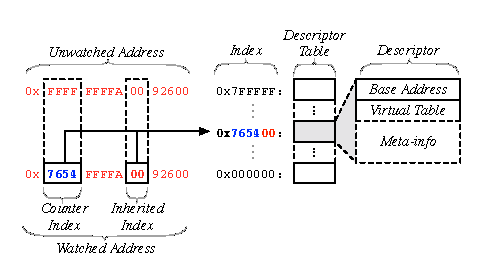
\epsfig{file=watchpoints.eps, width=3.0in, height=1.4in}
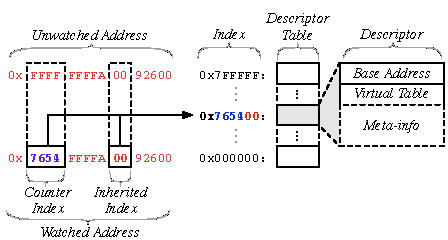
\includegraphics[width=6.0in]{watchpoints.pdf}
\end{center}
\vspace{-15pt}
\caption[Design of behavioral watchpoints.]{\label{fig:watchpoint_descriptor_table}A watched address (bottom left) and its corresponding unwatched address (top left) are compared. The watched address takes the form of non-canonical address that are not addressable in kernel space. The watchpoint framework uses a \emph{counter index} and an \emph{inherited index} to store the descriptor information in a global descriptor table. The process of resolving the watchpoint descriptor is shown.}
%for the watched address is shown.}
\end{figure}


Our design of behavioral watchpoints is geared to the 64 bit x86 (x86-64) architecture. In kernel space on the x86-64 architecture, the addressable memory includes the canonical form of addresses with their 16 high-order bits set to 1. Tagging these higher order bits with the descriptor information converts them to a non-canonical address that triggers a hardware exception when dereferenced. The watchpoint framework takes advantage of the exception to implement behavioral watchpoints.

%The design of behavioral watchpoint is shown in \Figref{watchpoint_descriptor_table}. It uses 15 high-order bits (called the \emph{counter index}) and an additional 8 bits (bits 20-27, called the \emph{inherited index}) of a watched address to identify the index into a global \emph{watchpoint descriptor table} which stores the pointer to the watchpoint's descriptor. %This extends the number of possible watchpoints to 8M. 
%The key advantage of our watchpoint scheme is the ability to directly map watched addresses to unwatched addresses using a simple bitmask. One drawback of the scheme is that an offset of a watched address can cause the low-order bits to overflow into the inherited index. We overcome this issue by assigning multiple descriptors for the watched objects holding the same meta-information and by putting them in adjacent indices. 

%is to manage multiple descriptors for a watched object.

%The watched addresses are non-canonical addresses that trigger a hardware exception when dereferenced. 
%We take advantage of the x86-64 architecture for implementing watched addresses. In kernel space on x86-64, canonical addresses have their 16 high-order bits set to 1. Watched addresses do not take this form; they are non-cannonical addresses that trigger a hardware exception when dereferenced. 
Our watchpoint framework uses two approaches to perform memory operations on watched objects. First, when watchpoints are expected to be triggered frequently, it dynamically adds instrumentation at every memory load and store to avoid hardware exceptions. Watched addresses are detected before they are dereferenced and resolved to their unwatched counterparts (by masking the 16 high-order bits to 1). The approach is called code-centric instrumentation because the decision about the code translation and instrumentation is taken based on the execution path. 
Second, when watchpoints are unlikely to be triggered, the alternative approach is to dereference a watched address and implement behavioral watchpoints in the trap handler. This enables on-demand binary translation and allows adding instrumentation only when a watchpoint is triggered. We call this approach data-centric instrumentation because code translation and instrumentation is based on watchpoint accesses.


%We call it the data-centric instrumentation which enables the feature of adding selective instrumentation. The approach takes decision about code translation and instrumentation based on the access of watchpoints. 


%, which lowers the overhead of binary translation. % when watchpoints are fewer in number and unlikely to be triggered. 

The design of behavioral watchpoints provides the following benefits:
\begin{enumerate}[i)]
\item \emph{\textbf{Multiple watchpoints can watch the same range of memory:}} 
Two copies of an address (e.g., two pointers to the same object) can be watched separately, so long as the high-order bits index different entries in the watchpoint descriptor table. %they manage different descriptors. 
This is useful for distinguishing between logically different objects that occupy the same memory region. For example, this enables efficient detection of use-after-free bugs without preventing deallocated memory from being immediately reallocated for another use. This efficiency comes from our ability to have one watchpoint for the freed object and another watchpoint for the newly allocated memory occupying the same space.

\item \emph{\textbf{Watchpoint descriptors are context specific:}} 
Our design separates the allocation and management of descriptors from the watchpoint framework. It is the responsibility of each client to manage its descriptors. When a watchpoint gets added to an object, the client determines the \emph{vtable}, \emph{type} and \emph{meta-information} that needs to be stored in the descriptor, as shown in \Figref{watchpoint_descriptor_table}. The vtable determines the function that is invoked when watched memory is accessed. Each vtable provides eight functions: four read and four write functions. Each function is specific to a memory operand size (1, 2, 4, or 8 bytes). A watchpoint descriptor is initialised with either a generic or a type-specific vtable, which is specific to the \emph{type} of the watched address. The meta-information allows the descriptors to be arbitrarily customized or extended based on the needs of the client.

\item \emph{\textbf{Watchpoints are viral:}}
Behavioral watchpoints can be used virally. If an address $A$ is watched, then every address derived from $A$ (e.g., through copying or offsetting) is also watched. This is useful for memory and taint analysis tools. For instance, a watchpoint that is added early in the lifetime of an address (e.g., immediately before the address of newly allocated memory is returned from an allocator) can persist and propagate until no more derived addresses exist.
\end{enumerate}

%Behavioral watchpoints earn their name from vtable because they allow watchpoints to behave differently when watched memory is accessed.


%A watchpoint's descriptor is indirectly located by interpreting these high-order bits as an index into a global \emph{watchpoint descriptor table} which stores the pointer to watchpoint's descriptor(\Figref{watchpoint_descriptor_table}). 
%Because these bits do not change, many addresses end up indirectly referring to the same watchpoint descriptor.

%\subsection{Design Implications}
%Our approach has the following design implications.

%Any unwatched address can be converted into an watched address. The extra level of indirection added by watching an address allows us to efficiently locate context-specific information about the memory being watched.

%A watchpoint is added to a program by changing the high-order order bits of an address used by the program. 
%Watchpoints work on ranges instead of individual units of memory because a watchpoint is added to a program by changing 

%\paragraph{A watched address must be distinguishable from an unwatched address.} 

%Behavioral watchpoint framework provides API \emph{add\_watchpoints()} which is used to add watchpoints to an arbitrory object. It takes the obeject address and size to creates the descriptor for the object. The descriptor can be based on the type or size of the object. The descriptor can be changed dynamically if required. The descriptor is then stored into descriptor table at the next free index generated by counter and partial index. If some object doesn't need descriptor they are only assigned the watched address with corrosponding index in the descriptor table assigned NULL. 

%Behavioral watchpoint provides support where two copies of an address (e.g., two pointers to the same object) can be separately watched, so long as they manage different descriptors, the high-order bits index different entries in the watchpoint descriptor table. 
%This is useful for distinguishing between logically different objects that occupy the same memory. For example, this feature enables efficient detection of use-after-free bugs without preventing deallocated memory from being immediately reallocated for another use. This efficiency comes from our ability to have one watchpoint for the freed memory, and another watchpoint for newly allocated memory occupying the same space.


%\paragraph{Multiple watchpoints can watch the same range of memory.} Two copies of an address (e.g., two pointers to the same object) can be separately watched, so long as they manage different descriptors. %the high-order bits index different entries in the watchpoint descriptor table. 
%This is useful for distinguishing between logicallywatchpoint framework  different objects that occupy the same memory. For example, this feature enables efficient detection of use-after-free bugs without preventing deallocated memory from being immediately reallocated for another use. This efficiency comes from our ability to have one watchpoint for the freed memory, and another watchpoint for newly allocated memory occupying the same space.

%\paragraph{Millions of watchpoints are supported.} Our design as described uses 15 high-order bits (called the \emph{counter index}) and additional 8 bits (bits 20-27, called the \emph{inherited index}) of a watched address for identifying a watchpoint's descriptor.  This extends the number of possible watchpoints to 8M.  %and is left unchanged when converting an unwatched address into a watched address.
%The key advantage of our watchpoint scheme is the ability to directly map watched addresses to unwatched addresses using a simple bitmask. The main drawback of the scheme is that an offset of a watched address can cause the low-order bits to overflow into the inherited index. One solution to overcome this problem is to manage multiple descriptors for a watched object. 

%Our design allows the same range of memory to be watched differently. For example, two pointers to the same object can be watched separately, so long as they manage different descriptors. This feature is useful for distinguishing logically different objects that occupy the same memory. For example, this feature enables efficient detection of use-after-free bugs without preventing deallocated memory from being immediately reallocated for use. Having one watchpoint for the freed memory, and another watchpoint for newly allocated memory occupying the same space, is critical for this application. %Watchpoint gets added with a call to \texttt{ADD\_WATCHPOINT} which takes the reference of object and corrosponding meta-information as parameter. \texttt{REMOVE\_WATCHPOINT} is used to remove watchpoint from a watched object. 

%For example, this feature enables efficient detection of use-after-free bugs without preventing deallocated memory from being immediately reallocated for another use. This efficiency comes from our ability to have one watchpoint for the freed memory, and another watchpoint for newly allocated memory occupying the same space.

%We are exploring several solutions to this problem.

% This counter index extends the number of possible watchpoints to 8M and is left unchanged when converting an unwatched address into a watched address. The key advantage of our watchpoint scheme is the ability to directly map watched addresses to unwatched addresses using a simple bitmask. The main drawback of the scheme is that an offset of a watched address can cause the low-order bits to overflow into the counter index. We are exploring several solutions to this problem.

% and 8 bits (bits 20-27, called the \emph{inherited index}) for identifying a watchpoint's descriptor

%of a watched address for identifying a watchpoint's descriptor. 15 bits only allows 32K watchpoints. To increase the number of watchpoints, we use an additional 8 bits (bits 20-27, called the \emph{inherited index}) in the address to index into the watchpoint descriptor table (\Figref{watchpoint_descriptor_table}). This counter index extends the number of possible watchpoints to 8M and is left unchanged when converting an unwatched address into a watched address. The key advantage of our watchpoint scheme is the ability to directly map watched addresses to unwatched addresses using a simple bitmask. The main drawback of the scheme is that an offset of a watched address can cause the low-order bits to overflow into the counter index. We are exploring several solutions to this problem.

%\paragraph{Millions of watchpoints are supported.} Our design as described uses 15 of the 16 high-order bits (called the \emph{counter index}) of a watched address for identifying a watchpoint's descriptor. 15 bits only allows 32K watchpoints. To increase the number of watchpoints, we use an additional 8 bits (bits 20-27, called the \emph{inherited index}) in the address to index into the watchpoint descriptor table (\Figref{watchpoint_descriptor_table}). This counter index extends the number of possible watchpoints to 8M and is left unchanged when converting an unwatched address into a watched address. The key advantage of our watchpoint scheme is the ability to directly map watched addresses to unwatched addresses using a simple bitmask. The main drawback of the scheme is that an offset of a watched address can cause the low-order bits to overflow into the counter index. We are exploring several solutions to this problem.

%This approach has some drawbacks when an offset of a watched address causes the low-order bits to overflow into the counter index; however, we have several solutions to this problem. 

%\paragraph{Watchpoint descriptors are context-specific.} Our design separates the allocation and management of descriptors from the watchpoint framework. It is the responsibility of each client to manage its descriptors. %, which % and declare the corrosponding descriptor type for the framework. provides complete flexibility in handling it. 
%When a watchpoint gets added to an object, the client determines the \emph{type}, \emph{meta-information} and \emph{vtable} which needs to be stored in the descriptor. These descriptors can be arbitrarily customized or extended based on the needs of the client. %One powerful application of this extension is discussed in section~\ref{sec:access_policies}.




%This aspect of watchpoints is possible because our design separates the allocation/management of descriptors and the addresses that they watch. When a watchpoint is added to an address, the \emph{type} or \emph{size} of the address determines what meta-information is included in the descriptor, as well as what function to invoke when memory watched by the watchpoint is accessed. These descriptors can be arbitrary customized or extended based on the needs of program analysis tools. Two powerful applications of this extension are discussed in \Secref{type_overflow} and \Secref{access_policies}.


%Arbitrary extension of descriptors supports our goal of overcoming the incongruency between the needs of debugging an analysis tools (contextual information about watched memory), and how existing software implements watchpoints (watched memory is opaque).

%\subsection{Extensions}
%Our design includes the following extensions to watchpoints, which expand on the behavioral aspect of our watchpoint implementation.
%principally enable the \emph{behavioral} aspect of our software-based watchpoint .
%Our goal of using watchpoints to watch the memory of objects required the following 

%\paragraph{Watchpoints are type-specific.} When a watchpoint is added to an address, the \emph{type} of the address determines what meta-information is included in the descriptor, as well as what functions to invoke when memory watched by the watchpoint is accessed. Two powerful applications of this extension are discussed in \Secref{type_overflow} and \Secref{access_policies}.

%\paragraph{Triggered watchpoint functions are polymorphic.} The function invoked when watched memory is accessed is decided using a descriptor-specific \emph{vtable}. Each vtable provides eight functions: four read and four write functions. Each function is specific to a memory operand size (1, 2, 4, or 8 bytes). A watchpoint descriptor is initialised with either a generic or a type-specific vtable, which is specific to the \emph{type} of the watched address. %Behavioral watchpoints earn their name from vtable because they allow watchpoints to behave differently when watched memory is accessed.

%When invoked, a vtable function operates on the watched address and its descriptor. Behavioral watchpoints earn their name from their ability to behave differently based on the meta-information stored in the descriptor and the (type-specific) vtable function invoked.

%\paragraph{Watchpoints remember their originating address.} The address to which a watchpoint is first added is called its \emph{base address}, and is stored in the watchpoint descriptor. We designed watchpoints to remember their base address because it helps to ``anchor" contextual information. When a watchpoint is added, \emph{something} is known about the watched address. Later in a program's execution, an offset of the watched address might be dereferenced. Little can be said about the dereferenced address in relation to the watchpoint's originating address without knowing the originating address.

%Without the former context of why or where the watchpoint was originally added, there is little that can be said about the relation between the triggered address and 
%the watched memory except that it might be arbitrarily far away from the address to which the watchpoint was originally added.
%That is, something is known about an address when the decision to add a watchpoint to that address is made. 
%If the original address is not remembered, then it is difficult to relate a triggered watchpoint
%We designed watchpoints this way so that at any point during the lifetime of a watchpoint, 
%Watchpoints were designed this way so that contextual information is always ``anchored" to something that was once known. 

%This is consistent with our goal of using watchpoints to watch the memory of an object because we expect the base address to be the address in memory of a watched object.

%Watchpoint desc

%Because watchpoints are added to addresses, and 

%This means that 


%We can change an address into a \emph{watched address} by ensuring that a watched address is non-canonical: it cannot legally be used (on x86) without triggering a hardware exception.


%changing part of an address, not by 
%The watched range is \emph{anchored} on the address on which the watchpoint is initially added (called the base address). 

%Behavioral watchpoints are implemented by changing an address to-be-watched into a non-canonical address\footnote{In kernel space on x86, a canonical virtual address has its 16 high-order bits set to 1. Current x86 processors require that the 8 high-order bits of an address match the $9^{th}$ highest order bit.}. The translation from unwatched to watched alters the unused high-order bits of an address. 

%There are several implications of this design decision:
%\begin{enumerate}
%	\item 
%\end{enumerate}



%Behavioral watchpoints were designed with the following goals in mind:
%\begin{enumerate}
%	\item 
%\end{enumerate}

%\subsection{Design Challenges}
%The design of behavioral watchpoint put following restrictions in the way it can be used:
%\begin{enumerate*}
%\item[i)] A watchpoint must be added at the object source. Adding watchpoints at arbitrary location must be avoided since there is a possibility of another unwatched copy of the same object existing in the program data. This will introduce incosistency and object will be partially watched.
%\item[ii)] Behavioral watchpoints can't be used in applications playing with high-order bits. Such operation will introduce incosistency in descriptor information attached with watched addresses. Applications doing similar things like depending on sign-extension of the 64-bit addresses or handling of 32-bit addresses is also not supported. Identifying and ignoring such cases is a problem and we are exploring solutions to this.
%\item[iii)] Behavioral watchpoints are implemented for Linux kernel and one should be careful when using page-table lookup for watched addresses. Operations such as \texttt{\_\_pfn\_to\_page} and \texttt{\_\_page\_to\_pfn} can lead to wrong \texttt{page} structure or loss of descriptor information.
%One should also be careful when using kernel functions for page-table lookup on watched addresses.
%We found some cases where fast method of mapping virtual addresses to physical addresses for page table lookup was depending on sign extension of 64-bit addresses which is not the case when it is changed to watched addresses. 

 %can't be used in applications playing with high-order bits. Such operation will introduce incosistency in descriptor information attached with watched addresses. Applications doing similar things like depending on sign-extension of the 64-bit addresses or handling of 32-bit addresses is also not supported. Identifying and ignoring such cases is a problem and we are exploring solutions to this.
%\end{enumerate*} 

%put some restrictions on the range of applications which it can handle. Behavioral watchpoint tags the higer-order bits with the descriptor information and it can't handle the application which is also doing similar things. Such operation will corrupt the embedded descriptor information and once lost we don't have a way to recover it. Identifying applications doing such operation is challenging. Applications which are only handling with 32-bit address is also not supported. We designed behavioral watchpoints for the Linux kernel but all the functionalities in the kernel is not very suitable for the approach. We found some cases where fast method of mapping virtual addresses to physical addresses for page table lookup was depending on sign extension of 64-bit addresses which is not the case when it is changed to watched addresses. 

%has the following design implications. 

%are designed for Linux kernel and generated by providing an extra-level of indirection and storing the descriptor information in higher order bits of the address. This puts restrictions on the range of applications which behavioral watchpoints can handle. The applications storing tagging information with the high-order bits of the address works against the design of behavioral watchpoints. Identifying such operations in an application is an open problem for us. Our solution of embedding descriptor information in object address is not very friendly with some of the kernel functions.   


%However identifying such operations in an application is an  


%However all the applications  


%The operation is not very friendly with some of the kernel functions. Linux kernel uses fast method of mapping virtual addresses to physical address. The mapping functions performs bit-operations in the  


%and virtual address into struct pages for lookup in the page table. 


 %to the physical address. These operations 


%There is a requirement for Linux to have a fast method of mapping virtual addresses to physical addresses and for mapping struct pages to their physical address. Linux achieves this by knowing where, in both virtual and physical memory, the global mem_map array is because the global array has pointers to all struct pages representing physical memory in the system. All architectures achieve this with very similar mechanisms, but, for illustration purposes, we will only examine the x86 carefully. This section will first discuss how physical addresses are mapped to kernel virtual addresses and then what this means to the mem_map array.   

%\subsection{Architecture}

%The implementation of behavioral watchpoints distinguishes between watched addresses and their descriptors.

%A \emph{watched address} is a pointer with an index into the \emph{watchpoint descriptor table} embedded in its bits (\Figref{watchpoint_descriptor_table}). The $23$-bit index into the descriptor table is formed by concatenating bits $[20,27]$ (called the \emph{counter index}) with bits $[48,62]$ (called the \emph{partial index}). A watched address and its unwatched counterpart share the same counter index; however, the partial index of a watched address varies\footnote{This feature of watchpoints allows for a one-to-one mapping between a watched and unwatched address, and a one-to-many mapping between a watchpoint and all addresses watched by that watchpoint. The one-to-one mapping is formed by masking the high-order bits containing the partial index.}. Partial indexes are recorded in the \emph{partial index counter table}. When a watchpoint is allocated, the current value stored in the counter table for that specific counter index is incremented and returned as the watchpoint's partial index. This allocation strategy allows for at most $2^{15}$ watchpoints per counter index or megabyte of memory\footnote{x86 has byte-addressable memory. The counter index begins at bit $20$, giving each watchpoint $1$ MB = $2^{20}$ B degrees of freedom. However, if an over/underflow across the 1 MB-aligned boundary occurs then the counter index will be corrupted. We can correct one bit of corruption by requiring that the counter index and the partial index have the same sign. An alternative solution is uses a different indexing scheme. We have successfully experimented with a different indexing scheme that solves the aforementioned overflow errors, but sacrifices the one-to-one relationship between a watched and unwatched address.}.

%A \emph{watchpoint descriptor} is a data structure containing a base address, a pointer to a virtual table (vtable) of memory operations, and programmer-defined meta-information.



\section{Implementation}
Behavioral watchpoints are implemented using Granary, a dynamic binary translation (DBT) framework \cite{GranaryAtOSDI} described in Chapter~\ref{sec:Granary}. %Granary instruments arbitrary, binary Linux kernel modules efficiently and without imposing overhead when the core kernel is running. Our implementation uses Granary because it allows us to analyze and debug kernel modules, which are a frequent source of bugs and vulnerabilities in operating systems \cite{BGI,LXFI}.
%
%
%is to use Granary to analyse and debug kernel modules, which are a frequent source of bugs and vulnerabilities in operating systems \cite{BGI,LXFI}.
%
%Granary is unique among DBT systems because it provides three important features: i) mixed-mode execution, ii) policy-driven instrumentation, and iii) reifying instrumentation. The \emph{mixed-mode execution} allows the watchpoint framework to switch the execution between instrumented and native mode implicitly or with the wrapper interface. Granary achieves this by substituting the execution of a function with a \emph{wrapped} version of itself. A wrapped function has the same type specification as its unwrapped counterpart and can freely modify its arguments and return value. Granary can wrap some module functions in this way, even if the module source code is unavailable.
%
%The \emph{policy-driven instrumentation} enables the watchpoint framework track and specialise the instrumentation with the execution context. The knowledge of the execution context helps the framework make decision on adding new watchpoints or collecting the added watchpoints. It also allows the framework to efficiently manage the \emph{context-specific} information in the watchpoint's descriptor.
%
%The \emph{reifying instrumentation} provides the high-level static analysis information to the watchpoint framework. This provides the framework ability to specialise the instruction-level instrumentation with higher-level abstractions. Writing such powerful instrumentation code using low-level DBT abstractions of Granary is hard and it motivated the design of behavioral watchpoint framework.
%
%
%it analyzes and uses static type information of the program. For example, Granary can substitute the execution of a function with a \emph{wrapped} version of itself. 
%A wrapped function has the same type specification as its unwrapped counterpart and can freely modify its arguments and return value. Granary can wrap some module functions in this way, even if the module source code is unavailable. 
%
%While Granary provides a framework for instrumenting kernel modules, we found it was hard to write powerful instrumentation code using low-level DBT abstractions, which motivated the design of behavioral watchpoints. %Next, we describe examples of watchpoint-based debugging applications developed for kernel modules.
%
%\vspace{0.5em}
%Behavioral watchpoints take the form of non-canonical addresses. To implement the behavioral watchpoint, the framework writes the watchpoint instrumentation code for every memory accesses. Granary inserts the watchpoint instrumentation code before every memory load and store instructions before putting them into code-cache. 
We implement behavioral watchpoints by adding watchpoint instrumentation before every memory read (load) and write (store) instruction in the code cache. The watchpoint instrumentation actively looks for non-canonical addresses being used as a source or destination address and triggers watchpoint handling code if it encounters them. The watchpoint framework provides an interface for the client to write the watchpoint handling code efficiently. Our approach of implementing the watchpoint framework has three advantages: %There is two advantages our current approach of watchpoint implementation:

%In order to implement the behavioral watchpoint framework, there is a need to write watchpoint instrumentation for every memory read and write operations. Granary inserts this watchpoint instrumentation code before every memory load and store instructions before putting them into code-cache. These watchpoint instrumentation code actively looks for the non-canonical addresses being used as one of the source or destination target address and triggers watchpoint handling code when it encounters the watched addresses. The current approach of implementing behavioral watchpoints has two advantages: %re is two advantages our current approach of watchpoint implementation:
 %checking code before every memory load and store instructions before putting them in code-cache. The watchpoint checking code actively looks for the non-canonical addresses being used as source or destination addresses and triggers the watchpoint handling code when it encounters the watched addresses. There is two advantages our current approach of watchpoint implementation:
\begin{enumerate}[i)]
	\item The framework makes it easy to add watchpoints with the object. It provides an indirection to the memory address of the unwatched object and tags it with the counter index. It separates the allocation and management of descriptors and provides the client an interface to manage its own descriptors. The framework only manages the global descriptor table and assigns the descriptors to the corresponding indices. %The framework manages the global descriptor table and assign the descriptors in corresponding indices. %  It also sets the descriptor for the watched objects and  %It needs to set the counter index tag with the associated address of the watched objects and sets the 
	 %makes it easy to add watchpoints with the object of interest. We only need to set the counter index tag with the associate address of a watched object and update the corresponding information about the watched objects in the descriptor and global descriptor table. The watchpoint framework takes care of inserting instrumentation before every load and store before putting them in code-cache. Any further execution of the module happens from the code-cache.
	\item The direct mapping of watchpoints with the descriptors make the descriptor information available when the watched objects are accessed. This is helpful in specialising the instrumentation based on the descriptor's information.
	\item The runtime overhead of watchpoint implementation comes from the watchpoint instrumentation. Our implementation of watchpoint instrumentation has a fixed cost and the overhead does not increase drastically with the increase in the number of watchpoints.
\end{enumerate}



\begin{figure*}
\begin{multicols}{2}
\lstset{language=[x64]Assembler, numbers=left, label=Original}
\begin{lstlisting}[basicstyle=\footnotesize\ttfamily, caption=Original instructions]
mov    %rbx,0x340(%r13)
mov    $0x400,%esi
mov    %rax,0x80(%rbx)
\end{lstlisting}
%\label{list:Original}
\lstset{language=[x64]Assembler, numbers=left}
\begin{lstlisting}[basicstyle=\footnotesize\ttfamily, caption=Translated instructions]
lea    0x340(%r13),%rsi
bt     $0x30,%rsi
jb     addr_not_watched_2
bt     $0x2f,%rsi
jae    addr_not_watched_2
callq  granary_bounds_check_8_rsi
bswap  %rsi
mov    $0xffff,%si
bswap  %rsi
LABEL: addr_not_watched_2
mov    %rbx,(%rsi)
mov    $0x400,%esi
push   %rcx
lea    0x80(%rbx),%rcx
bt     $0x30,%rcx
jb     addr_not_watched_3
bt     $0x2f,%rcx
jae    addr_not_watched_3
callq  granary_bounds_check_8_rcx
bswap  %rcx
mov    $0xffff,%cx
bswap  %rcx
LABEL: addr_not_watched_3
mov    %rax,(%rcx)
pop    %rcx
\end{lstlisting}
\label{fig:translated}
\columnbreak
\lstset{language=[x64]Assembler, numbers=left,  label=Overflow}
\begin{lstlisting}[basicstyle=\footnotesize\ttfamily, caption=Overflow detector]
granary_bounds_check_8_rsi :
pushfq 
push   %rax
push   %rdi
push   %r8
mov    %rsi,%rdi
mov    %rsi,%r8
mov    %rsi,%rax
shl    $0x24,%r8
shr    $0x38,%r8
shr    $0x31,%rdi
shl    $0x8,%rdi
or     %r8,%rdi
lea    0x192c98(%rip),%r8   		# 0xffffffffa03cf280 <client::wp::DESCRIPTORS>
lea    (%r8,%rdi,8),%rdi
mov    (%rdi),%rdi
cmp    (%rdi),%eax
jl     overflow_detected
mov    %rax,%r8
add    $0x7,%r8
cmp    %r8d,0x4(%rdi)
jle    overflow_detected
jmp    no_overflow_detected
LABEL : overflow_detected
callq  buffer_overflow_handler
LABEL : no_overflow_detected
pop    %r8
pop    %rdi
pop    %rax
popfq  
retq  
\end{lstlisting}
\end{multicols}
\caption[The baseline watchpoint instrumentation and the instrumentation for buffer overflow detector.]{The native and instrumented version of the instructions performing the basic memory operations. The translated instruction (Listing~\ref{Original}) shows the watchpoint instrumentation required for detecting watchpoints and performs the memory operation at the watched addresses. The buffer overflow detector (Listing~\ref{Overflow}) gets triggered only if the addresses are watched. The overflow detector makes a call to \texttt{buffer\_overflow\_handler} if the overflow is detected. %and sample code for checking read critical section. It checks the violation of Rule0 and verfify that RCU protected data is accessed inside read critical section.
}
\label{fig:mem-write}
\end{figure*}

%The watchpoint framework enables two approach of implementing behavioral watchpoints: the code-centric and the data-centric approach. The code-centric approach provides comprehensive instrumentation by following all execution path, translating and adding the basic blocks in the code cache lazily. The data centric approach selectively perform the instrumentation on demand. Both the approaches takes advantage of the features of granary and provides powerful infrastructure for developing analysis tools. Each approach also has its advantages and disadvantages which is discussed below.

%Behavioral watchpoints framework is implemented to provides support for three instrumentation approaches: the code-centric, the data-centric and mixed instrumentation. Each of them has its own advantages and disadvantages. The program analysis tools developed using watchpoint framework uses these approaches to optimize their performance.  


\subsection{Code-Centric Instrumentation}
The Code-centric instrumentation dynamically adds watchpoint instrumentation at every memory reference before putting each basic block in code-cache. Code-centric watchpoint instrumentation detects the dereference of watched addresses and resolves them to their unwatched counterparts before performing the memory operation, thus avoiding any hardware traps that would be generated if a watched address is accessed directly. Code-centric instrumentation has low overhead when compared with trap based instrumentation when watchpoints are expected to be triggered frequently.
%The code-centric instrumentation provides comprehensiveness by following the execution path and translating the basic blocks. It avoids the hardware traps by executing the instrumented version of code from the code-cache. The watchpoint instrumentation detects the dereference of watched addresses and resolve them into their unwatched counterparts before performing the memory operations. 
%The approach benefits from the low cost of instrumentations when the watchpoints are expected to be triggered frequently. The comprehensive instrumentation also benefits from the warm code-cache effect avoiding the cost of translation and instrumentation for future execution.

We implemented behavioral watchpoints using Granary, which comprehensively instruments all module code. Granary detaches itself at the kernel interface thus providing support for code-centric instrumentation only for module code. A module analysis tool developed using the watchpoint framework may need to track the behavior of objects that are shared between the kernel and a module using watchpoints. 
For these shared objects, we use code-centric instrumentation for the module code, and trap-based or data centric instrumentation (with the transitive policy, as described in
the next section) for the kernel code.


%These watched objects often gets leaked to the kernel and dereference of such addresses results in hardware traps. The Granary with its code-centric instrumentations can not avoid these traps.

%In our implementation, the watchpoint framework also provides the code-centric instrumentation only for the module code. It avoids the hardware traps in the kernel code using on-demand data centric instrumentation. Our policy for kernel code uses transitive instrumentation which minimizes the overhead of hardware traps.

%re is high probability of dereferencing watchpoint addresses.




%takes control of the module code and dynamically add
%Behavioral watchpoints take the form of non-canonical addresses that trigger a hardware exception when dereferenced. This design of behavioral watchpoint enables the opportunity of data-centric instrumentation. This enable adding instrumentation selectively by attaching and detaching instrumentation framework on demand, introducing overhead only when they are needed. This approach benefits from the lower overhead of binary translation when several watchpoints are likely to be triggered, and the lower overhead of infrequent traps when watchpoints are unlikely to be triggered. In our implementation of behavioral watchpoints for the kernel modules we used binary translation for the module code and trap-based instrumentation for the kernel code. The instrumentation strategy is based on the assumption that the watchpoint addresses leaked to the kernel are less likely to be get accessed and for such watchpoints, instrumenting entire kernel code will be costly.


\subsection{Data-Centric Instrumentation}\label{sec:data-centric}
Data-centric instrumentation is triggered by hardware traps when a watched address is dereferenced. At this point, Granary is attached so that code can be instrumented. We used three policies for detaching instrumentation: i) basic-block instrumentation, ii) function-only instrumentation, and iii) transitive instrumentation. % and iv) thread instrumentation.

The basic block instrumentation policy detaches instrumentation at the end of the current basic block. This policy translates the minimum amount of code but causes the highest number of traps.

The function-only policy retains the same instrumentation policy across the body of a function and does not allow the transfer of policy across control-transfer instructions. The framework stops instrumenting and detaches itself at the end of function body (i.e, with the \texttt{ret} instruction). Any \texttt{call} to other functions detaches the framework temporarily and then the framework is attached once that function returns. The policy instruments a moderate amount of code with a corresponding decrease in the number of hardware traps, compared to the basic block policy.% the increase in the number of hardware traps. 

The transitive policy allows the framework to follow the code-centric instrumentation transferring its instrumentation policy across the \texttt{call} or \texttt{jmp} instructions; the framework detaches itself when the function returns. The transitive policy instruments code aggressively based on the assumption that once the watched address is dereferenced in an execution path, there is high probability of encountering the watchpoints again in the same function or the functions called by this function. Our evaluation result supports this assumption.

The ability to add selective instrumentation by attaching and detaching the watchpoint framework on demand introduces overhead only when instrumentation is needed. The data-centric approach benefits from the lower overhead of infrequent traps when watched addresses are less likely to be dereferenced, e.g., when watchpoints are added selectively for a few objects.


% . The data-centric instrumentation suffers from the high overhead of hardware traps and particularly useful for watching the selective objects. 

%dereference, e.g., when watchpoints are added selectively for a few objects.

 %and the framework detaches itself when there is a policy change at the indirect control-transfer. The policy translates and instruments maximum code and put them into code-cache. This avoids the future hardware traps due to the access of watched objects. We designed this policy based on the assumption that once the watched address is dereferenced in an execution path, there is high probability of encountering the watchpoints again in the same function or the functions called by it. Our evaluation result supports this assumption.


%The transitive policy  


%The design of behavioral watchpoint enables the opportunity of data-centric instrumentation. The data-centric approach allows the framework add watchpoint instrumentation selectively on demand. The data-centric instrumentation gets triggered by the hardware traps, which happens due to the dereference of watched addresses. The hardware traps allows Granary to attach the instrumentation framework on a memory dereference of watched objects and detaches itself on the next control-transfer instructions.

%The data-centric approach provides three different instrumentation policies: i) transitive instrumentation, ii) function-only instrumentation, and iii) basic block instrumentation. 

%The transitive instrumentation allows the framework to transfer its instrumentation policy across the \texttt{call} or \texttt{jmp} instructions and the framework detaches itself when there is a policy change at the indirect control-transfer. The policy translates and instruments maximum code and put them into code-cache. This avoids the future hardware traps due to the access of watched objects. We designed this policy based on the assumption that once the watched address is dereferenced in an execution path, there is high probability of encountering the watchpoints again in the same function or the functions called by it. Our evaluation result supports this assumption.

%The function-only instrumentation retains the same instrumentation policy across the body of a function and does not allow the transfer of policy across control-transfer instructions. The framework stops instrumenting and detaches itself at the end of function body (i.e, with the \texttt{ret} instruction). Any \texttt{call} to other functions detaches the framework temporarily which gets attached once that function returns. The policy instruments moderate amount of code with the increase in the number of hardware traps. 

%The basic-block instrumentation policy is conservative in its approach of dynamically adding the translated basic block in code-cache. The policy is true in its nature of on-demand instrumentation and translates a basic block at a time when required. It also does not allow the transfer of instrumentation policy across the control transfer and the instrumentation framework detaches itself at the end of basic block. The policy translates minimum amount of code and handles maximum number of hardware traps. 
 %and instrumentation framework detaches itself on the first encounter of the control transfer instructions.

%The ability to add selective instrumentation by attaching and detaching the watchpoint framework on demand introduces overhead only when instrumentation is needed. The data-centric approach benefits from the lower overhead of infrequent traps when watched addresses are less likely to be dereferenced. The data-centric instrumentation suffers from the high overhead of hardware traps and particularly useful for watching the selective objects. 

%During our evaluation we noticed that the selective instrumentation also suffers from the high overhead due to cold code-cache effect. However, this could be avoided by following the transitive instrumentation policy. The data-centric approach provides an opportunity for optimising the code-centric instrumentation where the hardware traps can be used to switch policy between null and watcpoint instrumentation. We have not yet implemented this optimisation for our code-centric instrumentation approach.  

%does not allow the transfer of instrumentation policies across a control transfer and instrumentation framework detaches itself on the first encounter of the control transfer instructions. The policy instruments minimum of the module or the kernel code to avoid the watchpoint instrumentation cost. However it suffers from the high cost of traps as the number of hardware-exceptions encountered in this  policy increases significantly. 

%policy does not allow the transfer of instrumentation policies on control-transfer instruction but it retains the same policy for instrumenting the function body. The policy only instruments the body of the functions to avoid any further traps by the watched objects.


%high likely of encountering the watchpoints again in the same function or in any function called by it.


%This policy instruments the maximum code once the framework is attached to avoid the high cost of hardware exception. The policy is designed based on the assumption that once the watched address is encountered there is high likely of encountering the watchpoints again in the same function or in any function called by it.


 %by attaching and detaching watchpoint framework on demand introduces overhead only when they are needed. The approach benefits from the lower overhead of infrequent traps when watched addresses are less likely to be dereferenced.




%and it gets detached on next control-transfer instructions or the end of function-body based on the instrumentation policy.

%----

%Behavioral watchpoints are implemented using an extra-level of indirection to the memory addresses. The watched addresses take the form of non-canonical address that trigger a hardware exception when dereferenced. This design of behavioral watchpoint enables the opportunity of data-centric instrumentation. The hardware traps allows Granary to attach the instrumentation framework on a memory dereference of watched objects and it gets detached on next control-transfer instructions or the end of function-body based on the instrumentation policy.

%The ability to add instrumentation selectively by attaching and detaching watchpoint framework on demand introduces overhead only when they are needed. The approach benefits from the lower overhead of infrequent traps when watched addresses are less likely to be dereferenced.

%The data-centric instrumentation provides three policies for instrumenting the module and the kernel code : i) transitive policy, ii) function-body policy, and iii) basic block policy. 

%Transitive policy allows the framework to transfer the policy across \texttt{call} or \texttt{jmp} and the framework detaches only on the indirect calls. This policy instruments the maximum code once the framework is attached to avoid the high cost of hardware exception. The policy is designed based on the assumption that once the watched address is encountered there is high likely of encountering the watchpoints again in the same function or in any function called by it.

%Function-only policy does not allow the transfer of instrumentation policies on control-transfer instruction but it retains the same policy for instrumenting the function body. The policy only instruments the body of the functions to avoid any further traps by the watched objects.

%Basic-block policy does not allow the transfer of instrumentation policies across a control transfer and instrumentation framework detaches itself on the first encounter of the control transfer instructions. The policy instruments minimum of the module or the kernel code to avoid the watchpoint instrumentation cost. However it suffers from the high cost of traps as the number of hardware-exceptions encountered in this  policy increases significantly. 

 %In our implementation of behavioral watchpoints for the kernel modules we used binary translation for the module code and trap-based instrumentation for the kernel code. The instrumentation strategy is based on the assumption that the watchpoint addresses leaked to the kernel are less likely to be get accessed and for such watchpoints, instrumenting entire kernel code will be costly.or

%\subsection{Mixed Instrumentation}
%Mixed instrumentation enables the opportunity for both code-centric and data-centric instrumentation. The approach benefits from the low overhead of dynamic instrumentation when then there is high likely hood of encountering watchpoints and low overhead of data-centric instrumentation when the watchpoints are less likely to be dereferenced. 


\subsection {Instrumentation Optimizations}
The implementation of behavioral watchpoints essentially requires monitoring of all memory read (load) and write (store) operations. A basic monitoring framework using dynamic binary instrumentation inserts new instructions before every memory references looking for the watchpoint addresses. The framework also inserts watchpoint instrumentation before every memory operation. A naive implementation of watchpoint instrumentation performs the following operations:
\begin{enumerate}[i)]
	\item Save and restore the registers, including flags registers, that are used or affected by watchpoint instrumentation. We use the stack to spill these registers. 
% (stack is used to spill these registers). Also spill the flags if watchpoint instrumentation touches any of the flags.
	\item Calculate the referenced address and check if this is one of the non-canonical addresses. This is done by inspecting high-order 16 bits of the addresses. Inject a callback function, if the address is in the non-canonical form. This requires the masking of both user and kernel space addresses. The 47th and 48th bit of the address is reserved and used for this purpose.
	\item Emulate the actual instruction with corrected address to perform the normal load/store operation and continue execution after restoring registers and flags. The instruction emulation is done by replacing the original instruction or by creating a new instruction and providing an indirection.
	\item Continue the normal execution after restoring the registers and flags, if the address is not one of the watched addresses.
\end{enumerate}

The naive implementation of watchpoint instrumentation suffers from high runtime overhead. Granary allows implementing several optimizations for reducing runtime overhead. The watchpoint instrumentation uses the following optimizations:
\begin{enumerate}[i)]
	\item \emph{\textbf{Dead Registers Analysis}:} The instrumentation system needs scratch registers for creating and injecting new instructions. These registers can be obtained by spilling them to the stack or to memory locations. The frequent spilling of these registers on stack or memory location increases the cost of instrumentation significantly~\cite{Probst02registerliveness, Muth98registerliveness}. Granary provides support for managing live registers. It goes over the basic block, performs the register liveness analysis and collects all the registers that can be safely used without spilling them on the stack. The register manager traverses all the instructions in a basic block moving upward and collecting the source and destination registers making all the non-source and non-base-displacement registers (whole destination registers) as dead.

	\item \emph{\textbf{Flag Liveness Analysis}:} In an instrumentation system, the newly injected instructions should not affect the state of the processor. The watchpoint instrumentation ensures this by saving and restoring the status registers before and after the injected instructions. This is costly and so the framework reduces this cost by performing eflag liveness analysis~\cite{Dynst2011}. The watchpoint instrumentation saves and restores the flags register only if it is alive.

	\item \emph{\textbf{Eliminate Stack Operations}:} In the x86 architecture, any operation on the stack or an operation involving the stack pointer is also a memory operation. Watchpoint instrumentation is not required for these memory operations unless it is specified by the client. The watchpoint framework identifies all such instructions and prevents them from getting instrumented. 	Applications such as the stack-based overflow detector require instrumenting any operation involving stack pointers and they need to specifically add such instrumentation. 
	 %Watchpoint instrumentation system performs the register liveness analysis on each basic block to identify registers that can be safely used without requiring it to spill on the stack. For register liveness analysis, instrumentation system starts instrumenting from the end of the basic block moving upward and collecting all the source and destination registers making all the non source and non base-displacement registers (whole destination registers) as dead. Watchpoint instrumentation also performs the eflag Liveness analysis~\cite{Dynst2011} and save and restore flags only if it is alive.
\end{enumerate}

Figure~\ref{fig:mem-write} shows the native and instrumented versions of the instructions performing memory operations. The DBT system provides several other optimizations such as \emph{Group Checks}, which consolidate the two consecutive memory reference checks into a single check if there are no intervening instructions that affect address generation, and \emph{Merge Checks} which exploit the locality of memory references and merge the instrumentation for instructions accessing different members of the same object in the same basic block. We have not implemented all these optimizations in the watchpoint framework because our purpose is not to be exhaustive but rather to demonstrate that watchpoint instrumentation can perform online monitoring of memory references with reasonable overhead.



\section{Limitations}
The design of behavioral watchpoints introduces non addressable memory in the system. The use of non-canonical addresses puts the following restrictions on the way watchpoints can be used. Some of these limitations are application specific and depend on how the program analysis tool uses them.
\begin{enumerate}[i)]
	\item The behavioral watchpoint framework suggests adding watchpoints early in the life of the objects. Adding watchpoints at an arbitrary location should be avoided as it can introduce inconsistency in the program. A program running with both watched and unwatched versions of the same object will provide only partial information about the object. However some program analysis tools such as RCU debugger takes advantage of this limitation and generates two versions of the same objects, each of them getting watched differently.
	%A watchpoint must be added at the object source. Adding watchpoints at arbitrary location must be avoided since there is a possibility of another unwatched copy of the same object existing in the program data. This will introduce incosistency and object will be partially watched.
	\item Behavioural watchpoints uses high-order bits to store the descriptor information. The descriptor provides the \emph{meta-informations} about the object being watched. This puts restriction on the use of behavioral watchpoints in analysing applications which play with the high-order bits of its addresses. Such application will destroy the descriptor information stored with the watchpoints. Applications doing the similar operations such as sign extension of the 64-bit addresses or handling of only 32-bit addresses also loses the descriptor information. The watchpoint framework has no mechanism to recover the lost descriptor information from the watchpoints. Identifying and ignoring such applications or the operations in an application is an important challenge for the watchpoint framework.  

%Identifying and ignoring such cases is a problem and we are exploring solutions to this.
	\item Behavioural watchpoints are implemented for the Linux kernel. The Linux kernel uses bitwise operations for the fast page-table lookup. These bitwise operations converts the virtual page addresses into the page frame number and assumes that the 16 high-order bits of the addresses are all one. Linux kernel also maintains different address space regions and perform different functions for the page table-lookup. The design of behavioral watchpoints are not friendly with these operations.

	%and one should be careful when using page-table lookup for watched addresses. Operations such as pfn to page and page to pfn can lead to wrong page structure or loss of descriptor information.
\end{enumerate}


\section{Evaluation}\label{sec:approach_eval}
In this section, we evaluate the performance overhead of behavioral watchpoints. The watchpoint framework implements behavioral watchpoints by injecting instrumentation for every memory read (load) and write (store) operations, introducing runtime overhead in the system. We evaluated the cost of watchpoint instrumentation, including the cost of handling hardware traps for data-driven instrumentation, using synthetic microbenchmarks. 


%The behavioral watchpoints also introduces the concept of data-driven instrumentation that triggers the selective instrumentation on hardware traps. We used microbenchmark to evaluate the cost of handling hardware traps.  

We also measured the overhead of using behavioral watchpoints on the throughput of common file I/O operations using the \emph{iozone}~\cite{citeulike:919086} file system benchmark and the performance of real-world workloads using several file system utilities and the Filebench benchmarks. 
%We also evaluated the overhead of the watchpoint framework on file system utilities and measure the performance of real-world workload using filebench.
We ran all our experiments on a desktop equipped with an Intel\textregistered\ Core\texttrademark\ 2 Duo 2.93 GHz CPU with 4GB physical memory. In our experimental setup, we used the \texttt{ext3} file system module that was mounted on a 1GB RAMDisk (mounting loads the \texttt{ext3} and \texttt{jbd} journaling kernel modules). The watchpoint framework wraps the kernel memory allocators to add watchpoints for all newly allocated objects.

%\textbf{TODO}: explain why we are using filesystem module and iozone for the evaluation


%We also evaluated the overhead of using behavioral watchpoint framework on common file operations.


%Microbenchmark is used to evaluate the cost of watchpoint instrumentation which is required for identifying the watchpoints and performing the memory operations at the watched addresses. We used \emph{Iozone}~\cite{citeulike:919086} filesystem benchmark for measuring the overhead of behavioral watchpoints on common filesystem operations. In our experimental setup, the \texttt{ext3} filesystem was mounted on a 1GB RAMDisk (mounting loads the \texttt{ext3} and \texttt{jbd} journaling kernel modules). We also evaluated the overhead of using behavioral watchpoint framework on common file operations.
%We implemented behavioral watchpoint framework which provides support to instrument module code. Hence, behavioral watchpoints provides support for two approaches: data-driven and mixed instrumentation. 



\begin{table*}
\begin{center}
%\begin{centering}
\begin{tabular}{|l|c c c|}
  \hline
  Optimizations & Native & Watch Null & Watch All \\
  \hline
  Code-driven (with BB optimizations)  & 1x & 2.7x & 3.8x \\
  \hline
  Code-driven (without BB optimizations) & 1x & 5.0x &	6.2x \\
  \hline
  Data-driven approach  & 1x & 1x & 283x \\
  \hline
\end{tabular}
\caption[Performance impact of watchpoint instrumentation on microbenchmark.]{\label{table:microbenchmark_optimizations}The performance overhead of watchpoint instrumentation on a synthetic microbenchmark (\Figref{microbenchmark}). The code-driven approach evaluates the cost of using watchpoint instrumentation and the benefit of basic block optimizations. The overhead of the data-driven approach is dominated by the cost of handling hardware traps.}
\end{center}
\end{table*}


\begin{figure}
\begin{lstlisting}[language=C,basicstyle=\footnotesize\ttfamily]

typedef unsigned long long cycles_t;
cycles_t currentcycles() {
    unsigned cycles_low, cycles_high;
     __asm__ __volatile__ (
			"cpuid\n\t"
			"rdtsc\n\t"
			"mov %%edx, %0\n\t"
			"mov %%eax, %1\n\t": "=r" (cycles_high), 
			"=r"(cycles_low):: "%rax", "%rbx", "%rcx", "%rdx");

    return ((unsigned long long)cycles_low) 
		| (((unsigned long long)cycles_high) << 32);
}
enum {
	NUM_OUTER = 10,
	NUM_INNER = 100000
};

/* Initialize the LKM */
volatile unsigned long x[2] = {100, 200};
int init_module() {
    int i,j;
    unsigned long addr;
    unsigned long flags;
    volatile struct foo_test *ptr = 
		(struct foo_test*)kmalloc(sizeof(struct foo_test), GFP_KERNEL);

    cycles_t before[NUM_OUTER], after[NUM_OUTER];

    for(j=0; j < NUM_OUTER ; j++)
    {
	preempt_disable();
	raw_local_irq_save(flags);
    	before[j] = currentcycles();
    	for(i = 0; i < NUM_INNER; ++i) {
		__asm__  volatile("mov %rax, %rax;");
		(ptr)->l1 += x[i % 2];
		__asm__  volatile("mov %rax, %rax;");
    	}
    	after[j] = currentcycles();
	raw_local_irq_restore(flags);
	preempt_enable();
    }
  
    return 0;
}
\end{lstlisting}
\vspace{-10pt}
\caption[The synthetic microbenchmark used to evaluate the watchpoint framework.]{\label{fig:microbenchmark}Synthetic microbenmark used to evaluate the watchpoint instrumentation. It performs basic memory operation inside a tight-loop.}
\end{figure}

\subsection{Microbenchmark}
Our microbenchmark consists of a tight-loop of memory operations that exhibits the worst-case overhead of using watchpoint instrumentation. \Figref{microbenchmark} shows the synthetic microbenchmark we used to evaluate the overhead of watchpoint instrumentation and hardware traps. We also evaluated the benefits of our optimization schemes such as register-liveness analysis and flag-liveness analysis used for watchpoint instrumentation. We call this basic block optimizations. 

Table~\ref{table:microbenchmark_optimizations} shows the maximum cost of using watchpoint instrumentation and handling a hardware trap. \emph{Watch None} represents the overhead of baseline watchpoint instrumentation when no watchpoints have been added, and \emph{Watch All} shows the overhead when all module allocated objects are being watched. The added overhead of \emph{Watch All} comes due to the indirection required for masking watched addresses and emulating the original instructions. 


Table~\ref{table:microbenchmark_optimizations} also shows the high overhead of handling hardware traps. In the data-centric approach, the hardware trap triggers the instrumentation of the module code. The high overhead of a hardware trap shows that the approach is useful for selective instrumentation when watchpoints are less likely to be triggered. 

%The \emph{watchpoint\_null} does not add any overhead because the hardware traps never gets triggered and instrumented code never gets executed.






\begin{figure}[t]
\begin{center}
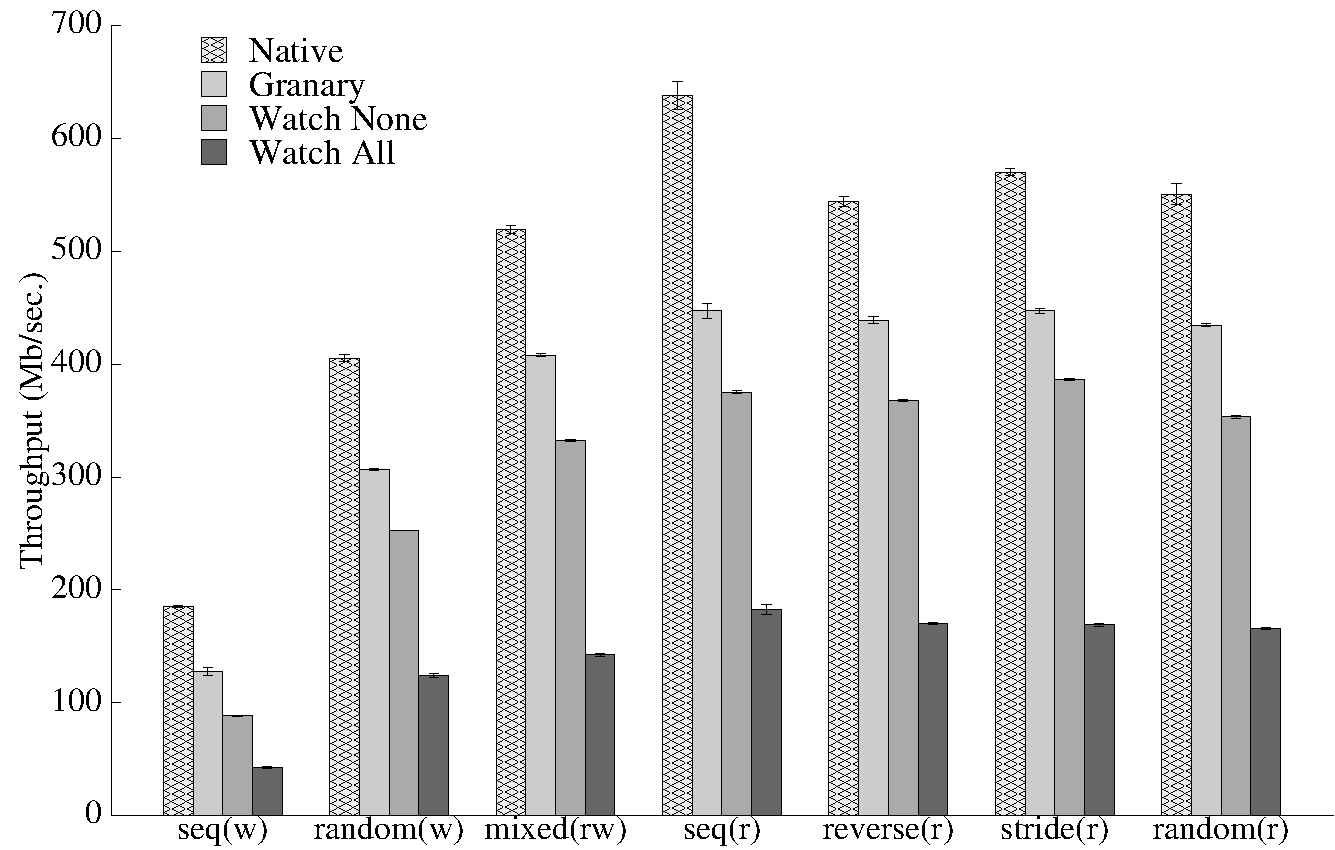
\includegraphics[width=4.5in]{thesis_code_driven.pdf}
\end{center}
\caption[Performance impact of code centric instrumentation.]{\label{fig:watchpoint_performance_code_driven}Throughput in MB/sec of common file system operations for code-centric instrumentation. Direct IO is enabled to bypass the effect of the OS buffer cache on read requests. It compares the overhead of the watchpoint framework with the performance overhead of Granary and with native system.}
\end{figure}

\subsection{Iozone filesystem benchmark}
We used the \emph{iozone}~\cite{citeulike:919086} file system benchmark to measure the overhead of behavioral watchpoints on the throughput of common file system operations. In our experimental setup, we used the \texttt{ext3} file system module that was mounted on a RAMDisk of size 1GB. We enabled direct IO to avoid the effect of buffer cache on file system. The \emph{iozone}, in throughput mode, created two processes (reader, writer) that perform the file I/O operations on a file of size 480Mb with a record size of 4Kb. The watchpoint framework wraps the two most commonly used memory allocators in \texttt{ext3} and \texttt{jbd}: \texttt{\_\_kmalloc} and \texttt{kmem\_cache\_alloc}, to add watchpoints on the allocated objects. We evaluated both the code-centric \& data-centric approaches using \emph{iozone} and compared their performance.


%----

%We evaluated both code-centric and data-centric approach using \emph{iozone} and compared their performance in terms of the number of active watchpoints. 
%In data-centric instrumentation approach the behavioral watchpoint does not uses wrappers for attaching and detaching Granary at the interface. The framework attaches on traps raised by dereferencing of watched addresses and it detaches at the end of basic block or when the function returns. In this case we wrap the allocators by hot-patching kernel text and add watchpoints only when the allocation happens by the module code. 

\begin{table*}
\begin{center}
\vspace{1em}
\begin{tabular}{|l|r|r|}
  \hline
  \multicolumn{3}{|c|}{Watchpoint statistics for the code-centric instrumentations}  \\ \hline
  \hline
  & Watch None & Watch All \\
  \hline
  Number of basic blocks & 2249 & 5495\\
  \hline
  Number of basic blocks with watched memory operations & 0 & 1208\\
  \hline
  Number of executed basic blocks & 238782485 &  825836778 \\
  \hline
  Number of dynamic memory operations & 568643857 & 1693113417 \\
  \hline
  Number of watched memory operations & 0 &199495293 \\
  \hline
  Number of kernel hardware traps & 0 & 12630779 \\
  \hline
\end{tabular}
\caption[Watchpoint statistics for code centric instrumentation. The watchpoints are added on all module allocated objects.]{\label{table:code-centric-watchpoint_stats} The statistics of the watchpoint framework for code-driven instrumentation when module allocated objects are watched. It also shows the effect of watched objects leaked to the kernel. The increase in the number of hardware traps causes an increase in the number of basic blocks and the number of executed basic blocks.}
\end{center}
\end{table*}

\paragraph{Code-centric instrumentation:}
The code-centric approach comprehensively instruments the module code and dynamically adds watchpoint instrumentation at every memory reference. This baseline watchpoint instrumentation causes overhead even when there are no added watchpoints. In the code-centric approach the module always runs under the control of Granary and executes code from the code-cache. It uses the kernel and module function wrappers for fast attaching and detaching at the interface. %This causes an extra overhead on any interactions between the kernel and the modules.

In the code-centric instrumentation, we first evaluated the overhead of watchpoint instrumentation and the cost of using Granary as the underlying DBT system. This is important to understand the baseline cost of using the watchpoint framework. 

\Figref{watchpoint_performance_code_driven} represents the overhead of code-centric instrumentation on the throughput of file I/O operations. The overhead of the watchpoint framework increases to {\texttildelow}70\% when all objects allocated by the module are watched. This is because many of these watched objects are shared and leak to the kernel. When these objects are dereferenced in the kernel, they cause hardware traps because Granary detaches itself at the kernel interface and the watchpoint instrumentation is no longer added to the memory references. These hardware traps are costly and reattach the watchpoint framework which then instruments the kernel code transitively.


\begin{table*}
\begin{center}
%\caption{Performance of macrobenchmark}
\begin{tabular}{ |l||r|r|r| }
\hline
\multicolumn{4}{ |c| }{Access pattern of module allocated objects} \\ \hline
\hline
Memory Allocator & Size & Module Accesses Count  & Kernel Accesses Count\\ \hline
\multirow{5}{*}{$\_\_kmalloc$} & 8 & 1233865 & 0 \\ \cline{2-4}
 & 50 & 720 & 288\\ \cline{2-4}
 & 51 & 648 & 240\\ \cline{2-4}
 & 59 & 792 & 528\\ \cline{2-4}
 & 4096 & 23452 & 0 \\ \hline
 \hline
 \multirow{7}{*}{$kmem\_cache\_alloc$} & 16 & 31533 & 0 \\ \cline{2-4}
 & 24 & 25019188 & 0\\ \cline{2-4}
 & 32 & 2348 & 0\\ \cline{2-4}
 & 64 & 2469028 & 3099\\ \cline{2-4}
 & 112 & 21404553 & 0 \\ \cline{2-4}
 & 192 & 19902520 & 4916028 \\ \cline{2-4}
 & 768 & 57760206 & 37373718 \\ \cline{2-4}
 & 1024 & 34865132 & 7940485 \\ \cline{2-4}
 & 8196 & 299 & 821648 \\ \hline
 \hline
 \multirow{1}{*}{$\_get\_free\_page$} & 4096 & 820273 & 2973 \\ \hline
\end{tabular}
\caption[Memory access pattern of module allocated objects.]{\label{table:access_pattern_shared_objects}The memory accesses patten of the module allocated objects. It represents the number of times an object is getting accessed by the module and the kernel code. The objects are classified based on its size and the memory allocator used for allocation. %The post analysis  shows that file system \texttt{inode} objects with memory size 768 are most accessed object by the kernel. A watchpoint on \texttt{inode} object will generate maximum number of hardware traps.
}
\end{center}
\end{table*}

\begin{table*}
\begin{center}
\vspace{1em}
\begin{tabular}{|l|r|r|}
  \hline
  \multicolumn{3}{|c|}{Watchpoint statistics for the code-centric instrumentations}  \\ \hline
  \hline
  & Watch none \texttt{inode} & Watch All \\
  \hline
  Number of basic blocks & 2874 & 5495\\
  \hline
  Number of basic blocks with watched memory operations & 732 & 1208\\
  \hline
  Number of executed basic blocks & 266083908 &  825836778 \\
  \hline
  Number of dynamic memory operations & 594195510 & 1693113417 \\
  \hline
  Number of watched memory operations & 92600064 &199495293 \\
  \hline
  Number of kernel hardware traps & 5285701 & 12630779 \\
  \hline
\end{tabular}
\caption[Watchpoint statistics for code centric instrumentation. The watchpoints are added on all the module allocated objects except file \texttt{inode}s.]{\label{table:code-centric-node-inode-watchpoint_stats} The watchpoint statistics of the framework for code-driven instrumentation when all objects allocated by the modules (except \texttt{inode}s) are watched.}
\end{center}
\end{table*}

Table~\ref{table:code-centric-watchpoint_stats} represents the number of hardware traps encountered and number of executed basic blocks for the code centric instrumentation. The additional increase in the number of basic blocks ({\texttildelow}2.5{\footnotesize$\times$}) and the number of executed basic blocks ({\texttildelow}3.5{\footnotesize$\times$}) comes due to the kernel code instrumentation on hardware traps. It also shows that the one out of every sixteen watched memory operations causes hardware traps.

For understanding the source of these hardware traps, we developed a tool using the watchpoint framework which tracks the accesses of module allocated objects. We typed these objects based on their size and the memory allocator used for its allocation. Table~\ref{table:access_pattern_shared_objects} shows the access pattern of the module allocated objects. The post processing analysis shows that file system \texttt{inode} objects with its size ``768'' gets accessed by the kernel maximum number of times and adding watchpoint on \texttt{inode} objects cause maximum number of hardware traps.

We verified this by removing watchpoints from all \texttt{inode} objects and running \emph{iozone} in throughput mode. \Figref{watchpoint_performance_code_driven_none_inode} shows that the overhead for \emph{Watch All} decreases by {\texttildelow}50\% and is close to the overhead of baseline instrumentation i.e, \emph{Watch None}. The small differences in the overhead of \emph{Watch All} and \emph{Watch None} are because there were still some shared objects which was getting watched and causing hardware traps. Table~\ref{table:code-centric-node-inode-watchpoint_stats} shows the details about such objects.


\begin{figure}[t]
\begin{center}
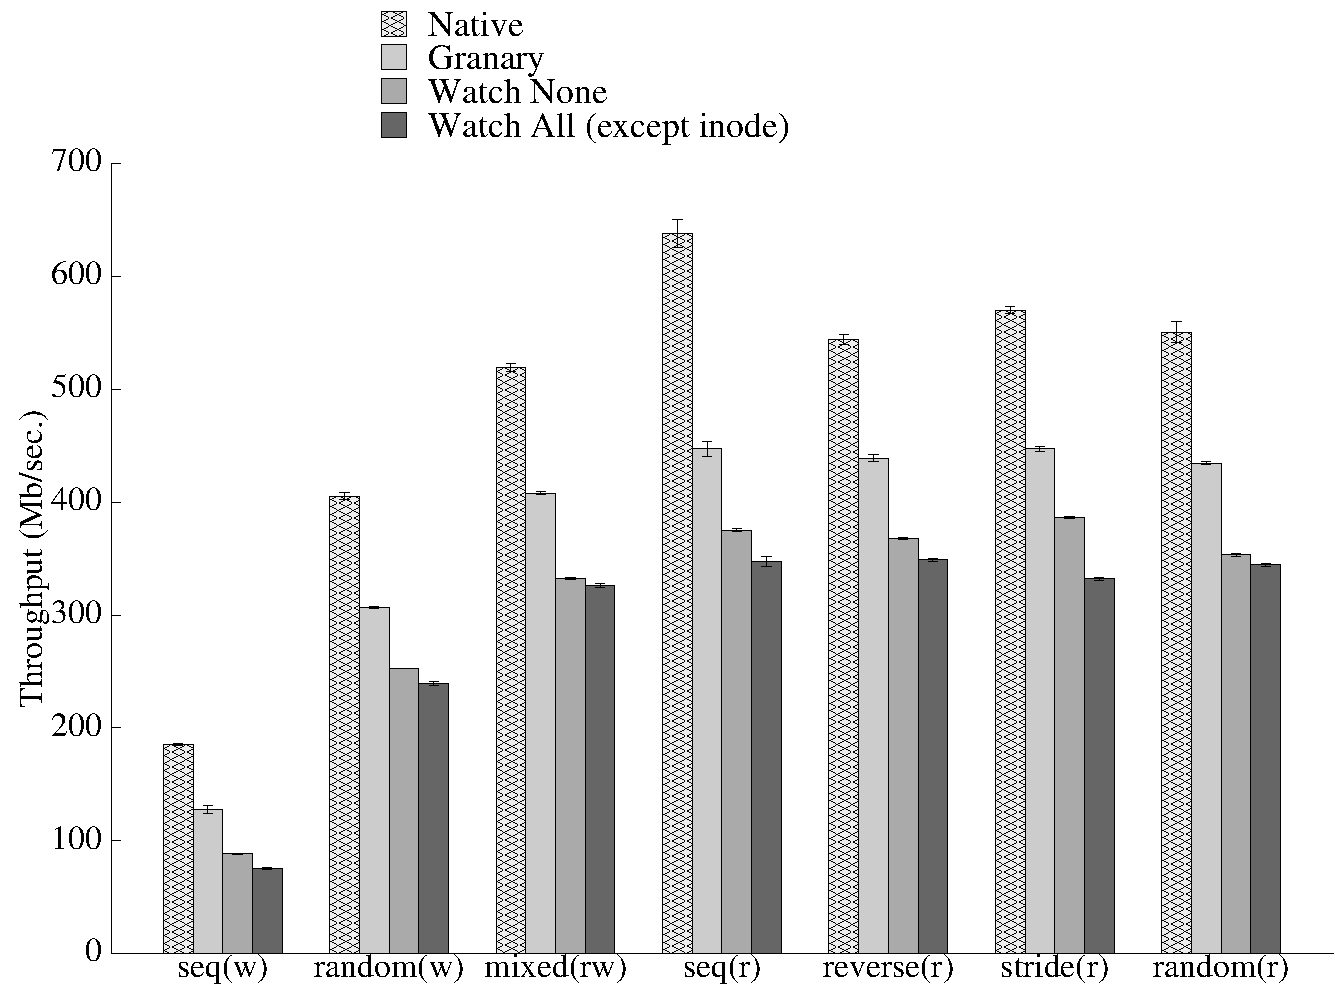
\includegraphics[width=4.5in]{thesis_code_none_inode.pdf}
\end{center}
\caption[Performance impact of code centric instrumentation. The watchpoints are added on all module allocated objects except file \texttt{inode}s.]{\label{fig:watchpoint_performance_code_driven_none_inode}Throughput in MB/sec of common file system operations for code-centric instrumentation when \texttt{inode} objects are not getting watched. The overhead of \emph{Watch All} decrease because of the less number of hardware traps and executed basic blocks.}
\end{figure}


The evaluation of code-centric instrumentation shows that the hardware traps on the kernel code are the major source of overhead in implementing behavioral watchpoints. These hardware traps can be removed by providing full kernel support to the code-centric instrumentation. Granary, being the underlying DBT-system, currently does not provide support for whole kernel instrumentation. 

%To understand the source of these hardware traps, we developed a tool using the watchpoint framework 


%We also studied the source of these hardware traps 


%The evaluation shows that a major contribution in the overhead of code-centric instrumentation comes due to Granary and its wrapping mechanism.

 %\Figref{watchpoint_performance_code_driven} shows the drop in throughput of filesystem operations when using the watchpoints instrumentation. As mentioned earlier \emph{watchpoint\_null} represents the overhead of baseline watchpoints instrumentation with no added watchpoints, and \emph{everything\_watched} shows the overhead where module-allocated objects are watched. We used code-centric instrumentation approach for the evaluation.

%In the previous section, we discussed that due to the limitations of Granary to instrument only the module code, our implementation of code-centric instrumentation is limited. We use code-centric instrumentation for executing the module code and data-centric instrumentation for the kernel code if the watchpoint leaks to the kernel. We also use three different policy for the code-centric instrumentation: transitive instrumentation policy, function-only instrumentation policy and basic-block instrumentation policy. The detail about these policies are discussed in section. Before evaluating the complete data-centric approach, we evaluated the compared the effect of three policies on code-centric instrumentation.



%\Figref{watchpoint_performance_code_driven} shows the overhead on the throughput of different filesystem operations. We also collected the watchpoint statistics for the the three policies. Table~\ref{table:data-centric-table} shows the number of hardware-exception encountered and the ration of executed basic block containing watched and unwatched addresses.

\begin{figure*}[t]
\begin{center}
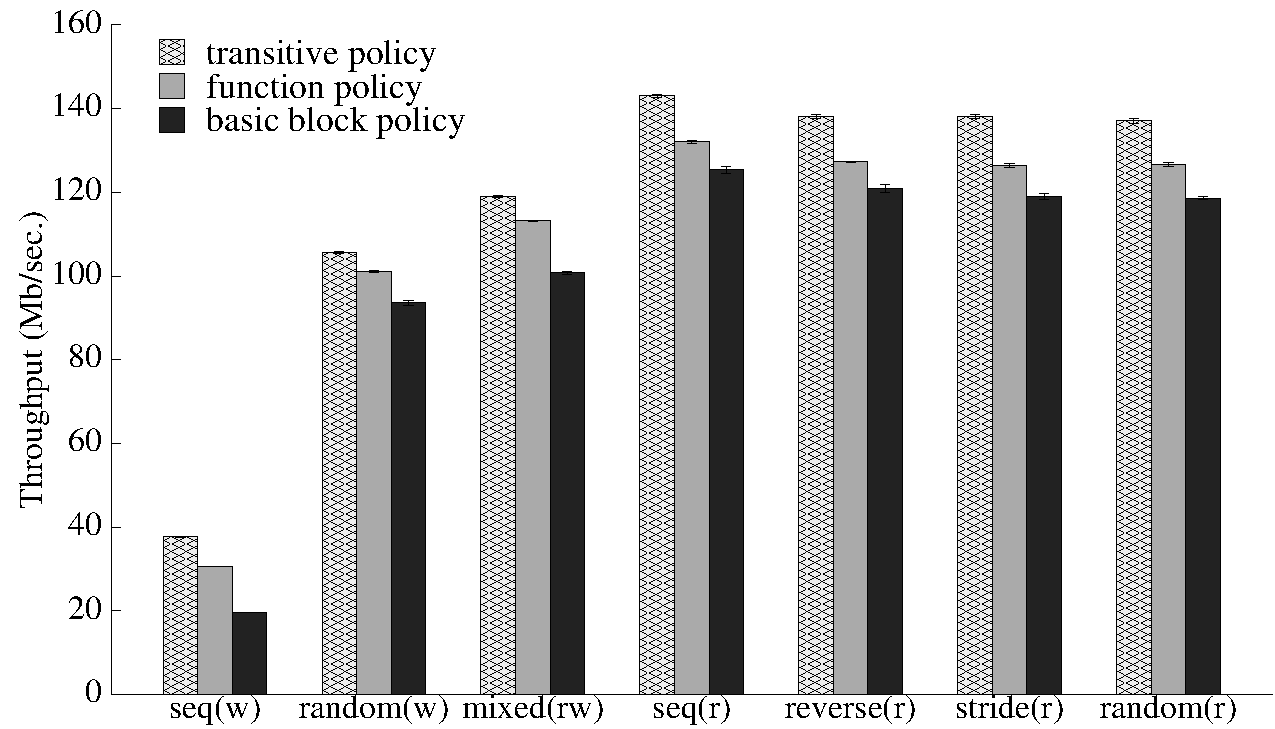
\includegraphics[width=4.5in]{thesis_data_driven.pdf}
\end{center}
\caption[Performance impact of data centric instrumentation.]{\label{fig:watchpoint_performance_data_driven}Throughput in MB/sec of common file system operations for data-centric instrumentation. It shows the overhead of three data-centric policies: transitive policy, function only, and basic block only policy.}
%for the watched address is shown.}
\end{figure*}


\paragraph{Data-centric instrumentation:}
We implemented data-centric instrumentation with three detach policies: i) transitive policy, ii) function-only policy and iii) basic block policy. Section~\ref{sec:data-centric} discusses each of the three policies in detail. %The data-centric instrumentation adds watchpoints on newly allocated objects through hot-patching and wrapping the kernel memory allocators. 


\begin{table*}
\begin{center}
\vspace{1em}
\begin{tabular}{|l|r|r|r|}
  \hline
  \multicolumn{4}{|c|}{Watchpoint statistics for data-centric instrumentation (with different detach policies)}  \\ \hline
  \hline
  & transitive & function & block \\
  \hline
  Number of basic blocks & 5755 & 3335 & 1144 \\
  \hline
  Number of basic blocks with watched memory operations & 1479 & 1218 & 1141\\
  \hline
  Number of executed basic blocks &  833167407  & 108965164 & 37378155\\
  \hline
  Number of dynamic memory operations & 1702295819 & 565666812 & 251985370\\
  \hline
  Number of watched memory operators & 336149753 & 234340514 & 206334774\\
  \hline
  Number of kernel hardware traps & 13403663 & 42259345 & 97518601\\
  \hline
  Number of module hardware traps & 112172 & 23496407 & 42902684\\
  \hline
\end{tabular}
\caption[Watchpoint statistics for data centric instrumentation.]{\label{table:data-centric-table} The statistics of the watchpoint framework for data-centric instrumentation when all the objects allocated by the modules are watched. It compares the three detach policies used by the data-centric approach.}
\end{center}
\end{table*}

We evaluated the overhead of data-centric instrumentation with \emph{iozone}, using the same experimental setup as with the code-centric instrumentations. We disabled the kernel and the module wrappers since they allow Granary to take complete control over the module code and prohibit the module code from running native. In data-centric instrumentation, the module code gets executed natively when there are no added watchpoints. 

Before comparing the code-centric and data-centric approaches, we first evaluated the three detach policies of data-centric instrumentation. \Figref{watchpoint_performance_data_driven} shows the overhead of each policy on the throughput of file I/O operations. The transitive policy instruments code aggressively and performs better than the function only and basic block detach policies. Table~\ref{table:data-centric-table} shows the number of executed basic blocks and the number of hardware traps encountered when each of the three detach policies are used. The transitive policy encounters the minimum number of hardware traps and executes the largest number of basic blocks. %The transitive policy also has large number of basic block with watched memory operations and this is because it adds more number of watchpoints on the newly allocated objects.

% executes the module code natively when no watchpoints get added and does not cause any runtime overhead in the system. It also uses three policies to reduce the cost of handling hardware traps. We first evaluated the three policies of data-centric instrumentation and compared their performance overhead along with the number of basic block executed and the hardware traps encountered by each of them. \Figref{watchpoint_performance_data_driven} shows the overhead of each policies on the throughput of file I/O operations for \texttt{ext3} module. The transitive policy has slight advantage over the function only and basic block policy because of the decrease in the number of hardware traps it needs to handle. There is also an increase in the number of basic block executed and this adds to the overhead of the transitive policy. Table~\ref{table:data-centric-table} shows how the number of executed basic blocks and the number of hardware traps encountered varies across the three policies. It also shows that the number of hardware traps encountered in module code is always less than the hardware traps at the kernel code. It represents that a majority of watched objects are shared and leaks to the kernel. These hardware traps also causes a significant overhead in the code-centric instrumentation and our approach of code-centric is more biased towards the data-centric.


\begin{figure}[t]
\begin{center}
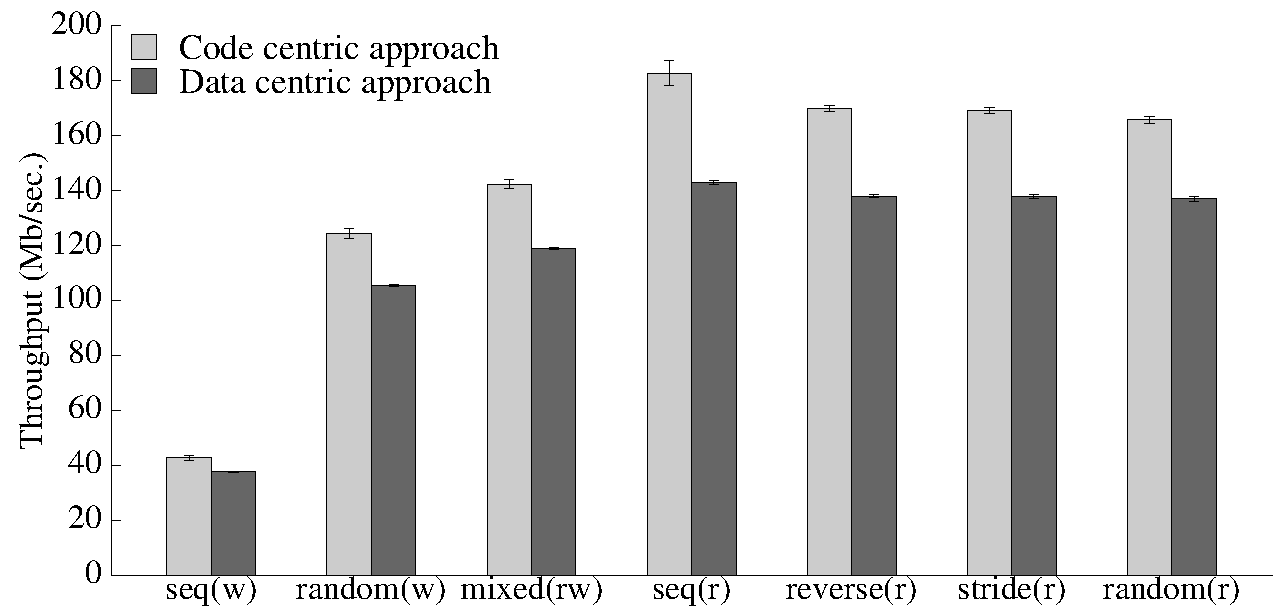
\includegraphics[width=6.0in]{thesis_data_code.pdf}
\end{center}
\caption[Performance impact of Data centric Vs Code centric instrumentation.]{\label{fig:watchpoint_performance}Throughput in MB/sec of common file system operations for the code-centric and data-centric approaches. The watchpoints are added on all objects allocated by the module.}
%for the watched address is shown.}
\end{figure}

%of the two reasons: i) the data-centric instrumentation handles more hardware traps which is costly, and ii) the number of watchpoints added in transitive detach policy is more than the code-centric instrumentations.

%In spite of increase in the number of hardware traps in the data-centric approach, it is performing better than the code-centric approach. This is because of the increase in the number of executed basic blocks. Also the code-centric approach suffers significantly due to the large number of hardware traps in the kernel code. The evaluation of three policies of data-centric approach also shows that the increase in the overhead due to hardware traps is getting compensated with the less number of basic block being executed. Table~\ref{table:data-centric-table} shows that the number of hardware traps encountered in transitive policy is 5x less than the basic block policy but it is executing 10x more basic block and thus not getting much advantages in terms of performance. The code centric approach is also using the kernel and the module wrappers which has an additional cost.

\begin{figure}[!h]
\begin{center}
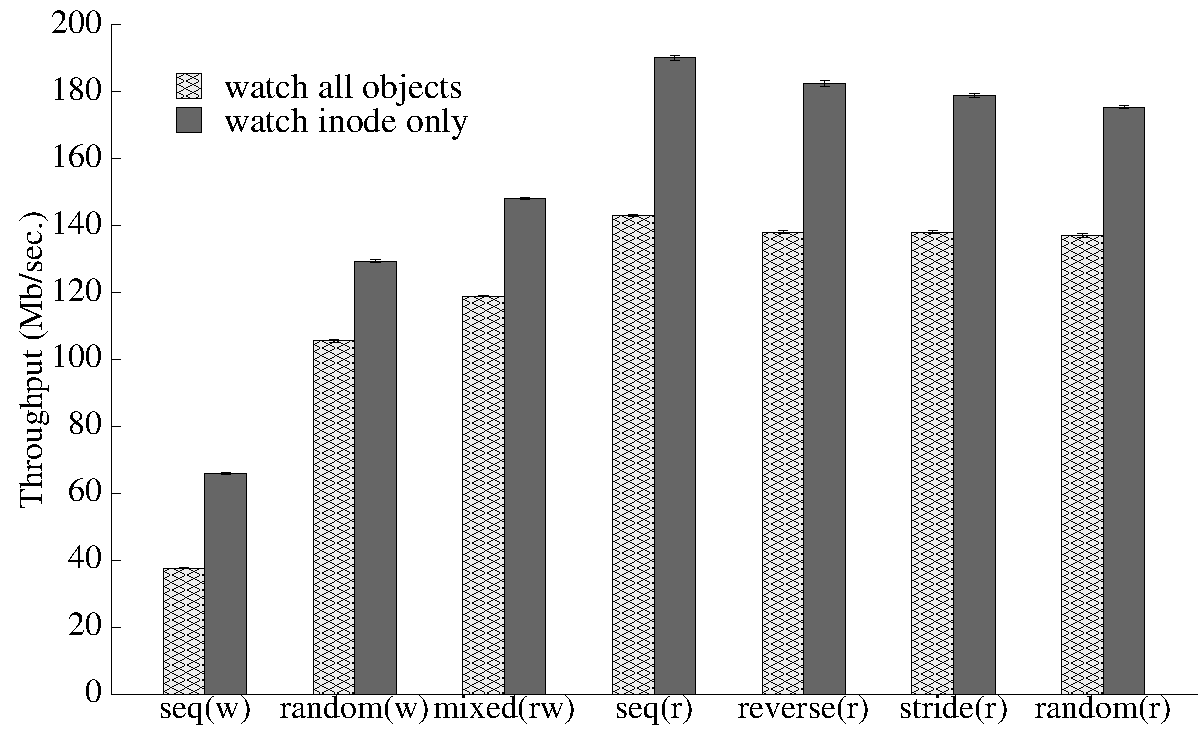
\includegraphics[width=6.0in]{thesis_watch_inode.pdf}
\end{center}
%\end{figure}

%\begin{figure}
\begin{center}
\vspace{1em}
\begin{tabular}{|l|r|r|}
  \hline
  \multicolumn{3}{|c|}{Watchpoint statistics for selective instrumentation in data centric instrumentation }  \\ \hline
  \hline
  & Watch \texttt{inode}s & Watch all \\
  \hline
  Number of basic blocks & 4217 & 5755\\
 % \hline
  Number of basic blocks with watched memory operations & 562 & 1479 \\
  \hline
  Number of executed basic blocks &  735367411 &  833167407 \\
  \hline
  Number of dynamic memory operations & 1519057148 & 1702295819 \\
  \hline
  Number of watched memory operators & 87433900 & 336149753 \\
  \hline
  Number of kernel hardware traps & 5522314 &  13403663 \\
  \hline
  Number of module hardware traps & 11234 & 112172 \\
  \hline
\end{tabular}
%\caption{\label{fig:watchpoint_inode_compare} Throughput in MB/sec of common file system operations and the watchpoint statistics when watchpoints are added selectively and only on \texttt{inode} objects.}
\caption[Performance impact of selective instrumentations for data-centric approach.]{\label{fig:watchpoint_inode}Throughput in MB/sec of common file system operations and the watchpoint statistics for data-centric instrumentation when watchpoints are added selectively and only for \texttt{inode} objects. The evaluation is done for transitive detach policy.}
%for the watched address is shown.}
\end{center}
\end{figure}


\Figref{watchpoint_performance} compares the overhead of code centric and data centric instrumentation. It shows that the code centric instrumentation performs better than the data centric instrumentation when all objects allocated by the module are watched. This is because the code centric instrumentation handles less hardware traps, which is costly and affects the performance of the system. Our evaluation compares the code centric instrumentation with the data centric instrumentation using transitive detach policy.


\begin{figure}[!h]
\begin{center}
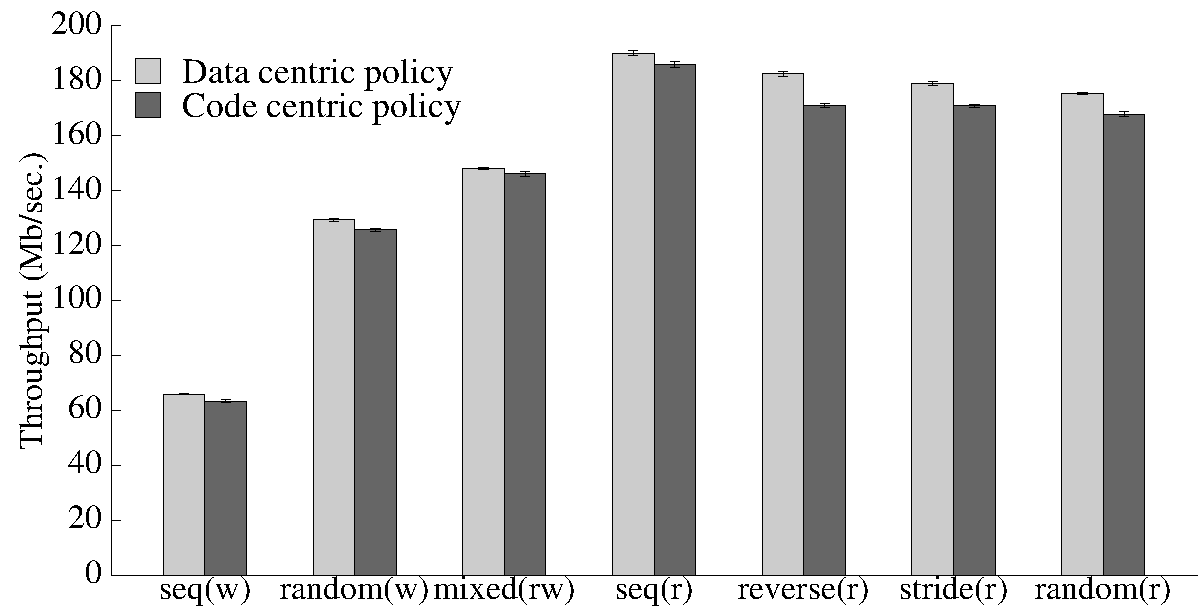
\includegraphics[width=6.0in]{thesis_watch_inode_compare.pdf}
\end{center}
%\caption{\label{fig:watchpoint_inode_compare}Throughput in MB/sec of common file system operations when watchpoints are added selectively and only for \texttt{inode} objects. The evaluation is done with transitive instrumentation policy.}
%for the watched address is shown.}
%\end{figure}  

%\begin{table*}
\begin{center}
\vspace{1em}
\begin{tabular}{|l|r|r|}
  \hline
  \multicolumn{3}{|c|}{Watchpoint statistics for selective instrumentation (watch \texttt{inode} objects)}  \\ \hline
  \hline
  & Code centric & Data centric \\
  \hline
  Number of basic blocks & 5405 & 4217 \\
 % \hline
  %Number of basic blocks with watched memory operations & 563 & 563 \\
  \hline
  Number of executed basic blocks &  814496751  & 735367411 \\
  \hline
  Number of dynamic memory operations & 1684738365 & 1519057148\\
  \hline
  Number of watched memory operators & 91699675 & 87433900 \\
  \hline
  Number of kernel hardware traps & 5446745 & 5522314 \\
  \hline
  Number of module hardware traps & 0 & 11234 \\
  \hline
\end{tabular}
\caption[Performance impact of selective instrumentations. The watchpoints are added on all file \texttt{inode} objects.]{\label{fig:watchpoint_inode_compare} Throughput in MB/sec of common file system operations and the watchpoint statistics when watchpoints are added selectively and only on \texttt{inode} objects.}
\end{center}
%\end{table*}
\end{figure}



\begin{figure}[!h]
\begin{center}
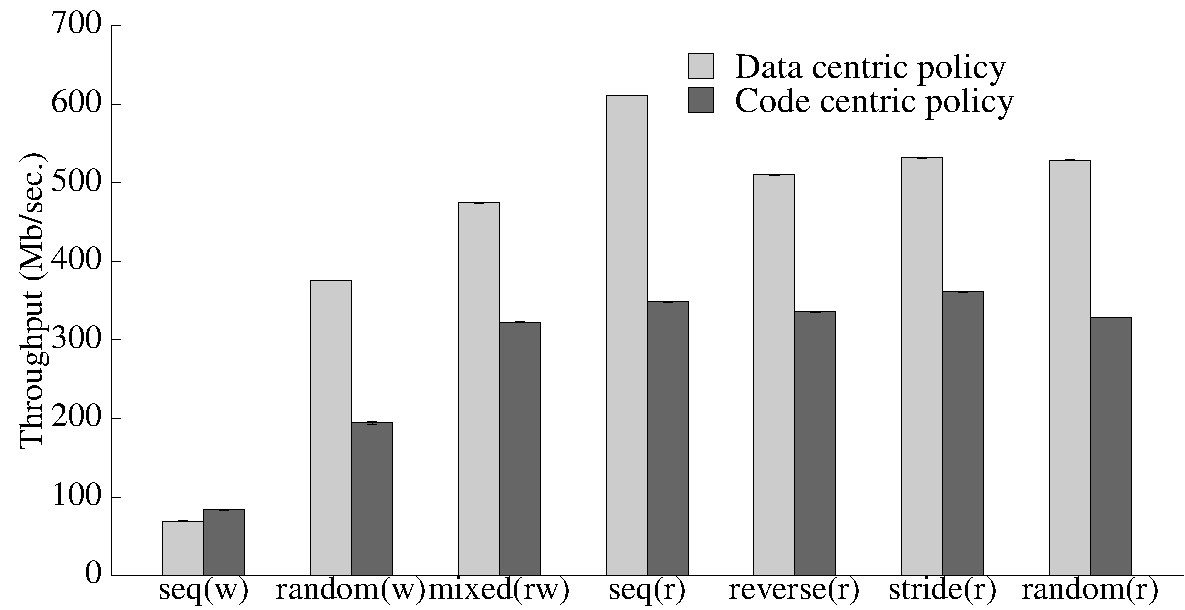
\includegraphics[width=6.0in]{thesis_selective_watch_no_inode.pdf}
\end{center}
\vspace{1em}
\begin{center}
\begin{tabular}{|l|r|r|}
  \hline
  \multicolumn{3}{|c|}{Watchpoint statistics for selective instrumentation (no hardware traps on kernel code)}  \\ \hline
  \hline
  & Code centric & Data centric \\
  \hline
  Number of basic blocks & 2259 & 1171 \\
  \hline
  Number of basic blocks with watched memory operations & 179 & 189 \\
  \hline
  Number of executed basic blocks &  238740476  & 105345884 \\
  \hline
  Number of dynamic memory operations & 568556578 & 221904835\\
  \hline
  Number of watched memory operators & 45649624 & 45637811\\
  \hline
  Number of module hardware traps & 0 & 10244480 \\
  \hline
\end{tabular}
\caption[Performance impact of selective instrumentations. The watchpoints are added on objects that are not getting accessed by the kernel code]{\label{fig:watchpoint_none_inode_compare} Throughput in MB/sec of common file I/O operations and the statistics of the watchpoint framework when watchpoints are added to the objects selectively which are not getting accessed by the kernel. This removes the effect of hardware traps from the code-centric instrumentations.}
\end{center}
%\end{table*}
\end{figure}
%on the throughput of file operations when only inode gets watched. In this case we used transitive policy for the evaluation.  

\paragraph{Selective instrumentation:}
The data centric approach enables selective instrumentation by adding watchpoints on selected objects. We first evaluated the performance of selective instrumentation by adding watchpoints only on file \texttt{inode} objects. \Figref{watchpoint_inode} shows the overhead of selective instrumentation and compares it with the overhead of data-centric instrumentation when all the module allocated objects are watched. Selective instrumentation performs better since it adds less watchpoints thus encountering fewer hardware traps, and executing fewer instrumented basic blocks.

We also compared the performance of selective instrumentation when using code-centric and data-centric approaches. \Figref{watchpoint_inode_compare} compares the overhead of selective instrumentation for both the approaches. It shows that selective instrumentation using data centric instrumentation has less overhead than with code centric instrumentation. This is because fewer basic blocks gets executed with data-centric instrumentation. The number of hardware traps encountered in both the approaches are also approximately same, causing similar overhead. 


The evaluation of code-centric approach shows that a major source of overhead in code-centric instrumentation comes due to adding watchpoints on file \texttt{inode} objects. These objects gets accessed mostly by the kernel code causing hardware traps. We removed the effect of these hardware traps from code-centric instrumentation by adding watchpoints selectively on the objects accessed only by the modules. We took the help of table~\ref{table:access_pattern_shared_objects} for adding watchpoints on the objects selectively.

 \Figref{watchpoint_none_inode_compare} represents the overhead of selective instrumentations for data-centric approach and compares it with the code-centric instrumentation. It shows that the selective instrumentation reduces the overhead of using the watchpoint framework to {\texttildelow}5\% where as the baseline instrumentation for code-centric approach causes an overhead of {\texttildelow}40\%. This is because the selective instrumentation executes less number of basic blocks ({\texttildelow}2.3{\footnotesize$\times$}). The evaluation also shows that the performance of sequential write operation in case of data-centric approach is less than the code-centric. We analyzed the behavioral of write operations and found that {\texttildelow}50\% of the total hardware traps was only happening during sequential write operations. This could be a reason of sequential write not performing better.    

 The evaluation of both, the code-centric and data-centric approaches for implementing behavioral watchpoints, shows an interesting trade-off between the amount of instrumented code executed from the code-cache and how much of that code actually needs to be instrumented. The code-centric approach always suffers from the overhead of baseline instrumentation since it always executes instrumented basic block from code cache. The data-centric instrumentation overcome this by adding instrumentation on-demand. However, it suffers from the high cost of the hardware traps which triggers the instrumentation. The number of executed basic blocks also increases with the hardware traps which causes additional overhead.

 We also saw that the number of hardware traps depend on the type of the watched objects. Adding watchpoints on frequently accessed shared objects such as file \texttt{inode}s, causes a large number of traps affecting the performance of the watchpoint framework where as watching relatively less accessed objects such as \texttt{ext3\_block\_alloc\_info} causes less traps improving the performance of the data-centric instrumentation.

 The advantages and disadvantaged of both the approaches opens up the space to further explore the possibility of switching between the two approaches at runtime. This will reduce both the overhead of baseline instrumentation and the cost of hardware traps, thus improving the performance of the system. The evaluation of code-centric instrumentation also shows its need to provide the whole kernel instrumentation support. We plan to take this as an immediate future work.

 %The evaluation of the watchpoint framework using \emph{iozone} shows the


 %It shows that the selective instrumentation using data-centric approach reduces the overhead of using the watchpoint framework 


 %for both the code-centric and data-centric approaches.



 %by adding watchpoints on such objects. The data centric instrumentation in such case performs much better than the code centric approach and the performance of data centric instrumentation is close to that of the native system. 


%and added watchpoints selectively on objects which does not get accessed by the kernel.


%, we saw that a major source of overhead in code centric approach is the number of hardware traps. Much of these hardware traps occur due to adding watchpoints on \texttt{inode} objects and the code centric instrumentation was performing worse when it was getting watched. To remove the effect of hardware traps in selective instrumentation, we took the help of table~\ref{table:access_pattern_shared_objects} and added watchpoints selectively on objects which does not get accessed by the kernel. \Figref{watchpoint_none_inode_compare} compares the overhead of selective instrumentations by adding watchpoints on such objects. The data centric instrumentation in such case performs much better than the code centric approach and the performance of data centric instrumentation is close to that of the native system. 

%the number of instrumented basic block executed in case of data-centric approach is less than the code-centric approach. 
%However, it also shows that there are more hardware traps encountered with data-centric approach.

%The watchpoint gets added to the objects selectively. We evaluated the performance of selective instrumentation by adding watchpoints only to the \texttt{inode}s. \Figref{watchpoint_inode} compares the overhead on the throughput of file operations when only inode gets watched. In this case we used transitive policy for the evaluation.   
% the overhead of code-centric and data-centric approach 

%using complete data-centric approach.



%from providing the complete data-centric approach by wrapping all the function pointers at the interface for faster attach and detach.

%and we also used the same experimental setup for running the benchmark. We also disabled the wrappers for fast attach and detach since it prohibits the framework from providing the complete data-centric approach by wrapping all the function pointers at the interface for faster attach and detach.


%\subsection{Filebench}
%We evaluated the real workload using Filebench file system benchmark.

\subsection{Macrobenchmark}
We further evaluated the overhead of the behavioral watchpoint framework using a file system macrobenchmark consisting common system utilities. We used the same experimental setup and mounted the \texttt{ext3} module on a RAMDisk of size 1GB. The macrobenchmark operated on the Linux source tree (\texttt{linux-3.2.50}). Table~\ref{table:system_utils-benchmark} shows the overhead of behavioral watchpoints on the standard system utilities. For both the code-centric and data-centric approaches, the framework adds watchpoints selectively on all \texttt{inode} objects allocated from the look-aside buffer. The evaluation shows data-centric instrumentation is performing better than code-centric instrumentation when used for watching objects selectively all the \texttt{inode} objects.


\begin{table*}
\begin{center}
\vspace{1em}
\begin{tabular}{|l|r|r|r|}
  \hline
   & Native execution & Data centric approach & Code centric approach \\
  \hline
  cp & 6.64 & 10.82 & 11.61\\
  \hline
  tar & 2.64 & 3.84 & 4.16\\
  \hline
  stat & 3.90 & 5.12 & 5.44\\
  \hline
  grep & 3.94 & 5.36 & 5.54\\
  \hline
\end{tabular}
\caption[Performance impact of the watchpoint framework on macrobenchmark]{\label{table:system_utils-benchmark}The CPU (system \& user) time for the standard system utilities performing file system operations on a RAMDisk of size 1GB. The framework adds watchpoints selectively on all \texttt{inode} objects of the \texttt{ext3} module.}
\end{center}
\end{table*}


\begin{figure*}[t!]
\begin{multicols}{2}
\begin{center}
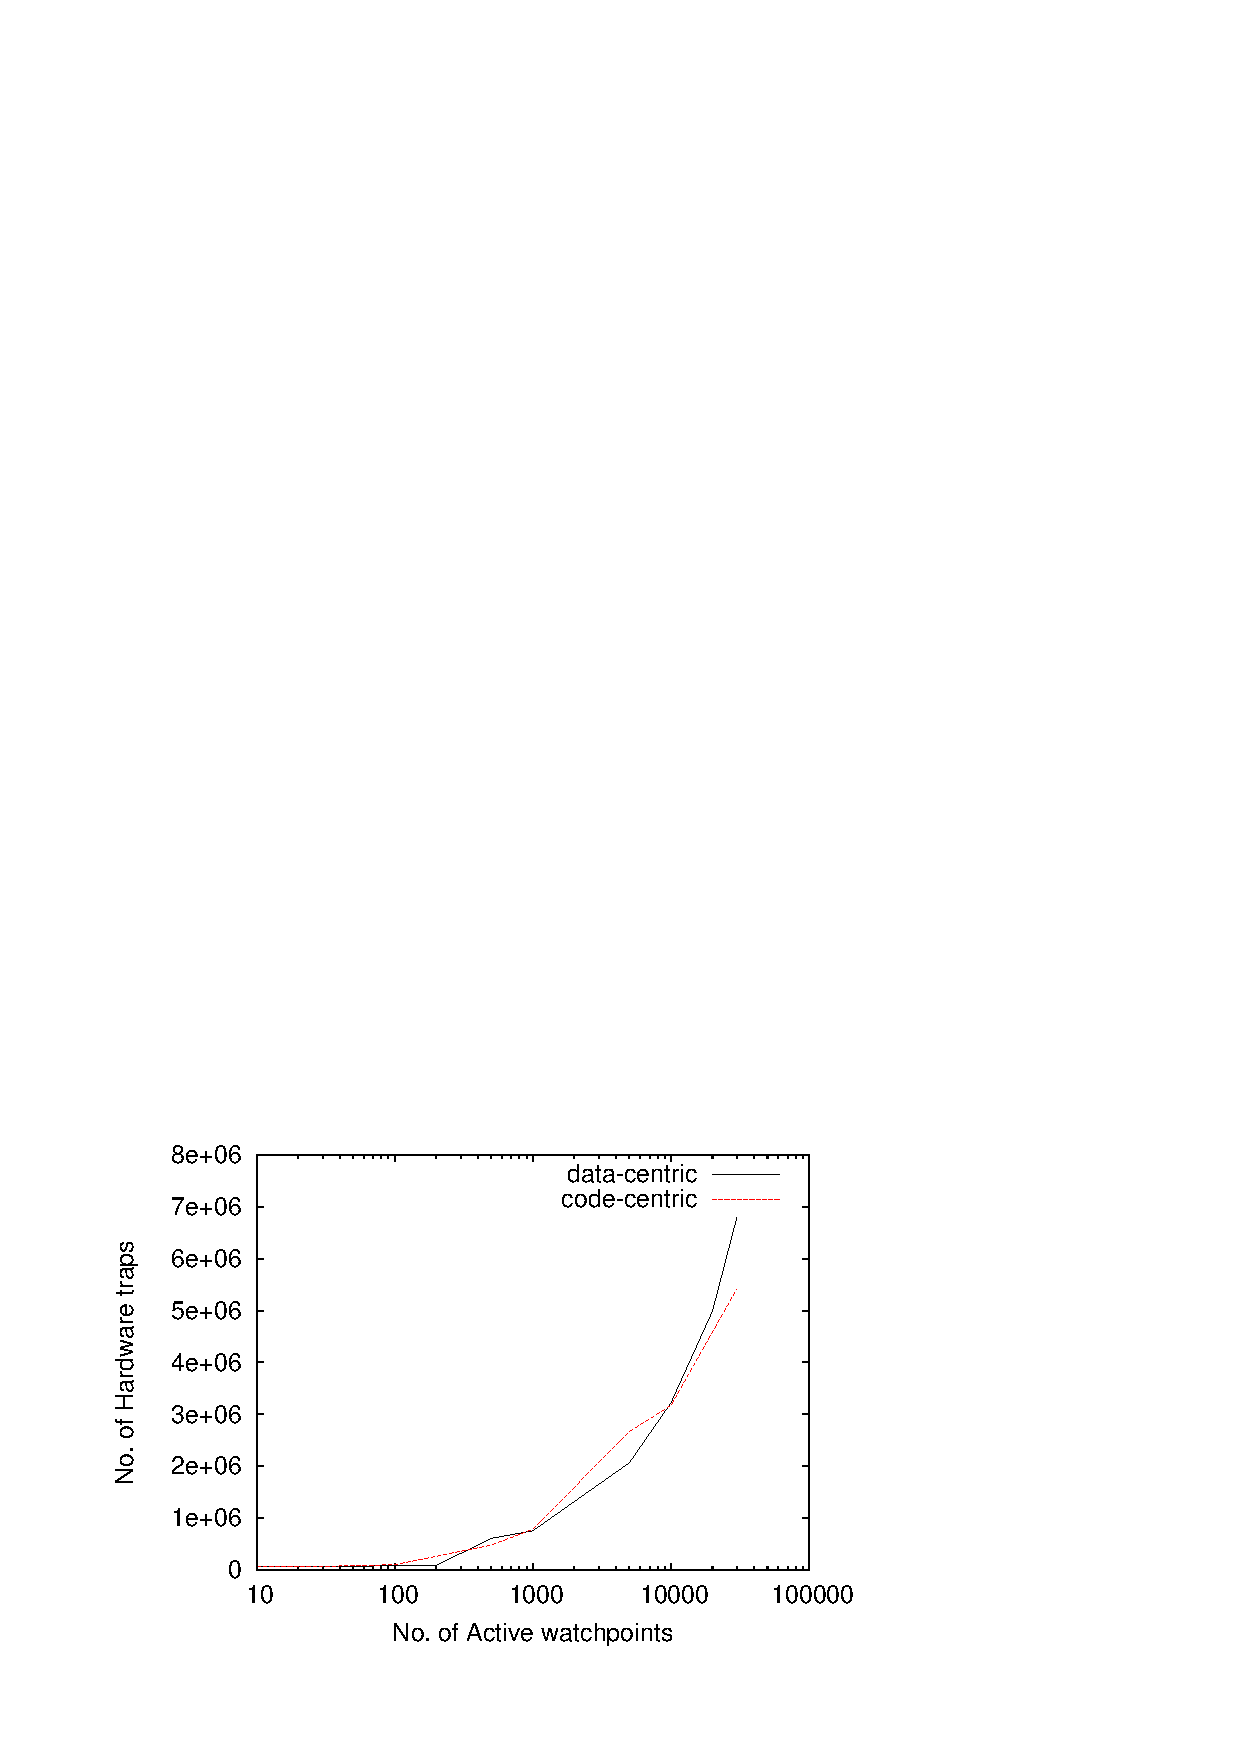
\includegraphics[width=3.5in]{hardware_traps.pdf}
\end{center}
\columnbreak
\begin{center}
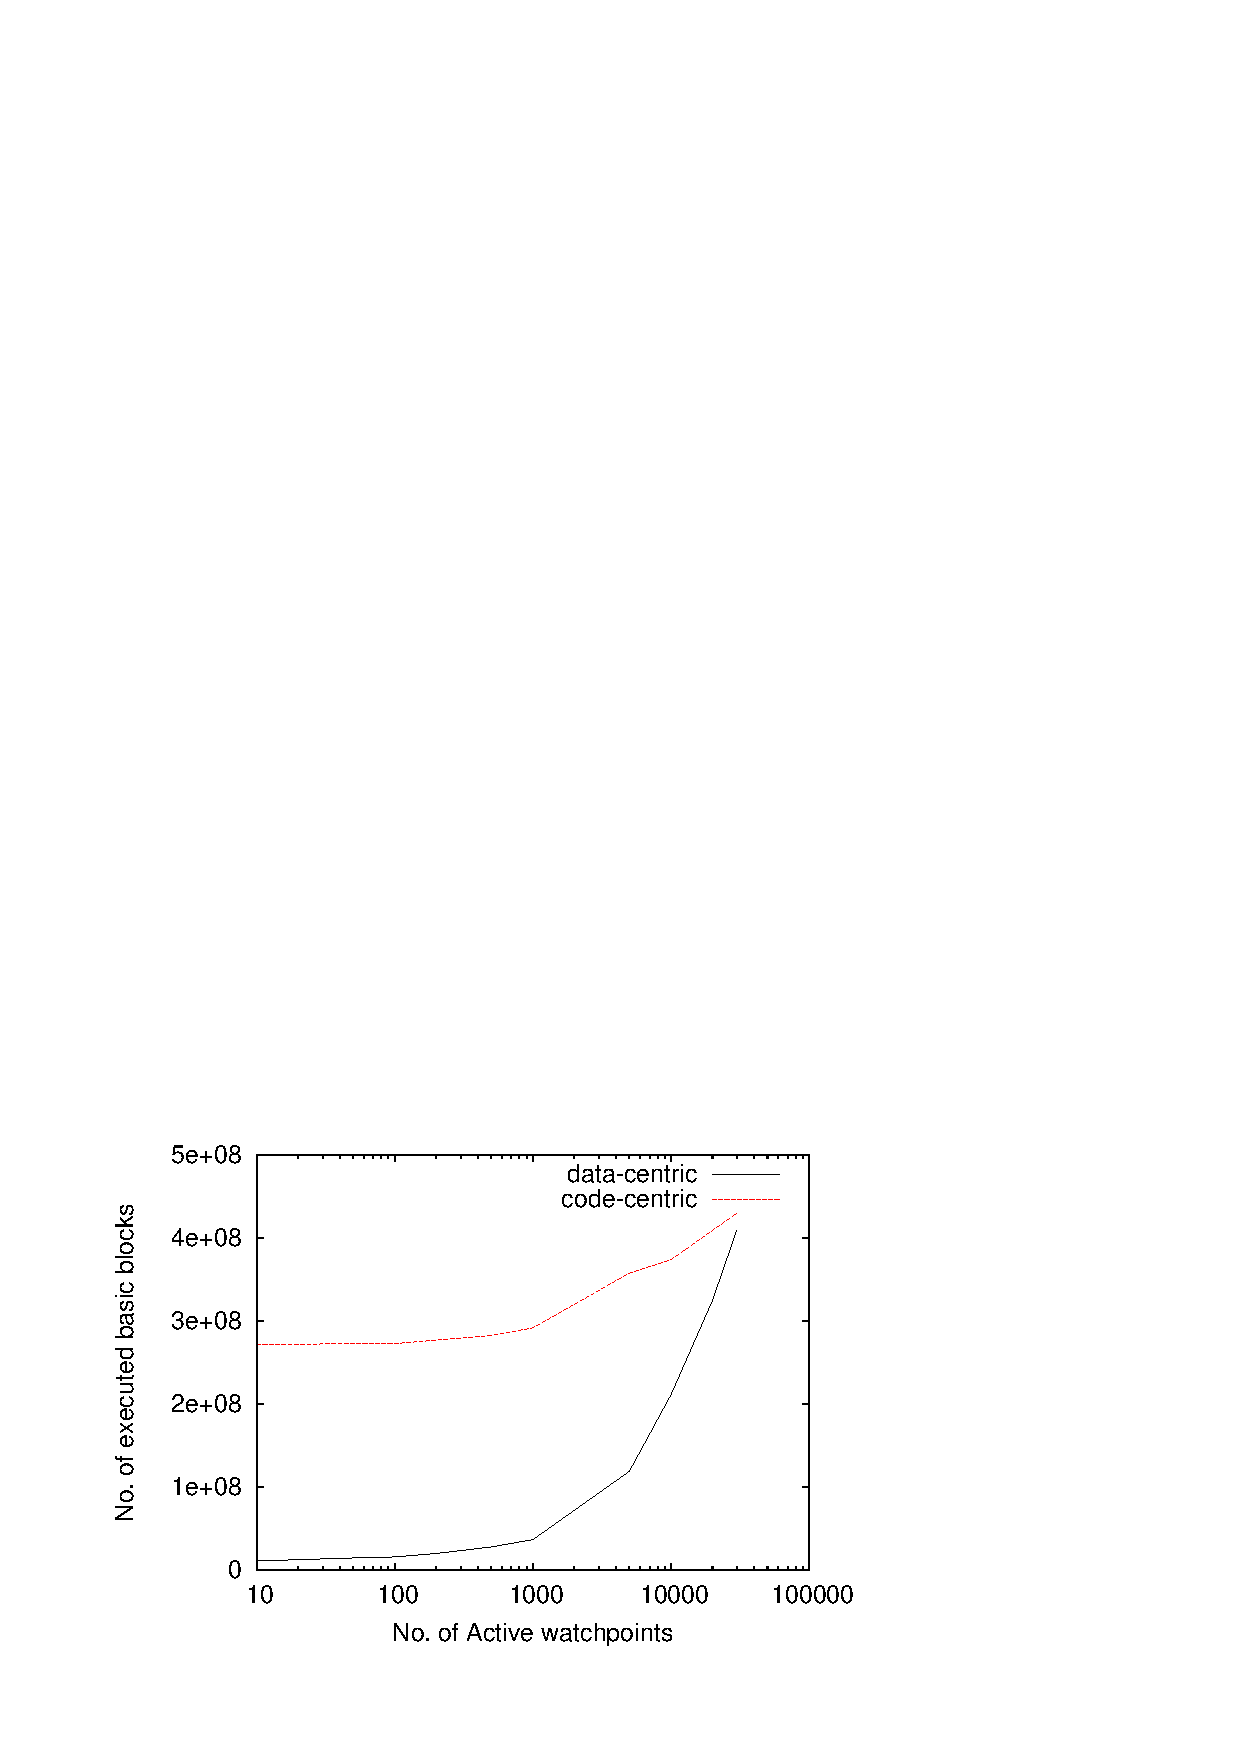
\includegraphics[width=3.5in]{executed_bb_data.pdf}
\end{center}
\end{multicols}
\caption[Cost profile of the watchpoint framework in terms of number of added watchpoints.]{\label{fig:traps_profile}The changes in the number of hardware traps and the number of executed basic blocks with the changes in number of added watchpoints.}
\end{figure*}

In both the code-centric and data centric approaches, the major factors which affects the performance are the number of basic block executed and the number of hardware traps encountered during the execution. We also used microbenchmark to study the changes in the number of hardware traps and the basic block executed with the change in the number of watchpoints. \Figref{traps_profile} shows that both the code centric instrumentation and data centric instrumentation encounters same number of hardware traps. This is because we add watchpoints selectively on all \texttt{inode} objects which gets accessed both by the module and the kernel code equally causing hardware traps. We also see fewer occurrences where the number of traps in case of data centric is less than the code centric instrumentation. One reason for this could be that the code centric instrumentation always detaches itself at the interface where as the data centric instrumentation, with transitive detach policy, does not always detaches itself at the interface.

\Figref{traps_profile} also shows that with fewer watchpoints the code centric instrumentation still executes many more basic blocks than the data centric approach. This causes increased overhead for code centric instrumentation even when fewer watchpoints are added. 




% and causes more overhead even when the 


% We also discussed previously that data centric instrumentation is useful when watchpoints are added on objects 

\begin{table*}
\begin{center}
\vspace{1em}
\begin{tabular}{|l|l|l|}
  \hline
   Workload & Setting & Data Size \\
  \hline
  Fileserver & nfiles=10K & 1.2GB \\
  \hline
  Webserver & nfiles=1K, & 14.76MB \\
  \hline
  Webproxy & nfiles=10K & 154MB \\
  \hline
  Varmail & nfiles=1K & 14.76MB \\
  \hline
\end{tabular}
\caption[Filebench server benchmark workload characteristics.]{\label{table:filebench-benchmark}Benchmark characteristics.}
\end{center}
\end{table*}


\begin{figure}[!h]
\begin{center}
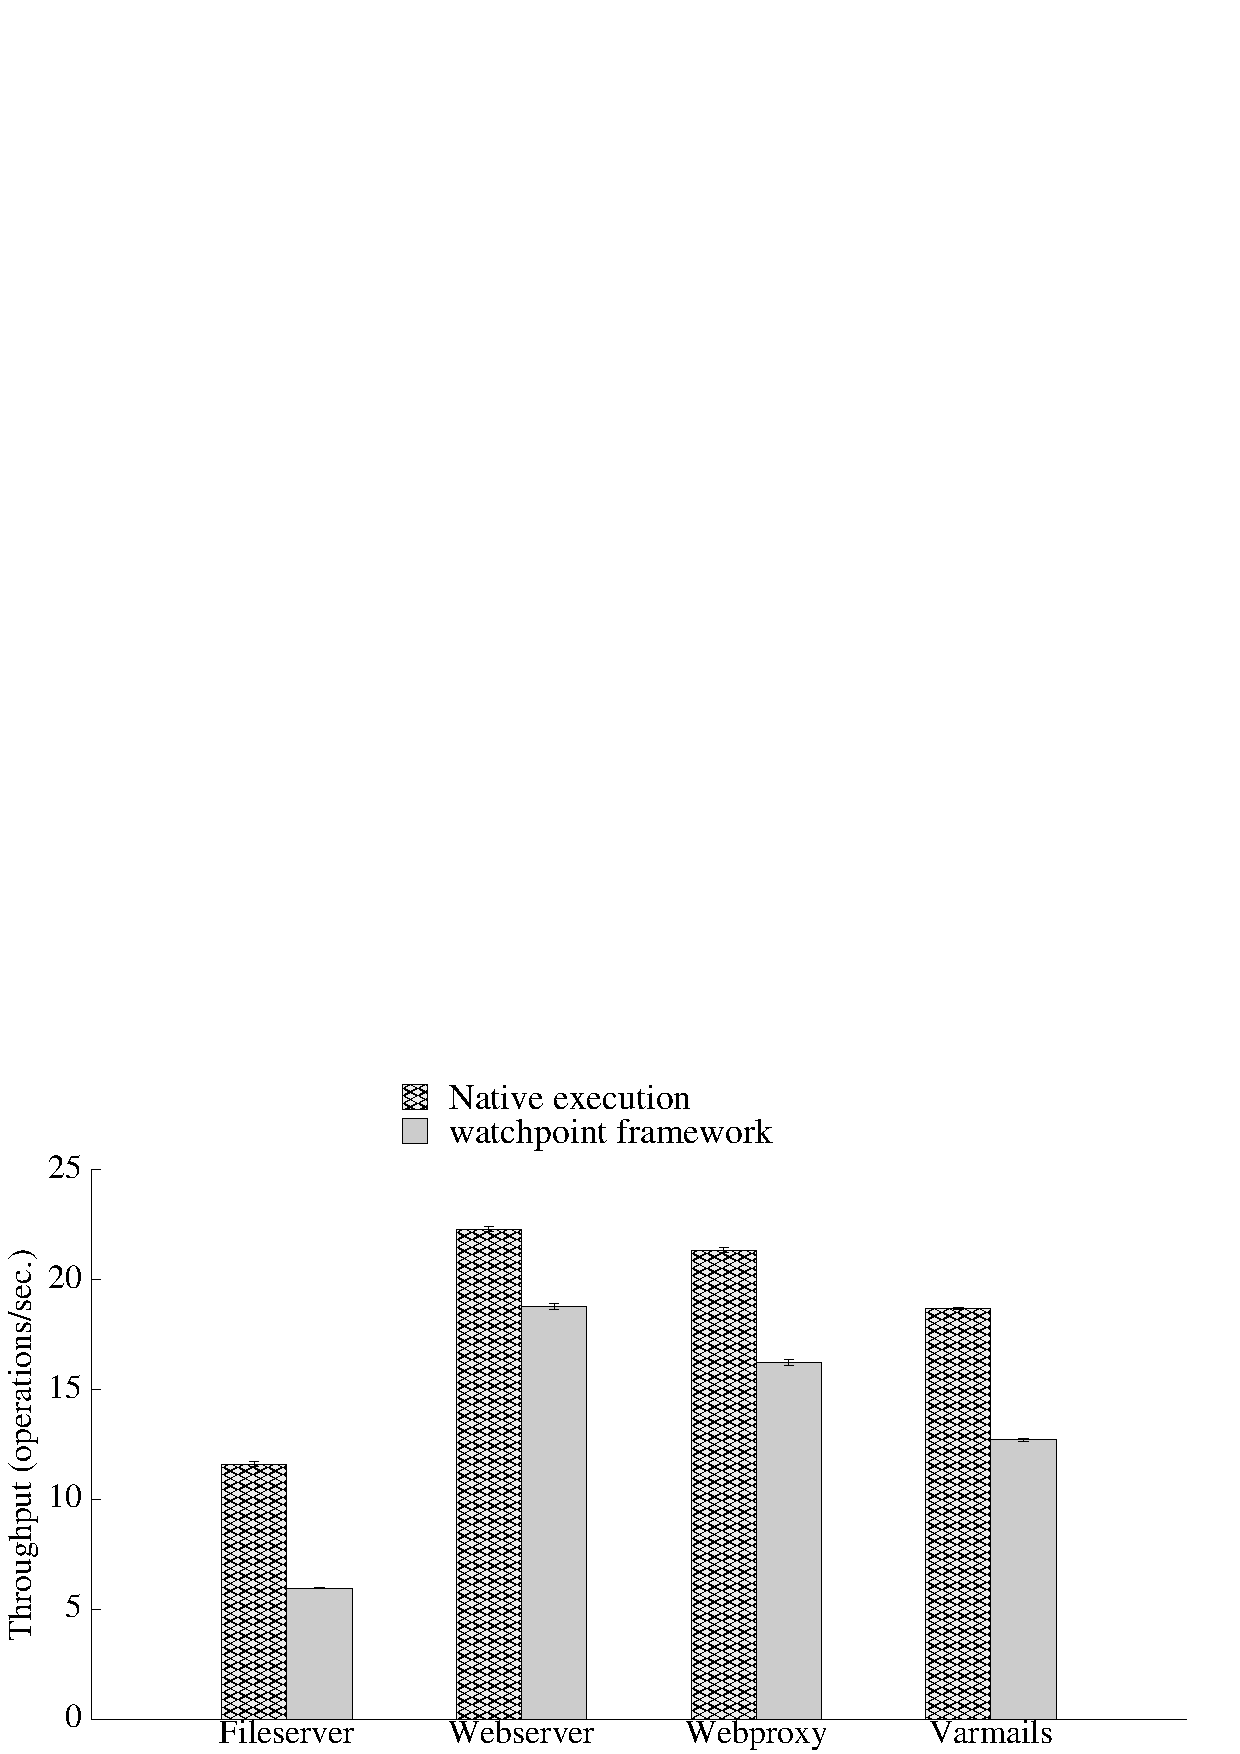
\includegraphics[width=6.0in]{filebench.pdf}
\end{center}
\caption[Performance impact of the watchpoint framework on Filebench server benchmark workloads.]{\label{fig:sever_performance}Throughput in file system operations/sec for the filebench workload personalities shown in Table~\ref{table:filebench-benchmark}.}
%for the watched address is shown.}
\end{figure}




\subsection{Server Benchmark}
We used the Linux port of Filebench version 1.4.9, with four of the standard server workload personalities, to evaluate the watchpoint framework. We used the same experimental setup as with the \emph{iozone} and enabled default settings to define the workload characteristics. The relevant characteristics for the workloads are shown in Table~\ref{table:filebench-benchmark}. With the default characteristics, the datasets easily fit in the RAMDisk used for evaluation. This does not limit the workload with the performance of I/O operations.

\Figref{sever_performance} shows the throughput of the different Filebench server workloads. For evaluation we used data-centric instrumentation with all file \texttt{inode} objects getting watched. The data centric instrumentation reduces the throughput for all the workload personalities by ~40\%. We also evaluated the code-centric instrumentation using Filebench and noticed similar drop in the throughput but we are not showing it here.

%Null Client reduces
%throughput by 3X for fileserver, and by 4.5X and 4.2X for webserver
%and webproxy, respectively. There is only a small additional
%reduction in throughput with Instruction Count. We can see that
%the drop in throughput is correlated with the number of threads
%used in the workload, with webserver and webproxy both using
%100 threads. The overhead for varmail, which syncs its data to disk
%frequently, is much lower, with only a 1.4X drop in throughput.

%We also evaluated the performance of behavioral watchpoints using real workloads. We mounted \texttt{ext3} file system module on a disk of size 20GB and used Filebench to simulate the real workloads. Table~\ref{table:filebench-benchmark} shows the characteristics of the workload we used for the evaluation.


%We used same experimental setup and mounted \texttt{ext3} module on RAMDisk of size 1GB. The macrobenchmark operated on the source tree of \texttt{linux-3.2.50} branch. We used the following five benchmarks to evaluate the performance overhead of the watchpoint framework: 

%\begin{enumerate}
%	\item \emph{MakeDir:} It reads the directories subtree of source program and constructs the identical target directories subtree. It uses \texttt{mkdir} utility for creating the directories recursively.
%	\item \emph{Copy:} It copies all the files from source files subtree to the target files subtree. We used \texttt{rsync} command to copy the files from the source directory to the target directory.
%	\item \emph{ScanDir:} It recursively goes to all the files in target directory and performs the stat operation on each file.
%	\item \emph{ReadAll:} It reads every byte of the every file in the target directory.
%	\item \emph{Compile:} It compiles and links all the files for the source program.
%\end{enumerate}


%Behavioral watchpoints uses non-canonical address to add watchpoints with the allocated objects. This provides the opportunity to implement data-centric instrumentation. Data-centric instrumentation is particularly important when watchpoints are unlikely to be triggered. We implemented three different policy for data-centric instrumentation: i) transitive policy, ii) function-only policy and iii) basic block policy. The details about it is provided in section. 

%Data-centric instrumentation also uses three different instrumentation policies and the details of which is provided in section.
%We used \emph{iozone} to evaluate the performance of data-centric instrumentation and we also used the same experimental setup for running the benchmark. We also disabled the wrappers for fast attach and detach since it prohibits the framework from providing the complete data-centric approach by wrapping all the function pointers at the interface for faster attach and detach.

%In this experiment, We studied the effect of hardware exceptions and watchpoint instrumentation overhead on the performance of filesystem throughput. We used the three data-centric policies for the evaluation and compared their performance in terms of the number of hardware exception encountered and the number of instrumented basic block executed. 

%Figure~\ref{fig:watchpoint_performance_data_driven} shows the throughput of common filesystem operations for data-centric instrumentation approach. Table~\ref{table:data-centric-table} shows the number of traps encountered along with the number of executed basic block and number of memory operations performed. The evaluation result shows the performance decrease with the number of traps but it gets compensated by executing less number of basic blocks and performing less number of memory operation which has an additional cost of watchpoint instrumentation.

% We also evaluated the number of hardware exception encountered and the number of basic block executed for each policies.



 %We also varies the number of watchpoints to see how the cost of data-centric instrumentation varies with the number of added watchpoints.


%These allocated objects when gets accessed causes hardware exceptions or traps. Behavioral watchpoint framework uses this to implement watchpoint instrumentation on trap. This approach allows selective instrumentation and can take advantage of low overhead when watchpoints are unlikely to be triggered. The trap-based instrumentation approach uses three different instrumentation policy: policy 1 includes the transitive instrumentation where the framework attaches itself on trap and instruments till it finds the indirect call or return and detaches itself. Policy 2 instruments the body of the function which encounters the trap and changes policy to go native on call and return. Policy 3 is the most conservative policy and tries to instruments minimum of the code. The instrumentation framework attaches itself on trap and detaches and goes to native execution on any control transfer, instrumenting only single basic block at a time. We evaluated all the three instrumentation policy by running the \emph{Iozone}~\cite{citeulike:919086} and studying the throughput of common file system operations. In trap-based instrumentation approach behavioral watchpoint is implemented on trap. We also used microbenchmark to evaluate the cost of taking trap and studied how the number of these traps increases over different policy and affects the performance.







%One of the important feature of data-driven instrumentation is the ability to watch objects selectively. The selective addition of watchpoints will have less instrumentation cost and also the number of hardware exception encountered will be less. We evaluated the performance of selective instrumentation by adding watchpoints to only \texttt{inode} objects. Figure~\ref{fig:watchpoint_inode} the overhead when only inode gets watched and compares it with everything watched. However the selective instrumentation of objects may suffer from the cold code-cache effect and it can cause high overhead.


%We also studied the change in throughput of file operations for data-driven instrumentation with the increase in number of watchpoints. With the increase in the number of watchpoints the number of executed basic block and hardware traps increases. Figure shows how the throughput decreases with the increase in number of watchpoints.


%\subsubsection{Iozone}
%In our experimental setup, the \texttt{ext3} filesystem was mounted on a 1GB RAMDisk (mounting loads the \texttt{ext3} and \texttt{jbd} journaling kernel modules). IOzone creates two processes (reader, writer) performing common file operations on a file of size 480Mb with a record size of 1Kb. Watchpoints were added to addresses returned by the two most-used allocators in \texttt{ext3} and \texttt{jbd}: \texttt{\_\_kmalloc} and \texttt{kmem\_cache\_alloc}. \Figref{iozone-workload-overhead} shows the drop in throughput of filesystem operations when using the watchpoints instrumentation; \emph{watchpoint\_null} represents the overhead of baseline watchpoints instrumentation with no added watchpoints, and \emph{watchpoint\_watched} shows the overhead where module-allocated objects are watched. \Figref{iozone-workload-overhead} also shows the overhead of the heap-allocated buffer overflow detector using behavioral watchpoints. Our implementation of the buffer-overflow detector does not yet use various optimizations offered by Granary at the instrumentation and wrapper layer, and thus exhibits high overhead.

%\subsubsection{File operations}



%\paragraph{Code-centric Vs Data-centric Instrumentation}
%We also compared the performance of Code-centric and Trap-based instrumentation approach by running them under best case and worse case scenarios. We used Iozone as the filesystem benchmark and used the similar experimental setup for running filesystem module \texttt{ext3}. Trivially the best case is when there are no watchpoints. To evaluate the worse case we add watchpoints with every allocated memory blocks while Iozone. During the experiment the total number of allocations done by \texttt{ext3} module was ~2500. 


%\begin{table*}
%\begin{center}
%\caption{Performance of macrobenchmark}
%\begin{tabular}{ |c|c|r|r|r| }
%\hline
%\multicolumn{5}{ |c| }{Performance of Synthetic Macrobenchmark} \\
%\hline
%\hline
%Macrobenchmarks & time &Native & Data-centric & Code-centric\\ \hline
%\multirow{3}{*}{MakeDir} & user & 0.07 & 0.06 & 0.05 \\ \cline{2-5}
% & sys & 0.13 & 0.08 & 0.08\\ \cline{2-5}
% & real & 1.28 & 0.73 & 0.73\\ \hline
% \hline
%\multirow{3}{*}{Copy}& user & 3.03 & 0.09  & 0.20\\ \cline{2-5}
% & sys & 6.25 & 9.70 & 10.42\\ \cline{2-5}
% & real & 26.35 & 26.45 & 36.66\\ \hline
% \hline
%\multirow{3}{*}{ScanDir} & user & 3.44 & 0.0 & 0.0\\ \cline{2-5}
% & sys & 2.62 & 0.0 & 0.0\\ \cline{2-5}
% & real & 43.10 & 0.0 & 0.0\\ \cline{2-5}
% \hline
% \hline
%\multirow{3}{*}{ReadAll} & user & 2.73 & 0.0 & 0.0\\ \cline{2-5}
% & sys & 2.46 & 0.0 & 0.0\\  \cline{2-5}
% & real & 22.64 & 0.0 & 0.0\\ \cline{2-5}
%\hline
%\hline
%\multirow{3}{*}{Compile} & user & 551.59 & 0.0 & 0.0\\ \cline{2-5}
% & sys & 49.78 & 0.0 & 0.0\\  \cline{2-5}
% & real & 651.30 & 0.0 & 0.0\\ \cline{2-5}
%\hline
%\end{tabular}
%\label{table:compile-benchmark}
%\end{center}
%\end{table*}

%\subsection{Macrobenchmark}
%We further evaluated the performance of behavioral watchpoint framework with the synthetic macrobenchmark representing the real-world workloads. The benchmark uses different system utility functions and operates on a directory subtree containing the source code of a program. The experimental setup was same and we used \texttt{linux-3.2.50} source code for the analysis. The details about the program source code if provided in table. We used following five benchmarks to evaluate the system:  

%We created the synthetic benchmark with the reference of Andrew File system benchmark and it perform the following five basic file system operations.
%\begin{enumerate}
%	\item \emph{MakeDir:} It reads the directories subtree of source program and constructs the identical target directories subtree. It uses \texttt{mkdir} utility for creating the directories recursively.
%	\item \emph{Copy:} It copies all the files from source files subtree to the target files subtree. We used \texttt{rsync} command to copy the files from the source directory to the target directory.
%	\item \emph{ScanDir:} It recursively goes to all the files in target directory and performs the stat operation on each file.
%	\item \emph{ReadAll:} It reads every byte of the every file in the target directory.
%	\item \emph{Compile:} It compiles and links all the files for the source program.
%\end{enumerate}

%We used RAMdisk mounted with \texttt{ext3} filesystem as the target directory. For Compile benchmark, we used similar configuration across all builds. We modified the default configuration to remove the loadable module from the build process and we calculated the time for configuration and compilation separately. The result only shows the CPU time for compilation phase. We also used \texttt{strace} to trace the system calls during the build process. Table~\ref{table:compile-benchmark} shows moderate overhead of Granary and behavioral watchpoints with the increase in \texttt{cpu} time.
%Table~\ref{table:compile-benchmark} shows the performance of the synthetic macrobenchmarks. We run these benchmarks on the vanilla Linux kernel version 3.2.50. The details about the kernel source code is given in table.


%For running the benchmark we used Ramdisk mounted with \texttt{ext3} module as the target subtree directory. We created the benchmark to be CPU bound



%\chapter{Approach}\label{sec:appr}
%Behavioral watchpoint provides an efficient software-based watchpoint framework that simplifies the implementation of DBT-based program analysis and debugging tools. This chapter describes the design of behavioral watchpoints and the various features enabled by our design. We present the challenges raised by our approach and then describe our implementation of behavioral watchpoints. 
%Behavioral watchpoint leverages the advances in binary instrumentation and code manipulation tool to provide an efficient debugging framework that can substantially increase the feature set of standard off the shelf debuggers. 
Two characteristics that defines the watchpoints are:
\begin{enumerate}[i)]
	\item Context-specific information is embedded in each watchpoint. This information is directly available when a watched address is accessed, providing significant versatility in monitoring a large number of memory addresses.
	%\item The action taken when a watched address is accessed is a component of the context-specific information. This implies that different watchpoints can \emph{behave} differently.
	\item A behavioral watchpoint watches a \emph{range} of addresses, enabling object-granularity watchpoints, i.e., one watchpoint can watch an entire object or memory block.
%watchpoints. This enables the feature where one watchpoint can watch the entire object or memory block.%(i.e., one watchpoint watches an entire object). 
\end{enumerate}



%. This design supports our goal of allowing one watchpoint to monitor all memory accesses to a single object.

%To achieve this design goal, we implemented
\section{Design}\label{sec:design}
The design of the behavioral watchpoint framework is motivated by our aim to provide context-specific information on memory accesses, which helps provide significant versatility when monitoring these accesses. This context specific information is stored in an in-memory data structure and accessed before memory read/write operations. %which is referred before every read/write operations on memory blocks. and accessed before memory read/write operations. 
%
%
Our design is based on the key observation that the pointers in 64 bit architectures have spare bits. Both AMD64 and Intel x86-64 processors use a 48 bit implementation leaving 16 spare bits that can be used to store pointer metadata information. 
%which can be used to store the information about the pointers.

We implement watchpoints by adding an extra level of indirection to memory addresses. An unwatched address is converted into a watched address by changing its spare high-order bits. The high order bits of an unwatched address have the value \texttt{0xffff}. We call this value the canonical value. For watched addresses, the high-order bits are converted to a non-canonical value that helps identify context-specific information about the range of memory being watched. This information, called the watchpoint's \emph{descriptor}, contains the originating watched address, meta-information and a set of functions (\emph{vtable}) to invoke when watched memory is dereferenced. Since watchpoint information is embedded in the high-order bits, a typical offset of a watched address is another watched address that shares the same descriptor. 

The design of behavioral watchpoints is shown in \Figref{watchpoint_descriptor_table}. Our design uses 15 high-order bits (called the \emph{counter index}) and an additional 8 bits (bits 20-27, called the \emph{inherited index}) of a watched address to identify the index into a global \emph{watchpoint descriptor table}. The \emph{watchpoint descriptor table} stores a pointer to the watchpoint's descriptor. The key advantage of our design scheme is i) the ability to map watched addresses to unwatched addresses using a simple bitmask and  ii) the ability to easily access a watchpoint's descriptor when a watched address is accessed. The high-order 15 bits counter index allows us to use 32K watchpoints at a time and the additional 8 bits of inherited index extends the number of possible watchpoints to 8M. The inherited index is left unchanged when converting an unwatched address into watched.

However, one drawback of our design is that an offset of a watched address can cause the low-order bits to overflow into the inherited index and this will lead a watched address to point to an incorrect descriptor. One approach to deal with this issue is to assign  multiple descriptors for the watched objects holding the same meta-information and putting them in adjacent indices or duplicating the same descriptor entry across adjacent indices. This is possible because inherited indexes make the descriptor table more sparse allowing them to have duplicate entries.


%15 bits only allows 32K watchpoints. To increase the number of watchpoints, we use
%an additional 8 bits (bits 20-27, called the counter index)
%in the address to index into the watchpoint descriptor table (Figure 1). This counter index  and is left unchanged when
%converting an unwatched address into a watched address.
%The key advantage of our watchpoint scheme is the ability to directly map watched addresses to unwatched addresses using a simple bitmask. The main drawback of
%the scheme is that an offset of a watched address can  


%e 48 out of 64 bits in pointers,
%and Windows further limit this to 43 bits for user space
%programs. Thus 21 bits in the pointer representation are
%not used. Next we describe two uses for these spare bits,
%and present a performance evaluation on AMD64.

%Behavioral watchpoints is designed by adding an extra level of indirection to memory addresses. An unwatched address is converted into a watched address by changing its high-order bits. These high-order bits indirectly identify context-specific information about the range of memory being watched. This information, called the watchpoint's \emph{descriptor}, contains the originating watched address, meta-information and a set of functions (\emph{vtable}) to invoke when watched memory is dereferenced. Since watchpoint information is embedded in the high-order bits, a typical offset of a watched address is another watched address that shares the same descriptor. 

\begin{figure}[t]
\begin{center}
%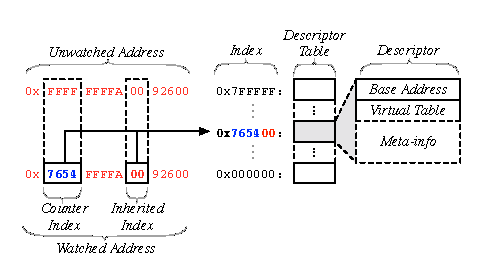
\epsfig{file=watchpoints.eps, width=3.0in, height=1.4in}
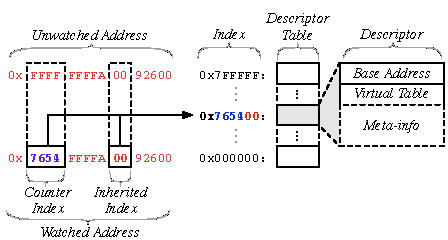
\includegraphics[width=6.0in]{watchpoints.pdf}
\end{center}
\vspace{-15pt}
\caption[Design of behavioral watchpoints.]{\label{fig:watchpoint_descriptor_table}A watched address (bottom left) and its corresponding unwatched address (top left) are compared. The watched address takes the form of non-canonical address that are not addressable in kernel space. The watchpoint framework uses a \emph{counter index} and an \emph{inherited index} to store the descriptor information in a global descriptor table. The process of resolving the watchpoint descriptor is shown.}
%for the watched address is shown.}
\end{figure}


Our design of behavioral watchpoints is geared to the 64 bit x86 (x86-64) architecture. In kernel space on the x86-64 architecture, the addressable memory includes the canonical form of addresses with their 16 high-order bits set to 1. Tagging these higher order bits with the descriptor information converts them to a non-canonical address that triggers a hardware exception when dereferenced. The watchpoint framework takes advantage of the exception to implement behavioral watchpoints.

%The design of behavioral watchpoint is shown in \Figref{watchpoint_descriptor_table}. It uses 15 high-order bits (called the \emph{counter index}) and an additional 8 bits (bits 20-27, called the \emph{inherited index}) of a watched address to identify the index into a global \emph{watchpoint descriptor table} which stores the pointer to the watchpoint's descriptor. %This extends the number of possible watchpoints to 8M. 
%The key advantage of our watchpoint scheme is the ability to directly map watched addresses to unwatched addresses using a simple bitmask. One drawback of the scheme is that an offset of a watched address can cause the low-order bits to overflow into the inherited index. We overcome this issue by assigning multiple descriptors for the watched objects holding the same meta-information and by putting them in adjacent indices. 

%is to manage multiple descriptors for a watched object.

%The watched addresses are non-canonical addresses that trigger a hardware exception when dereferenced. 
%We take advantage of the x86-64 architecture for implementing watched addresses. In kernel space on x86-64, canonical addresses have their 16 high-order bits set to 1. Watched addresses do not take this form; they are non-cannonical addresses that trigger a hardware exception when dereferenced. 
Our watchpoint framework uses two approaches to perform memory operations on watched objects. First, when watchpoints are expected to be triggered frequently, it dynamically adds instrumentation at every memory load and store to avoid hardware exceptions. Watched addresses are detected before they are dereferenced and resolved to their unwatched counterparts (by masking the 16 high-order bits to 1). The approach is called code-centric instrumentation because the decision about the code translation and instrumentation is taken based on the execution path. 
Second, when watchpoints are unlikely to be triggered, the alternative approach is to dereference a watched address and implement behavioral watchpoints in the trap handler. This enables on-demand binary translation and allows adding instrumentation only when a watchpoint is triggered. We call this approach data-centric instrumentation because code translation and instrumentation is based on watchpoint accesses.


%We call it the data-centric instrumentation which enables the feature of adding selective instrumentation. The approach takes decision about code translation and instrumentation based on the access of watchpoints. 


%, which lowers the overhead of binary translation. % when watchpoints are fewer in number and unlikely to be triggered. 

The design of behavioral watchpoints provides the following benefits:
\begin{enumerate}[i)]
\item \emph{\textbf{Multiple watchpoints can watch the same range of memory:}} 
Two copies of an address (e.g., two pointers to the same object) can be watched separately, so long as the high-order bits index different entries in the watchpoint descriptor table. %they manage different descriptors. 
This is useful for distinguishing between logically different objects that occupy the same memory region. For example, this enables efficient detection of use-after-free bugs without preventing deallocated memory from being immediately reallocated for another use. This efficiency comes from our ability to have one watchpoint for the freed object and another watchpoint for the newly allocated memory occupying the same space.

\item \emph{\textbf{Watchpoint descriptors are context specific:}} 
Our design separates the allocation and management of descriptors from the watchpoint framework. It is the responsibility of each client to manage its descriptors. When a watchpoint gets added to an object, the client determines the \emph{vtable}, \emph{type} and \emph{meta-information} that needs to be stored in the descriptor, as shown in \Figref{watchpoint_descriptor_table}. The vtable determines the function that is invoked when watched memory is accessed. Each vtable provides eight functions: four read and four write functions. Each function is specific to a memory operand size (1, 2, 4, or 8 bytes). A watchpoint descriptor is initialised with either a generic or a type-specific vtable, which is specific to the \emph{type} of the watched address. The meta-information allows the descriptors to be arbitrarily customized or extended based on the needs of the client.

\item \emph{\textbf{Watchpoints are viral:}}
Behavioral watchpoints can be used virally. If an address $A$ is watched, then every address derived from $A$ (e.g., through copying or offsetting) is also watched. This is useful for memory and taint analysis tools. For instance, a watchpoint that is added early in the lifetime of an address (e.g., immediately before the address of newly allocated memory is returned from an allocator) can persist and propagate until no more derived addresses exist.
\end{enumerate}

%Behavioral watchpoints earn their name from vtable because they allow watchpoints to behave differently when watched memory is accessed.


%A watchpoint's descriptor is indirectly located by interpreting these high-order bits as an index into a global \emph{watchpoint descriptor table} which stores the pointer to watchpoint's descriptor(\Figref{watchpoint_descriptor_table}). 
%Because these bits do not change, many addresses end up indirectly referring to the same watchpoint descriptor.

%\subsection{Design Implications}
%Our approach has the following design implications.

%Any unwatched address can be converted into an watched address. The extra level of indirection added by watching an address allows us to efficiently locate context-specific information about the memory being watched.

%A watchpoint is added to a program by changing the high-order order bits of an address used by the program. 
%Watchpoints work on ranges instead of individual units of memory because a watchpoint is added to a program by changing 

%\paragraph{A watched address must be distinguishable from an unwatched address.} 

%Behavioral watchpoint framework provides API \emph{add\_watchpoints()} which is used to add watchpoints to an arbitrory object. It takes the obeject address and size to creates the descriptor for the object. The descriptor can be based on the type or size of the object. The descriptor can be changed dynamically if required. The descriptor is then stored into descriptor table at the next free index generated by counter and partial index. If some object doesn't need descriptor they are only assigned the watched address with corrosponding index in the descriptor table assigned NULL. 

%Behavioral watchpoint provides support where two copies of an address (e.g., two pointers to the same object) can be separately watched, so long as they manage different descriptors, the high-order bits index different entries in the watchpoint descriptor table. 
%This is useful for distinguishing between logically different objects that occupy the same memory. For example, this feature enables efficient detection of use-after-free bugs without preventing deallocated memory from being immediately reallocated for another use. This efficiency comes from our ability to have one watchpoint for the freed memory, and another watchpoint for newly allocated memory occupying the same space.


%\paragraph{Multiple watchpoints can watch the same range of memory.} Two copies of an address (e.g., two pointers to the same object) can be separately watched, so long as they manage different descriptors. %the high-order bits index different entries in the watchpoint descriptor table. 
%This is useful for distinguishing between logicallywatchpoint framework  different objects that occupy the same memory. For example, this feature enables efficient detection of use-after-free bugs without preventing deallocated memory from being immediately reallocated for another use. This efficiency comes from our ability to have one watchpoint for the freed memory, and another watchpoint for newly allocated memory occupying the same space.

%\paragraph{Millions of watchpoints are supported.} Our design as described uses 15 high-order bits (called the \emph{counter index}) and additional 8 bits (bits 20-27, called the \emph{inherited index}) of a watched address for identifying a watchpoint's descriptor.  This extends the number of possible watchpoints to 8M.  %and is left unchanged when converting an unwatched address into a watched address.
%The key advantage of our watchpoint scheme is the ability to directly map watched addresses to unwatched addresses using a simple bitmask. The main drawback of the scheme is that an offset of a watched address can cause the low-order bits to overflow into the inherited index. One solution to overcome this problem is to manage multiple descriptors for a watched object. 

%Our design allows the same range of memory to be watched differently. For example, two pointers to the same object can be watched separately, so long as they manage different descriptors. This feature is useful for distinguishing logically different objects that occupy the same memory. For example, this feature enables efficient detection of use-after-free bugs without preventing deallocated memory from being immediately reallocated for use. Having one watchpoint for the freed memory, and another watchpoint for newly allocated memory occupying the same space, is critical for this application. %Watchpoint gets added with a call to \texttt{ADD\_WATCHPOINT} which takes the reference of object and corrosponding meta-information as parameter. \texttt{REMOVE\_WATCHPOINT} is used to remove watchpoint from a watched object. 

%For example, this feature enables efficient detection of use-after-free bugs without preventing deallocated memory from being immediately reallocated for another use. This efficiency comes from our ability to have one watchpoint for the freed memory, and another watchpoint for newly allocated memory occupying the same space.

%We are exploring several solutions to this problem.

% This counter index extends the number of possible watchpoints to 8M and is left unchanged when converting an unwatched address into a watched address. The key advantage of our watchpoint scheme is the ability to directly map watched addresses to unwatched addresses using a simple bitmask. The main drawback of the scheme is that an offset of a watched address can cause the low-order bits to overflow into the counter index. We are exploring several solutions to this problem.

% and 8 bits (bits 20-27, called the \emph{inherited index}) for identifying a watchpoint's descriptor

%of a watched address for identifying a watchpoint's descriptor. 15 bits only allows 32K watchpoints. To increase the number of watchpoints, we use an additional 8 bits (bits 20-27, called the \emph{inherited index}) in the address to index into the watchpoint descriptor table (\Figref{watchpoint_descriptor_table}). This counter index extends the number of possible watchpoints to 8M and is left unchanged when converting an unwatched address into a watched address. The key advantage of our watchpoint scheme is the ability to directly map watched addresses to unwatched addresses using a simple bitmask. The main drawback of the scheme is that an offset of a watched address can cause the low-order bits to overflow into the counter index. We are exploring several solutions to this problem.

%\paragraph{Millions of watchpoints are supported.} Our design as described uses 15 of the 16 high-order bits (called the \emph{counter index}) of a watched address for identifying a watchpoint's descriptor. 15 bits only allows 32K watchpoints. To increase the number of watchpoints, we use an additional 8 bits (bits 20-27, called the \emph{inherited index}) in the address to index into the watchpoint descriptor table (\Figref{watchpoint_descriptor_table}). This counter index extends the number of possible watchpoints to 8M and is left unchanged when converting an unwatched address into a watched address. The key advantage of our watchpoint scheme is the ability to directly map watched addresses to unwatched addresses using a simple bitmask. The main drawback of the scheme is that an offset of a watched address can cause the low-order bits to overflow into the counter index. We are exploring several solutions to this problem.

%This approach has some drawbacks when an offset of a watched address causes the low-order bits to overflow into the counter index; however, we have several solutions to this problem. 

%\paragraph{Watchpoint descriptors are context-specific.} Our design separates the allocation and management of descriptors from the watchpoint framework. It is the responsibility of each client to manage its descriptors. %, which % and declare the corrosponding descriptor type for the framework. provides complete flexibility in handling it. 
%When a watchpoint gets added to an object, the client determines the \emph{type}, \emph{meta-information} and \emph{vtable} which needs to be stored in the descriptor. These descriptors can be arbitrarily customized or extended based on the needs of the client. %One powerful application of this extension is discussed in section~\ref{sec:access_policies}.




%This aspect of watchpoints is possible because our design separates the allocation/management of descriptors and the addresses that they watch. When a watchpoint is added to an address, the \emph{type} or \emph{size} of the address determines what meta-information is included in the descriptor, as well as what function to invoke when memory watched by the watchpoint is accessed. These descriptors can be arbitrary customized or extended based on the needs of program analysis tools. Two powerful applications of this extension are discussed in \Secref{type_overflow} and \Secref{access_policies}.


%Arbitrary extension of descriptors supports our goal of overcoming the incongruency between the needs of debugging an analysis tools (contextual information about watched memory), and how existing software implements watchpoints (watched memory is opaque).

%\subsection{Extensions}
%Our design includes the following extensions to watchpoints, which expand on the behavioral aspect of our watchpoint implementation.
%principally enable the \emph{behavioral} aspect of our software-based watchpoint .
%Our goal of using watchpoints to watch the memory of objects required the following 

%\paragraph{Watchpoints are type-specific.} When a watchpoint is added to an address, the \emph{type} of the address determines what meta-information is included in the descriptor, as well as what functions to invoke when memory watched by the watchpoint is accessed. Two powerful applications of this extension are discussed in \Secref{type_overflow} and \Secref{access_policies}.

%\paragraph{Triggered watchpoint functions are polymorphic.} The function invoked when watched memory is accessed is decided using a descriptor-specific \emph{vtable}. Each vtable provides eight functions: four read and four write functions. Each function is specific to a memory operand size (1, 2, 4, or 8 bytes). A watchpoint descriptor is initialised with either a generic or a type-specific vtable, which is specific to the \emph{type} of the watched address. %Behavioral watchpoints earn their name from vtable because they allow watchpoints to behave differently when watched memory is accessed.

%When invoked, a vtable function operates on the watched address and its descriptor. Behavioral watchpoints earn their name from their ability to behave differently based on the meta-information stored in the descriptor and the (type-specific) vtable function invoked.

%\paragraph{Watchpoints remember their originating address.} The address to which a watchpoint is first added is called its \emph{base address}, and is stored in the watchpoint descriptor. We designed watchpoints to remember their base address because it helps to ``anchor" contextual information. When a watchpoint is added, \emph{something} is known about the watched address. Later in a program's execution, an offset of the watched address might be dereferenced. Little can be said about the dereferenced address in relation to the watchpoint's originating address without knowing the originating address.

%Without the former context of why or where the watchpoint was originally added, there is little that can be said about the relation between the triggered address and 
%the watched memory except that it might be arbitrarily far away from the address to which the watchpoint was originally added.
%That is, something is known about an address when the decision to add a watchpoint to that address is made. 
%If the original address is not remembered, then it is difficult to relate a triggered watchpoint
%We designed watchpoints this way so that at any point during the lifetime of a watchpoint, 
%Watchpoints were designed this way so that contextual information is always ``anchored" to something that was once known. 

%This is consistent with our goal of using watchpoints to watch the memory of an object because we expect the base address to be the address in memory of a watched object.

%Watchpoint desc

%Because watchpoints are added to addresses, and 

%This means that 


%We can change an address into a \emph{watched address} by ensuring that a watched address is non-canonical: it cannot legally be used (on x86) without triggering a hardware exception.


%changing part of an address, not by 
%The watched range is \emph{anchored} on the address on which the watchpoint is initially added (called the base address). 

%Behavioral watchpoints are implemented by changing an address to-be-watched into a non-canonical address\footnote{In kernel space on x86, a canonical virtual address has its 16 high-order bits set to 1. Current x86 processors require that the 8 high-order bits of an address match the $9^{th}$ highest order bit.}. The translation from unwatched to watched alters the unused high-order bits of an address. 

%There are several implications of this design decision:
%\begin{enumerate}
%	\item 
%\end{enumerate}



%Behavioral watchpoints were designed with the following goals in mind:
%\begin{enumerate}
%	\item 
%\end{enumerate}

%\subsection{Design Challenges}
%The design of behavioral watchpoint put following restrictions in the way it can be used:
%\begin{enumerate*}
%\item[i)] A watchpoint must be added at the object source. Adding watchpoints at arbitrary location must be avoided since there is a possibility of another unwatched copy of the same object existing in the program data. This will introduce incosistency and object will be partially watched.
%\item[ii)] Behavioral watchpoints can't be used in applications playing with high-order bits. Such operation will introduce incosistency in descriptor information attached with watched addresses. Applications doing similar things like depending on sign-extension of the 64-bit addresses or handling of 32-bit addresses is also not supported. Identifying and ignoring such cases is a problem and we are exploring solutions to this.
%\item[iii)] Behavioral watchpoints are implemented for Linux kernel and one should be careful when using page-table lookup for watched addresses. Operations such as \texttt{\_\_pfn\_to\_page} and \texttt{\_\_page\_to\_pfn} can lead to wrong \texttt{page} structure or loss of descriptor information.
%One should also be careful when using kernel functions for page-table lookup on watched addresses.
%We found some cases where fast method of mapping virtual addresses to physical addresses for page table lookup was depending on sign extension of 64-bit addresses which is not the case when it is changed to watched addresses. 

 %can't be used in applications playing with high-order bits. Such operation will introduce incosistency in descriptor information attached with watched addresses. Applications doing similar things like depending on sign-extension of the 64-bit addresses or handling of 32-bit addresses is also not supported. Identifying and ignoring such cases is a problem and we are exploring solutions to this.
%\end{enumerate*} 

%put some restrictions on the range of applications which it can handle. Behavioral watchpoint tags the higer-order bits with the descriptor information and it can't handle the application which is also doing similar things. Such operation will corrupt the embedded descriptor information and once lost we don't have a way to recover it. Identifying applications doing such operation is challenging. Applications which are only handling with 32-bit address is also not supported. We designed behavioral watchpoints for the Linux kernel but all the functionalities in the kernel is not very suitable for the approach. We found some cases where fast method of mapping virtual addresses to physical addresses for page table lookup was depending on sign extension of 64-bit addresses which is not the case when it is changed to watched addresses. 

%has the following design implications. 

%are designed for Linux kernel and generated by providing an extra-level of indirection and storing the descriptor information in higher order bits of the address. This puts restrictions on the range of applications which behavioral watchpoints can handle. The applications storing tagging information with the high-order bits of the address works against the design of behavioral watchpoints. Identifying such operations in an application is an open problem for us. Our solution of embedding descriptor information in object address is not very friendly with some of the kernel functions.   


%However identifying such operations in an application is an  


%However all the applications  


%The operation is not very friendly with some of the kernel functions. Linux kernel uses fast method of mapping virtual addresses to physical address. The mapping functions performs bit-operations in the  


%and virtual address into struct pages for lookup in the page table. 


 %to the physical address. These operations 


%There is a requirement for Linux to have a fast method of mapping virtual addresses to physical addresses and for mapping struct pages to their physical address. Linux achieves this by knowing where, in both virtual and physical memory, the global mem_map array is because the global array has pointers to all struct pages representing physical memory in the system. All architectures achieve this with very similar mechanisms, but, for illustration purposes, we will only examine the x86 carefully. This section will first discuss how physical addresses are mapped to kernel virtual addresses and then what this means to the mem_map array.   

%\subsection{Architecture}

%The implementation of behavioral watchpoints distinguishes between watched addresses and their descriptors.

%A \emph{watched address} is a pointer with an index into the \emph{watchpoint descriptor table} embedded in its bits (\Figref{watchpoint_descriptor_table}). The $23$-bit index into the descriptor table is formed by concatenating bits $[20,27]$ (called the \emph{counter index}) with bits $[48,62]$ (called the \emph{partial index}). A watched address and its unwatched counterpart share the same counter index; however, the partial index of a watched address varies\footnote{This feature of watchpoints allows for a one-to-one mapping between a watched and unwatched address, and a one-to-many mapping between a watchpoint and all addresses watched by that watchpoint. The one-to-one mapping is formed by masking the high-order bits containing the partial index.}. Partial indexes are recorded in the \emph{partial index counter table}. When a watchpoint is allocated, the current value stored in the counter table for that specific counter index is incremented and returned as the watchpoint's partial index. This allocation strategy allows for at most $2^{15}$ watchpoints per counter index or megabyte of memory\footnote{x86 has byte-addressable memory. The counter index begins at bit $20$, giving each watchpoint $1$ MB = $2^{20}$ B degrees of freedom. However, if an over/underflow across the 1 MB-aligned boundary occurs then the counter index will be corrupted. We can correct one bit of corruption by requiring that the counter index and the partial index have the same sign. An alternative solution is uses a different indexing scheme. We have successfully experimented with a different indexing scheme that solves the aforementioned overflow errors, but sacrifices the one-to-one relationship between a watched and unwatched address.}.

%A \emph{watchpoint descriptor} is a data structure containing a base address, a pointer to a virtual table (vtable) of memory operations, and programmer-defined meta-information.



\section{Implementation}
Behavioral watchpoints are implemented using Granary, a dynamic binary translation (DBT) framework \cite{GranaryAtOSDI} described in Chapter~\ref{sec:Granary}. %Granary instruments arbitrary, binary Linux kernel modules efficiently and without imposing overhead when the core kernel is running. Our implementation uses Granary because it allows us to analyze and debug kernel modules, which are a frequent source of bugs and vulnerabilities in operating systems \cite{BGI,LXFI}.
%
%
%is to use Granary to analyse and debug kernel modules, which are a frequent source of bugs and vulnerabilities in operating systems \cite{BGI,LXFI}.
%
%Granary is unique among DBT systems because it provides three important features: i) mixed-mode execution, ii) policy-driven instrumentation, and iii) reifying instrumentation. The \emph{mixed-mode execution} allows the watchpoint framework to switch the execution between instrumented and native mode implicitly or with the wrapper interface. Granary achieves this by substituting the execution of a function with a \emph{wrapped} version of itself. A wrapped function has the same type specification as its unwrapped counterpart and can freely modify its arguments and return value. Granary can wrap some module functions in this way, even if the module source code is unavailable.
%
%The \emph{policy-driven instrumentation} enables the watchpoint framework track and specialise the instrumentation with the execution context. The knowledge of the execution context helps the framework make decision on adding new watchpoints or collecting the added watchpoints. It also allows the framework to efficiently manage the \emph{context-specific} information in the watchpoint's descriptor.
%
%The \emph{reifying instrumentation} provides the high-level static analysis information to the watchpoint framework. This provides the framework ability to specialise the instruction-level instrumentation with higher-level abstractions. Writing such powerful instrumentation code using low-level DBT abstractions of Granary is hard and it motivated the design of behavioral watchpoint framework.
%
%
%it analyzes and uses static type information of the program. For example, Granary can substitute the execution of a function with a \emph{wrapped} version of itself. 
%A wrapped function has the same type specification as its unwrapped counterpart and can freely modify its arguments and return value. Granary can wrap some module functions in this way, even if the module source code is unavailable. 
%
%While Granary provides a framework for instrumenting kernel modules, we found it was hard to write powerful instrumentation code using low-level DBT abstractions, which motivated the design of behavioral watchpoints. %Next, we describe examples of watchpoint-based debugging applications developed for kernel modules.
%
%\vspace{0.5em}
%Behavioral watchpoints take the form of non-canonical addresses. To implement the behavioral watchpoint, the framework writes the watchpoint instrumentation code for every memory accesses. Granary inserts the watchpoint instrumentation code before every memory load and store instructions before putting them into code-cache. 
We implement behavioral watchpoints by adding watchpoint instrumentation before every memory read (load) and write (store) instruction in the code cache. The watchpoint instrumentation actively looks for non-canonical addresses being used as a source or destination address and triggers watchpoint handling code if it encounters them. The watchpoint framework provides an interface for the client to write the watchpoint handling code efficiently. Our approach of implementing the watchpoint framework has three advantages: %There is two advantages our current approach of watchpoint implementation:

%In order to implement the behavioral watchpoint framework, there is a need to write watchpoint instrumentation for every memory read and write operations. Granary inserts this watchpoint instrumentation code before every memory load and store instructions before putting them into code-cache. These watchpoint instrumentation code actively looks for the non-canonical addresses being used as one of the source or destination target address and triggers watchpoint handling code when it encounters the watched addresses. The current approach of implementing behavioral watchpoints has two advantages: %re is two advantages our current approach of watchpoint implementation:
 %checking code before every memory load and store instructions before putting them in code-cache. The watchpoint checking code actively looks for the non-canonical addresses being used as source or destination addresses and triggers the watchpoint handling code when it encounters the watched addresses. There is two advantages our current approach of watchpoint implementation:
\begin{enumerate}[i)]
	\item The framework makes it easy to add watchpoints with the object. It provides an indirection to the memory address of the unwatched object and tags it with the counter index. It separates the allocation and management of descriptors and provides the client an interface to manage its own descriptors. The framework only manages the global descriptor table and assigns the descriptors to the corresponding indices. %The framework manages the global descriptor table and assign the descriptors in corresponding indices. %  It also sets the descriptor for the watched objects and  %It needs to set the counter index tag with the associated address of the watched objects and sets the 
	 %makes it easy to add watchpoints with the object of interest. We only need to set the counter index tag with the associate address of a watched object and update the corresponding information about the watched objects in the descriptor and global descriptor table. The watchpoint framework takes care of inserting instrumentation before every load and store before putting them in code-cache. Any further execution of the module happens from the code-cache.
	\item The direct mapping of watchpoints with the descriptors make the descriptor information available when the watched objects are accessed. This is helpful in specialising the instrumentation based on the descriptor's information.
	\item The runtime overhead of watchpoint implementation comes from the watchpoint instrumentation. Our implementation of watchpoint instrumentation has a fixed cost and the overhead does not increase drastically with the increase in the number of watchpoints.
\end{enumerate}



\begin{figure*}
\begin{multicols}{2}
\lstset{language=[x64]Assembler, numbers=left, label=Original}
\begin{lstlisting}[basicstyle=\footnotesize\ttfamily, caption=Original instructions]
mov    %rbx,0x340(%r13)
mov    $0x400,%esi
mov    %rax,0x80(%rbx)
\end{lstlisting}
%\label{list:Original}
\lstset{language=[x64]Assembler, numbers=left}
\begin{lstlisting}[basicstyle=\footnotesize\ttfamily, caption=Translated instructions]
lea    0x340(%r13),%rsi
bt     $0x30,%rsi
jb     addr_not_watched_2
bt     $0x2f,%rsi
jae    addr_not_watched_2
callq  granary_bounds_check_8_rsi
bswap  %rsi
mov    $0xffff,%si
bswap  %rsi
LABEL: addr_not_watched_2
mov    %rbx,(%rsi)
mov    $0x400,%esi
push   %rcx
lea    0x80(%rbx),%rcx
bt     $0x30,%rcx
jb     addr_not_watched_3
bt     $0x2f,%rcx
jae    addr_not_watched_3
callq  granary_bounds_check_8_rcx
bswap  %rcx
mov    $0xffff,%cx
bswap  %rcx
LABEL: addr_not_watched_3
mov    %rax,(%rcx)
pop    %rcx
\end{lstlisting}
\label{fig:translated}
\columnbreak
\lstset{language=[x64]Assembler, numbers=left,  label=Overflow}
\begin{lstlisting}[basicstyle=\footnotesize\ttfamily, caption=Overflow detector]
granary_bounds_check_8_rsi :
pushfq 
push   %rax
push   %rdi
push   %r8
mov    %rsi,%rdi
mov    %rsi,%r8
mov    %rsi,%rax
shl    $0x24,%r8
shr    $0x38,%r8
shr    $0x31,%rdi
shl    $0x8,%rdi
or     %r8,%rdi
lea    0x192c98(%rip),%r8   		# 0xffffffffa03cf280 <client::wp::DESCRIPTORS>
lea    (%r8,%rdi,8),%rdi
mov    (%rdi),%rdi
cmp    (%rdi),%eax
jl     overflow_detected
mov    %rax,%r8
add    $0x7,%r8
cmp    %r8d,0x4(%rdi)
jle    overflow_detected
jmp    no_overflow_detected
LABEL : overflow_detected
callq  buffer_overflow_handler
LABEL : no_overflow_detected
pop    %r8
pop    %rdi
pop    %rax
popfq  
retq  
\end{lstlisting}
\end{multicols}
\caption[The baseline watchpoint instrumentation and the instrumentation for buffer overflow detector.]{The native and instrumented version of the instructions performing the basic memory operations. The translated instruction (Listing~\ref{Original}) shows the watchpoint instrumentation required for detecting watchpoints and performs the memory operation at the watched addresses. The buffer overflow detector (Listing~\ref{Overflow}) gets triggered only if the addresses are watched. The overflow detector makes a call to \texttt{buffer\_overflow\_handler} if the overflow is detected. %and sample code for checking read critical section. It checks the violation of Rule0 and verfify that RCU protected data is accessed inside read critical section.
}
\label{fig:mem-write}
\end{figure*}

%The watchpoint framework enables two approach of implementing behavioral watchpoints: the code-centric and the data-centric approach. The code-centric approach provides comprehensive instrumentation by following all execution path, translating and adding the basic blocks in the code cache lazily. The data centric approach selectively perform the instrumentation on demand. Both the approaches takes advantage of the features of granary and provides powerful infrastructure for developing analysis tools. Each approach also has its advantages and disadvantages which is discussed below.

%Behavioral watchpoints framework is implemented to provides support for three instrumentation approaches: the code-centric, the data-centric and mixed instrumentation. Each of them has its own advantages and disadvantages. The program analysis tools developed using watchpoint framework uses these approaches to optimize their performance.  


\subsection{Code-Centric Instrumentation}
The Code-centric instrumentation dynamically adds watchpoint instrumentation at every memory reference before putting each basic block in code-cache. Code-centric watchpoint instrumentation detects the dereference of watched addresses and resolves them to their unwatched counterparts before performing the memory operation, thus avoiding any hardware traps that would be generated if a watched address is accessed directly. Code-centric instrumentation has low overhead when compared with trap based instrumentation when watchpoints are expected to be triggered frequently.
%The code-centric instrumentation provides comprehensiveness by following the execution path and translating the basic blocks. It avoids the hardware traps by executing the instrumented version of code from the code-cache. The watchpoint instrumentation detects the dereference of watched addresses and resolve them into their unwatched counterparts before performing the memory operations. 
%The approach benefits from the low cost of instrumentations when the watchpoints are expected to be triggered frequently. The comprehensive instrumentation also benefits from the warm code-cache effect avoiding the cost of translation and instrumentation for future execution.

We implemented behavioral watchpoints using Granary, which comprehensively instruments all module code. Granary detaches itself at the kernel interface thus providing support for code-centric instrumentation only for module code. A module analysis tool developed using the watchpoint framework may need to track the behavior of objects that are shared between the kernel and a module using watchpoints. 
For these shared objects, we use code-centric instrumentation for the module code, and trap-based or data centric instrumentation (with the transitive policy, as described in
the next section) for the kernel code.


%These watched objects often gets leaked to the kernel and dereference of such addresses results in hardware traps. The Granary with its code-centric instrumentations can not avoid these traps.

%In our implementation, the watchpoint framework also provides the code-centric instrumentation only for the module code. It avoids the hardware traps in the kernel code using on-demand data centric instrumentation. Our policy for kernel code uses transitive instrumentation which minimizes the overhead of hardware traps.

%re is high probability of dereferencing watchpoint addresses.




%takes control of the module code and dynamically add
%Behavioral watchpoints take the form of non-canonical addresses that trigger a hardware exception when dereferenced. This design of behavioral watchpoint enables the opportunity of data-centric instrumentation. This enable adding instrumentation selectively by attaching and detaching instrumentation framework on demand, introducing overhead only when they are needed. This approach benefits from the lower overhead of binary translation when several watchpoints are likely to be triggered, and the lower overhead of infrequent traps when watchpoints are unlikely to be triggered. In our implementation of behavioral watchpoints for the kernel modules we used binary translation for the module code and trap-based instrumentation for the kernel code. The instrumentation strategy is based on the assumption that the watchpoint addresses leaked to the kernel are less likely to be get accessed and for such watchpoints, instrumenting entire kernel code will be costly.


\subsection{Data-Centric Instrumentation}\label{sec:data-centric}
Data-centric instrumentation is triggered by hardware traps when a watched address is dereferenced. At this point, Granary is attached so that code can be instrumented. We used three policies for detaching instrumentation: i) basic-block instrumentation, ii) function-only instrumentation, and iii) transitive instrumentation. % and iv) thread instrumentation.

The basic block instrumentation policy detaches instrumentation at the end of the current basic block. This policy translates the minimum amount of code but causes the highest number of traps.

The function-only policy retains the same instrumentation policy across the body of a function and does not allow the transfer of policy across control-transfer instructions. The framework stops instrumenting and detaches itself at the end of function body (i.e, with the \texttt{ret} instruction). Any \texttt{call} to other functions detaches the framework temporarily and then the framework is attached once that function returns. The policy instruments a moderate amount of code with a corresponding decrease in the number of hardware traps, compared to the basic block policy.% the increase in the number of hardware traps. 

The transitive policy allows the framework to follow the code-centric instrumentation transferring its instrumentation policy across the \texttt{call} or \texttt{jmp} instructions; the framework detaches itself when the function returns. The transitive policy instruments code aggressively based on the assumption that once the watched address is dereferenced in an execution path, there is high probability of encountering the watchpoints again in the same function or the functions called by this function. Our evaluation result supports this assumption.

The ability to add selective instrumentation by attaching and detaching the watchpoint framework on demand introduces overhead only when instrumentation is needed. The data-centric approach benefits from the lower overhead of infrequent traps when watched addresses are less likely to be dereferenced, e.g., when watchpoints are added selectively for a few objects.


% . The data-centric instrumentation suffers from the high overhead of hardware traps and particularly useful for watching the selective objects. 

%dereference, e.g., when watchpoints are added selectively for a few objects.

 %and the framework detaches itself when there is a policy change at the indirect control-transfer. The policy translates and instruments maximum code and put them into code-cache. This avoids the future hardware traps due to the access of watched objects. We designed this policy based on the assumption that once the watched address is dereferenced in an execution path, there is high probability of encountering the watchpoints again in the same function or the functions called by it. Our evaluation result supports this assumption.


%The transitive policy  


%The design of behavioral watchpoint enables the opportunity of data-centric instrumentation. The data-centric approach allows the framework add watchpoint instrumentation selectively on demand. The data-centric instrumentation gets triggered by the hardware traps, which happens due to the dereference of watched addresses. The hardware traps allows Granary to attach the instrumentation framework on a memory dereference of watched objects and detaches itself on the next control-transfer instructions.

%The data-centric approach provides three different instrumentation policies: i) transitive instrumentation, ii) function-only instrumentation, and iii) basic block instrumentation. 

%The transitive instrumentation allows the framework to transfer its instrumentation policy across the \texttt{call} or \texttt{jmp} instructions and the framework detaches itself when there is a policy change at the indirect control-transfer. The policy translates and instruments maximum code and put them into code-cache. This avoids the future hardware traps due to the access of watched objects. We designed this policy based on the assumption that once the watched address is dereferenced in an execution path, there is high probability of encountering the watchpoints again in the same function or the functions called by it. Our evaluation result supports this assumption.

%The function-only instrumentation retains the same instrumentation policy across the body of a function and does not allow the transfer of policy across control-transfer instructions. The framework stops instrumenting and detaches itself at the end of function body (i.e, with the \texttt{ret} instruction). Any \texttt{call} to other functions detaches the framework temporarily which gets attached once that function returns. The policy instruments moderate amount of code with the increase in the number of hardware traps. 

%The basic-block instrumentation policy is conservative in its approach of dynamically adding the translated basic block in code-cache. The policy is true in its nature of on-demand instrumentation and translates a basic block at a time when required. It also does not allow the transfer of instrumentation policy across the control transfer and the instrumentation framework detaches itself at the end of basic block. The policy translates minimum amount of code and handles maximum number of hardware traps. 
 %and instrumentation framework detaches itself on the first encounter of the control transfer instructions.

%The ability to add selective instrumentation by attaching and detaching the watchpoint framework on demand introduces overhead only when instrumentation is needed. The data-centric approach benefits from the lower overhead of infrequent traps when watched addresses are less likely to be dereferenced. The data-centric instrumentation suffers from the high overhead of hardware traps and particularly useful for watching the selective objects. 

%During our evaluation we noticed that the selective instrumentation also suffers from the high overhead due to cold code-cache effect. However, this could be avoided by following the transitive instrumentation policy. The data-centric approach provides an opportunity for optimising the code-centric instrumentation where the hardware traps can be used to switch policy between null and watcpoint instrumentation. We have not yet implemented this optimisation for our code-centric instrumentation approach.  

%does not allow the transfer of instrumentation policies across a control transfer and instrumentation framework detaches itself on the first encounter of the control transfer instructions. The policy instruments minimum of the module or the kernel code to avoid the watchpoint instrumentation cost. However it suffers from the high cost of traps as the number of hardware-exceptions encountered in this  policy increases significantly. 

%policy does not allow the transfer of instrumentation policies on control-transfer instruction but it retains the same policy for instrumenting the function body. The policy only instruments the body of the functions to avoid any further traps by the watched objects.


%high likely of encountering the watchpoints again in the same function or in any function called by it.


%This policy instruments the maximum code once the framework is attached to avoid the high cost of hardware exception. The policy is designed based on the assumption that once the watched address is encountered there is high likely of encountering the watchpoints again in the same function or in any function called by it.


 %by attaching and detaching watchpoint framework on demand introduces overhead only when they are needed. The approach benefits from the lower overhead of infrequent traps when watched addresses are less likely to be dereferenced.




%and it gets detached on next control-transfer instructions or the end of function-body based on the instrumentation policy.

%----

%Behavioral watchpoints are implemented using an extra-level of indirection to the memory addresses. The watched addresses take the form of non-canonical address that trigger a hardware exception when dereferenced. This design of behavioral watchpoint enables the opportunity of data-centric instrumentation. The hardware traps allows Granary to attach the instrumentation framework on a memory dereference of watched objects and it gets detached on next control-transfer instructions or the end of function-body based on the instrumentation policy.

%The ability to add instrumentation selectively by attaching and detaching watchpoint framework on demand introduces overhead only when they are needed. The approach benefits from the lower overhead of infrequent traps when watched addresses are less likely to be dereferenced.

%The data-centric instrumentation provides three policies for instrumenting the module and the kernel code : i) transitive policy, ii) function-body policy, and iii) basic block policy. 

%Transitive policy allows the framework to transfer the policy across \texttt{call} or \texttt{jmp} and the framework detaches only on the indirect calls. This policy instruments the maximum code once the framework is attached to avoid the high cost of hardware exception. The policy is designed based on the assumption that once the watched address is encountered there is high likely of encountering the watchpoints again in the same function or in any function called by it.

%Function-only policy does not allow the transfer of instrumentation policies on control-transfer instruction but it retains the same policy for instrumenting the function body. The policy only instruments the body of the functions to avoid any further traps by the watched objects.

%Basic-block policy does not allow the transfer of instrumentation policies across a control transfer and instrumentation framework detaches itself on the first encounter of the control transfer instructions. The policy instruments minimum of the module or the kernel code to avoid the watchpoint instrumentation cost. However it suffers from the high cost of traps as the number of hardware-exceptions encountered in this  policy increases significantly. 

 %In our implementation of behavioral watchpoints for the kernel modules we used binary translation for the module code and trap-based instrumentation for the kernel code. The instrumentation strategy is based on the assumption that the watchpoint addresses leaked to the kernel are less likely to be get accessed and for such watchpoints, instrumenting entire kernel code will be costly.or

%\subsection{Mixed Instrumentation}
%Mixed instrumentation enables the opportunity for both code-centric and data-centric instrumentation. The approach benefits from the low overhead of dynamic instrumentation when then there is high likely hood of encountering watchpoints and low overhead of data-centric instrumentation when the watchpoints are less likely to be dereferenced. 


\subsection {Instrumentation Optimizations}
The implementation of behavioral watchpoints essentially requires monitoring of all memory read (load) and write (store) operations. A basic monitoring framework using dynamic binary instrumentation inserts new instructions before every memory references looking for the watchpoint addresses. The framework also inserts watchpoint instrumentation before every memory operation. A naive implementation of watchpoint instrumentation performs the following operations:
\begin{enumerate}[i)]
	\item Save and restore the registers, including flags registers, that are used or affected by watchpoint instrumentation. We use the stack to spill these registers. 
% (stack is used to spill these registers). Also spill the flags if watchpoint instrumentation touches any of the flags.
	\item Calculate the referenced address and check if this is one of the non-canonical addresses. This is done by inspecting high-order 16 bits of the addresses. Inject a callback function, if the address is in the non-canonical form. This requires the masking of both user and kernel space addresses. The 47th and 48th bit of the address is reserved and used for this purpose.
	\item Emulate the actual instruction with corrected address to perform the normal load/store operation and continue execution after restoring registers and flags. The instruction emulation is done by replacing the original instruction or by creating a new instruction and providing an indirection.
	\item Continue the normal execution after restoring the registers and flags, if the address is not one of the watched addresses.
\end{enumerate}

The naive implementation of watchpoint instrumentation suffers from high runtime overhead. Granary allows implementing several optimizations for reducing runtime overhead. The watchpoint instrumentation uses the following optimizations:
\begin{enumerate}[i)]
	\item \emph{\textbf{Dead Registers Analysis}:} The instrumentation system needs scratch registers for creating and injecting new instructions. These registers can be obtained by spilling them to the stack or to memory locations. The frequent spilling of these registers on stack or memory location increases the cost of instrumentation significantly~\cite{Probst02registerliveness, Muth98registerliveness}. Granary provides support for managing live registers. It goes over the basic block, performs the register liveness analysis and collects all the registers that can be safely used without spilling them on the stack. The register manager traverses all the instructions in a basic block moving upward and collecting the source and destination registers making all the non-source and non-base-displacement registers (whole destination registers) as dead.

	\item \emph{\textbf{Flag Liveness Analysis}:} In an instrumentation system, the newly injected instructions should not affect the state of the processor. The watchpoint instrumentation ensures this by saving and restoring the status registers before and after the injected instructions. This is costly and so the framework reduces this cost by performing eflag liveness analysis~\cite{Dynst2011}. The watchpoint instrumentation saves and restores the flags register only if it is alive.

	\item \emph{\textbf{Eliminate Stack Operations}:} In the x86 architecture, any operation on the stack or an operation involving the stack pointer is also a memory operation. Watchpoint instrumentation is not required for these memory operations unless it is specified by the client. The watchpoint framework identifies all such instructions and prevents them from getting instrumented. 	Applications such as the stack-based overflow detector require instrumenting any operation involving stack pointers and they need to specifically add such instrumentation. 
	 %Watchpoint instrumentation system performs the register liveness analysis on each basic block to identify registers that can be safely used without requiring it to spill on the stack. For register liveness analysis, instrumentation system starts instrumenting from the end of the basic block moving upward and collecting all the source and destination registers making all the non source and non base-displacement registers (whole destination registers) as dead. Watchpoint instrumentation also performs the eflag Liveness analysis~\cite{Dynst2011} and save and restore flags only if it is alive.
\end{enumerate}

Figure~\ref{fig:mem-write} shows the native and instrumented versions of the instructions performing memory operations. The DBT system provides several other optimizations such as \emph{Group Checks}, which consolidate the two consecutive memory reference checks into a single check if there are no intervening instructions that affect address generation, and \emph{Merge Checks} which exploit the locality of memory references and merge the instrumentation for instructions accessing different members of the same object in the same basic block. We have not implemented all these optimizations in the watchpoint framework because our purpose is not to be exhaustive but rather to demonstrate that watchpoint instrumentation can perform online monitoring of memory references with reasonable overhead.



\section{Limitations}
The design of behavioral watchpoints introduces non addressable memory in the system. The use of non-canonical addresses puts the following restrictions on the way watchpoints can be used. Some of these limitations are application specific and depend on how the program analysis tool uses them.
\begin{enumerate}[i)]
	\item The behavioral watchpoint framework suggests adding watchpoints early in the life of the objects. Adding watchpoints at an arbitrary location should be avoided as it can introduce inconsistency in the program. A program running with both watched and unwatched versions of the same object will provide only partial information about the object. However some program analysis tools such as RCU debugger takes advantage of this limitation and generates two versions of the same objects, each of them getting watched differently.
	%A watchpoint must be added at the object source. Adding watchpoints at arbitrary location must be avoided since there is a possibility of another unwatched copy of the same object existing in the program data. This will introduce incosistency and object will be partially watched.
	\item Behavioural watchpoints uses high-order bits to store the descriptor information. The descriptor provides the \emph{meta-informations} about the object being watched. This puts restriction on the use of behavioral watchpoints in analysing applications which play with the high-order bits of its addresses. Such application will destroy the descriptor information stored with the watchpoints. Applications doing the similar operations such as sign extension of the 64-bit addresses or handling of only 32-bit addresses also loses the descriptor information. The watchpoint framework has no mechanism to recover the lost descriptor information from the watchpoints. Identifying and ignoring such applications or the operations in an application is an important challenge for the watchpoint framework.  

%Identifying and ignoring such cases is a problem and we are exploring solutions to this.
	\item Behavioural watchpoints are implemented for the Linux kernel. The Linux kernel uses bitwise operations for the fast page-table lookup. These bitwise operations converts the virtual page addresses into the page frame number and assumes that the 16 high-order bits of the addresses are all one. Linux kernel also maintains different address space regions and perform different functions for the page table-lookup. The design of behavioral watchpoints are not friendly with these operations.

	%and one should be careful when using page-table lookup for watched addresses. Operations such as pfn to page and page to pfn can lead to wrong page structure or loss of descriptor information.
\end{enumerate}


\section{Evaluation}\label{sec:approach_eval}
In this section, we evaluate the performance overhead of behavioral watchpoints. The watchpoint framework implements behavioral watchpoints by injecting instrumentation for every memory read (load) and write (store) operations, introducing runtime overhead in the system. We evaluated the cost of watchpoint instrumentation, including the cost of handling hardware traps for data-driven instrumentation, using synthetic microbenchmarks. 


%The behavioral watchpoints also introduces the concept of data-driven instrumentation that triggers the selective instrumentation on hardware traps. We used microbenchmark to evaluate the cost of handling hardware traps.  

We also measured the overhead of using behavioral watchpoints on the throughput of common file I/O operations using the \emph{iozone}~\cite{citeulike:919086} file system benchmark and the performance of real-world workloads using several file system utilities and the Filebench benchmarks. 
%We also evaluated the overhead of the watchpoint framework on file system utilities and measure the performance of real-world workload using filebench.
We ran all our experiments on a desktop equipped with an Intel\textregistered\ Core\texttrademark\ 2 Duo 2.93 GHz CPU with 4GB physical memory. In our experimental setup, we used the \texttt{ext3} file system module that was mounted on a 1GB RAMDisk (mounting loads the \texttt{ext3} and \texttt{jbd} journaling kernel modules). The watchpoint framework wraps the kernel memory allocators to add watchpoints for all newly allocated objects.

%\textbf{TODO}: explain why we are using filesystem module and iozone for the evaluation


%We also evaluated the overhead of using behavioral watchpoint framework on common file operations.


%Microbenchmark is used to evaluate the cost of watchpoint instrumentation which is required for identifying the watchpoints and performing the memory operations at the watched addresses. We used \emph{Iozone}~\cite{citeulike:919086} filesystem benchmark for measuring the overhead of behavioral watchpoints on common filesystem operations. In our experimental setup, the \texttt{ext3} filesystem was mounted on a 1GB RAMDisk (mounting loads the \texttt{ext3} and \texttt{jbd} journaling kernel modules). We also evaluated the overhead of using behavioral watchpoint framework on common file operations.
%We implemented behavioral watchpoint framework which provides support to instrument module code. Hence, behavioral watchpoints provides support for two approaches: data-driven and mixed instrumentation. 



\begin{table*}
\begin{center}
%\begin{centering}
\begin{tabular}{|l|c c c|}
  \hline
  Optimizations & Native & Watch Null & Watch All \\
  \hline
  Code-driven (with BB optimizations)  & 1x & 2.7x & 3.8x \\
  \hline
  Code-driven (without BB optimizations) & 1x & 5.0x &	6.2x \\
  \hline
  Data-driven approach  & 1x & 1x & 283x \\
  \hline
\end{tabular}
\caption[Performance impact of watchpoint instrumentation on microbenchmark.]{\label{table:microbenchmark_optimizations}The performance overhead of watchpoint instrumentation on a synthetic microbenchmark (\Figref{microbenchmark}). The code-driven approach evaluates the cost of using watchpoint instrumentation and the benefit of basic block optimizations. The overhead of the data-driven approach is dominated by the cost of handling hardware traps.}
\end{center}
\end{table*}


\begin{figure}
\begin{lstlisting}[language=C,basicstyle=\footnotesize\ttfamily]

typedef unsigned long long cycles_t;
cycles_t currentcycles() {
    unsigned cycles_low, cycles_high;
     __asm__ __volatile__ (
			"cpuid\n\t"
			"rdtsc\n\t"
			"mov %%edx, %0\n\t"
			"mov %%eax, %1\n\t": "=r" (cycles_high), 
			"=r"(cycles_low):: "%rax", "%rbx", "%rcx", "%rdx");

    return ((unsigned long long)cycles_low) 
		| (((unsigned long long)cycles_high) << 32);
}
enum {
	NUM_OUTER = 10,
	NUM_INNER = 100000
};

/* Initialize the LKM */
volatile unsigned long x[2] = {100, 200};
int init_module() {
    int i,j;
    unsigned long addr;
    unsigned long flags;
    volatile struct foo_test *ptr = 
		(struct foo_test*)kmalloc(sizeof(struct foo_test), GFP_KERNEL);

    cycles_t before[NUM_OUTER], after[NUM_OUTER];

    for(j=0; j < NUM_OUTER ; j++)
    {
	preempt_disable();
	raw_local_irq_save(flags);
    	before[j] = currentcycles();
    	for(i = 0; i < NUM_INNER; ++i) {
		__asm__  volatile("mov %rax, %rax;");
		(ptr)->l1 += x[i % 2];
		__asm__  volatile("mov %rax, %rax;");
    	}
    	after[j] = currentcycles();
	raw_local_irq_restore(flags);
	preempt_enable();
    }
  
    return 0;
}
\end{lstlisting}
\vspace{-10pt}
\caption[The synthetic microbenchmark used to evaluate the watchpoint framework.]{\label{fig:microbenchmark}Synthetic microbenmark used to evaluate the watchpoint instrumentation. It performs basic memory operation inside a tight-loop.}
\end{figure}

\subsection{Microbenchmark}
Our microbenchmark consists of a tight-loop of memory operations that exhibits the worst-case overhead of using watchpoint instrumentation. \Figref{microbenchmark} shows the synthetic microbenchmark we used to evaluate the overhead of watchpoint instrumentation and hardware traps. We also evaluated the benefits of our optimization schemes such as register-liveness analysis and flag-liveness analysis used for watchpoint instrumentation. We call this basic block optimizations. 

Table~\ref{table:microbenchmark_optimizations} shows the maximum cost of using watchpoint instrumentation and handling a hardware trap. \emph{Watch None} represents the overhead of baseline watchpoint instrumentation when no watchpoints have been added, and \emph{Watch All} shows the overhead when all module allocated objects are being watched. The added overhead of \emph{Watch All} comes due to the indirection required for masking watched addresses and emulating the original instructions. 


Table~\ref{table:microbenchmark_optimizations} also shows the high overhead of handling hardware traps. In the data-centric approach, the hardware trap triggers the instrumentation of the module code. The high overhead of a hardware trap shows that the approach is useful for selective instrumentation when watchpoints are less likely to be triggered. 

%The \emph{watchpoint\_null} does not add any overhead because the hardware traps never gets triggered and instrumented code never gets executed.






\begin{figure}[t]
\begin{center}
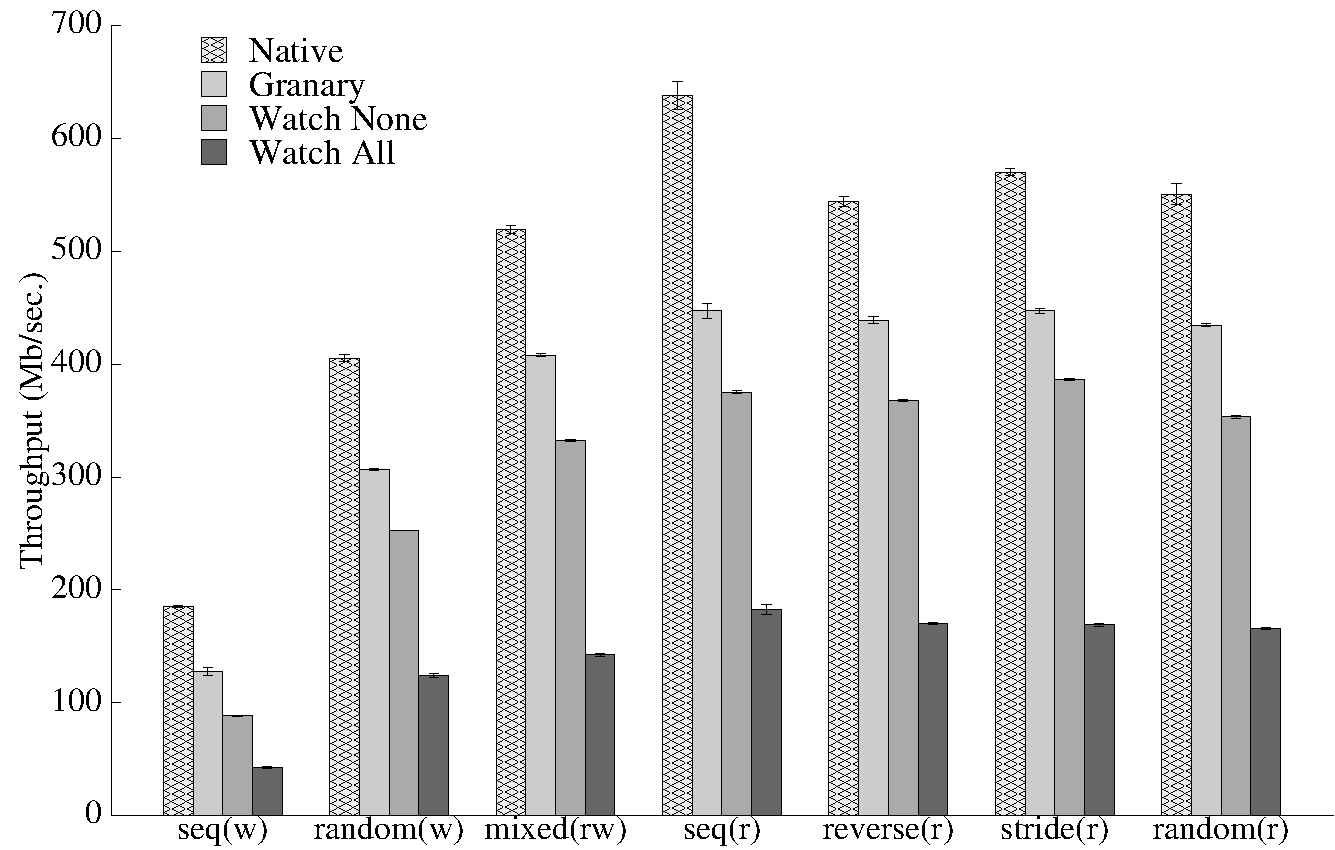
\includegraphics[width=4.5in]{thesis_code_driven.pdf}
\end{center}
\caption[Performance impact of code centric instrumentation.]{\label{fig:watchpoint_performance_code_driven}Throughput in MB/sec of common file system operations for code-centric instrumentation. Direct IO is enabled to bypass the effect of the OS buffer cache on read requests. It compares the overhead of the watchpoint framework with the performance overhead of Granary and with native system.}
\end{figure}

\subsection{Iozone filesystem benchmark}
We used the \emph{iozone}~\cite{citeulike:919086} file system benchmark to measure the overhead of behavioral watchpoints on the throughput of common file system operations. In our experimental setup, we used the \texttt{ext3} file system module that was mounted on a RAMDisk of size 1GB. We enabled direct IO to avoid the effect of buffer cache on file system. The \emph{iozone}, in throughput mode, created two processes (reader, writer) that perform the file I/O operations on a file of size 480Mb with a record size of 4Kb. The watchpoint framework wraps the two most commonly used memory allocators in \texttt{ext3} and \texttt{jbd}: \texttt{\_\_kmalloc} and \texttt{kmem\_cache\_alloc}, to add watchpoints on the allocated objects. We evaluated both the code-centric \& data-centric approaches using \emph{iozone} and compared their performance.


%----

%We evaluated both code-centric and data-centric approach using \emph{iozone} and compared their performance in terms of the number of active watchpoints. 
%In data-centric instrumentation approach the behavioral watchpoint does not uses wrappers for attaching and detaching Granary at the interface. The framework attaches on traps raised by dereferencing of watched addresses and it detaches at the end of basic block or when the function returns. In this case we wrap the allocators by hot-patching kernel text and add watchpoints only when the allocation happens by the module code. 

\begin{table*}
\begin{center}
\vspace{1em}
\begin{tabular}{|l|r|r|}
  \hline
  \multicolumn{3}{|c|}{Watchpoint statistics for the code-centric instrumentations}  \\ \hline
  \hline
  & Watch None & Watch All \\
  \hline
  Number of basic blocks & 2249 & 5495\\
  \hline
  Number of basic blocks with watched memory operations & 0 & 1208\\
  \hline
  Number of executed basic blocks & 238782485 &  825836778 \\
  \hline
  Number of dynamic memory operations & 568643857 & 1693113417 \\
  \hline
  Number of watched memory operations & 0 &199495293 \\
  \hline
  Number of kernel hardware traps & 0 & 12630779 \\
  \hline
\end{tabular}
\caption[Watchpoint statistics for code centric instrumentation. The watchpoints are added on all module allocated objects.]{\label{table:code-centric-watchpoint_stats} The statistics of the watchpoint framework for code-driven instrumentation when module allocated objects are watched. It also shows the effect of watched objects leaked to the kernel. The increase in the number of hardware traps causes an increase in the number of basic blocks and the number of executed basic blocks.}
\end{center}
\end{table*}

\paragraph{Code-centric instrumentation:}
The code-centric approach comprehensively instruments the module code and dynamically adds watchpoint instrumentation at every memory reference. This baseline watchpoint instrumentation causes overhead even when there are no added watchpoints. In the code-centric approach the module always runs under the control of Granary and executes code from the code-cache. It uses the kernel and module function wrappers for fast attaching and detaching at the interface. %This causes an extra overhead on any interactions between the kernel and the modules.

In the code-centric instrumentation, we first evaluated the overhead of watchpoint instrumentation and the cost of using Granary as the underlying DBT system. This is important to understand the baseline cost of using the watchpoint framework. 

\Figref{watchpoint_performance_code_driven} represents the overhead of code-centric instrumentation on the throughput of file I/O operations. The overhead of the watchpoint framework increases to {\texttildelow}70\% when all objects allocated by the module are watched. This is because many of these watched objects are shared and leak to the kernel. When these objects are dereferenced in the kernel, they cause hardware traps because Granary detaches itself at the kernel interface and the watchpoint instrumentation is no longer added to the memory references. These hardware traps are costly and reattach the watchpoint framework which then instruments the kernel code transitively.


\begin{table*}
\begin{center}
%\caption{Performance of macrobenchmark}
\begin{tabular}{ |l||r|r|r| }
\hline
\multicolumn{4}{ |c| }{Access pattern of module allocated objects} \\ \hline
\hline
Memory Allocator & Size & Module Accesses Count  & Kernel Accesses Count\\ \hline
\multirow{5}{*}{$\_\_kmalloc$} & 8 & 1233865 & 0 \\ \cline{2-4}
 & 50 & 720 & 288\\ \cline{2-4}
 & 51 & 648 & 240\\ \cline{2-4}
 & 59 & 792 & 528\\ \cline{2-4}
 & 4096 & 23452 & 0 \\ \hline
 \hline
 \multirow{7}{*}{$kmem\_cache\_alloc$} & 16 & 31533 & 0 \\ \cline{2-4}
 & 24 & 25019188 & 0\\ \cline{2-4}
 & 32 & 2348 & 0\\ \cline{2-4}
 & 64 & 2469028 & 3099\\ \cline{2-4}
 & 112 & 21404553 & 0 \\ \cline{2-4}
 & 192 & 19902520 & 4916028 \\ \cline{2-4}
 & 768 & 57760206 & 37373718 \\ \cline{2-4}
 & 1024 & 34865132 & 7940485 \\ \cline{2-4}
 & 8196 & 299 & 821648 \\ \hline
 \hline
 \multirow{1}{*}{$\_get\_free\_page$} & 4096 & 820273 & 2973 \\ \hline
\end{tabular}
\caption[Memory access pattern of module allocated objects.]{\label{table:access_pattern_shared_objects}The memory accesses patten of the module allocated objects. It represents the number of times an object is getting accessed by the module and the kernel code. The objects are classified based on its size and the memory allocator used for allocation. %The post analysis  shows that file system \texttt{inode} objects with memory size 768 are most accessed object by the kernel. A watchpoint on \texttt{inode} object will generate maximum number of hardware traps.
}
\end{center}
\end{table*}

\begin{table*}
\begin{center}
\vspace{1em}
\begin{tabular}{|l|r|r|}
  \hline
  \multicolumn{3}{|c|}{Watchpoint statistics for the code-centric instrumentations}  \\ \hline
  \hline
  & Watch none \texttt{inode} & Watch All \\
  \hline
  Number of basic blocks & 2874 & 5495\\
  \hline
  Number of basic blocks with watched memory operations & 732 & 1208\\
  \hline
  Number of executed basic blocks & 266083908 &  825836778 \\
  \hline
  Number of dynamic memory operations & 594195510 & 1693113417 \\
  \hline
  Number of watched memory operations & 92600064 &199495293 \\
  \hline
  Number of kernel hardware traps & 5285701 & 12630779 \\
  \hline
\end{tabular}
\caption[Watchpoint statistics for code centric instrumentation. The watchpoints are added on all the module allocated objects except file \texttt{inode}s.]{\label{table:code-centric-node-inode-watchpoint_stats} The watchpoint statistics of the framework for code-driven instrumentation when all objects allocated by the modules (except \texttt{inode}s) are watched.}
\end{center}
\end{table*}

Table~\ref{table:code-centric-watchpoint_stats} represents the number of hardware traps encountered and number of executed basic blocks for the code centric instrumentation. The additional increase in the number of basic blocks ({\texttildelow}2.5{\footnotesize$\times$}) and the number of executed basic blocks ({\texttildelow}3.5{\footnotesize$\times$}) comes due to the kernel code instrumentation on hardware traps. It also shows that the one out of every sixteen watched memory operations causes hardware traps.

For understanding the source of these hardware traps, we developed a tool using the watchpoint framework which tracks the accesses of module allocated objects. We typed these objects based on their size and the memory allocator used for its allocation. Table~\ref{table:access_pattern_shared_objects} shows the access pattern of the module allocated objects. The post processing analysis shows that file system \texttt{inode} objects with its size ``768'' gets accessed by the kernel maximum number of times and adding watchpoint on \texttt{inode} objects cause maximum number of hardware traps.

We verified this by removing watchpoints from all \texttt{inode} objects and running \emph{iozone} in throughput mode. \Figref{watchpoint_performance_code_driven_none_inode} shows that the overhead for \emph{Watch All} decreases by {\texttildelow}50\% and is close to the overhead of baseline instrumentation i.e, \emph{Watch None}. The small differences in the overhead of \emph{Watch All} and \emph{Watch None} are because there were still some shared objects which was getting watched and causing hardware traps. Table~\ref{table:code-centric-node-inode-watchpoint_stats} shows the details about such objects.


\begin{figure}[t]
\begin{center}
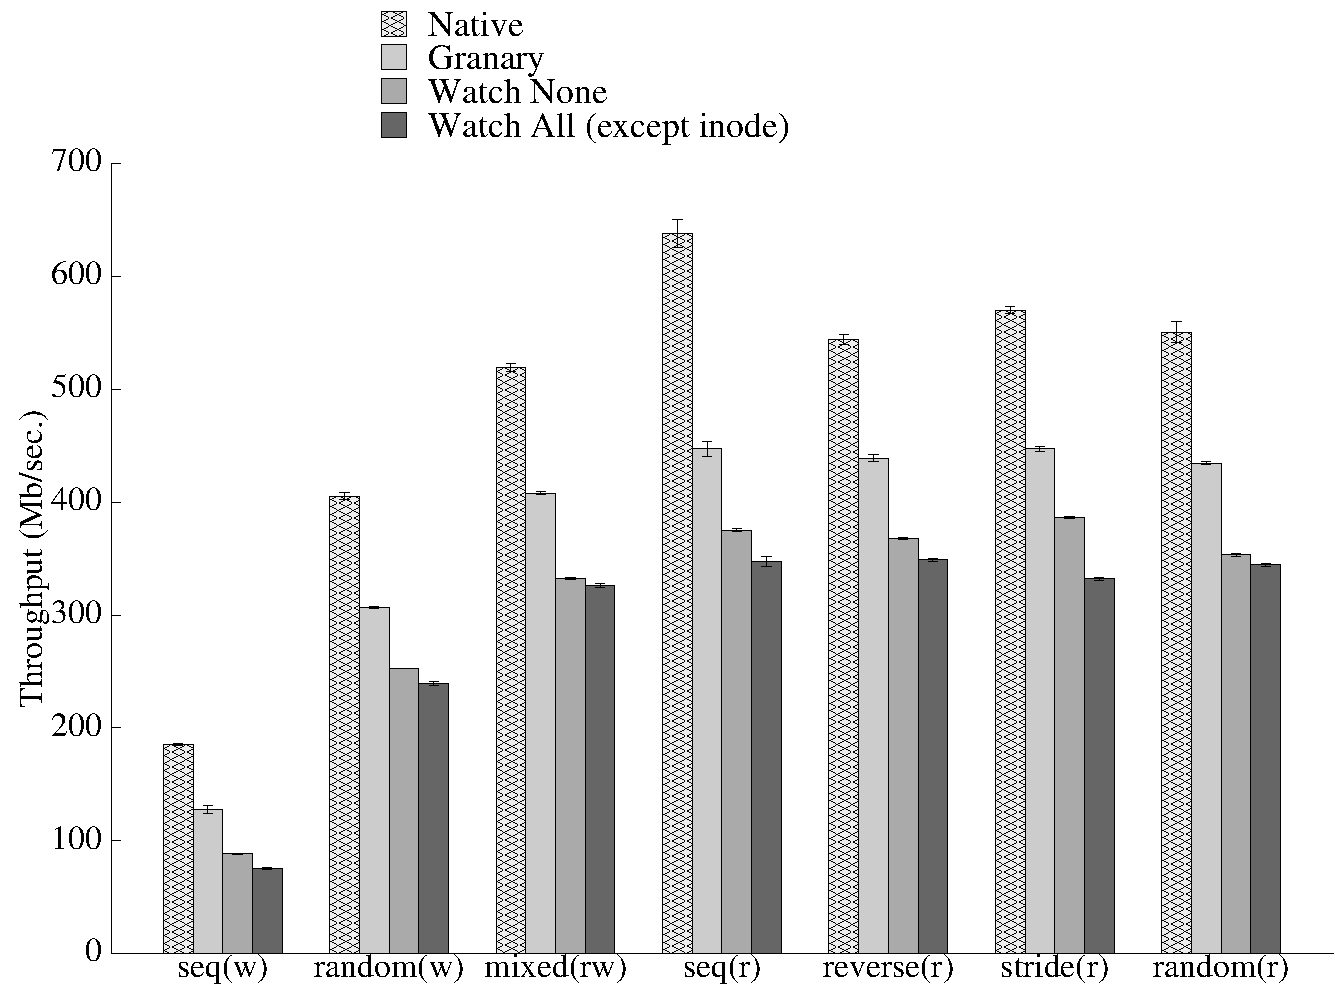
\includegraphics[width=4.5in]{thesis_code_none_inode.pdf}
\end{center}
\caption[Performance impact of code centric instrumentation. The watchpoints are added on all module allocated objects except file \texttt{inode}s.]{\label{fig:watchpoint_performance_code_driven_none_inode}Throughput in MB/sec of common file system operations for code-centric instrumentation when \texttt{inode} objects are not getting watched. The overhead of \emph{Watch All} decrease because of the less number of hardware traps and executed basic blocks.}
\end{figure}


The evaluation of code-centric instrumentation shows that the hardware traps on the kernel code are the major source of overhead in implementing behavioral watchpoints. These hardware traps can be removed by providing full kernel support to the code-centric instrumentation. Granary, being the underlying DBT-system, currently does not provide support for whole kernel instrumentation. 

%To understand the source of these hardware traps, we developed a tool using the watchpoint framework 


%We also studied the source of these hardware traps 


%The evaluation shows that a major contribution in the overhead of code-centric instrumentation comes due to Granary and its wrapping mechanism.

 %\Figref{watchpoint_performance_code_driven} shows the drop in throughput of filesystem operations when using the watchpoints instrumentation. As mentioned earlier \emph{watchpoint\_null} represents the overhead of baseline watchpoints instrumentation with no added watchpoints, and \emph{everything\_watched} shows the overhead where module-allocated objects are watched. We used code-centric instrumentation approach for the evaluation.

%In the previous section, we discussed that due to the limitations of Granary to instrument only the module code, our implementation of code-centric instrumentation is limited. We use code-centric instrumentation for executing the module code and data-centric instrumentation for the kernel code if the watchpoint leaks to the kernel. We also use three different policy for the code-centric instrumentation: transitive instrumentation policy, function-only instrumentation policy and basic-block instrumentation policy. The detail about these policies are discussed in section. Before evaluating the complete data-centric approach, we evaluated the compared the effect of three policies on code-centric instrumentation.



%\Figref{watchpoint_performance_code_driven} shows the overhead on the throughput of different filesystem operations. We also collected the watchpoint statistics for the the three policies. Table~\ref{table:data-centric-table} shows the number of hardware-exception encountered and the ration of executed basic block containing watched and unwatched addresses.

\begin{figure*}[t]
\begin{center}
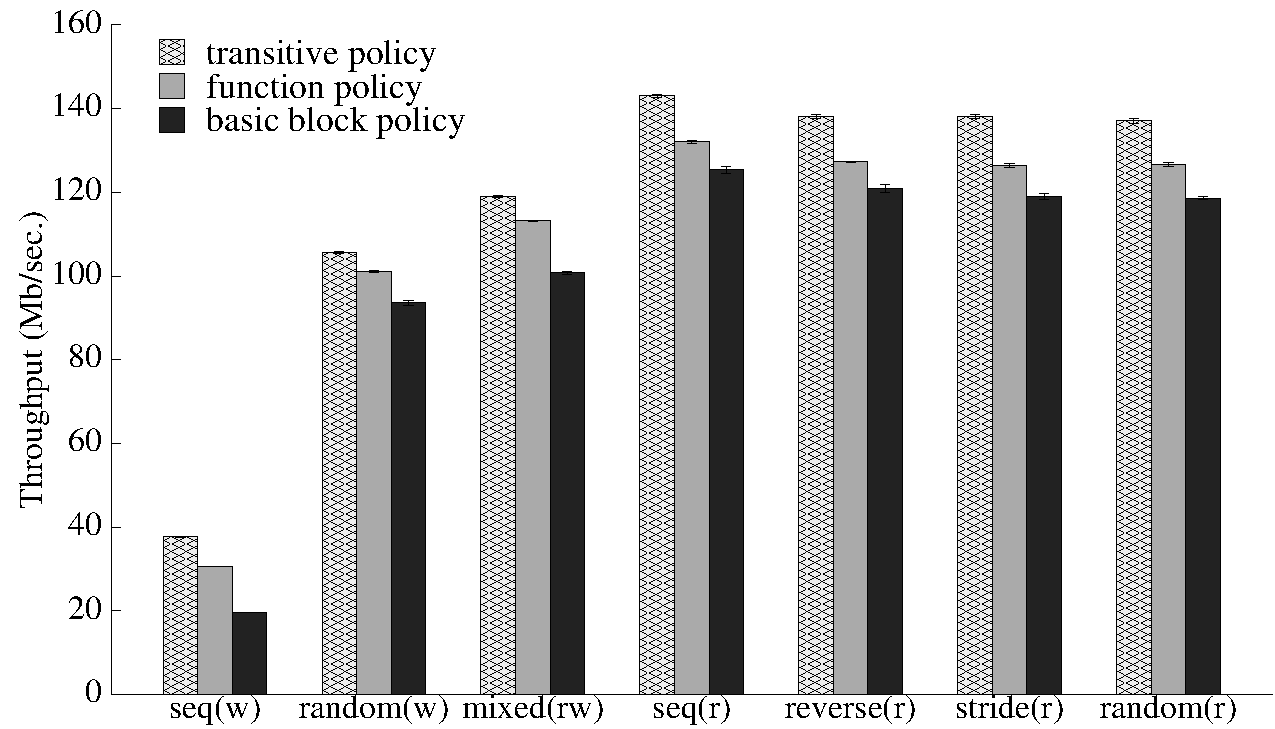
\includegraphics[width=4.5in]{thesis_data_driven.pdf}
\end{center}
\caption[Performance impact of data centric instrumentation.]{\label{fig:watchpoint_performance_data_driven}Throughput in MB/sec of common file system operations for data-centric instrumentation. It shows the overhead of three data-centric policies: transitive policy, function only, and basic block only policy.}
%for the watched address is shown.}
\end{figure*}


\paragraph{Data-centric instrumentation:}
We implemented data-centric instrumentation with three detach policies: i) transitive policy, ii) function-only policy and iii) basic block policy. Section~\ref{sec:data-centric} discusses each of the three policies in detail. %The data-centric instrumentation adds watchpoints on newly allocated objects through hot-patching and wrapping the kernel memory allocators. 


\begin{table*}
\begin{center}
\vspace{1em}
\begin{tabular}{|l|r|r|r|}
  \hline
  \multicolumn{4}{|c|}{Watchpoint statistics for data-centric instrumentation (with different detach policies)}  \\ \hline
  \hline
  & transitive & function & block \\
  \hline
  Number of basic blocks & 5755 & 3335 & 1144 \\
  \hline
  Number of basic blocks with watched memory operations & 1479 & 1218 & 1141\\
  \hline
  Number of executed basic blocks &  833167407  & 108965164 & 37378155\\
  \hline
  Number of dynamic memory operations & 1702295819 & 565666812 & 251985370\\
  \hline
  Number of watched memory operators & 336149753 & 234340514 & 206334774\\
  \hline
  Number of kernel hardware traps & 13403663 & 42259345 & 97518601\\
  \hline
  Number of module hardware traps & 112172 & 23496407 & 42902684\\
  \hline
\end{tabular}
\caption[Watchpoint statistics for data centric instrumentation.]{\label{table:data-centric-table} The statistics of the watchpoint framework for data-centric instrumentation when all the objects allocated by the modules are watched. It compares the three detach policies used by the data-centric approach.}
\end{center}
\end{table*}

We evaluated the overhead of data-centric instrumentation with \emph{iozone}, using the same experimental setup as with the code-centric instrumentations. We disabled the kernel and the module wrappers since they allow Granary to take complete control over the module code and prohibit the module code from running native. In data-centric instrumentation, the module code gets executed natively when there are no added watchpoints. 

Before comparing the code-centric and data-centric approaches, we first evaluated the three detach policies of data-centric instrumentation. \Figref{watchpoint_performance_data_driven} shows the overhead of each policy on the throughput of file I/O operations. The transitive policy instruments code aggressively and performs better than the function only and basic block detach policies. Table~\ref{table:data-centric-table} shows the number of executed basic blocks and the number of hardware traps encountered when each of the three detach policies are used. The transitive policy encounters the minimum number of hardware traps and executes the largest number of basic blocks. %The transitive policy also has large number of basic block with watched memory operations and this is because it adds more number of watchpoints on the newly allocated objects.

% executes the module code natively when no watchpoints get added and does not cause any runtime overhead in the system. It also uses three policies to reduce the cost of handling hardware traps. We first evaluated the three policies of data-centric instrumentation and compared their performance overhead along with the number of basic block executed and the hardware traps encountered by each of them. \Figref{watchpoint_performance_data_driven} shows the overhead of each policies on the throughput of file I/O operations for \texttt{ext3} module. The transitive policy has slight advantage over the function only and basic block policy because of the decrease in the number of hardware traps it needs to handle. There is also an increase in the number of basic block executed and this adds to the overhead of the transitive policy. Table~\ref{table:data-centric-table} shows how the number of executed basic blocks and the number of hardware traps encountered varies across the three policies. It also shows that the number of hardware traps encountered in module code is always less than the hardware traps at the kernel code. It represents that a majority of watched objects are shared and leaks to the kernel. These hardware traps also causes a significant overhead in the code-centric instrumentation and our approach of code-centric is more biased towards the data-centric.


\begin{figure}[t]
\begin{center}
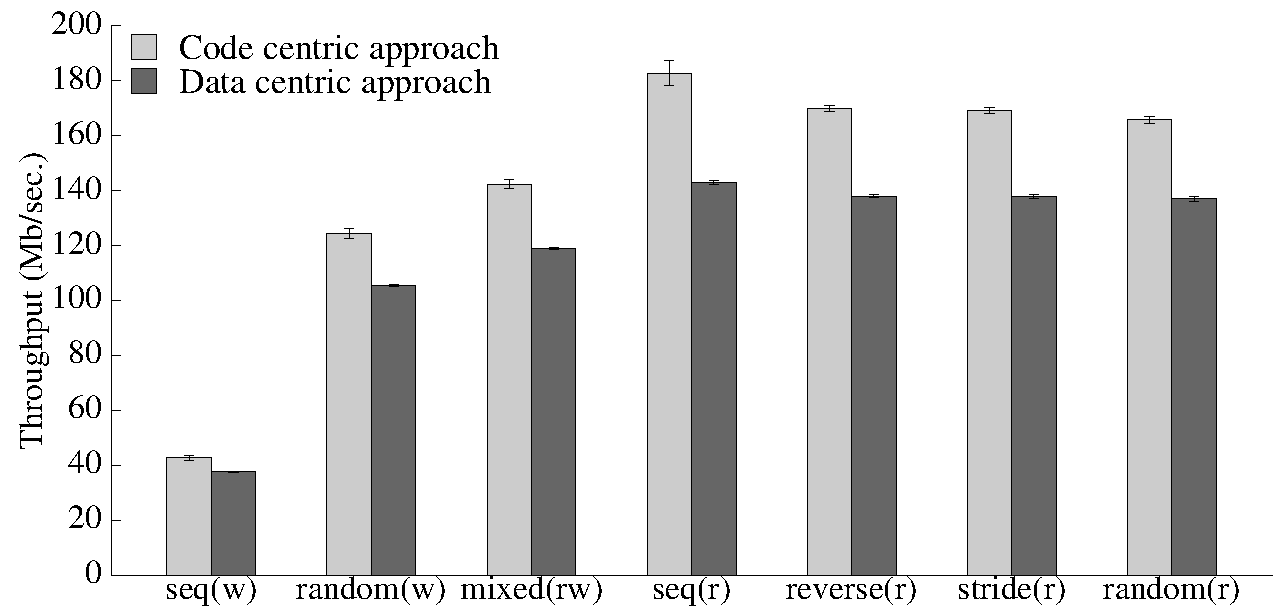
\includegraphics[width=6.0in]{thesis_data_code.pdf}
\end{center}
\caption[Performance impact of Data centric Vs Code centric instrumentation.]{\label{fig:watchpoint_performance}Throughput in MB/sec of common file system operations for the code-centric and data-centric approaches. The watchpoints are added on all objects allocated by the module.}
%for the watched address is shown.}
\end{figure}

%of the two reasons: i) the data-centric instrumentation handles more hardware traps which is costly, and ii) the number of watchpoints added in transitive detach policy is more than the code-centric instrumentations.

%In spite of increase in the number of hardware traps in the data-centric approach, it is performing better than the code-centric approach. This is because of the increase in the number of executed basic blocks. Also the code-centric approach suffers significantly due to the large number of hardware traps in the kernel code. The evaluation of three policies of data-centric approach also shows that the increase in the overhead due to hardware traps is getting compensated with the less number of basic block being executed. Table~\ref{table:data-centric-table} shows that the number of hardware traps encountered in transitive policy is 5x less than the basic block policy but it is executing 10x more basic block and thus not getting much advantages in terms of performance. The code centric approach is also using the kernel and the module wrappers which has an additional cost.

\begin{figure}[!h]
\begin{center}
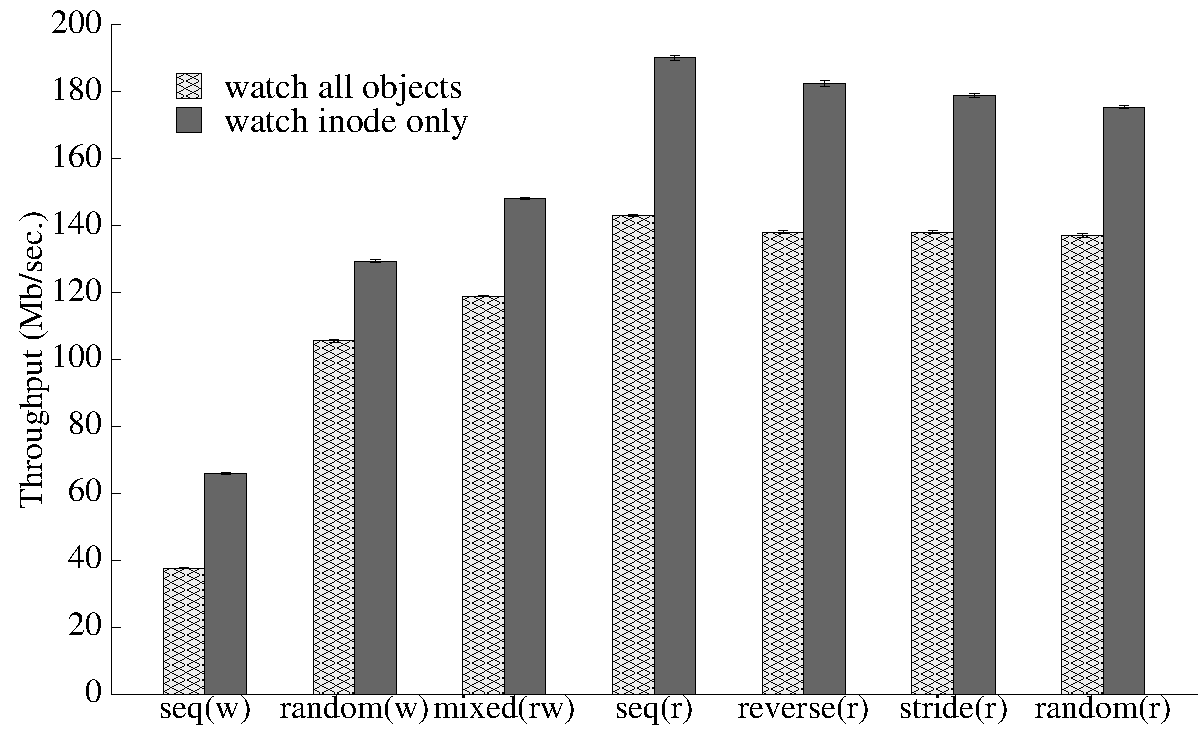
\includegraphics[width=6.0in]{thesis_watch_inode.pdf}
\end{center}
%\end{figure}

%\begin{figure}
\begin{center}
\vspace{1em}
\begin{tabular}{|l|r|r|}
  \hline
  \multicolumn{3}{|c|}{Watchpoint statistics for selective instrumentation in data centric instrumentation }  \\ \hline
  \hline
  & Watch \texttt{inode}s & Watch all \\
  \hline
  Number of basic blocks & 4217 & 5755\\
 % \hline
  Number of basic blocks with watched memory operations & 562 & 1479 \\
  \hline
  Number of executed basic blocks &  735367411 &  833167407 \\
  \hline
  Number of dynamic memory operations & 1519057148 & 1702295819 \\
  \hline
  Number of watched memory operators & 87433900 & 336149753 \\
  \hline
  Number of kernel hardware traps & 5522314 &  13403663 \\
  \hline
  Number of module hardware traps & 11234 & 112172 \\
  \hline
\end{tabular}
%\caption{\label{fig:watchpoint_inode_compare} Throughput in MB/sec of common file system operations and the watchpoint statistics when watchpoints are added selectively and only on \texttt{inode} objects.}
\caption[Performance impact of selective instrumentations for data-centric approach.]{\label{fig:watchpoint_inode}Throughput in MB/sec of common file system operations and the watchpoint statistics for data-centric instrumentation when watchpoints are added selectively and only for \texttt{inode} objects. The evaluation is done for transitive detach policy.}
%for the watched address is shown.}
\end{center}
\end{figure}


\Figref{watchpoint_performance} compares the overhead of code centric and data centric instrumentation. It shows that the code centric instrumentation performs better than the data centric instrumentation when all objects allocated by the module are watched. This is because the code centric instrumentation handles less hardware traps, which is costly and affects the performance of the system. Our evaluation compares the code centric instrumentation with the data centric instrumentation using transitive detach policy.


\begin{figure}[!h]
\begin{center}
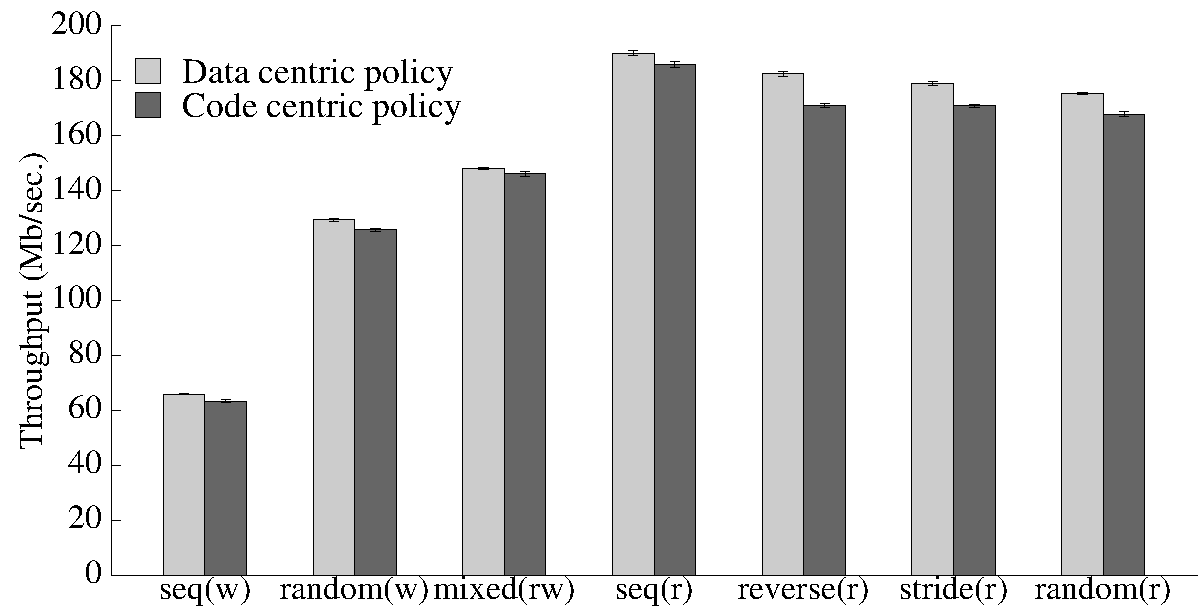
\includegraphics[width=6.0in]{thesis_watch_inode_compare.pdf}
\end{center}
%\caption{\label{fig:watchpoint_inode_compare}Throughput in MB/sec of common file system operations when watchpoints are added selectively and only for \texttt{inode} objects. The evaluation is done with transitive instrumentation policy.}
%for the watched address is shown.}
%\end{figure}  

%\begin{table*}
\begin{center}
\vspace{1em}
\begin{tabular}{|l|r|r|}
  \hline
  \multicolumn{3}{|c|}{Watchpoint statistics for selective instrumentation (watch \texttt{inode} objects)}  \\ \hline
  \hline
  & Code centric & Data centric \\
  \hline
  Number of basic blocks & 5405 & 4217 \\
 % \hline
  %Number of basic blocks with watched memory operations & 563 & 563 \\
  \hline
  Number of executed basic blocks &  814496751  & 735367411 \\
  \hline
  Number of dynamic memory operations & 1684738365 & 1519057148\\
  \hline
  Number of watched memory operators & 91699675 & 87433900 \\
  \hline
  Number of kernel hardware traps & 5446745 & 5522314 \\
  \hline
  Number of module hardware traps & 0 & 11234 \\
  \hline
\end{tabular}
\caption[Performance impact of selective instrumentations. The watchpoints are added on all file \texttt{inode} objects.]{\label{fig:watchpoint_inode_compare} Throughput in MB/sec of common file system operations and the watchpoint statistics when watchpoints are added selectively and only on \texttt{inode} objects.}
\end{center}
%\end{table*}
\end{figure}



\begin{figure}[!h]
\begin{center}
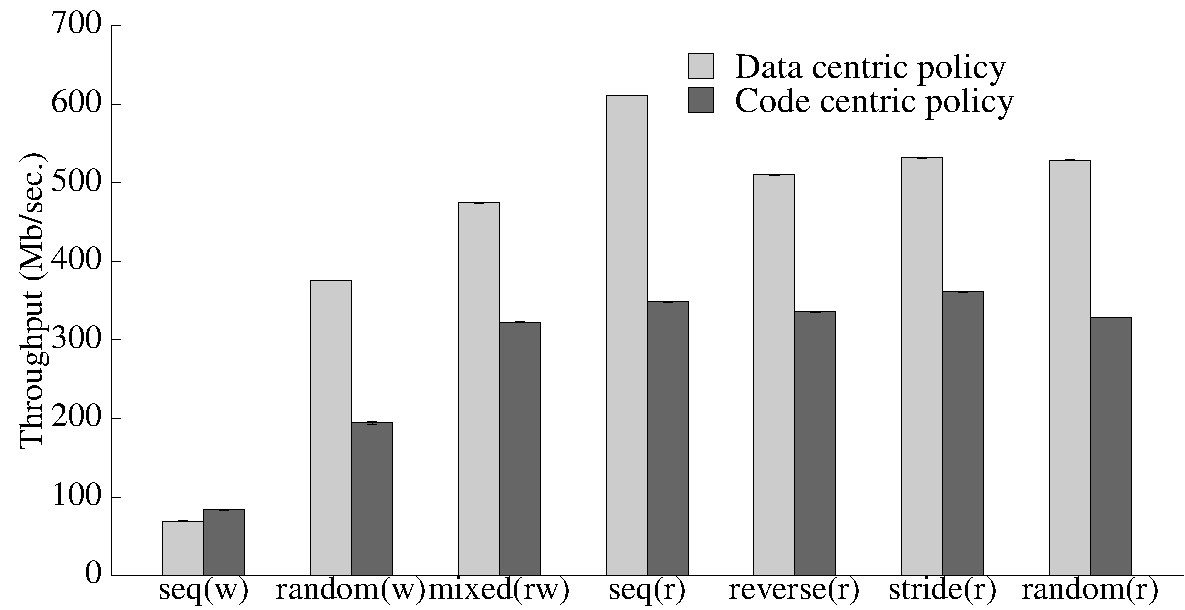
\includegraphics[width=6.0in]{thesis_selective_watch_no_inode.pdf}
\end{center}
\vspace{1em}
\begin{center}
\begin{tabular}{|l|r|r|}
  \hline
  \multicolumn{3}{|c|}{Watchpoint statistics for selective instrumentation (no hardware traps on kernel code)}  \\ \hline
  \hline
  & Code centric & Data centric \\
  \hline
  Number of basic blocks & 2259 & 1171 \\
  \hline
  Number of basic blocks with watched memory operations & 179 & 189 \\
  \hline
  Number of executed basic blocks &  238740476  & 105345884 \\
  \hline
  Number of dynamic memory operations & 568556578 & 221904835\\
  \hline
  Number of watched memory operators & 45649624 & 45637811\\
  \hline
  Number of module hardware traps & 0 & 10244480 \\
  \hline
\end{tabular}
\caption[Performance impact of selective instrumentations. The watchpoints are added on objects that are not getting accessed by the kernel code]{\label{fig:watchpoint_none_inode_compare} Throughput in MB/sec of common file I/O operations and the statistics of the watchpoint framework when watchpoints are added to the objects selectively which are not getting accessed by the kernel. This removes the effect of hardware traps from the code-centric instrumentations.}
\end{center}
%\end{table*}
\end{figure}
%on the throughput of file operations when only inode gets watched. In this case we used transitive policy for the evaluation.  

\paragraph{Selective instrumentation:}
The data centric approach enables selective instrumentation by adding watchpoints on selected objects. We first evaluated the performance of selective instrumentation by adding watchpoints only on file \texttt{inode} objects. \Figref{watchpoint_inode} shows the overhead of selective instrumentation and compares it with the overhead of data-centric instrumentation when all the module allocated objects are watched. Selective instrumentation performs better since it adds less watchpoints thus encountering fewer hardware traps, and executing fewer instrumented basic blocks.

We also compared the performance of selective instrumentation when using code-centric and data-centric approaches. \Figref{watchpoint_inode_compare} compares the overhead of selective instrumentation for both the approaches. It shows that selective instrumentation using data centric instrumentation has less overhead than with code centric instrumentation. This is because fewer basic blocks gets executed with data-centric instrumentation. The number of hardware traps encountered in both the approaches are also approximately same, causing similar overhead. 


The evaluation of code-centric approach shows that a major source of overhead in code-centric instrumentation comes due to adding watchpoints on file \texttt{inode} objects. These objects gets accessed mostly by the kernel code causing hardware traps. We removed the effect of these hardware traps from code-centric instrumentation by adding watchpoints selectively on the objects accessed only by the modules. We took the help of table~\ref{table:access_pattern_shared_objects} for adding watchpoints on the objects selectively.

 \Figref{watchpoint_none_inode_compare} represents the overhead of selective instrumentations for data-centric approach and compares it with the code-centric instrumentation. It shows that the selective instrumentation reduces the overhead of using the watchpoint framework to {\texttildelow}5\% where as the baseline instrumentation for code-centric approach causes an overhead of {\texttildelow}40\%. This is because the selective instrumentation executes less number of basic blocks ({\texttildelow}2.3{\footnotesize$\times$}). The evaluation also shows that the performance of sequential write operation in case of data-centric approach is less than the code-centric. We analyzed the behavioral of write operations and found that {\texttildelow}50\% of the total hardware traps was only happening during sequential write operations. This could be a reason of sequential write not performing better.    

 The evaluation of both, the code-centric and data-centric approaches for implementing behavioral watchpoints, shows an interesting trade-off between the amount of instrumented code executed from the code-cache and how much of that code actually needs to be instrumented. The code-centric approach always suffers from the overhead of baseline instrumentation since it always executes instrumented basic block from code cache. The data-centric instrumentation overcome this by adding instrumentation on-demand. However, it suffers from the high cost of the hardware traps which triggers the instrumentation. The number of executed basic blocks also increases with the hardware traps which causes additional overhead.

 We also saw that the number of hardware traps depend on the type of the watched objects. Adding watchpoints on frequently accessed shared objects such as file \texttt{inode}s, causes a large number of traps affecting the performance of the watchpoint framework where as watching relatively less accessed objects such as \texttt{ext3\_block\_alloc\_info} causes less traps improving the performance of the data-centric instrumentation.

 The advantages and disadvantaged of both the approaches opens up the space to further explore the possibility of switching between the two approaches at runtime. This will reduce both the overhead of baseline instrumentation and the cost of hardware traps, thus improving the performance of the system. The evaluation of code-centric instrumentation also shows its need to provide the whole kernel instrumentation support. We plan to take this as an immediate future work.

 %The evaluation of the watchpoint framework using \emph{iozone} shows the


 %It shows that the selective instrumentation using data-centric approach reduces the overhead of using the watchpoint framework 


 %for both the code-centric and data-centric approaches.



 %by adding watchpoints on such objects. The data centric instrumentation in such case performs much better than the code centric approach and the performance of data centric instrumentation is close to that of the native system. 


%and added watchpoints selectively on objects which does not get accessed by the kernel.


%, we saw that a major source of overhead in code centric approach is the number of hardware traps. Much of these hardware traps occur due to adding watchpoints on \texttt{inode} objects and the code centric instrumentation was performing worse when it was getting watched. To remove the effect of hardware traps in selective instrumentation, we took the help of table~\ref{table:access_pattern_shared_objects} and added watchpoints selectively on objects which does not get accessed by the kernel. \Figref{watchpoint_none_inode_compare} compares the overhead of selective instrumentations by adding watchpoints on such objects. The data centric instrumentation in such case performs much better than the code centric approach and the performance of data centric instrumentation is close to that of the native system. 

%the number of instrumented basic block executed in case of data-centric approach is less than the code-centric approach. 
%However, it also shows that there are more hardware traps encountered with data-centric approach.

%The watchpoint gets added to the objects selectively. We evaluated the performance of selective instrumentation by adding watchpoints only to the \texttt{inode}s. \Figref{watchpoint_inode} compares the overhead on the throughput of file operations when only inode gets watched. In this case we used transitive policy for the evaluation.   
% the overhead of code-centric and data-centric approach 

%using complete data-centric approach.



%from providing the complete data-centric approach by wrapping all the function pointers at the interface for faster attach and detach.

%and we also used the same experimental setup for running the benchmark. We also disabled the wrappers for fast attach and detach since it prohibits the framework from providing the complete data-centric approach by wrapping all the function pointers at the interface for faster attach and detach.


%\subsection{Filebench}
%We evaluated the real workload using Filebench file system benchmark.

\subsection{Macrobenchmark}
We further evaluated the overhead of the behavioral watchpoint framework using a file system macrobenchmark consisting common system utilities. We used the same experimental setup and mounted the \texttt{ext3} module on a RAMDisk of size 1GB. The macrobenchmark operated on the Linux source tree (\texttt{linux-3.2.50}). Table~\ref{table:system_utils-benchmark} shows the overhead of behavioral watchpoints on the standard system utilities. For both the code-centric and data-centric approaches, the framework adds watchpoints selectively on all \texttt{inode} objects allocated from the look-aside buffer. The evaluation shows data-centric instrumentation is performing better than code-centric instrumentation when used for watching objects selectively all the \texttt{inode} objects.


\begin{table*}
\begin{center}
\vspace{1em}
\begin{tabular}{|l|r|r|r|}
  \hline
   & Native execution & Data centric approach & Code centric approach \\
  \hline
  cp & 6.64 & 10.82 & 11.61\\
  \hline
  tar & 2.64 & 3.84 & 4.16\\
  \hline
  stat & 3.90 & 5.12 & 5.44\\
  \hline
  grep & 3.94 & 5.36 & 5.54\\
  \hline
\end{tabular}
\caption[Performance impact of the watchpoint framework on macrobenchmark]{\label{table:system_utils-benchmark}The CPU (system \& user) time for the standard system utilities performing file system operations on a RAMDisk of size 1GB. The framework adds watchpoints selectively on all \texttt{inode} objects of the \texttt{ext3} module.}
\end{center}
\end{table*}


\begin{figure*}[t!]
\begin{multicols}{2}
\begin{center}
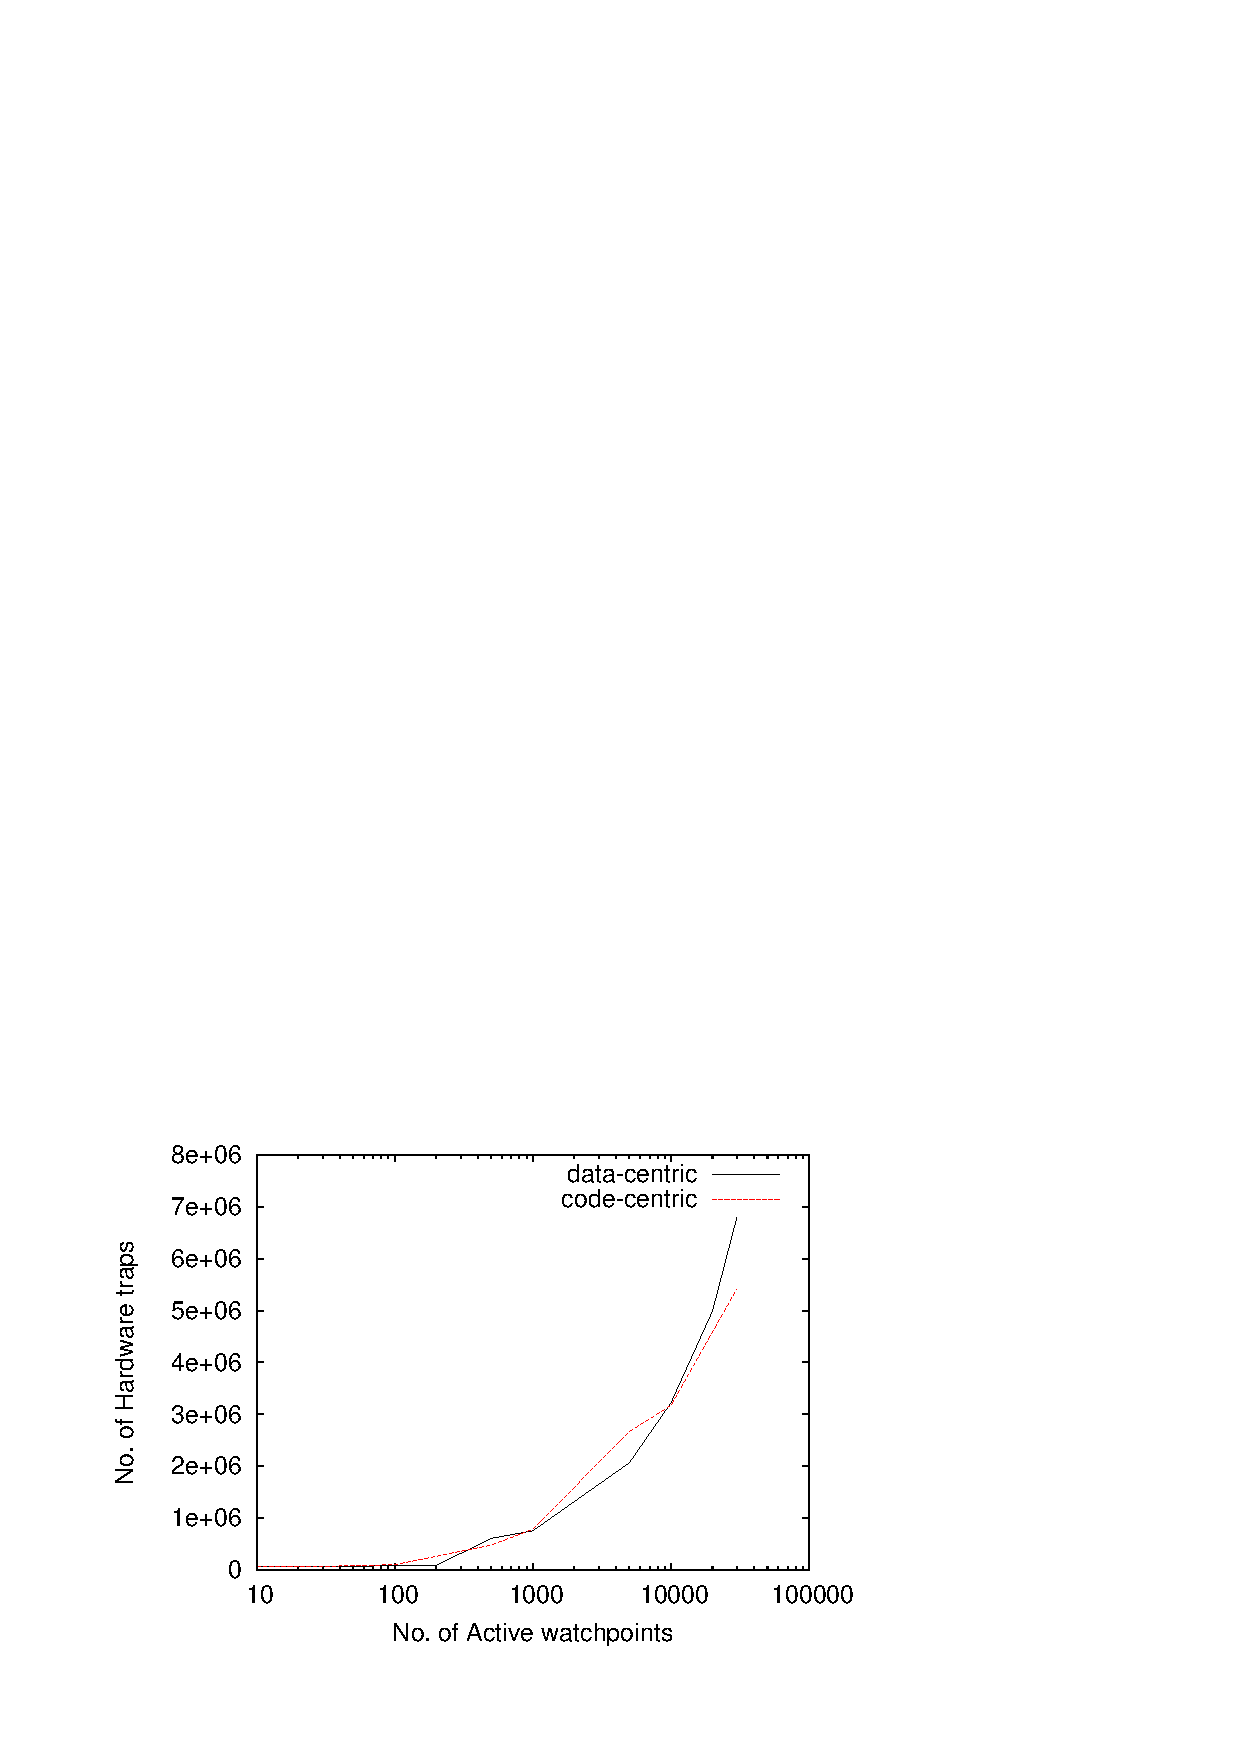
\includegraphics[width=3.5in]{hardware_traps.pdf}
\end{center}
\columnbreak
\begin{center}
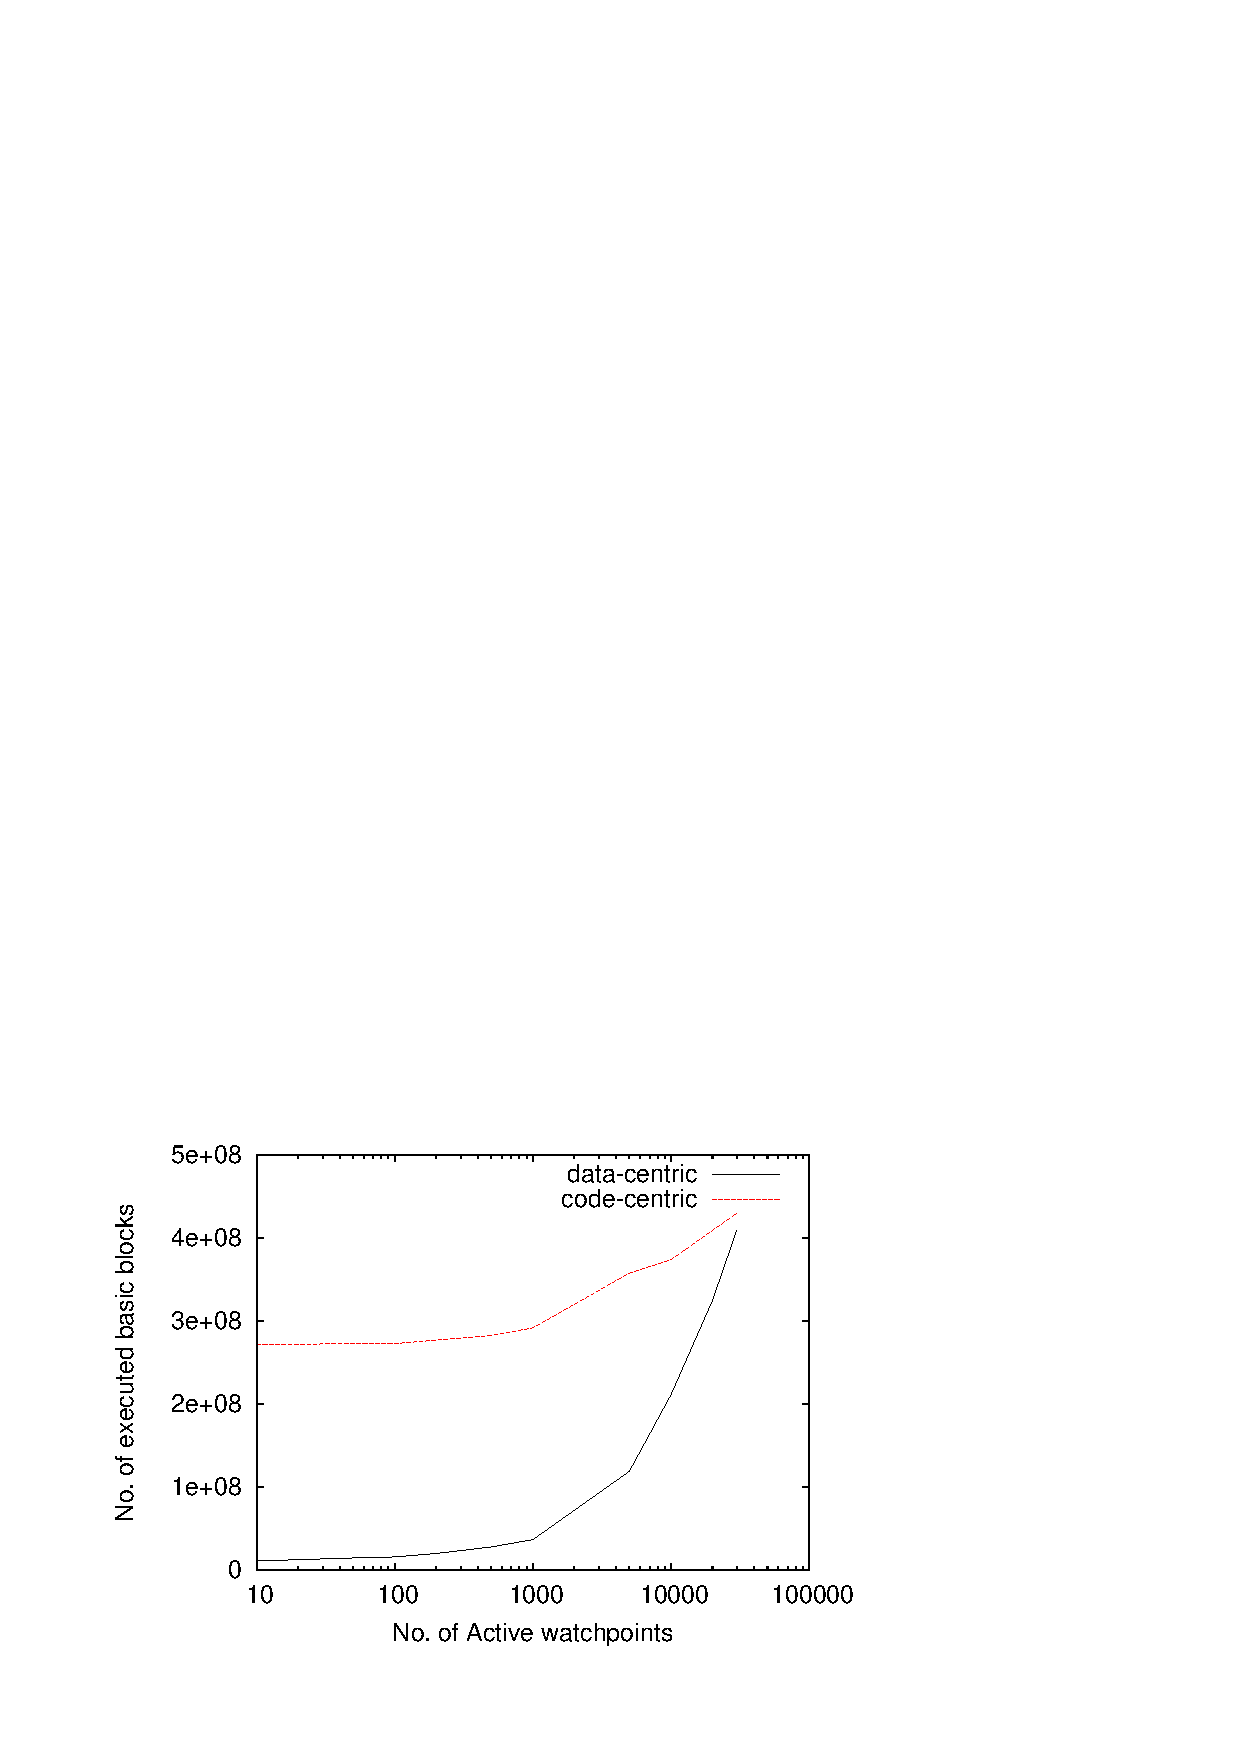
\includegraphics[width=3.5in]{executed_bb_data.pdf}
\end{center}
\end{multicols}
\caption[Cost profile of the watchpoint framework in terms of number of added watchpoints.]{\label{fig:traps_profile}The changes in the number of hardware traps and the number of executed basic blocks with the changes in number of added watchpoints.}
\end{figure*}

In both the code-centric and data centric approaches, the major factors which affects the performance are the number of basic block executed and the number of hardware traps encountered during the execution. We also used microbenchmark to study the changes in the number of hardware traps and the basic block executed with the change in the number of watchpoints. \Figref{traps_profile} shows that both the code centric instrumentation and data centric instrumentation encounters same number of hardware traps. This is because we add watchpoints selectively on all \texttt{inode} objects which gets accessed both by the module and the kernel code equally causing hardware traps. We also see fewer occurrences where the number of traps in case of data centric is less than the code centric instrumentation. One reason for this could be that the code centric instrumentation always detaches itself at the interface where as the data centric instrumentation, with transitive detach policy, does not always detaches itself at the interface.

\Figref{traps_profile} also shows that with fewer watchpoints the code centric instrumentation still executes many more basic blocks than the data centric approach. This causes increased overhead for code centric instrumentation even when fewer watchpoints are added. 




% and causes more overhead even when the 


% We also discussed previously that data centric instrumentation is useful when watchpoints are added on objects 

\begin{table*}
\begin{center}
\vspace{1em}
\begin{tabular}{|l|l|l|}
  \hline
   Workload & Setting & Data Size \\
  \hline
  Fileserver & nfiles=10K & 1.2GB \\
  \hline
  Webserver & nfiles=1K, & 14.76MB \\
  \hline
  Webproxy & nfiles=10K & 154MB \\
  \hline
  Varmail & nfiles=1K & 14.76MB \\
  \hline
\end{tabular}
\caption[Filebench server benchmark workload characteristics.]{\label{table:filebench-benchmark}Benchmark characteristics.}
\end{center}
\end{table*}


\begin{figure}[!h]
\begin{center}
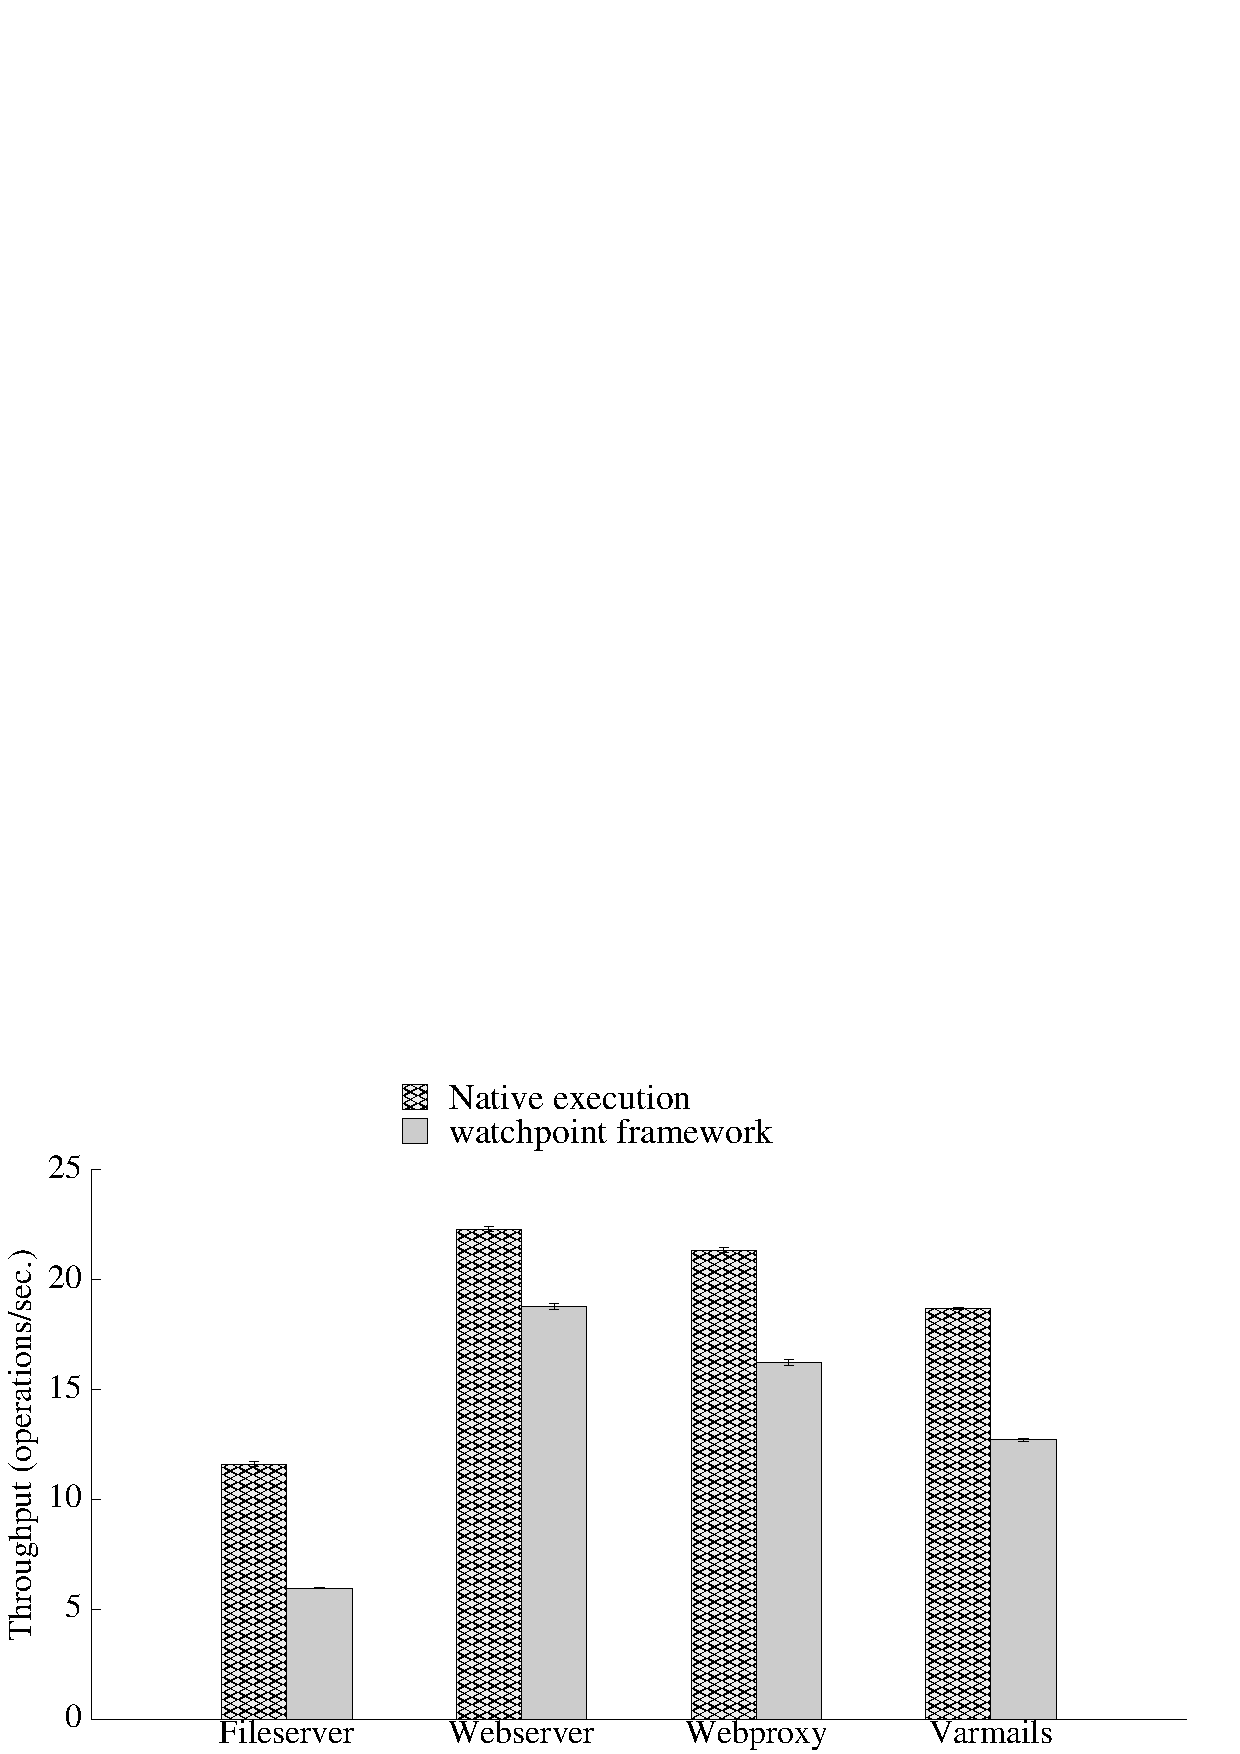
\includegraphics[width=6.0in]{filebench.pdf}
\end{center}
\caption[Performance impact of the watchpoint framework on Filebench server benchmark workloads.]{\label{fig:sever_performance}Throughput in file system operations/sec for the filebench workload personalities shown in Table~\ref{table:filebench-benchmark}.}
%for the watched address is shown.}
\end{figure}




\subsection{Server Benchmark}
We used the Linux port of Filebench version 1.4.9, with four of the standard server workload personalities, to evaluate the watchpoint framework. We used the same experimental setup as with the \emph{iozone} and enabled default settings to define the workload characteristics. The relevant characteristics for the workloads are shown in Table~\ref{table:filebench-benchmark}. With the default characteristics, the datasets easily fit in the RAMDisk used for evaluation. This does not limit the workload with the performance of I/O operations.

\Figref{sever_performance} shows the throughput of the different Filebench server workloads. For evaluation we used data-centric instrumentation with all file \texttt{inode} objects getting watched. The data centric instrumentation reduces the throughput for all the workload personalities by ~40\%. We also evaluated the code-centric instrumentation using Filebench and noticed similar drop in the throughput but we are not showing it here.

%Null Client reduces
%throughput by 3X for fileserver, and by 4.5X and 4.2X for webserver
%and webproxy, respectively. There is only a small additional
%reduction in throughput with Instruction Count. We can see that
%the drop in throughput is correlated with the number of threads
%used in the workload, with webserver and webproxy both using
%100 threads. The overhead for varmail, which syncs its data to disk
%frequently, is much lower, with only a 1.4X drop in throughput.

%We also evaluated the performance of behavioral watchpoints using real workloads. We mounted \texttt{ext3} file system module on a disk of size 20GB and used Filebench to simulate the real workloads. Table~\ref{table:filebench-benchmark} shows the characteristics of the workload we used for the evaluation.


%We used same experimental setup and mounted \texttt{ext3} module on RAMDisk of size 1GB. The macrobenchmark operated on the source tree of \texttt{linux-3.2.50} branch. We used the following five benchmarks to evaluate the performance overhead of the watchpoint framework: 

%\begin{enumerate}
%	\item \emph{MakeDir:} It reads the directories subtree of source program and constructs the identical target directories subtree. It uses \texttt{mkdir} utility for creating the directories recursively.
%	\item \emph{Copy:} It copies all the files from source files subtree to the target files subtree. We used \texttt{rsync} command to copy the files from the source directory to the target directory.
%	\item \emph{ScanDir:} It recursively goes to all the files in target directory and performs the stat operation on each file.
%	\item \emph{ReadAll:} It reads every byte of the every file in the target directory.
%	\item \emph{Compile:} It compiles and links all the files for the source program.
%\end{enumerate}


%Behavioral watchpoints uses non-canonical address to add watchpoints with the allocated objects. This provides the opportunity to implement data-centric instrumentation. Data-centric instrumentation is particularly important when watchpoints are unlikely to be triggered. We implemented three different policy for data-centric instrumentation: i) transitive policy, ii) function-only policy and iii) basic block policy. The details about it is provided in section. 

%Data-centric instrumentation also uses three different instrumentation policies and the details of which is provided in section.
%We used \emph{iozone} to evaluate the performance of data-centric instrumentation and we also used the same experimental setup for running the benchmark. We also disabled the wrappers for fast attach and detach since it prohibits the framework from providing the complete data-centric approach by wrapping all the function pointers at the interface for faster attach and detach.

%In this experiment, We studied the effect of hardware exceptions and watchpoint instrumentation overhead on the performance of filesystem throughput. We used the three data-centric policies for the evaluation and compared their performance in terms of the number of hardware exception encountered and the number of instrumented basic block executed. 

%Figure~\ref{fig:watchpoint_performance_data_driven} shows the throughput of common filesystem operations for data-centric instrumentation approach. Table~\ref{table:data-centric-table} shows the number of traps encountered along with the number of executed basic block and number of memory operations performed. The evaluation result shows the performance decrease with the number of traps but it gets compensated by executing less number of basic blocks and performing less number of memory operation which has an additional cost of watchpoint instrumentation.

% We also evaluated the number of hardware exception encountered and the number of basic block executed for each policies.



 %We also varies the number of watchpoints to see how the cost of data-centric instrumentation varies with the number of added watchpoints.


%These allocated objects when gets accessed causes hardware exceptions or traps. Behavioral watchpoint framework uses this to implement watchpoint instrumentation on trap. This approach allows selective instrumentation and can take advantage of low overhead when watchpoints are unlikely to be triggered. The trap-based instrumentation approach uses three different instrumentation policy: policy 1 includes the transitive instrumentation where the framework attaches itself on trap and instruments till it finds the indirect call or return and detaches itself. Policy 2 instruments the body of the function which encounters the trap and changes policy to go native on call and return. Policy 3 is the most conservative policy and tries to instruments minimum of the code. The instrumentation framework attaches itself on trap and detaches and goes to native execution on any control transfer, instrumenting only single basic block at a time. We evaluated all the three instrumentation policy by running the \emph{Iozone}~\cite{citeulike:919086} and studying the throughput of common file system operations. In trap-based instrumentation approach behavioral watchpoint is implemented on trap. We also used microbenchmark to evaluate the cost of taking trap and studied how the number of these traps increases over different policy and affects the performance.







%One of the important feature of data-driven instrumentation is the ability to watch objects selectively. The selective addition of watchpoints will have less instrumentation cost and also the number of hardware exception encountered will be less. We evaluated the performance of selective instrumentation by adding watchpoints to only \texttt{inode} objects. Figure~\ref{fig:watchpoint_inode} the overhead when only inode gets watched and compares it with everything watched. However the selective instrumentation of objects may suffer from the cold code-cache effect and it can cause high overhead.


%We also studied the change in throughput of file operations for data-driven instrumentation with the increase in number of watchpoints. With the increase in the number of watchpoints the number of executed basic block and hardware traps increases. Figure shows how the throughput decreases with the increase in number of watchpoints.


%\subsubsection{Iozone}
%In our experimental setup, the \texttt{ext3} filesystem was mounted on a 1GB RAMDisk (mounting loads the \texttt{ext3} and \texttt{jbd} journaling kernel modules). IOzone creates two processes (reader, writer) performing common file operations on a file of size 480Mb with a record size of 1Kb. Watchpoints were added to addresses returned by the two most-used allocators in \texttt{ext3} and \texttt{jbd}: \texttt{\_\_kmalloc} and \texttt{kmem\_cache\_alloc}. \Figref{iozone-workload-overhead} shows the drop in throughput of filesystem operations when using the watchpoints instrumentation; \emph{watchpoint\_null} represents the overhead of baseline watchpoints instrumentation with no added watchpoints, and \emph{watchpoint\_watched} shows the overhead where module-allocated objects are watched. \Figref{iozone-workload-overhead} also shows the overhead of the heap-allocated buffer overflow detector using behavioral watchpoints. Our implementation of the buffer-overflow detector does not yet use various optimizations offered by Granary at the instrumentation and wrapper layer, and thus exhibits high overhead.

%\subsubsection{File operations}



%\paragraph{Code-centric Vs Data-centric Instrumentation}
%We also compared the performance of Code-centric and Trap-based instrumentation approach by running them under best case and worse case scenarios. We used Iozone as the filesystem benchmark and used the similar experimental setup for running filesystem module \texttt{ext3}. Trivially the best case is when there are no watchpoints. To evaluate the worse case we add watchpoints with every allocated memory blocks while Iozone. During the experiment the total number of allocations done by \texttt{ext3} module was ~2500. 


%\begin{table*}
%\begin{center}
%\caption{Performance of macrobenchmark}
%\begin{tabular}{ |c|c|r|r|r| }
%\hline
%\multicolumn{5}{ |c| }{Performance of Synthetic Macrobenchmark} \\
%\hline
%\hline
%Macrobenchmarks & time &Native & Data-centric & Code-centric\\ \hline
%\multirow{3}{*}{MakeDir} & user & 0.07 & 0.06 & 0.05 \\ \cline{2-5}
% & sys & 0.13 & 0.08 & 0.08\\ \cline{2-5}
% & real & 1.28 & 0.73 & 0.73\\ \hline
% \hline
%\multirow{3}{*}{Copy}& user & 3.03 & 0.09  & 0.20\\ \cline{2-5}
% & sys & 6.25 & 9.70 & 10.42\\ \cline{2-5}
% & real & 26.35 & 26.45 & 36.66\\ \hline
% \hline
%\multirow{3}{*}{ScanDir} & user & 3.44 & 0.0 & 0.0\\ \cline{2-5}
% & sys & 2.62 & 0.0 & 0.0\\ \cline{2-5}
% & real & 43.10 & 0.0 & 0.0\\ \cline{2-5}
% \hline
% \hline
%\multirow{3}{*}{ReadAll} & user & 2.73 & 0.0 & 0.0\\ \cline{2-5}
% & sys & 2.46 & 0.0 & 0.0\\  \cline{2-5}
% & real & 22.64 & 0.0 & 0.0\\ \cline{2-5}
%\hline
%\hline
%\multirow{3}{*}{Compile} & user & 551.59 & 0.0 & 0.0\\ \cline{2-5}
% & sys & 49.78 & 0.0 & 0.0\\  \cline{2-5}
% & real & 651.30 & 0.0 & 0.0\\ \cline{2-5}
%\hline
%\end{tabular}
%\label{table:compile-benchmark}
%\end{center}
%\end{table*}

%\subsection{Macrobenchmark}
%We further evaluated the performance of behavioral watchpoint framework with the synthetic macrobenchmark representing the real-world workloads. The benchmark uses different system utility functions and operates on a directory subtree containing the source code of a program. The experimental setup was same and we used \texttt{linux-3.2.50} source code for the analysis. The details about the program source code if provided in table. We used following five benchmarks to evaluate the system:  

%We created the synthetic benchmark with the reference of Andrew File system benchmark and it perform the following five basic file system operations.
%\begin{enumerate}
%	\item \emph{MakeDir:} It reads the directories subtree of source program and constructs the identical target directories subtree. It uses \texttt{mkdir} utility for creating the directories recursively.
%	\item \emph{Copy:} It copies all the files from source files subtree to the target files subtree. We used \texttt{rsync} command to copy the files from the source directory to the target directory.
%	\item \emph{ScanDir:} It recursively goes to all the files in target directory and performs the stat operation on each file.
%	\item \emph{ReadAll:} It reads every byte of the every file in the target directory.
%	\item \emph{Compile:} It compiles and links all the files for the source program.
%\end{enumerate}

%We used RAMdisk mounted with \texttt{ext3} filesystem as the target directory. For Compile benchmark, we used similar configuration across all builds. We modified the default configuration to remove the loadable module from the build process and we calculated the time for configuration and compilation separately. The result only shows the CPU time for compilation phase. We also used \texttt{strace} to trace the system calls during the build process. Table~\ref{table:compile-benchmark} shows moderate overhead of Granary and behavioral watchpoints with the increase in \texttt{cpu} time.
%Table~\ref{table:compile-benchmark} shows the performance of the synthetic macrobenchmarks. We run these benchmarks on the vanilla Linux kernel version 3.2.50. The details about the kernel source code is given in table.


%For running the benchmark we used Ramdisk mounted with \texttt{ext3} module as the target subtree directory. We created the benchmark to be CPU bound



%\chapter{Implementation}\label{sec:impl}
%\input{implementation}

\chapter{Applications}
In this chapter, we describe several prototype applications that we have developed using the behavioral watchpoint framework. These applications provide debugging facilities for kernel modules and demonstrate the effectiveness of the behavioral watchpoint framework. This chapter uses the term \emph{object} to refer to a range of memory locations that are allocated together as a unit.



%To demonstrate the effectiveness of behavioral watchpoint framework, we developed the prototype applications providing debugging facilities for the kernel modules. In these chapter, I used the term \emph{object} to refer to a range of memory locations that are allocated together as a unit.

%to describe a value or aggregate of values stored in memory and referenced by a memory address.

\section{Buffer Overflows \label{sec:buffer_overflows}}
A buffer overflow occurs when a program---in an attempt to write to some object's memory---actually writes to adjacent memory cells. A low-level programming language like C provides raw memory pointers, permits pointer arithmetic, and does not check bounds when accessing arrays. This can result in very efficient code, but the unfortunate side-effect is that accidentally accessing wrong memory is a very common programming error.

The most obvious example in this class of errors is exceeding the bounds of an array. However the bounds of non-array data objects such as heap blocks, C structs, and stack frames, can also be violated. We consider any memory access that falls outside its intended memory range as bound errors. These errors are not difficult to introduce, and they can cause several bugs, some of which can be extremely subtle and lurk undetected for years. Because of this, tools for preventing and identifying them are extremely useful. 

Existing solutions such as Memcheck~\cite{Memcheck} and \emph{fat pointers}~\cite{BccFatPointers}, provide a powerful facility for detecting bounds errors. \emph{fat pointers} hold meta-data for each pointer with the pointer. This metadata describes the memory ranges the pointer can legitimately access and any access via a pointer that is outside its legitimate range is flagged as an error. Another method of detecting buffer overflows relies on the compiler to allocate ``poisoned" regions of memory around each object \cite{AddressSanitizer}. Small overflows (e.g., off-by-one errors) are detected by this approach because they access poisoned memory. Large overflows that ``skip" over poisoned memory and access nearby memory objects are not detected.

Our implementation of a buffer-overflow detector takes an approach similar to \emph{fat pointers} but we store the meta-information for each object in its watchpoint descriptor. Our insight is that unrelated objects will have different base addresses (i.e., the address of one object will not be derived from the base address of another), and thus each object can be distinguished and uniquely identified with a separate watchpoint address, even when objects are adjacent to each other.

%to an unwatched one, or one with a distinct watchpoint, without conflict.
%\emph{addresses} stored in hardware registers, like high-level programming language variable names, are typically not used to simultaneously access two unrelated objects.
%Accessing poisoned memory is an error because it does not exist as a named program entity. However, 
%Our approach is similar in that memory adjacent to a watched object is considered poisoned; however, we do not rely on compiler support, nor do we allocate or mark poisoned memory as such.

\begin{figure}
\begin{lstlisting}[language=C,basicstyle=\footnotesize\ttfamily]
FUNC_WRAPPER(__kmalloc, (size, flags), {
  void *addr = __kmalloc(size, flags);
  ADD_WATCHPOINT(addr, size);
  return addr;
})
\end{lstlisting}
\vspace{-10pt}
\caption[Function wrapper for kernel memory allocator.]{\label{fig:kmalloc_wrapper}Definition of the \texttt{\_\_kmalloc} function wrapper in Granary. The above code expands into a function for wrapping the \texttt{\_\_kmalloc} allocator. Calls to \texttt{\_\_kmalloc} are transparently substituted with calls to the generated wrapper. The wrapper invokes the original \texttt{\_\_kmalloc} function and returns a watched version of the allocated address.}
\end{figure}

We employ three overflow detection policies: heap-based, type-based and stack-based. All three policies depend on the same extension to the meta-information associated with watchpoint descriptors: a \emph{limit address}. Together, the base address (stored in the descriptor) and the limit address delineate an object's boundaries in memory \cite{BccFatPointers}.


\subsection{Heap-based overflow detection\label{sec:heap_overflow}}
The heap-based detection policy detects buffer overflow errors on all heap-allocated objects. We use Granary to wrap the kernel's memory allocators (e.g., \texttt{kmalloc}) and add watchpoints to the addresses returned by those allocators, as shown in \Figref{kmalloc_wrapper}. The lifetime of an added watchpoint is tied to the lifetime of the memory it watches. Each watchpoint's descriptor records bounds information about the allocated memory in the form of the object's base and limit address \cite{BccFatPointers}. A buffer overflow is detected when a dereference of a watched address occurs outside of the bounds recorded by the watchpoint's descriptor (\Figref{detect_overflow}). 
The memory operand-size-specific vtable functions help catch corner cases where memory reads or writes access both an object and its adjacent memory cells, as shown in case $(3)$ of \Figref{detect_overflow}.

%intersect an object's memory and the adjacent memory cells.
%The vtable functions used by these watchpoints detects buffer overflows when a dereference of a watched address 
%memory dereferenced in a read or write falls outside of the bounds
We use Granary to substitute invocations of the kernel's memory allocators (e.g. \texttt{kmalloc}) with wrapped versions of the allocators (\Figref{kmalloc_wrapper}). A wrapped allocator invokes the original allocator but returns a watched version of the allocated address. The lifetime of the watchpoint is associated with the lifetime of the objects and watchpoint descriptor gets collected when objects get freed. 
The watched address returned has its descriptor initialised with the base address as the allocated address and with the limit address as the base address plus the requested allocation size. All buffer overflow detecting watchpoints are initialised with the same vtable pointer, which points to a table of memory operand size-specific functions. The operand size is necessary to detect dereferences of memory that overlap both the object and its adjacent memory, as illustrated in case \emph{(3)} of \Figref{detect_overflow}. The vtable function corresponding to the memory operand size is invoked when a watched address is dereferenced. Each vtable function is programmed to check the watched address against the base and limit addresses stored in watchpoint's descriptor (\Figref{detect_overflow}). If a buffer underflow or overflow is detected then the vtable function notifies the run-time system.

\begin{figure}
\abovedisplayskip=0pt
\belowdisplayskip=0pt
\begin{center}
	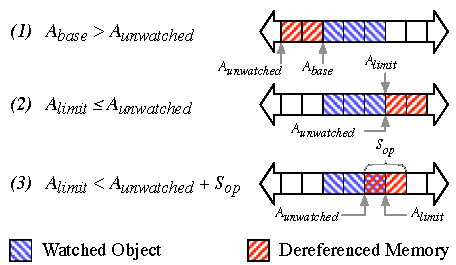
\includegraphics[width=4.5in]{overflow.pdf}
\end{center}
\iffalse
	\abovedisplayskip=0pt
	\belowdisplayskip=0pt
	\begin{align*}
		A_{base}  & > {A_{unwatched}} \tag{Underflow} \\
		A_{limit} & \leq {A_{unwatched}} \tag{Overflow} \\
		A_{limit} & < {A_{unwatched}} + S_{op} \tag{Overlap}
	\end{align*}
\fi
\caption[Buffer overflow detection]{\label{fig:detect_overflow}Three common buffer overflow cases are illustrated above: 1) underflow 2) overflow, and 3) overlap. Beside each illustration is the policy that detects the specific bug. When a watched address ($A_{watched}$) is dereferenced, a vtable function that is specific to the memory operand size ($S_{op}$) is invoked. This function detects a buffer overflow if the intended referenced memory address ($A_{unwatched}$) does not fall within the boundaries delineated by the base and the limit addresses ($A_{base}$ and $A_{limit}$, respectively).}
\end{figure}

\subsection{Type-based overflow detection\label{sec:type_overflow}}
Type-based overflow detection is applied when the type of an object is known. It is distinguished from heap-based overflow detection in that it can apply both to heap and non-heap memory, and it can be used to inform the run-time system about more accurate bounds information. In all other respects, the type-based overflow detection policy detects bugs in the same way as the heap-based policy (as might be encoded within the fields of a vector-like data structure). If the type of an object is known then it can reveal semantic relationships which can enable further type- or heap-based overflow detection. For example, the fields within a structure might encode memory bounds information (as would be the case for a vector-like data structure)

%The type-based detection policy is applied when the type of a pointer is known (i.e., not \texttt{void*}). 
The simplest use case of type information is to infer the limit address of a typed pointer. A more complex use case arises when the fields within a structure encode memory bounds information. In both cases, the vtable functions for typed and untyped memory operate in the same way.
The type of an addressable object becomes known to Granary in the context of a wrapped function. The run-time system performs a type-specific initialisation of a watchpoint's descriptor when a watchpoint is added to a pointer/address with a known type. Type-specific descriptor initialisation is a powerful feature because it allows for new watchpoints to be lazily added (thus propagating our detection capabilities) to newly discovered objects referenced \emph{within} an object of a known type. We automatically propagate type-based watchpoints using type specifications generated from parsing \texttt{C} header files. %Some manual post-processing is required if one is to inform the system of semantic relationships between function arguments or structure fields.

%use a type-specific vtable instead of a generic vtable when watching a typed pointer. Granary includes a database of 


Granary recursively follows argument and return value pointers based on object type specifications. These specifications tell Granary how to follow pointers and what--if any--pointers should be converted to watchpoints. To reduce programmer effort, Granary automatically generates type specifications and wrapper functions for any set of known types and functions. Some manual post-processing is required if the analysis/debugging application needs to understand semantic relationships between function arguments or structure fields. %\comment{Automating this process was an important goal of Granary because of Granary wraps all (approx. 6,000) exported kernel functions.}.



\subsection{Stack-based overflow detection}
Detecting stack overflows is important because they are commonly used in remote code execution and privilege-escalation attacks against operating systems \cite{SecureProgramExecFlowTracking}.
We detect overflows on stack allocated objects when memory outside of the bounds of the activation/call frame in which the object is allocated is accessed. This policy is distinguished from the heap- and type-based policies in that the watchpoint descriptor is managed separately from the watched memory, and the lifetime of the descriptor extends beyond the lifetime of the watched memory.

To detect stack overflows, we view the memory occupied by the activation frame of an invoked function as a dynamically-sized buffer. Like our other buffer overflow policies, we use a watchpoint to detect accesses to memory outside of this buffer. Unlike our other policies, we only \emph{associate} a descriptor with this buffer, and rely on a different mechanism to \emph{add} the watchpoint to stack addresses.
%, and manage what addresses are watched with this descriptor using a separate mechanism.
We separate adding watchpoints from allocating descriptors for stack overflow detection. In particular, we associate a descriptor with the buffer represented by the activation frame of a called function. This descriptor tracks the bounds of the frame over the lifetime of the function call.

We update the bounds of the frame (in the descriptor) when the frame grows or shrinks. When a function returns, the descriptor's bounds shrink to zero, but the descriptor remains allocated. We detect the two most common sources of stack overflows. First, if we see an instruction that copies the stack or frame pointers, then we assume that the copied address can escape the function. A stack address escaping a function is a potential stack-overflow risk. Adding the frame's watchpoint to this address \emph{taints} the copied address. Future copies or displacements of the watched address implicitly propagate its taintedness because offsets of a watched address reference the same descriptor. A dereference of an escaped pointer---even one happening after the function has returned---is detected as an overflow because the watchpoint descriptor remains live. Second, if we see an indexed dereference of the stack or frame pointers that uses a dynamically bound index, then we assume that the effective memory address accessed is a potential stack-overflow risk. We instrument the dereferencing instruction to add the frame's watchpoint to the effective address before the address is dereferenced.


%more support from Granary's run-time system. At a high level, each activation frame is assigned a dedicated watchpoint when a function is called. The effect of an instruction that grows or shrinks an activation frame's size is reflected by a similar change to the base address\footnote{The run-time call stack on x86 grows into lower memory.\comment{ Modifying the base address instead of the limit address allows us to maintain one set of vtable functions for all three buffer overflow detection policies.}} of the frame's watchpoint descriptor. When a function returns, the descriptor of its activation frame is cleared, but remains allocated\footnote{Reclaiming/reusing allocated but unlikey-to-be-used watchpoints is challenging. One overflow-specific approach is to ensure that the next use of the watchpoint is for a buffer whose bounds do not intersect with the current use's bounds. Another approach is to use some number of context switches as a grace period in which the watchpoint cannot be reused, but after which it can be reused. We leave this as future work.} lest the address of a local variable escape the function\footnote{If the address of a stack-allocated object escapes its function activation frame, then that pointer is said to be \emph{dangling}. Dereferences of dangling pointers can cause stack overflow errors. In the kernel, data stored in unallocated stack memory (e.g., through a dangling pointer) is at risk of being clobbered by interrupt stack frames and by function activation frames.}.  

%We assume that a memory instruction operating on a constant displacement of the stack or frame pointer registers is well-behaved. However, if the stack or frame pointer registers participate in a memory instruction and the displacement from the register is dynamically-bound then that instruction is suspect. An instruction that copies the address in the stack or frame pointer registers is also suspect because the copied address might escape the current function or participate in a local stack overflow. All suspect instructions are translated to transparently add the frame's dedicated watchpoint to the dereferenced or copied address.

%This scheme segments the runtime stack into contiguous but non-overlapping regions of watched memory. A straightforward extension excludes saved return addresses and link pointers from the known bounds of activation frames, thus detecting return-oriented buffer overflow attacks.

\begin{figure}[t]
\begin{center}
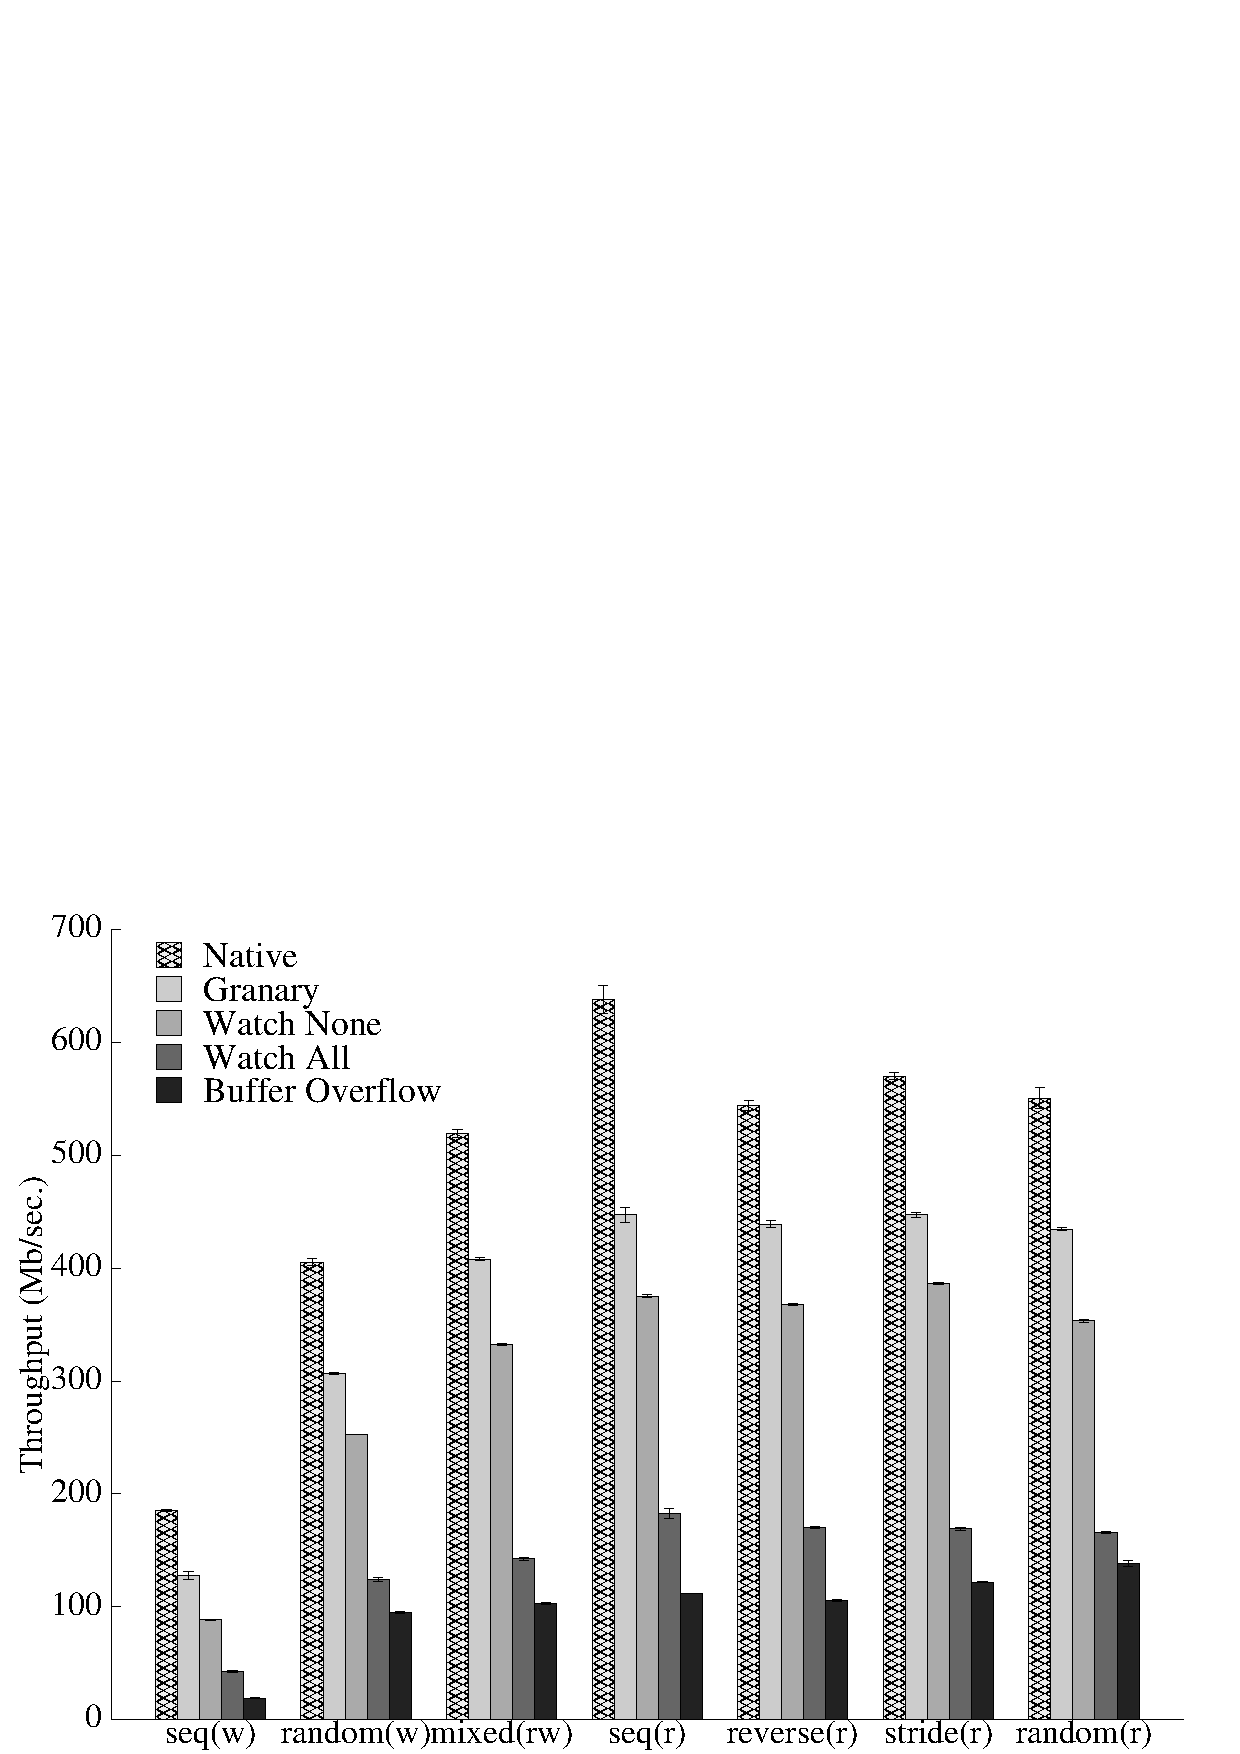
\includegraphics[width=5.0in]{watchpoint_overflow.pdf}
\end{center}
%\vspace{-15pt}
\caption[Performance impact of buffer overflow detector.]{\label{fig:watchpoint_overflow}Performance overhead (Throughput in MB/sec of common file system operations) of buffer overflow detector when used to detect the buffer overflow in \texttt{ext3} file system module. The buffer overflow detector uses code centric instrumentation for the module code and data centric instrumentation for the kernel code. The overflow detector watches all the memory allocated by the \texttt{ext3} and \texttt{jdb} modules.}
%for the watched address is shown.}
\end{figure}


\begin{table*}
\begin{center}
\begin{tabular}{|l|c c c c|}
  \hline
  Benchmark & Native & Watchpoint Null & Everything watched & Buffer overflow\\
  \hline
  Microbenchmark  & 1x & 2.7x & 3.8x & 20x\\
  \hline
\end{tabular}
\caption[Performance impact of buffer overflow detector on microbenchmark]{\label{table:overflow-benchmark}The overhead of watchpoint instrumentation for buffer overflow detector on microbenchmark shown in \Figref{microbenchmark}. The buffer overflow detector uses instrumentation for bounds checking on the access of watched objects.}
\end{center}
\end{table*}


\subsection{Evaluation}
We evaluated the performance of our buffer-overflow detector using a the synthetic microbenchmark shown in \Figref{microbenchmark} and measured the performance of common filesystem operations on an in-memory disk using the \emph{iozone} filesystem benchmark. We used the same experimental setup as described in Section~\ref{sec:approach_eval}. The overhead of the buffer-overflow detector on synthetic microbenchmark is shown in Table~\ref{table:overflow-benchmark}. The high overhead of detector is due to the instrumentation needed for precise bounds checking. \Figref{watchpoint_overflow} shows the overhead of the buffer-overflow detector on the throughput of common filesystem operations issued by the \emph{iozone} file system benchmark. We saw {\texttildelow}80\% drop in the throughput of file system operations. Much of these overhead comes because of code centric instrumentation and the overflow detector watches all the module allocated objects. Watching selected objects for buffer overflow detection will improve its performance.



%\subsection{Real World Results}
%overhead was \texttildelow 21{\footnotesize$\times$}, which is caused by the instrumentation needed for precise bounds checking.


%and measured the performance of common filesystem operations on an in-memory disk.

\section{Selective Memory Shadowing\label{sec:uninitialised_memory}}

Shadow memory enables a program analysis tool to track the history of every memory location and/or value in memory. Existing tools that use shadow memory such as Memcheck~\cite{Memcheck}, TaintCheck~\cite{NewsomeS05}, TaintTrace~\cite{Cheng:2006:TEF:1157733.1157903}, and Eraser~\cite{Savage:1997:EDD:265924.265927} demonstrate that shadow memory is a powerful and widely used method for developing program debugging applications. 


Memcheck~\cite{Memcheck} uses shadow memory to track what allocation/deallocation operations have affected each memory location, and can thus detect accesses to unaddressable memory. It also tracks the undefined memory locations (uninitialised or derived from undefined locations) and can therefore detect dangerous uses of undefined memory. TaintCheck~\cite{NewsomeS05} and TaintTrace~\cite{Cheng:2006:TEF:1157733.1157903} are security tools. They track which values are from untrusted (tainted) sources and which values were subsequently derived from them, and can thus detect dangerous uses of tainted values.
%It also remembers which values are undefined (uninitialised or derived from undefined values) and can therefore detect dangerous uses of undefined values. TaintCheck is a security tool. It remembers which values are from untrusted (tainted) sources and which values were subsequently derived from them, and can thus detect dangerous uses of tainted values.
Eraser~\cite{Savage:1997:EDD:265924.265927} uses shadow memory to track which locks are held when a memory location is accessed, and can thus detect when a memory location is accessed without a consistent lock-set, which may imply a data race. In the above applications, shadow memory provides the ability to detect critical errors, which otherwise could go undetected.

The implementation of shadow memory in these tools is inherently expensive because all memory needs to be shadowed~\cite{Nethercote:2007:SBM:1254810.1254820}. The tools need to maintain extra state for each byte of memory and instrument all loads and stores to keep this state up-to-date. These requirements increase the total amount of code that is run and the program's memory footprint, thus significantly affecting performance. Instead, behavioral watchpoints enable implementing a novel shadowing scheme that allows tracking objects selectively, which decreases the amount of code that needs to be
run and the program's memory footprint.

 %The solution of the problem associated with full memory shadowing is selective shadowing. Selective shadowing allows you to track only the objects of your interested thus decreasing the memory footprints and amount of code required to be run. 



%This makes it important to have an approach which allows you the selective memory shadowing. Selective 
%The previous work on shadow memory is mostly focused on full memory shadowing.



%is implemented in software. However implementing shadow memory correctly is hard because of following three reasons:

%First, the implementation of shadow memory is inherently expensive. A tool need to maintain large amounts of extra state and one shadow byte per byte of live original memory is typical. Most or all loads and stores must be instrumented to keep the shadow memory state up-to-date.% as must operations that affect large regions of memory, such as allocations and deallocations (on the heap or stack ), reads/writes of large areas by system calls, and the loading of the program image into memory at start-up.
%These requirements unavoidably increase the total amount of code that is run, increase a program’s memory footprint, and degrade the locality of its memory accesses. %Shadow memory tools thus typically slow down programs by a factor of 10–100, and shadow memory operations cause much more of this slow-down than other well-studied aspects of tools built with DBI frameworks such as hot trace formation [1] and code cache management [7]


%Second, The robustness of a shadow memory implementation is also important, arguably even more so than its speed. Real world tools must cope with large, uncooperative programs, and if they are to be portable, cannot rely on particular operating system characteristics such as memory layouts. Shadow memory is hard to implement robustly. The shadow memory must be squeezed into the address space alongside the
%original memory in a way that does not conflict with it and does not change the program’s behaviour. This requires considerable flexibility in the shadow memory structure and layout. It also unavoidably reduces the amount of address space a program can use itself,
%which is an important issue on embedded platforms and even 32-bit machines. Obviously, this becomes less of an issue if shadow memory
%can be made smaller, so compact shadow memory is desirable.

%In this section, we show how to use behavioral watchpoints to shadow memory. %Previous work has focused on full memory shadowing \cite{Memcheck}, while
%This section describes about the use of behavioral watchpoints in enabling \emph{selective} shadowing for watched objects. It also describes how the initialisation state of each byte of watched memory is tracked using shadow memory, and how to detect bugs related to the usage of heap-allocated memory. It also discusses the use of selective shadowing in tracking the memory access pattern of the kernel modules.

%Granary provides support to wrap kernel memory allocators and deallocators (e.g., \texttt{kmalloc}, \texttt{kfree}). Wrapped allocators add watchpoints to allocated memory, and wrapped deallocators remove watchpoints before invoking the kernel's deallocators. 
We implement selective shadow memory by maintaining a watchpoint descriptor-specific, variable-sized bitset. %\footnote{As an optimisation, shadow memory for small objects is embedded in the watchpoint descriptor.}. 
Each byte of allocated memory corresponds to one bit of descriptor-specific shadow memory. The bits in shadow memory are initialised to zero. Individual bits are flipped to one by write-specific vtable functions or read-specific vtable functions when a write/read operation happens to the bytes of memory shadowed by those bits. 

%When a wrapped allocator is invoked, a watchpoint is added to the addresses returned by those allocators
 

% in shadow memory are initialised to zero.
%Watchpoints are added to all heap-allocated objects 
%the meta-information within each watchpoint descriptor.
%By tracking the initialisation state, we detect


We use this shadow memory scheme to detect memory error bugs (e.g., uses of uninitialised memory, memory freeing bugs for heap-allocated objects) and to characterize the types of objects accessed by different kernel modules. As described in Section~\ref{sec:heap_overflow}, Granary interposes on the kernel's memory allocators and adds watchpoints to the addresses returned by those allocators. When memory is allocated, the watchpoint descriptor is initialised with the number of allocated bytes (available as an argument to the allocator) and with its own shadow memory. 

%detect uses of uninitialised memory.  Detecting such uses is important because a program using uninitialised memory can exhibit unintended, non-deterministic behaviour.

Uninitialised memory is defined as either allocated memory to which no value has been written, or deallocated memory. We selectively track the initialisation state of each byte of watched memory using \emph{shadow memory} \cite{Memcheck}. Our implementation represents shadow memory as a bitset, where the state of each bit tracks the initialisation state of a byte of watched memory. Watchpoint descriptors are augmented to include the size (in bytes) of a watched object and a pointer to the memory shadowing the object\footnote{As an optimisation, shadow memory for small objects can be embedded in the watchpoint descriptor.}.



\subsection{Read-before-write bugs}
Read-specific vtable functions detect read-before-write bugs by checking if the shadow bit corresponding to one of the read bytes is zero. However, this method of detection can report false positives: it is common for larger-than-needed reads to be performed and for compiler-added structure padding to be read (but never written). A relaxed read-before-write memory checking policy requires that at least one shadow bit is set for every read operation.

\subsection{Memory freeing bugs}
We detect freeing of non-heap memory when the argument to a kernel memory deallocator is not a watched address. We detect an invalid free, such as freeing an offset of an allocated object, when the unwatched address of a watched object being deallocated is different from the watchpoint descriptor's base address. We detect use-after-free bugs by marking the descriptor of a watched address being deallocated as dead. The lifetime of a dead descriptor extends beyond that of the object so that a later use of any watched address with that descriptor will report a use-after-free bug. We detect double-free bugs when the descriptor of a watched address being deallocated is already marked as dead.

%We use Granary to wrap the kernel's deallocation functions (e.g., \texttt{kfree}). Because all allocators are wrapped and add watchpoints, freeing of non-heap memory is easily detected when  

%We detect freeing of non-heap memory 

%If the argument to a wrapped deallocator function is a watched address then the shadow memory for the . 

%Finally, the original deallocator is invoked with the unwatched address as an argument. Reads and writes to a watched address of a deallocated object fail to pass bounds checks because the object size is zero.

Two positive side-effects of our approach is that it detects double-free bugs and freeing of non-heap memory bugs. A double-free is detected when a watched address for an already deallocated object is passed as an argument to a deallocator. An attempt to free non-heap memory is detected when an unwatched address is passed as an argument to a deallocator.

\subsection{Fine-grained access pattern}
Kernel modules execute in the kernel address space with unbounded privileges. These modules are implicitly trusted and interact with each other and the kernel through well defined interfaces and by sharing data in an uncontrolled manner. Unfortunately, the assumed trust leaves commodity OSes vulnerable to malicious and misbehaving kernel extensions\cite{BGI,LXFI, Xu:2004:DEC:1038254.1038305}. We detect the access patterns of the kernel modules using selective shadowing. Behavioral watchpoints tracks the objects of interest and any read/write access to these objects by both the kernel or the module code is captured by the shadow memory. 
The shadow memory information is logged at every control transfer from the kernel to the module. This information is useful for characterizing the access patterns of kernel modules, when may then be used to classify the module to detect module vulnerabilities.
%in a prototype and also detect the vulnerability in the kernel modules.

\section{Memory Leak Detection\label{sec:memory_leaks}}
%Memory leak is a major resource issue which could lead to the malfunctions and negative performance of the system. 
A memory leak occurs when a program does not free dynamically allocated memory or when memory can no longer be referenced. Memory leaks are especially a problem in long running programs, and in operating systems, where memory is lost until the next boot. Existing tools such as Purify~\cite{Rs_purify:fast}, Valgrind~\cite{Seward:2005:UVD:1247360.1247362} and Dr Memory~\cite{Bruening:2011:PMC:2190025.2190067} provide an effective solution for detecting memory leaks in user-space programs but they are not available for the kernel. Other systems such as \emph{kmemleak}~\cite{kmemleak} and SystemTap~\cite{EIgler05architectureof} provide support for debugging memory leaks in the kernel but they operate on the kernel as a whole and not on specific modules of interest.

%one module particularly selected by the user(s).

Implementing a leak detector only for kernel modules is challenging for three reasons. 

First, a leak detector for kernel modules should follow all objects allocated in the module context. Many of these objects should be deallocated by the module. For example, a file system module may make a call to \texttt{create\_workqueue} and allocate a \texttt{work\_struct} that can be used to schedule the delayed work. It is the responsibility of the module to deallocate the object before exit. Keeping track of such objects for a leak detector operating on the entire kernel, such as \emph{kmemleak}, is easy since they track all the memory allocation and deallocation but it is challenging for a leak detector operating only on the kernel module.  

Second, a leak detector needs to perform reachability analysis on all objects allocated in the module context to detect the lost references. Existing leak detectors use different garbage collector algorithm such as reference counting and tracing-based algorithm to detect the live objects. Performing such analysis in only module context is challenging because module regularly lose internal references to the objects that they allocate. For example, a network module can allocate objects and pass with the \texttt{net\_device} structure to the kernel, without retaining references to those objects. The network module can later indirectly access these objects using the kernel's \texttt{netdev\_priv} interface. A whole kernel leak detector, such as \emph{kmemleak}, operating on kernel heaps \& static data can detect such lost references by scanning all allocated objects but a module based leak detector, having limited knowledge of objects allocated in the module context, can not detect the references of such objects and will report them as a leak. 


Third, the existing leak detector in the kernel needs to trace all the memory allocator and deallocator functions in order to track the allocated objects. It also needs to trace the \texttt{container\_of} macros to get the addresses generated from a pre-allocated objects. \emph{kmemleak}, being tightly integrated with the kernel source code, performs this by interposing at the memory allocators/ deallocator (e.g, \texttt{kmalloc}, \texttt{vmalloc}, \texttt{kmem\_cache\_alloc} and other friend functions) and tracing the \texttt{container\_of} operations on pre-allocated objects. Performing such operations by a leak detector, having no knowledge of the kernel activities and operating only on the module binaries is not possible.


%suffers from the false negative because the allocated object doesn't maintain the state information about the memory block. This makes it difficult to identify the transient presence of freed objects in the static or the heap memory. The existing solution of leak detector based on garbage collection algorithm also can not identify the memory leaks due to the increase in stale objects. These stale objects gets allocated by the module but they never gets used and the module also doesn't lose their references. Identifying such objects without tracking the access of each memory block is not possible.


%Tracking the liveness of these objects requires a view on kernel execution which is not normally provided by module-only instrumentation.


 %are challenging because not all module-owned objects are directly allocated by modules. For example, a network driver module may make a call to an skb allocator (to allocate a \texttt{struct sk\_buff}) in an interrupt context when the module code is not running but it is the responsibility of the network module to deallocate them.



%should follow the module-owned objects and reports leak if and when module loses the reference of any of them. An object is defined as module-owned if it is allocated in the module context and it is the responsibility of the module to deallocate the object. However, keeping track of all such objects are challenging because not all module-owned objects are directly allocated by modules. For example, a network driver module may make a call to an skb allocator (to allocate a \texttt{struct sk\_buff}) in an interrupt context when the module code is not running but it is the responsibility of the network module to deallocate them.

%driver module may make a call to an skb allocator (to allocate a struct sk_buff) in an interrupt context when the module code is not running

%We built a memory leak detector for the kernel modules. The leak detector for the kernel modules follow the module owned objects and reports if module loses the references of them. A module owns the objects allocated by them and it is the module's responsibility to deallocate them. However, keeping track of all such objects is challenging because not all module-owned objects are directly allocated by modules. For example, \texttt{sk\_buff} objects used by network modules are allocated by kernel interrupt handlers, but must be deallocated by the network modules. 

%Second, a leak detector performs reachability analysis on all module-owned objects to detect the lost references of the objects. Leak detector uses different garbage collector algorithm such as reference counting and tracing-based algorithm to detect the live object. Performing such analysis in only module context is challenging because module regularly lose internal references to the objects that they own. For example, a network module can allocate objects and pass with the \texttt{net\_device} structure to the kernel, without retaining references to those objects. The network module can later indirectly access these objects using the kernel's \texttt{netdev\_priv} interface. Tracking the liveness of these objects requires a view on kernel execution which is not normally provided by module-only instrumentation.

%Third, the existing leak detector suffers from the false negative because the allocated object doesn't maintain the state information about the memory block. This makes it difficult to identify the transient presence of freed objects in the static or the heap memory. The existing solution of leak detector based on garbage collection algorithm also can not identify the memory leaks due to the increase in stale objects. These stale objects gets allocated by the module but they never gets used and the module also doesn't lose their references. Identifying such objects without tracking the access of each memory block is not possible.


 %thus the transient presence of deallocated objects in the  
%In the implementation of leak detector there is a need to track the state of the allocated objects to reduce the false negative. The existing memory allocator/deallocator doesn't maintain a meta-information with each objects. Thus making it difficult to identify the freed objects thus reporting false negative.

We implemented the leak detector for the kernel modules using the watchpoint framework. The challenges involved in implementing a leak detector only for the kernel modules make behavioral watchpoints a suitable solution. Behavioral watchpoints solve the challenges involved in three ways:
\begin{enumerate}[i)]
	\item The watchpoint framework ensures that all objects allocated in the module context are watched. These watched addresses are easily disambiguated from normal memory addresses and integers that look like watched addresses. This is done by taking over all kernel memory allocators and tracking the execution context of the module running under its control. This helps the framework identify the context of every memory allocation and adds watchpoints on all these objects. However, in the process the watchpoint framework may add watchpoints on the objects not related to the module. Adding extra watchpoints on objects does not affect the correctness of the leak detector. We detect such objects during the collector scan and suppress the false positive that may get reported due to them.

	\item Behavioral watchpoint solves the problem of losing internal reference of objects allocated in the module context by providing leak detector complete visibility of the watched objects. Any read/write accesses performed on these watched objects get detected by the watchpoint instrumentation or the hardware traps which attaches the instrumentation framework with running code. The read/ write operations on watched addresses mark these objects live and the collector scan considers these objects as reachable. The ability to track the accessed objects is particularly helpful in detecting stale objects that are potentially leaked. The leak detector based on garbage collector algorithm such as \emph{kmemleak} can not detect such objects.

	\item Behavioral watchpoints help associate the allocated object with the descriptors. The descriptors hold meta-information for each objects and help identifying the state of a memory block without much of the effort. This helps leak detector limit the scope of scanning to objects that are allocated and live. The behavioral watchpoints are also viral and every addresses derived from a watched addresses (e.g., through copying or offsetting) is also watched. The watchpoint framework does not need to trace the pointer arithmetic used to derive addresses from the allocated objects. \emph{kmemleak} reports false positive if the program uses other than \texttt{container\_of} operations to generate derived addresses. %to track the derived addresses from the% It also helps in tracking the read/write access of the watched objects by kernel or the module code.
\end{enumerate}


%Behavioral watchpoints are viral and every addresses derived from a watched addresses (e.g., through copying or offsetting) is also watched.

%Our approach ensures that all module-owned objects are watched when allocated. Leak detector ensures this by taking over all the kernel allocators and tracking every entry and exit from the kernel to the module and vice-versa. This helps us in identifying if the allocation is happening in the module context or not. We add watchpoint with all the objects allocated in the module context. 
%\texttt{call} from kernel to the module code and \texttt{ret} from the module to the kernel.   
%We ensure this by hot-patching all the kernel allocators and tracking all the calls from the module to the kernel which reaches to the allocators and add watchpoint with those objects. 
%Behavioral watchpoints solve this problem of losing the internal reference of the module-owned object by giving the leak detector visibility into kernel accesses to watched objects, which trigger hardware traps that attach instrumentation to the kernel code. This instrumentation marks kernel-accessed watched objects as live. The implementation of leak detector benefits from using watchpoints in three ways: 
%\begin{enumerate}[i)]
	%\item watched addresses are easily disambiguated from normal memory addresses and integers that look like watched addresses;
%        \item the scope of scanning can be limited using the meta-information provided by descriptors
	%\item descriptors provide meta-information that allows our system to limit the scope of scanning; and
	%\item scanning can stop if all watched objects are reached.
%\end{enumerate}




%A conventional approach of implementing leak detector is to perform the reachability analysis on the module-owned objects. The existing solution, \emph{kmemleak} uses mark/sweep algorithm \cite{Boehm:1991:MPG:113445.113459} on kernel memory to detect if/when module-owned objects become unreachable starting from a set of ``root'' objects. This is challenging because modules regularly lose internal references to the objects that they own. For example, a network module can allocate objects and pass with the \texttt{net\_device} structure to the kernel, without retaining references to those objects. The network module can later indirectly access these objects using the kernel's \texttt{netdev\_priv} interface. Tracking the liveness of these objects requires a view on kernel execution not normally provided by module-only instrumentation.

%We used behavioral watchpoints to implement memory leak detector. Our approach ensures that all module-owned objects are watched when allocated. Behavioral watchpoints solve this problem of losing the internal reference of the module-owned object by giving the leak detector visibility into kernel accesses to watched objects, which trigger hardware traps that attach instrumentation to the kernel code. This instrumentation marks kernel-accessed watched objects as live. The implementation of leak detector benefits from using watchpoints in three ways: 
%\begin{enumerate}[i)]
%	\item watched addresses are easily disambiguated from normal memory addresses and integers that look like watched addresses;
%        \item the scope of scanning can be limited using the meta-information provided by descriptors
%	\item descriptors provide meta-information that allows our system to limit the scope of scanning; and
%	\item scanning can stop if all watched objects are reached.
%\end{enumerate}

%More operationally, a dynamically-live heap object is one
%that can be reached by following pointers that will be dereferenced in the future of
%the computation (dynamically-live pointers). In order to retain only dynamically-live
%objects, the ideal garbage collector must be able to exactly identify what memory locations contain dynamically-live pointers.

\subsection{Object Liveness Analysis}\label{sec:object_liveness}
The effectiveness of a leak detector in identifying the object leaks depend on the ``accuracy'' of the liveness analysis. An ideal leak detector identifies all heap-allocated objects that are not dynamically live and reports them as leak. A dynamically-live heap object is one that can be reached by following pointers that may be dereferenced in the future. 

Existing leak detector solutions such as \emph{kmemleak}~\cite{kmemleak}, Purify \cite{Rs_purify:fast} and Dr Memory \cite{Bruening:2011:PMC:2190025.2190067} use a garbage collection algorithm to perform object liveness analysis. They use the mark/sweep collector algorithm \cite{Boehm:1991:MPG:113445.113459} to detect reachability of the allocated objects starting from a set of ``root-set'' objects. Their root-set includes system registers and non-heap addressable memory. 

They perform reachability analysis periodically at intermediate position and it involves stopping the client when collector\footnote{A low priority daemon thread which runs intermittently in the background performing reachability analysis on the allocated objects} is in process. However, the solution is not very efficient when client operates on a large number of heap-allocated objects, such as is typical in operating systems. It stops the client for longer time. 

One solution for reducing the pause time is to use generational or parallel collection. Generational collection avoids stop-the-world by running the collector thread occasionally but it doesn't remove the problem completely. However the parallel collectors take an orthogonal approach and reduce the time of pause by running the collector in parallel to the client.


In our implementation of leak detector we used the parallel collector to perform object liveness analysis. Keeping in view of the challenges involved in performing object liveness analysis, we used three different policies to perform the leak scan. 

%took middle approach and used mostly-parallel collector~\cite{Boehm:1991:MPG:113445.113459, Barabash:2005:PIM:1108970.1108972} to perform the object liveness analysis. It is called as mostly parallel collector because we update the ``root-set'' in stop the world collector and perform the reachability analysis from these ``root-sets'' by running the collector parallel to mutator (client). 
%The aim of our leak detector is to detect the memory leaks in the kernel modules. These kernel modules execute in a complex and dynamic environment, sharing the data over irregular interface. Many of these shared objects are allocated directly or indirectly by the modules. Behavioral watchpoints provide an efficient solution by providing complete visibility to the module-owned object and making these watched objects easily identifiable, thus limiting the scan space but they does not provide any solution for performing the reachability analysis on all these watched objects. Performing reachability analysis on these objects is challenging because of two reasons. First, these module allocated objects get shared with the kernel over complex and irregular interface making them difficult to track and many of them are reachable only through the kernel internal data structure. The reachability analysis of these objects without accounting the kernel allocated memory is non-trivial and it will lead to false positives. Second, our leak detector framework gets loaded as the kernel modules and it comes into the picture long time after the system ``boot-up''. Without having account of these memory block we can not claim to perform the complete leak scan. Keeping in view of these challenges we used three different policy for performing the leak scan. 


%A conventional approach of implementing leak detector is to perform the liveness analysis on the allocated objects. Existing solution such as \emph{kmemleak}~\cite{kmemleak}, Purify \cite{Rs_purify:fast} and Dr Memory \cite{Bruening:2011:PMC:2190025.2190067} uses garbage collection algorithm to perform object liveness analysis. \emph{Kmemleak} uses mark/sweep algorithm \cite{Boehm:1991:MPG:113445.113459} on kernel memory to detect the reachability of the allocated objects starting from a set of ``root'' objects. The effectiveness of leak detector in identifying the lost objects depends on the accuracy of their object liveness analysis. 
%Existing solution such as Purify \cite{Rs_purify:fast} and Dr Memory \cite{Bruening:2011:PMC:2190025.2190067} leak detector uses garbage collection algorithm to perform liveness analysis. 
%A straightforward implementation of garbage collection algorithm is to implement tracing based collector. It involves stopping the client when collector is in the process performing liveness-analysis. However, this solution is not very efficient when client operates on very large heap-memory as it stops the clients for longer time. The solution to reduce the pause time in tracing algorithm based leak detector is generational or parallel collection. Generational collection avoids stop-the-world time by running the collector thread occasionally, thus doesn't remove the problem completely. However the parallel collectors takes orthogonal approach and reduces the time of pause by running collector parallel to client. We took similar approach of mostly-parallel collector to perform the object liveness analysis.

%In Linux kernel, the module and kernel interacts in a complex ways and there is frequent transfer of shared objects between the kernel and the modules. Many of these shared objects are allocated by the module. Keeping track of the references of these objects with only module view of the objects is non-trivial. This makes it important for the leak detector to track both kernel and the module objects. It was important for us to study the transfer or the ownership of the objects. In our implementation of leak detector we uses three different scan policy to perform the object liveness analysis.

 %following three different liveness analysis policy for the leak detector:

\paragraph{Scanning of accessed objects:} This is an aggressive scanning policy for detecting memory leaks. The approach is similar to bookmarking collectors~\cite{Hertz:2005:GCW:1065010.1065028} and Melt~\cite{Bond:2008:TML:1449764.1449774} which track the accesses of allocated memory blocks to detect stale objects at page or object granularity. The approach considers all objects that are accessed between two consecutive scans as live objects and performs reachability analysis considering them as ``root-sets''. Any object which is not reachable from these objects is considered as stale or a potentially leaked object. 

The leak detector tracks all accesses of the watched objects and updates the meta-information associated with their descriptors. The scanner thread (collector) periodically scans the descriptors stored in a global descriptor table and marks the objects that were accessed in the last epoch as live. The scanner thread later performs reachability analysis considering these objects as ``root-sets''.  The leak detector also tracks the sources of memory allocation in the descriptors and a constant increase in the stale objects from one source is reported a possible leak.


This approach reduces the overhead of leak scan which is performed by the collector periodically and it is also helpful in finding stale objects (dead but reachable) which the existing garbage collector algorithm based leak detector can not detect. However, the approach performs limited reachability analysis, thus resulting in increase in the false positive especially for objects which does not get accessed for longer interval of time. It also can't find the objects with live leak i.e the allocated objects are getting accessed periodically but these accesses are nonetheless useless. Detecting such leaks with any leak detector is challenging.



 %to find the objects which is accessed in last epoch and mark them dead accounting them as live during the scan interval. The approach also tracks the source of each allocation and the constant increase in the stale objects from one source increase the possibility of memory leaks. 

%In this scan policy, every access of the watchpoint objects also updates the meta-information associated with them. The scanner thread periodically scans the descriptor to find the objects which is accessed in last epoch and mark them dead accounting them as live during the scan interval. The approach also tracks the source of each allocation and the constant increase in the stale objects from one source increase the possibility of memory leaks.

%The approach decreases the cost of performing object liveness analysis by the collector and it is also helpful in finding the leaks of stale objects (dead but reachable) which can not be identified using garbage collector algorithm. However, the approach is limited in performing reachability analysis, thus it results in the false positive especially for the objects which doesn't get accessed for long interval of time. The approach also can't find the objects with live leak where the allocated objects gets accessed periodically but these accesses are nonetheless useless. Detecting such leaks in the module is difficult.


%and mark them dead after accounting them as live during the scan interval. The leak detector makes decision after 10 scans.

%The approach deceases the cost of object liveness analysis, but it results in the false positive for those objects which doesn't gets accessed for long period of time.

\paragraph{Scanning of module reachable objects:} 
We define module reachable objects as objects which a module can access directly or has accessed in the past. It includes static data for both the kernel and the modules, system registers, threads stack executing module code and all heap-allocated memory viewed by the module directly or indirectly. Module viewed objects are the objects allocated by the kernel but passed to the module during its course of execution. We keep track of such objects by interposing at the kernel/module interface and collecting all the kernel objects passed to the modules. The type information about these objects helps us in associating a type-specific scanner with each object, which performs deep scanning of these objects during a leak scan.

In this leak scan policy, the collector considers all module reachable objects as the ``root-set'' and recursively scans them to perform liveness analysis. This scan policy uses the mostly-parallel collector~\cite{Boehm:1991:MPG:113445.113459, Barabash:2005:PIM:1108970.1108972} instead of the parallel collector for updating the ``root-set'' before performing the leak scan. This is important to have a consistent snapshot of system registers and thread stack running the module code.  The parallel scanning of kernel objects requires maintaining consistency and avoid the cyclic dependency of dependencies across data structures. We detect cyclic dependencies by hashing each memory block during a scan and storing them in a data structure. The scan of a memory block is stopped if its hash is found. We also use the scan depth as a fall back mechanism to avoid walking a long list of objects in a data structure. In our implementation we used a scan depth of ``6'' which we find is appropriate for detecting all watched objects in any kernel data structure. We are also using relaxed consistency policy during the scan. This is because our leak detector makes a decision about a memory block leak after multiple scans.

This approach reduces false positives compared to the first approach because it includes module-viewed objects in the root set. However, it has a higher cost because it requires maintaining bookkeeping information for the module-viewed objects and tracking their deallocation. The approach does not remove false positives completely as it is not able to track references to objects that are allocated by the module but passed to the kernel, after which the kernel uses internal data structures to maintain references to the objects.

%kernel and kernel uses internal data structure to maintain its references. 

%of object scan by scanning them twice before making a decision. We consider our consistency approach an appropriate because the leak detector makes decision about a memory block after multiple scans.

%where the ``root-sets'' for scan gets updated in stop-the-world collector. This is required to have a consistent snapshot of system registers and thread's stack running the module code. The parallel scan of kernel objects requires to maintain consistency and avoid the cyclic dependency of data structure. We avoid the cyclic dependency by hashing the memory block after every scan and storing them in a data structure. The scan of a memory block gets suspend if its hash is found in the data structure. We also use scan depth as the fall back to avoid walking of the list objects in a data structure. In our implementation we used the scan depth as ``6'' which we find appropriate for detecting the watched objects in the data structure. We relaxed the consistency of object scan by scanning them twice before making a decision. We consider our consistency approach an appropriate because the leak detector makes decision about a memory block after multiple scans.




%The module reachable objects includes the static data for both the kernel and modules, system registers, stack of threads executing module code and all heap-allocated memory viewed directly or indirectly by the module. We defined the module viewed objects as the objects allocated by the kernel but passed to the module during its course of execution. We keep track of all such objects by interposing at the kernel/module interface and each object gets associated with a corresponding type scanner function based on the object types. These type scanner function is used by the collector to recursively scan the object.

%This scanning policy uses mostly-parallel collector where the ``root-sets'' for scan gets updated in stop-the-world collector. This is required to have a consistent snapshot of system registers and thread's stack running the module code. The parallel scan of kernel objects requires to maintain consistency and avoid the cyclic dependency of data structure. We avoid the cyclic dependency by hashing the memory block after every scan and storing them in a data structure. The scan of a memory block gets suspend if its hash is found in the data structure. We also use scan depth as the fall back to avoid walking of the list objects in a data structure. In our implementation we used the scan depth as ``6'' which we find appropriate for detecting the watched objects in the data structure. We relaxed the consistency of object scan by scanning them twice before making a decision. We consider our consistency approach an appropriate because the leak detector makes decision about a memory block after multiple scans.

%The approach decreases the false positive by including the module viewed kernel objects in the ``root-sets''. However, the approach requires to maintain book-keeping of kernel objects passed to the module which has additional cost. The approach also doesn't remove the false positive completely as it is not able to track the references of objects which are allocated by the module but passed to the kernel and kernel uses local data structure to maintain its references. 


%the state data of both the kernel and modules and all the kernel and module heap-allocated object which is viewed directly or indirectly by the module.

%In the initial implementation of leak detector, we decided to track all the in-memory kernel data structure. we track all the module viewed objects. We defined the module viewed objects as the objects passed to the module during its course of execution. We keep track of all such objects and scan them periodically looking for the watchpoints. To maintain the consistency during the data structure we scan them twice and to avoid the circular dependency on the data structure we hash the data structure.

%This policy decreases the false positive but requires to have a lot of book-keeping for the kernel objects. The approach is also not able to track the references of objects which are allocated by the module but passed to the kernel and kernel uses local data structure to maintain the reference of the objects for long time. 

%we studied the ownership transfer of the module owned objects. We track all the object viewed by the module and scan them periodically looking for the watchpoints.





\paragraph{Scanning of kernel heaps and static data:} This is the most conservative policy and used as the fall back approach for performing a leak scan. This policy scans the static data for both kernel and the modules and kernel heaps to find any references to watched objects. A watched object that is not found during the scan is definitely considered a leak.

For scanning kernel pages, we used the kernel page tables and the kernel data structure \texttt{init\_level4\_pgt} to access kernel pages. The scanner thread (collector) divides the kernel pages based on the memory regions and types and scans them based on priority. The scanner thread stops scanning the kernel pages once it finds at-least one reference to watched objects.

This approach avoids any false positives but scanning the kernel heap memory is expensive. Also, the scanning of kernel pages can cause false negatives because leaked objects may have internal pointers containing watched addresses. We reduced the problem by removing the memory block of watched objects that are not live from the scan list.


 %and pointers associated with kernel data structure which is not zeroed out. 


%We reduce the false negative by ignoring the scan of pages associated with watched object and they get scanned only when a reference of that object is found in other pages. This is particularity required as we found in many cases the internal pointers of watched object was initialized with the watchpoint address and scanning of these pages or memory block will provide the false negative even if the object is considered as lost. 

%for implementing leak detector. In this policy we scan the entire kernel heap and module \& kernel static data for finding the references of the watchpoints. Any watchpoints not found during the scan is considered as leak. For scanning the kernel heaps and static data structure we walk over the kernel page table using the page table data structure \texttt{init\_level4\_page}.

%The scanning the kernel heap and static data reduces the chances of false positive but the cost of scanning them is costly. However, In our approach we device the kernel address space in different region and we scan them based on the priority. The scanner thread also stops scanning the memory once it finds at least one reference of all the watched objects.

%The disadvantage of scanning the kernel heaps is that 

%In this can policy we scan the entire heap memory and static data by walking over the page table looking for the watched objects.


%Other solutions such as (...) considers objects staleness as an indicator of problematic behavior.


%The existing leak detector tracks the behavior of the arbitrary objects   

%track behaviors
%of arbitrary objects and report problems when tracked objects
%become suspicious. One major category of work [8, 9, 10, 18, 33]
%considers objects’ staleness (i.e., time elapsed since the program
%last used these objects) as an indicator of problematic behavior,
%while another category [20, 23] treats objects as suspicious if instances
%of their types exhibit sustained growth

%Our approach of leak detector is based on the liveness analysis of heap objects, which are directly or indirectly allocated by the modules. Similar to existing solution like Purify \cite{Rs_purify:fast} and Dr Memory \cite{Bruening:2011:PMC:2190025.2190067}, leak detector uses garbage collection algorithm to detect memory leaks. A straightforward implementation of garbage collection algorithm is to implement tracing based collector. It involves stopping the client when collector is in the process performing liveness-analysis. However, this solution is not very efficient when client operates on very large heap-memory as it stops the clients for longer time. The solution to reduce the pause time in tracing algorithm based leak detector is generational or parallel collection. Generational collection avoids stop-the-world time by running the collector thread occasionally, thus doesn't remove the problem completely. However the parallel collectors takes orthogonal approach and reduces the time of pause by running collector parallel to client. We took similar approach of mostly-parallel collector to perform the object liveness analysis.  

%In our approach of liveness analysis, we use three different analysis policy:



%The leak detector scans kernel memory using the conventional mark/sweep algorithm \cite{Boehm:1991:MPG:113445.113459} to detect if/when module-owned objects become unreachable starting from a set of ``root'' objects. This is challenging because modules regularly lose internal references to the objects that they own. For example, a network module can allocate objects and pass with the \texttt{net\_device} structure to the kernel, without retaining references to those objects. The network module can later indirectly access these objects using the kernel's \texttt{netdev\_priv} interface. Tracking the liveness of these objects requires a view on kernel execution not normally provided by module-only instrumentation. Behavioral watchpoints solve this problem by giving the leak detector visibility into kernel accesses to watched objects, which trigger hardware traps that attach instrumentation to the kernel code. This instrumentation marks kernel-accessed watched objects as live.



%The leak detector benefits from using watchpoints in three ways: %\begin{inparaenum}[i)]
%	\item watched addresses are easily disambiguated from normal memory addresses and integers that look like watched addresses;
%        \item the scope of scanning can be limited using the meta-information provided by descriptors
%	\item descriptors provide meta-information that allows our system to limit the scope of scanning; and
%	\item scanning can stop if all watched objects are reached.
%\end{inparaenum}

%Two key benefits of our watchpoints solution is that watched addresses are easily disambiguated from normal memory addresses, and that we can stop scanning memory if all watched objects are live and reachable.

%Detecting leaks of such objects with a limited view of module is challenging. Behavioral watchpoints provide a way to ensure the visibility of such objects by triggering a hardware trap on its access and mark them as live.
%on memory access of these objects by enabling demand-based translation and marking them as live.


% during device registration. 


%The object becomes invisible to the module and gets accessed through the kernel interface \texttt{netdev\_priv}. This makes it difficult to detect leaks based on module's limited view. Bhavioural watchpoints provides a way to ensure complete visibility on memory access of these objects by enabling demand-based translation and marking them as live.

%All module owned objects are not directly allocated by the module and kernel can allocate it on behalf of the module. 
%All module-owned objects are not directly allocated by the module. For example, a network driver module may make a call to an skb allocator (to allocate a \texttt{sk\_buff} structure) in an interrupt context. Once the buffer is send over the network, it is the responsibility of the network module to deallocate the buffer. In Granary, we use wrappers to add watchpoints at relevant allocators such as \texttt{\_\_alloc\_skb}. The leak detector keeps track of these watched objects and reports possible leaks. 

%Module holds partial view of the kernel and to detect leaked object there is a need to perform reachability analysis on both kernel and module objects. Behavioral watchpoints helps in identifying the objects owned by the module, thus limiting the type of objects which needs to be tracked. Watched object holds descriptor information in high-order bits, making it easy to track the memory state information. This is helpful in identifying live objects and reduces the chance of false positive. The leak detector uses the conventional mark and sweep algorithm and mostly-parallel collector~\cite{Boehm:1991:MPG:113445.113459} to perform the rechability analysis.
 
%Watched addresses are also more easily disambiguated 

%Behavioral watchpoints are important for implementing the leak detector because they help in identifying the objects owned by the module, thus limiting the type of objects that need to be tracked. Each watched object holds the memory state information embedded in its descriptor, making it easy to identify objects that are live and reachable. % from one of the root-sets\footnote{The root-set for leak detector reachability-analysis includes both kernel and module data structures.}. 
%The leak detector uses the conventional mark and sweep algorithm and mostly-parallel collector~\cite{Boehm:1991:MPG:113445.113459} to perform the reachability analysis.


%are easily identifiable because they hold the descriptor table index in high-order bits and 3) Each watched object holds the memory state information with it. Thus making it easy to identify the the objects which are live and reachable from one of the root-sets. The leak detector uses the conventional mark and sweep algorithm and mostly-parallel collector~\cite{Boehm:1991:MPG:113445.113459} to perform the rechability analysis.



%there is a need to perform rechability analysis of all kernel objects, which will have significant cost.



%then gets accessed through the kernel interface and become invisible to the module and is reachable only through the \texttt{net\_device} structure. Bhavioural watchpoints ensures complete visibility of these objects and enables on-demand instrumentation on its access, marking them live.



%Developing a leak detector only for kernel modules is challenging because of following three reasons:
%Our approach is based on performing reachability analysis on module owned objects. 
%Memory leak is a common problem in Linux kernel and its modules \cite{Boehm96simplegarbage-collector-safety}. A serious memory leak in kernel modules can easily make the system unstable this is because every time kernel losses a piece of memory, it can't be reclaimed until next boot. 
%Our approach of detecting memory leaks in kernel module is to perform rechability analysis on the module owned objects. 
%This is challenging because: 

%1) All module owned objects are not directly allocated by the module. For example, a network driver module may make a call to an skb allocator (to allocate a \texttt{sk\_buff} structure) in an interrupt context when the module code is not running. Once the buffer is send over the network, it is the responsibility of the network module to deallocate the buffer.

%2) Module allocates many independent objects which they share with the kernel. Module losses its visibility once such objects are passed to the kernel. For example, a network module during device registration can allocate an object and pass it with \texttt{net\_device} structure. This object then become invisible to the module and is reachable only through the \texttt{net\_device} structure. Detecting leak for such objects requires complete visibility of the kernel. 
%an object and pass it with \texttt{net\_device} structure. 
%till it gets its reference 
% passed to the kernel till it gets his reference back. 
%frequently share with the kernel. Module looses the visibility for such objects till it gets back their references. For example, filesystem module \texttt{ext3} allocates object of type \texttt{inode} and passes it to the kernel. The module holds no reference of the object once it is passed and only 
%loose its visibility for module code till the time kernel passes them back to the module. For example,   
%There is frequent transfer of module allocated objects at kernel/module interface and module may not hold the reference of objects passed to the kernel.  For example, file-system module \texttt{ext3} allocates object of type \texttt{struct inode} and passes it to the kernel. Once it is passed to the kernel module doesn't hold reference of \texttt{struct inode}. Thus having limited view of the module doesn't help in detecting leaks.  

%3) Module only holds partial view of the kernel and much of the module allocated objects are reachable only through the kernel objects. To detect the leaked object there is a need to perform rechability analysis of all kernel objects, which will have significant cost.


%and detect the leaked objects it is needed to perform the rechability analysis on 


%In Granary, we use wrappers to add watchpoints to the relevant allocators (e.g., \texttt{\_\_alloc\_skb, skb\_clone}). The leak detector keeps track of these watched objects and reports possible leak. 

%Behavioral watchpoints are important for implementing the leak detector because: 1) They help in identifying the objects owned by the module, thus limiting the type of objects which needs to be tracked, 2) The watched addresses are easily identifiable because they hold the descriptor table index in high-order bits and 3) Each watched object holds the memory state information with it. Thus making it easy to identify the the objects which are live and reachable from one of the root-sets. The leak detector uses the conventional mark and sweep algorithm and mostly-parallel collector~\cite{Boehm:1991:MPG:113445.113459} to perform the rechability analysis. % from its root-sets. 
%Based on this leak detector divides the watchpoints into three different categories: 
%\begin{enumerate*}
%   \item[i)] Watched objects which are reachable from one of its rootset. They are not considered as leak.  
%   \item[ii)] Watched objects that are not reachable from any of the rootsets are considered as potentially garbage. 

   %Watched objects that are not reachable and never owned by the modules are considered as live. This include objects which are allocated in the module context but never reached to the module. Leak detector keeps tracks of such objects by for further analysis.
    %These includes objects which are allocated in module context but are not owned by the modules. Leak detector keep tracks of such objects by marking them as live. 
%   \item[iii)] Module owned objects that are not reachable from any of the rootsets are considered as potentially garbage. 

   %Determining the garbage objects with partial view of kernel and scanning of kernel objects passed to the module is challenging. However, to detemine this we follow the ownship history of the objects and any watched objects which is owned by the modules previous and are not rechable from any of the root-sets is reported as leak. Root-sets are set of object references which are prior reachable and for our leak detector it includes kernel and module static data and kernel objects passed to the module.  
%\end{enumerate*}


%in performing reachability analysis, as the addresses are identifiable and it stores the state of a memory 



%allocation of \texttt{struct sk_buff} in interrupted context and it is the responsibility of the module to deallocate it.  


%call \texttt{__alloc_skb} in interrupted context to allocated sk


%which is passed to the module.    


%Leak detector identifies the module ownership of an object based on its context of allocation and access pattern. Performing rechability-analysis on these objects are challenging because not all module owned objects are directly allocated by them. Granary identifies the


%The module ownership of an object is identified by its context of allocation and access pattern. 

%Behavioral watchpoints track the ownership of an object by identifying its source of allocation and access pattern.


%However, 


%this is challenging because not all objects owned by the module are directly allocated by them.   

%Every time kernel losses a piece of memory, it is gone until the next boot and a serious memory leak in the kernel modules can easily make the system unstable. One method of detecting memory leak in kernel modules is to perform rechability analysis on all allocated objects. This is challenging because not all module owned objects are directly allocated by the module and there is frequent transfer in ownership of the objects at kernel/module interface.

%Behavioral watchpoints track the ownership of an object by identifying its source of allocation and access pattern. To detect the memory leak, Leak detector performs rechability-based analysis only on the objects owned by the module. Study of object ownership also helps in fixing the responsibility for deallocating the object and any default in this is considered as memory leak.

%We use Granary to wrap the kernel’s memory allocator functions (e.g., \texttt{\_\_kmalloc}) and add watchpoints to the objects allocated in the module context. It decides this based on the call graph of the allocator functions. Granary also tracks the kernel objects passed to the module at interface and mark them as module known objects. Leak detector use these module known objects along with kernel and module static data as rootset to perform rechability analysis. Other alternative for rechability-analysis is to scan entire kernel heap.  

%Granary also keeps track of all the objects passed to the module at interface and cosiders them as root-set to perform reachability analysis. However, this approach provides leak detector limited view of the kernel and based on that it divides the allocated objects into three categories:
%\begin{enumerate*}
   %\item[i)] Module owned objects that are live and rechable from one of the prior roots are not considerd as leak. 
   %\item[ii)] Watched objects that are not reachable and never owned by the modules are considered as live. This include objects which are allocated in the module context but never reached to the module. Leak detector keeps tracks of such objects by for further analysis.
    %These includes objects which are allocated in module context but are not owned by the modules. Leak detector keep tracks of such objects by marking them as live. 
   %\item[iii)] Module owned objects that are not reachable from any of the rootsets are considered as potentially garbage. 

   %Determining the garbage objects with partial view of kernel and scanning of kernel objects passed to the module is challenging. However, to detemine this we follow the ownship history of the objects and any watched objects which is owned by the modules previous and are not rechable from any of the root-sets is reported as leak. Root-sets are set of object references which are prior reachable and for our leak detector it includes kernel and module static data and kernel objects passed to the module.  
%\end{enumerate*}

%for the module-owned objects.    




%is to perform the rechability analysis on all kernel allocated objects. 

%Memory leak bugs are a common problem with C and C++ based applications \cite{Boehm96simplegarbage-collector-safety}. These bugs are difficult to identify or track-down without the help of a dedicated tool \cite{Memcheck, Bruening:2011:PMC:2190025.2190067}. Memory leak can be a problem especially in long running application and is worse in the kernel because every time a piece of memory is lost, it is gone until the next boot.
%Memory leaks can be a problem in applications, especially those which run for a long time
%Memory leak bugs are common in Linux kernel and its modules which are mostly developed in C. These bugs are difficult to identify or track-down without the help of a dedicated tool. 
%Memory leaks in kernel is worse because of its long running nature and every time a piece of memory is lost, it is gone until the next boot. 
%Linux kernel modules works as an extension of Operating system providing additional features, while running in the privilege mode and a serious memory leak in the kernel modules can make the operating system unstable. In this section we will describe our approach of using behavioral watchpoints in detecting memory leak bugs in kernel modules.

%\paragraph{Liveness Analysis} Our approch of leak detector is based on the liveness analysis of heap objects, which are directly or indirectly allocated by the modules. Similar to existing solution like Purify \cite{Rs_purify:fast} and Dr Memory \cite{Bruening:2011:PMC:2190025.2190067}, leak detector uses garbage collection algorithm to detect memory leaks. %Behavioral Watchpoints being able to hold context-specific information with each objects and are equally efficient for both the methods
%It uses conventional mark and sweep algorithm and recursively follows potential pointers from the data, stack segment and heaps to mark the objects live and reachable. Many implementation of mark and sweep based tracing algorithm exist and a straightforward implementation invloves stopping the client(mutator) to perform the liveness analysis. This solution is not very efficient when client operates on very large heap-memory as it will increase the pause-time and touching heap memory will blow away the cache, seriously affecting the system performance. One solution to reduce the pause time is using generational collection based algorithm. However, this avoids the problem by scheduling the collector thread less frequently, thus doesn't remove the problem completely. In our leak detector we remove this problem by using mostly parallel collector. Mostly-parallel collectors takes an orthogonal approach and reduces the problem by having collector doing most of the work parallel to the client and using stop-the-world to prepare the system. 


%running collector parallel to client

%However this doesn't completely remove the 


%. The solution to reduce the pause time in tracing algorithm based leak detector is generational or parallel collection. Generational collection avoids stop-the-world time by running the collector thread occasionally, thus doesn't remove the problem completely. However the parallel collectors takes orthogonal approach and reduces the time of pause by running collector parallel to client. We took similar approach of mostly-parallel collector to perform the object liveness analysis.  




%A straigntforward implementation of tracing based collector involves stoping the client when collector is in the process performing liveness-analysis. This solution is not very efficient when client operates on very large heap-memory as it stops the clients for longer time. The solution to reduce the pause time in tracing algorithm based leak detector is generational or parallel collection. Generational collection avoids stop-the-world time by running the collector thread occasionally, thus doesn't remove the problem completely. However the parallel collectors takes orthogonal approach and reduces the time of pause by running collector parallel to client. We took similar approach of mostly-parallel collector to perform the object liveness analysis.  


%purify uses an algorithm similar to the conventional mark and sweep. In the mark
%phase,i lyify-recursively follows potential pointers from the data and stack segmentsin to the heap and marks all
%blocks referencedin the standard"conservativea"n d "pessimistic" 

%embed context-specific information with each objects and are equally efficient for implementing both direct and indirect method of leak detection but we decided to use the tracing algorithm which has no overhead cost for maintaining and updating the records for each objects.



%both direct and indirect method of leak detection but we decided to use the tracing algorithm which has no overhead cost for maintaining and updating the records for each objects.


%The existing solution for memory leak detection uses two methods to perform livness analysis: the reference counting \cite{Maebe_precisedetection} and tracing methods \cite{Bruening:2011:PMC:2190025.2190067}. 


%The existing solution for memory leak detection uses two methods to perform the liveness analysis: the direct method and the indirect method. Direct method requires that a record be associated with each object in the heap on behalf of the objects which gets updated based on if a pointer is set to refer to this object or the reference of the object is lost. Reference counting is one of the common direct method for detecting leaks. The indirect method includes the tracing algorithm where the live-ness analysis is performed at later point of time independent of client. Behavioral Watchpoints embed context-specific information with each objects and are equally efficient for implementing both direct and indirect method of leak detection but we decided to use the tracing algorithm which has no overhead cost for maintaining and updating the records for each objects.
%
%\paragraph{Leak Scan}
%A common tracing algorithm used to implement garbage collector is mark-and-sweep operation. We used similar method to perform the liveness analysis on module allocated objects. A straigntforward implementation of tracing based collector involves stoping the client when collector is in the process performing liveness-analysis. This solution is not very efficient when client operates on very large heap-memory as it stops the clients for longer time. The solution to reduce the pause time in tracing algorithm based leak detector is generational or parallel collection. Generational collection avoids stop-the-world time by running the collector thread occasionally, thus doesn't remove the problem completely. However the parallel collectors takes orthogonal approach and reduces the time of pause by running collector parallel to client. We took similar approach of mostly-parallel collector to perform the object liveness analysis.  

\paragraph{Types of Leaks}
The three scanning policies for performing liveness analysis on watched objects detect leaks at different levels. Based on the leaks reported by these policies, the detector divides allocated memory objects into three categories:
%Implementing memory leak detector for kernel modules without having full knowledge of kernel is non-trivial. This is because not all module owned objects are directly allocated by the module and there is frequent change in the ownership of the objects at kernel/module interface. Leak detector makes use of wrapper interface of Granary to add watchpoints with all the objects allocated in module context and lazily tracks their ownership at collection. This is particularly important to reduce the false positive. However, our approach of lazily determining object ownership require us to keep track of all the objects passed to the modules but this avoids the scanning of kernel heaps for liveness-analysis. Based on limited kernel view and lazy collection of objects allocated by the modules, leak detector divides them into three categories: 
\begin{enumerate}
   \item[i)] Live objects: These objects have been accessed between leak scans and are thus live and reachable from one of the roots. Objects are marked live after the scanning of accessed objects
   %Objects that are definitely live and reachable from one of the roots. It includes the objects which is getting accessed between the different leak scans. These objects are not stale and can not be considered as leak. The decision about such objects are made after scanning of the accessed objects.
   \item[ii)] Stale objects: These objects have not been accessed for a small number of scans but there is a possibility that they are live. Objects are marked as stale after the scanning of module reachable objects. The decision about these objects are made after performing the full system scan of kernel heaps and static data.
   %Objects that are stale but potentially live. These include objects that do not get accessed for a longer period of time, but there is still a possibility for such objects to be live. An object is moved into this category if it doesn't get accessed for a long period of time but it is not causing memory bloat. The decision about the leak of such objects is taken after scanning the module reachable objects or performing the full system scan of kernel heaps and static data.
   %of such type is not causing the memory bloat. If there is a memory bloat due to the staleness of such objects it is reported as leaked objects. %which are allocated in module context but are not owned by the modules. Leak detector keep tracks of such objects by marking them as live. 
   \item[iii)] Garbage objects: Objects that are not reachable and are certainly garbage. The decision about such objects is made after scanning the kernel heaps and static data of the kernel and its module. 


   %Determining the garbage objects with partial view of kernel and scanning of kernel objects passed to the module is challenging. However, to determine this we follow the own ship history of the objects and any watched objects which is owned by the modules previous and are not reachable from any of the root-sets is reported as leak. Root-sets are set of object references which are prior reachable and for our leak detector it includes kernel and module static data and kernel objects passed to the module.  
\end{enumerate}

\paragraph{Meta-information}
The leak detector maintains two kinds of meta-information to track the state of a memory block and to detect leaked objects. This meta-information is added in the descriptor of an object. % whose index gets embedded  with the watchpoint. 
%The analysis requires maintenance of two kinds of metadata. First is the record of the segments in the program, each of which has the following form.
\begin{itemize}
\item \emph{leak\_state :} This includes the state of the memory block. It tracks if the memory is allocated and is accessed in the last epoch. It also counts the number of epochs since the object not been accessed. Our current implementation of the leak detector is aggressive and it performs a full system scan for an object if it does not get accessed in the last two epochs.
%It tracks if the memory is being accessed in last epoch and it also counts the number of epochs since the memory is not accessed.
%\item \emph{source :} This includes the source of allocation and type of allocator used for allocating the memory block and the call-stack for the allocation.
\item \emph{memory\_info :} This includes basic information about a memory blocks such as base address, size and type and source of allocation.
\end{itemize}

%X, a segment-type, describes a segment; this includes its base address, size, location (heap,
%stack, or static), and status (in-use or freed).

%Each segment is given a segment-type X.
%Second is the location metadata shadowing each register and memory word, describing the runtime
%type of the word. This metadata has one of the following three forms.

%n, a non-pointer-type, describes a value which is known to be a non-pointer.
%p(X), a pointer-type, describes a value which is known to be a pointer to a segment X.
%u, an unknown-type, describes a value for which the type is unknown.
%Each word-sized value is shadowed by one of n, u or p(X). In principle, every value produced, of
%any size, can be assigned a type. In practice, the shadow value tracking can be done at word-sized
%granularity because all memory accesses are through word-sized pointers.
%A root-set is de-
%fined by the set of references of objects which are prior
%reachable. 



%These are the objects that never passed directly to the kernel and also not rechable from the rootsets. Leak detector reports them as potentially leaked objects. 


% kernel and modules frequently changes the ownership of objects at complex interface.  

%This is because kernel and modules frequently changes object ownership at complex interface and not all the 


%since the modules are tightly integrated with the kernel exchanging objects at complex interface. This makes it challeging to perform the liveness-analysis. Leak detector uses partial kernel information embedded in the Granary to create the root-sets. A root-set is defined by the set of references of objects which are prior reachable. We take a conservative approach in defining root-sets and apart from the static data of the module and kernel, we include all the dynamically allocated kernel objects which are ever passed to the modules as root-set. This avoids the scanning of entire heap but the leak detector has to maintain bookkeeping of such objects. Based on limited kernel view and scanning of root-set objects, leak detector divides the heap allocated objects into three categories: i) Objects that are reachable and not garbage. These are the objects which are reachable from the root-set and not considerd as leak. ii) Objects that are not reachable and potentially garbage. This includes the objects which are directly or indirectly allocated by the modules but are passed to the kernel at some point. Leak detector consider it as a potential object for leak and reports them if large number of such objects exist. iii) Objects that are not reachable and are certainly garbage. These are the objects that never passed directly to the kernel and also not rechable from the rootsets. Leak detector reports them as potentially leaked objects. 


%Memory chunks that are certainly garbage and need to be reclaimed.
%Memory chunks that are potentially garbage.
%Memory chunks that are not garbage. 



 %livenes-analysis on the heap allocated objects divides the scanning objects into three catergories: i) Memory that is reachable by the root-sets. This is considered as live and acts as the root-set to perform the rechability on other objects.


 %Many applications do not explicitly free memory whose lifetime matches the process lifetime and this is not considered an error. 

%Performing rechability analysis on the 
%For performing the reachability analysis on the heap allocated objects, the leak detector divides the scanning objects into three categories: i) Memory that is still reachable by the application. This is not considered a leak. Many applications do not explicitly free memory whose lifetime matches the process lifetime and this is not considered an error. ii) Memory that is definitely not reachable by the application
%(at least, not by an aligned pointer to the start or middle of the allocated block). This is called a leak as there is no way for the application to free this memory: it has lost all references to it. iii) Memory that is reachable only via pointers to the middle of the allocation, rather than the head. This is called a possible leak. These may or may not be legitimate pointers to that allocation.

 %The parallel collector imposes overhead on the mutator but it eliminates long pause due to stop the world. While designing the collector we took middle approach and used mostly parallel tracing collector to perform the reachability analysis. We update the root-set in stop-the-world collector and perform the rechability analysis on these rootsets by running collector parallel to the mutators.



 %concentrate on reclaiming recently allocated objects and it reduces the stop-the-world pause time by running the collector occasionally in-order to perform the reachability analysis on older objects. Thus, the problem of stop-the-world is not completely removed.


 %Generational collection concentrate on reclaiming recently allocated objects and it reduces the stop-the-world pause time by running the collector occasionally in-order to perform the reachability analysis on older objects. Thus, the problem of stop-the-world is not completely removed. Parallel collectors takes orthogonal approach and reduces the time of pause by running it parallel to the mutator(client). The parallel collector imposes overhead on the mutator but it eliminates long pause due to stop the world. While designing the collector we took middle approach and used mostly parallel tracing collector to perform the reachability analysis. We update the root-set in stop-the-world collector and perform the rechability analysis on these rootsets by running collector parallel to the mutators.




%However the tracing technique also suffers from some drawbacks and one of them is long delay in performing the object liveness analysis. One of the approach to smoothly detect the memory leak using tracing technique is to concurrently perform the liveness analysis.

%or root that object is reachable. A most common direct method of garbage detection/collection is the reference counting. In this method each object is associated with the reference count which gets incremented when a pointer is set to refer to this object and is decremented when a reference of the object gets deleted. The reference counting mechanism is advantageous in the sense that the memory management overhead in this case gets distributed throughout the program execution but it is weak in resolving cycles and collecting the cyclic data structure.  The other indirect method includes the tracing algorithm for garbage collection. The tracing algorithm based garbage collector maintains a set of roots and periodically perform the reachability analysis to check the liveness of the objects. The tracing technique has an advantage over the reference counting is that no precaution is needed while handling cycles and also the overhead for maintaining and updating the records(reference counting) is not there.   


% developed in C or C++ and can be difficult to identify without the help of a dedicated tool. The problem is particularly important in applications which run for a long time. Memory leak in kernel is worse because of its long running nature and every time a piece of memory is lost, it is gone until next boot. In this section we will describe our approach of using behavioral watchpoints in detecting memory leak bugs in kernel modules. Linux kernel module is a software component which extends the functionality of Operating system. Once loaded these modules executes in privilege mode having full control on the kernel resources and a serious memory leak in the kernel modules can make the system unstable.

%Our approch of leak detection is based on the reachability analysis of heap objects, directly or indirectly allocated by the modules, as opposed to considering unfreed memory as a leak. This is similar to tracing garbage collector’s mark-and-sweep operation. A straigntforward implementation of tracing garbage collector algorithm involves stoping the client when collector is in the process performing liveness-analysis. This solution when applied with mutators operating on very large heap is not very efficient. This is one of the primary argument against using the tracing algorithm in memory leak detection. The other solution to reduce the pause time in tracing algorithm based leak detector is: i) generational collection ii) parallel collection.  Generational collection concentrate on reclaiming recently allocated objects and it reduces the stop-the-world pause time by running the collector occasionally in-order to perform the reachability analysis on older objects. Thus, the problem of stop-the-world is not completely removed. Parallel collectors takes orthogonal approach and reduces the time of pause by running it parallel to the mutator(client). The parallel collector imposes overhead on the mutator but it eliminates long pause due to stop the world. While designing the collector we took middle approach and used mostly parallel tracing collector to perform the reachability analysis. We update the root-set in stop-the-world collector and perform the rechability analysis on these rootsets by running collector parallel to the mutators.

%Performing rechability analysis on the 
%For performing the reachability analysis on the heap allocated objects, the leak detector divides the scanning objects into three categories: i) Memory that is still reachable by the application. This is not considered a leak. Many applications do not explicitly free memory whose lifetime matches the process lifetime and this is not considered an error. ii) Memory that is definitely not reachable by the application
%(at least, not by an aligned pointer to the start or middle of the allocated block). This is called a leak as there is no way for the application to free this memory: it has lost all references to it. iii) Memory that is reachable only via pointers to the middle of the allocation, rather than the head. This is called a possible leak. These may or may not be legitimate pointers to that allocation.


%Each of the leak and possible leak categories is further
%broken down into direct and indirect leaks. An indirect leak is
%a heap object that is reachable by a pointer to its start address,
%but with all such pointers originating in leaked objects. Dr.
%Memory reports the number of leaks, possible leaks, and stillreachable
%allocations, along with the allocation callstack for
%each.



 %can allocate and deallocate them dynamically and any misuse of these resources can lead to memory leaks in the kernel. Previous work on memory leaks is focused to detect leaks in the entire kernel which is not particularly required if we leak is happening in the modules code. 

%To detect memory leaks in the kernel modules we perform reachability-based analysis, where a leak is defined as a heap memory that is no longer has any pointer to it as considering any unfreed memory as a leak.

 %to wrap kernel memory allocators and deallocators (e.g., \texttt{kmalloc}, \texttt{kfree}). Wrapped allocators add watchpoints to the addresses returned by the kernel's allocators, and wrapped deallocators remove watchpoints before invoking the kernel's deallocators. Selective shadow memory is maintained as a watchpoint descriptor-specific, variable-sized bitset\footnote{As an optimisation, shadow memory for small objects is embedded in the watchpoint descriptor.}. Each byte of allocated memory corresponds to one bit of descriptor-specific shadow memory. The bits in shadow memory are initialised to zero. Individual bits are flipped to one by write-specific vtable functions when there is a write to the bytes of memory shadowed by those bits. 
\subsection{Evaluation}
We evaluated the performance of the leak detector with the synthetic microbenchmark (\Figref{microbenchmark}) and the macrobenchmark discussed in Section~\ref{sec:approach_eval}. The overhead of the watchpoint instrumentation for the leak detector is shown in Table~\ref{table:leak_detctor-benchmark}. The leak detector adds extra instrumentation to mark objects as having been accessed (i.e live) between the two scans. This adds overhead to the watchpoint instrumentation. 
%This causes extra overhead of the watchpoint instrumentation. 

\begin{table*}
\begin{center}
\begin{tabular}{|l|c c c c|}
  \hline
  Benchmark & Native & Watchpoint Null & Everything watched & Leak detector\\
  \hline
  Microbechmark  & 1x & 2.7x & 3.8x & 12x\\
  \hline
\end{tabular}
\caption[Performance impact of leak detector on microbenchmark.]{\label{table:leak_detctor-benchmark}The overhead of watchpoint instrumentation for the leak detector on our microbechmark in shown \Figref{microbenchmark}. The leak detector uses instrumentation to mark live objects between the scans.}
\end{center}
\end{table*}

\begin{table*}
\begin{center}
\begin{tabular}{|c|c|c|c|}
  \hline
  & Descriptors scan & Module reachable objects & Kernel heaps \& static data\\
  \hline
   CPU cycles & 591822 & 3000269 & 18859648171\\
  \hline
\end{tabular}
\caption[Performance impact of leak scan policies on the collector thread.]{\label{table:leak_detctor-scan_cost}The cost of different scanning policies for the collector. The cost of scanning module reachable objects depends on the number and size of the objects in hash table. At the time of evaluation the hash table was having ``192'' objects with the total scan size of {\texttildelow}4Mb.}
\end{center}
\end{table*}


Section~\ref{sec:object_liveness} discusses three scan policies for implementing the leak scan. We also evaluated the cost of each of the scanning policies. Table~\ref{table:leak_detctor-scan_cost} shows the overhead of the three scan policies in terms of the CPU cycles needed to complete the scan. The cost of scanning module reachable objects depends on the number and size of objects the collector needs to scan. %The cost of other scanning policy will also vary with the number of descriptors, accessed objects and the number of allocated pages \& static data.

We evaluated the effectiveness of each scanning policies in detecting leaks by introducing memory leak in the kernel module. We removed calls to deallocator functions  (\texttt{kfree} and \texttt{kmem\_cache\_free}) from the \texttt{ext3} file system module and we consider all the objects that should be deallocated by \texttt{ext3} module as leaked. We used same experimental setup as discussed in Section~\ref{sec:approach_eval} and mounted \texttt{ext3} module on a RAMDisk of size 1 GB. We used the macrobenchmark with system utilities \texttt{cp} and \texttt{tar} as the workload which was operating on a source tree of \texttt{openssh-6.2}. %Table~\ref{table:leak_detctor-leak_eval} shows the effect of three policies in detecting memory leaks over the period of four scans.


\begin{table*}
\begin{center}
\begin{tabular}{|r|r|r|r|r|r|r|}
  \hline
      \multicolumn{7}{|c|}{sub-policy 1: Accessed objects are live but are not ``root-sets''}  \\
  \hline
    \multirow{2}{*}{scan} & \multirow{2}{*}{Allocated objects} & \multirow{2}{*}{Accessed objects} & \multicolumn{2}{|c|}{Reachable objects} & \multicolumn{2}{|c|}{Unreachable objects} \\
     \hhline{~~~----}
  & & & Not Leaked & Leaked & Leaked & Not Leaked\\
\hline
  1 & 25 & 24 & 13 & 11 & 0 & 0 \\
  \hline
  2 & 305 & 240 & 145 & 95 & 35 & 30 \\
  \hline
  3 & 2053 & 1545 & 23 & 1522 & 480 & 28 \\
    \hline
  4 & 2069 & 38 & 23 & 15 & 2010 & 21 \\ \hline
   \multicolumn{7}{c}{} \\ \hline
     \multicolumn{7}{|c|}{sub-policy 2: Accessed objects are live and added into ``root-sets'' for reachability analysis  }  \\
  \hline
  1 & 25 & 24 & 13 & 11 & 0 & 0 \\
  \hline
  2 & 540 & 370 & 165 & 283 & 88 & 4 \\
  \hline
  3 & 2129 & 1120 & 40 & 1221 & 862 & 6 \\
    \hline
  4 & 2314 & 39 & 24 & 318 & 1968 & 3 \\ \hline
\end{tabular}
\caption[Profile of allocated objects with leak scan policies. The collector performs scan on objects accessed in last epoch.]{\label{table:leak_detctor-leak_eval}The profile of the allocated objects and detected memory leaks when the scanner thread (collector) considers the accessed objects in last epoch as live and performs reachability analysis. The reachable objects which are not leaked is less than the accessed object in each epoch. This is because many of the allocated objects were transient and should have deallocated before the next scan starts.}
\end{center}
\end{table*}

\paragraph{Scanning of accessed objects:} This policy performs a leak scan only on the objects that are accessed in the last epoch. The knowledge of accessed objects in each epoch allows us to implement two different scanning sub policies. The first sub policy acts as the baseline and considers only the accessed objects as live. It is aggressive in nature and may lead to many false positives.

The second sub policy considers all accessed object as live and include them in the ``root-set'' to perform reachability analysis on watched objects. It reduces the number of false positives by performing shallow scan on these live objects.

 %and include them in ``root-set" to perform reachability analysis on all watched objects. This is a shallow scan of all watched memory reachable from the accessed objects. This reduces the number of stale objects after each scan and there will be less probability to go for full system scan (scanning of kernel heaps and static data). The second sub policy is more aggressive in nature and considers only accessed objects as live and reachable.

Table~\ref{table:leak_detctor-leak_eval} shows the effect of both these sub policies in detecting leaks. It shows there is an increase in false positives with sub policy 1. This is because of its aggressive nature in detecting memory leaks. This reported leak is valid for a kind of workload and may vary with different workloads.

%policy involves the scanning of descriptor table to get the accessed objects in last epoch. These objects are considered as live and are not the leaked objects. As discussed in previous section, this scanning policy is helpful in detecting the stale objects and an objects not getting accessed from the longer time are considered as stale and are potentially leaked objects. The knowledge of accessed objects in each epoch provides the opportunity of two scanning sub policies. The first sub policy considers all the accessed objects in last epoch as live and considering them as ``rootset" to perform the reachability analysis on each watched objects. This decrease the number of stale objects after each scan and there will be less probability to go for full system scan (scanning of kernel heaps and static data). The second sub policy considers only the accessed objects as live and reachable. We studied the effect of both the sub policies in detecting memory leaks.  




%It shows the number of allocated objects and the detected leaked objects over the period of four scans. 



We also performed the staleness analysis on the allocated objects using this policy. We used an aggressive policy in which objects that are not accessed between two epochs are considered stale. The stale objects are potentially leaked and there is need to perform full system scans if the number of stale objects increases constantly. \Figref{leak_detector-stale} shows an increasing number of stale objects with an increase in the allocated objects. This is because of our aggressive policy of detecting stale objects. The number of these stale objects also depends on the type of workload used for analysis. In this case we used workload which compile the source tree of \texttt{openssh-6.2} and copy the source tree of \texttt{gcc-4.8} on RAMDisk mounting \texttt{ext3} module.  


\begin{figure}[t]
\begin{center}
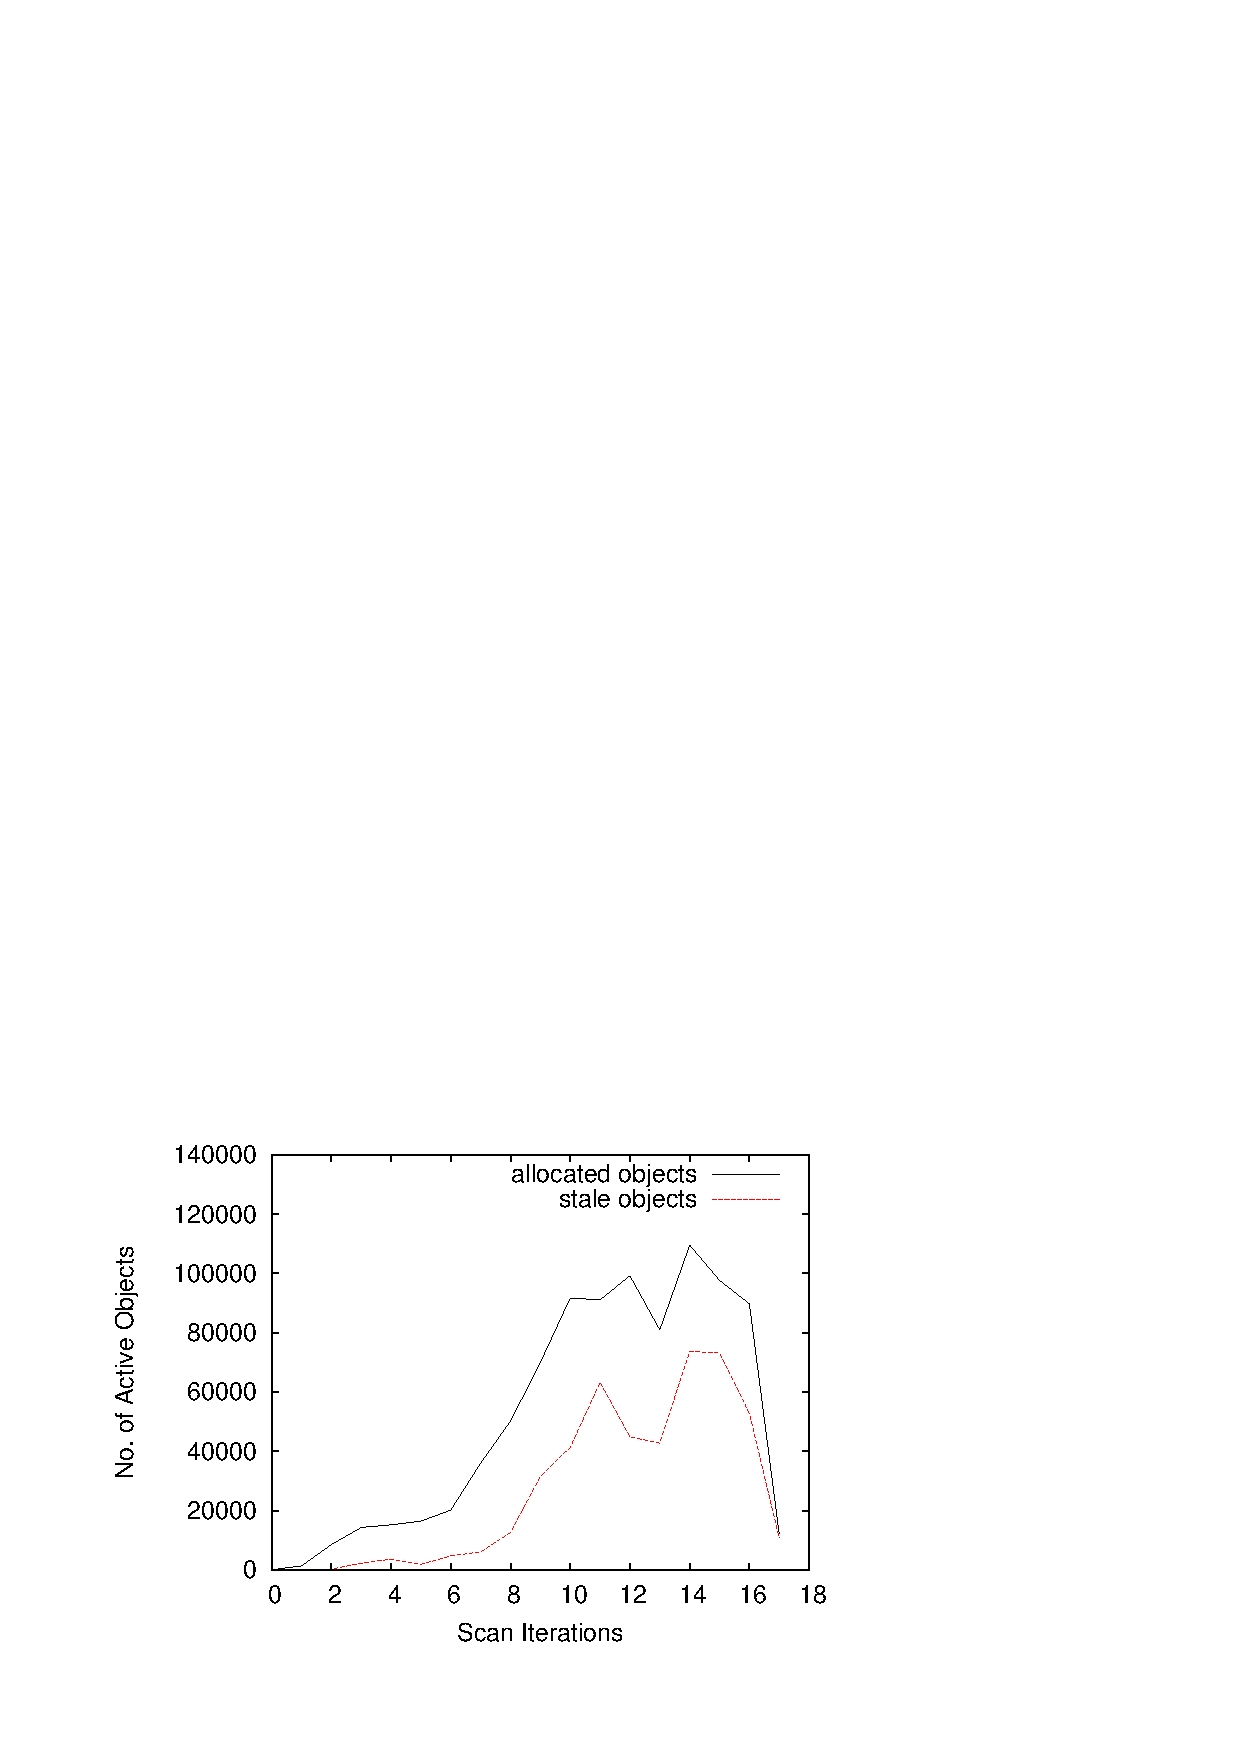
\includegraphics[width=6.0in]{stale_object.pdf}
\end{center}
%\vspace{-15pt}
\caption[Profile of stale object during leak scan.]{\label{fig:leak_detector-stale}The number of stale objects with increase in the number of allocated objects. The scanner thread was scheduled after every 100ms and the workload ran for 17 scan iterations.}
\end{figure}

\begin{table*}
\begin{center}
\begin{tabular}{|r|r|r|r|r|r|}
  \hline
  \multirow{2}{*}{scan} & \multirow{2}{*}{Allocated objects} & \multicolumn{2}{|c|}{Reachable objects} & \multicolumn{2}{|c|}{Unreachable objects} \\
  \hhline{~~----}
  & & Not Leaked & Leaked & Leaked & Not Leaked\\
  \hline
  1 & 27 & 19 & 0 & 8 & 0 \\
  \hline
  2 & 705 & 65 & 11 & 629 & 8 \\
  \hline
  3 & 1426 & 125 & 11 & 1290 & 18 \\
    \hline
  4 & 1824 & 221 & 10 & 1584 & 9 \\ \hline
  \hline
\end{tabular}
\caption[Profile of allocated objects with leak scan policies. The collector performs scan on all module reachable objects.]{\label{table:leak_detctor-leak_eval-policy2}The profile of the allocated objects and detected memory leaks when the scanner thread (collector) uses module reachable objects as ``root-set'' and performs reachability analysis.}
\end{center}
\end{table*}

\paragraph{Scanning of module reachable objects:} The policy considers all objects which are reachable from the module as ``root-set''. We used the same evaluation strategy for this policy and all memory deallocator functions from the \texttt{ext3} file system module are removed. Table~\ref{table:leak_detctor-leak_eval-policy2} shows that the policy detects actual leaks with less false positives and negatives.



\paragraph{Scanning of kernel heaps and static data:} This is the fall back policy for scanning and is not aggressive in nature.  Table~\ref{table:leak_detctor-leak_eval-policy3} shows that the policy reports a lot of false negative. However, it is fairly accurate in detecting leaks and an objects not found during this scan is definitely a leak.



\begin{table*}
\begin{center}
\begin{tabular}{|r|r|r|r|r|r|}
  \hline
  \multirow{2}{*}{scan} & \multirow{2}{*}{Allocated objects} & \multicolumn{2}{|c|}{Reachable objects} & \multicolumn{2}{|c|}{Unreachable objects} \\
  \hhline{~~----}
  & & Not Leaked & Leaked & Leaked & Not Leaked\\
  \hline
  1 & 59 & 52 & 28 & 7 & 0 \\
  \hline
  2 & 789 & 30 & 734 & 25 & 0 \\
  \hline
  3 & 805 & 30 & 305 & 470 & 0 \\
    \hline
  4 & 1623 & 24 & 797 & 802 & 0 \\ \hline
  \hline
\end{tabular}
\caption[Profile of allocated objects with leak scan policies. The collector performs scan on all kernel allocated pages.]{\label{table:leak_detctor-leak_eval-policy3}The profile of the allocated objects and detected memory leaks when the scanner thread (collector) scans all the kernel allocated pages.}
\end{center}
\end{table*}




\paragraph{compare with \emph{kmemleak}}
We also compared the performance of our leak detector with the overhead incurred by \emph{kmemleak}, a leak detector which operates on the whole kernel. We used server benchmarks from Filebench to evaluate performance. \Figref{leak_detector-kmemleak} shows that the performance of our leak detector is comparable to \emph{kmemleak} but our system has overhead only when the module is used where \emph{kmemleak} has overhead on the entire kernel. Also our leak scan policies are customizable and use fall back policy only when there is a constant increase in stale objects. \emph{kmemleak} always uses the fall back mechanism of scanning which is costly.


\begin{figure}[t]
\begin{center}
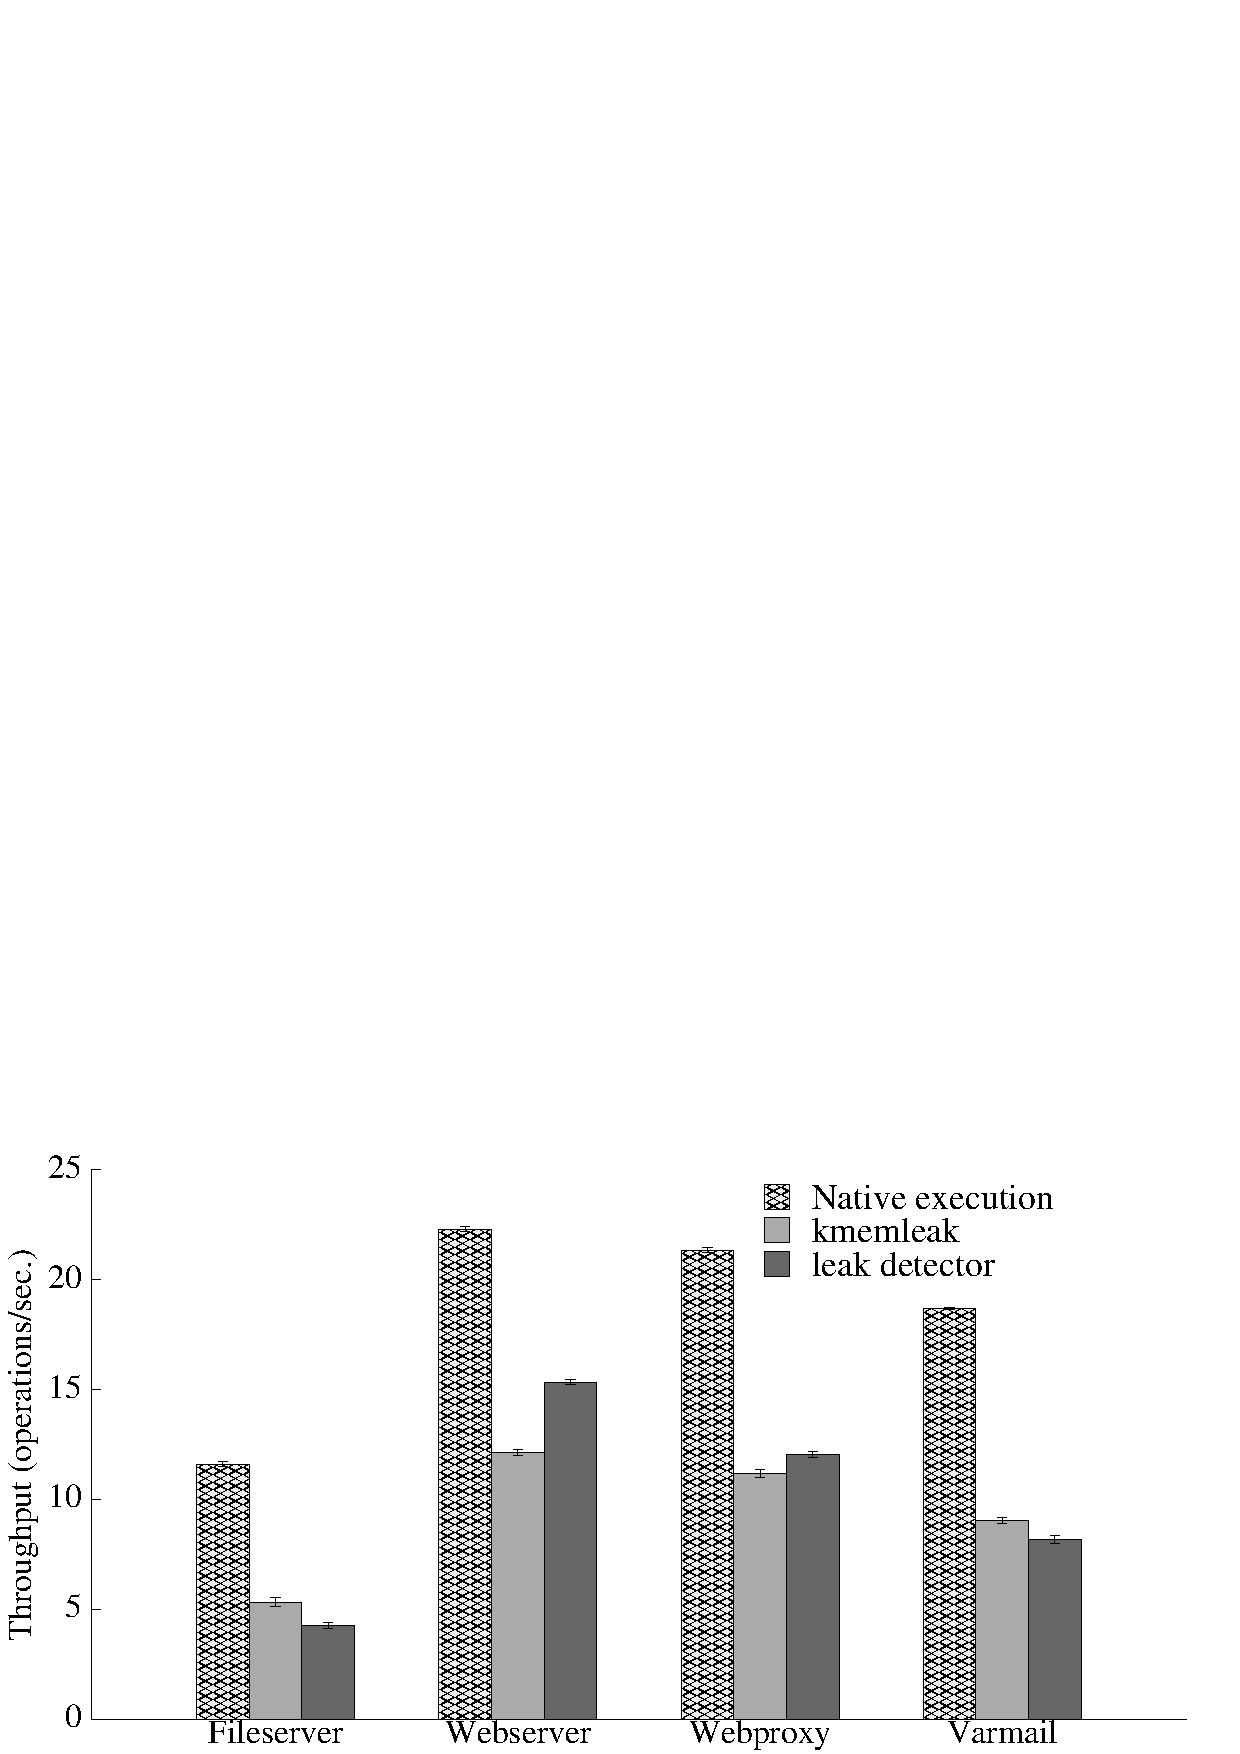
\includegraphics[width=6.0in,height=3.0in]{kmemleak.pdf}
\end{center}
\caption[Performance impact of leak detector on Filebench server benchmarks.]{\label{fig:leak_detector-kmemleak}The performance overhead of our leak detector when using the Filebench benchmark. It also compares the overhead of leak detector with \emph{kmemleak}, which operates on the entire kernel.}
\end{figure}


%\chapter{Results}\label{sec:results}
%\input{result}

\chapter{Related Work}\label{sec:related}
In this chapter, we discuss research topics that are related to our work. We first focus on the different solutions of implementing software and hardware watchpoints. We later look into the existing applications that can be used to detect memory errors.


\section{Watchpoints}
Watchpoints are an important debugging facility that help users identify data corruption bugs. There have been several proposals in the past on how to implement hardware and software watchpoints.


%We discuss several hardware and software watchpoints approaches below.
%This importance has been given due recognition and there has also been several proposals in the past on how to implement hardware and software watchpoints.
%in the form of hardware debug registers for watching memory locations implemented in almost all state-of-the-art processors. There has also been several proposals in the past on how to implement hardware and software watchpoints.

Greathouse \emph{et al.}~\cite{UnlimitedWatchpoints} propose a hardware solution that efficiently supports an unlimited number of watchpoints. Watchpoints are stored in main memory and utilize two different on-chip cache: a bitmap and a range cache, to accelerate performance. The bitmap lookaside buffer stores fine-grained watchpoints while the range cache can efficiently hold large contiguous regions of watchpoints and is useful for setting watchpoints on ranges of memory. 
%The design of low-overhead unlimited watchpoints helps support the varied needs of the wide range of dynamic analysis tools.
%It introduces two different on-chip caches: a bitmap and a range cache to handle spatial meradata pattern which gives it the benefits in terms of performance. 
Witchel and Asanovic~\cite{Mondrix} describe the implementation of the Mondriaan (also spelled Mondrian) memory protection domain system for the Linux kernel. Mondriaan was designed with fine-grained inter-process protection mechanism in mind, and is optimized for applications that do not perform frequent updates. The protection information is stored in main memory and is cached in a protection lookaside buffer (PLB). The implementation of protection domains using hardware enables fine- and coarse-grained memory protection, the mechanism which is similar to hardware watchpoints.

Zhou \emph{et al.}~\cite{Zhou:2004:IEA:998680.1006720} introduce intelligent Watcher (also known as iWatcher), which provides architectural support for monitoring program execution with minimum overhead. iWatcher stores per-word watchpoints alongside the cache lines that contain the watched data. These bits are initially set by hardware and are temporarily stored into a victim table on cache evictions. The hardware falls back to virtual memory watchpoints if this table overflows. iWatcher can watch a small number of ranges, which must be pinned in physical memory. If this range hardware overflows, the system falls back to setting a large number of per-word watchpoints. In general, this system is inadequate for tools that require more than a small number of large ranges.

Unlike behavioral watchpoints, these approaches depend on specialised hardware and require that applications using this hardware maintain context-specific information separately. 


Suh \emph{et al.} \cite{SecureProgramExecFlowTracking} propose a method of secure program execution by tracking dynamic information flow. Their method uses a one-bit tag to indicate whether the corresponding data block is \emph{authentic} or \emph{spurious}. The scheme can be extended to use multiple-bit tags if there are many types or sources of data.
Memory tagging at the hardware level allows their system to track tainted data as it propagates through a running program. Behavioral watchpoints are similar insofar as a watched address is tagged, and this tag propagates through a program.


%makes the case for supporting an unlimited number of watchpoints. A hardware solution is proposed and multiple applications are described. Unlike our approach, the cited approach depends on specialised hardware and requires that applications using these watchpoints maintain their own context-specific information.

%In , 

%\paragraph{Software-based}
Zhao \emph{et al.} \cite{DynamoRIOWatchpoints} describe a method for implementing an efficient and scalable DBT-based watchpoint system. It uses on-demand based dynamic instrumentation to accelerate the software debugger and supports more than a million watchpoints. It uses page protection and indirection through a hash table to track watched memory. This approach does not supports watching ranges of memory, or context-specific information. 


Lueck \emph{et al.} \cite{PinADX} introduce semantic watchpoints as part of the PinADX system, an extension of the PIN DBT framework. 
It enables interactive debugging by triggering debugger breakpoints when semantic conditions are met. While similar in spirit to behavioral watchpoints, semantic watchpoints do not maintain context-specific, per-watchpoint state. 

Wahbe \emph{et al.}~\cite{Wahbe:1992} also proposes the implementation of software watchpoint using code patching and static analysis. %Copperman and Thomas extended the work Wahbe and use a post-loading technique to insert checks into an executable to solve the shared library issue.
Another interesting approach, proposed by Keppel. \emph{et al.}~\cite{Keppel:93a} is to use checkpoints for memory updates. However all these approaches are valid for userspace programs only. The latest patches for MemCheck in Valgrind~\cite{Seward:2005} also introduce
support of adding watchpoint. They use data structure to maintain the watchlist and track the usage of watchpoints. This puts a severe restriction on their performance.   


\section{Memory Debugging}
There are many software, hardware or hybrid approaches proposed for detecting memory bugs. Purify~\cite{Rs_purify:fast} and MemCheck~\cite{Nethercote:2007:SBM:1254810.1254820} are two widely used software tools for detecting memory usage problems. Purify was one of the first tool to combine detection of memory leaks with detection of use-after-free errors. Purify uses a technique called object code insertion (OCI) to insert checking code around every instruction in an application that references, allocates, and deallocates memory. It uses a memory-coloring scheme to keep track of the state of every byte of memory in the application. The link time instrumentation and reporting reads of uninitialized errors immediately result in false positives. MemCheck~\cite{Nethercote:2007:SBM:1254810.1254820} is build on the Valgrind dynamic instrumentation framework. Dr. Memory is another memory checking tool developed using the DynamoRio instrumentation system. Both Memcheck and Dr Memory use a similar approach for tracking memory usage and both of them use Purify’s basic leak detection approach to detect memory leak errors.

The memory debugging tools developed using behavioral watchpoints also maintain the state of a memory block in its descriptor. The descriptor information gets encoded with the memory address and is directly available when the address is accessed.


Parallel Inspector~\cite{reference/parallel/Petersen11a} is a commercial tool built on the Pin~\cite{PinOS} dynamic instrumentation platform that combines data race detection with memory checking. But the details about its implementation are not publicly available. Insure++~\cite{Parasoft00INSU} is another commercial memory checking tool. It supports inserting instrumentation at various points, including in the source code prior to compile time, at link time, and at runtime, but its more advanced features require source code instrumentation. Insure++ also uses DBT-system to insert instrumentation at runtime. Unlike Insure++, Behavioral watchpoints does not require source code support for detecting memory errors. It uses a technique called reifying instrumentation to provide the benefits of high-level static analysis information in specialising instruction level instrumentation.

There have been several proposals to extend current hardware support for debugging memory related errors. DISE~\cite{Corliss:2005:LID:1042442.1043429} (Dynamic Instruction Steam Editing) is a general hardware mechanism for interactive debugging. It adds dynamic instructions for checking memory references into the instruction stream during execution. Other solutions such as SafeMem~\cite{Qin:2005:SEE:1042442.1043428}, iWatcher~\cite{Zhou:2004:IEA:998680.1006720}, and MemTracker~\cite{Venkataramani:2007:MEP:1317533.1318083} have also been proposed for detecting inappropriate usage of memory with low overhead. Unlike behavioral watchpoints, they require specialised hardware to implement their solutions. 

%For example, SafeMem exploits the use of ECC (Error-Correcting Code) for detecting memory leaks and memory corruption with low-overhead. But this approach relies on a write-allocate cache policy, i.e., the block is loaded on a write miss. One important drawback of these hardware approaches is that it requires customized, fixed-functionality hardware.





%Beside requiring customized hardware, it does not
%scale well as the number of checks increases when more
%watchpoints are set.


%HeapMon~\cite{Shetty:2006:HHA:1143264.1143273} is hardware/software approach for detecting memory bugs with the helper thread. Hardware such as SafeMem~\cite{Qin:2005:SEE:1042442.1043428}, iWatcher~\cite{Zhou:2004:IEA:998680.1006720}, and MemTracker~\cite{Venkataramani:2007:MEP:1317533.1318083} have also been proposed for detecting in appropriate usage of memory with low overhead. For example, SafeMem exploits the use of ECC (Error-Correcting Code) for detecting memory leaks and memory corruption with low-overhead. But this approach relies on a write-allocate cache policy, i.e., the block is loaded on a write miss. One important drawback of these hardware approaches is that it requires customized, fixed-functionality hardware.

%BoundsChecker~\cite{Jones97backwards-compatiblebounds} monitors Windows heap library calls and detects memory leaks and unaddressable accesses. It does
%not detect uninitialized reads. Some leak detection tools, including LeakTracer~\cite{Hauswirth:2004:LML:1024393.1024412} and mprof [6], only report memory that has not been freed at the
%end of execution. For these tools to be usable, the application
%must free all of its memory prior to exiting, even though it
%may have data whose lifetime is the process lifetime where it is
%more efficient to let the operating system free those resources.
%Reachability-based leak detection, in contrast, uses a memory
%scan that is similar to a mark-and-sweep garbage collector [3]
%to identify orphaned memory allocations that can no longer be
%accessed. This type of leak detection is used by most modern
%memory checking tools, including ours.

%There have been several hardware proposals to extend
%current hardware support for debugging. DISE~\cite{Corliss:2005:LID:1042442.1043429} (Dynamic
%Instruction Steam Editing) is a general hardware mechanism
%for interactive debugging. It adds dynamic instructions for
%checking memory references into the instruction stream during
%execution. Beside requiring customized hardware, it does not
%scale well as the number of checks increases when more
%watchpoints are set.



\chapter{Conclusion and Future Work}\label{sec:conclusions}
\input{conclusions}

%\chapter{Acknowledgements}
%We are indebted to Professors Ashvin Goel and Angela Demke Brown who
%guided us through this project. We are also extremely grateful to the
%rest of the DynamoRio-Kernel group for the extended discussion and
%assistance while debugging. We are also grateful to Dr Paul E. McKenney
%for his valuable input in deciding the goals of this project. Finally
%we are also extremely grateful to Professor Cristiana Amza for offering
%this course and allowing us to pursue this project.

%% This adds a line for the Bibliography in the Table of Contents.
\addcontentsline{toc}{chapter}{Bibliography}
%% *** Set the bibliography style. ***
%% (change according to your preference/requirements)
\bibliographystyle{plain}
%% *** Set the bibliography file. ***
%% ("thesis.bib" by default; change as needed)
\bibliography{thesis}

%% *** NOTE ***
%% If you don't use bibliography files, comment out the previous line
%% and use \begin{thebibliography}...\end{thebibliography}.  (In that
%% case, you should probably put the bibliography in a separate file and
%% `\include' or `\input' it here).

\end{document}
